% Template for PLoS
% Version 3.6 Aug 2022
%
% % % % % % % % % % % % % % % % % % % % % %
%
% -- IMPORTANT NOTE
%
% This template contains comments intended 
% to minimize problems and delays during our production 
% process. Please follow the template instructions
% whenever possible.
%
% % % % % % % % % % % % % % % % % % % % % % % 
%
% Once your paper is accepted for publication, 
% PLEASE REMOVE ALL TRACKED CHANGES in this file 
% and leave only the final text of your manuscript. 
% PLOS recommends the use of latexdiff to track changes during review, as this will help to maintain a clean tex file.
% Visit https://www.ctan.org/pkg/latexdiff?lang=en for info or contact us at latex@plos.org.
%
%
% There are no restrictions on package use within the LaTeX files except that no packages listed in the template may be deleted.
%
% Please do not include colors or graphics in the text.
%
% The manuscript LaTeX source should be contained within a single file (do not use \input, \externaldocument, or similar commands).
%
% % % % % % % % % % % % % % % % % % % % % % %
%
% -- FIGURES AND TABLES
%
% Please include tables/figure captions directly after the paragraph where they are first cited in the text.
%
% DO NOT INCLUDE GRAPHICS IN YOUR MANUSCRIPT
% - Figures should be uploaded separately from your manuscript file. 
% - Figures generated using LaTeX should be extracted and removed from the PDF before submission. 
% - Figures containing multiple panels/subfigures must be combined into one image file before submission.
% For figure citations, please use "Fig" instead of "Figure".
% See http://journals.plos.org/plosone/s/figures for PLOS figure guidelines.
%
% Tables should be cell-based and may not contain:
% - spacing/line breaks within cells to alter layout or alignment
% - do not nest tabular environments (no tabular environments within tabular environments)
% - no graphics or colored text (cell background color/shading OK)
% See http://journals.plos.org/plosone/s/tables for table guidelines.
%
% For tables that exceed the width of the text column, use the adjustwidth environment as illustrated in the example table in text below.
%
% % % % % % % % % % % % % % % % % % % % % % % %
%
% -- EQUATIONS, MATH SYMBOLS, SUBSCRIPTS, AND SUPERSCRIPTS
%
% IMPORTANT
% Below are a few tips to help format your equations and other special characters according to our specifications. For more tips to help reduce the possibility of formatting errors during conversion, please see our LaTeX guidelines at http://journals.plos.org/plosone/s/latex
%
% For inline equations, please be sure to include all portions of an equation in the math environment.  For example, x$^2$ is incorrect; this should be formatted as $x^2$ (or $\mathrm{x}^2$ if the romanized font is desired).
%
% Do not include text that is not math in the math environment. For example, CO2 should be written as CO\textsubscript{2} instead of CO$_2$.
%
% Please add line breaks to long display equations when possible in order to fit size of the column. 
%
% For inline equations, please do not include punctuation (commas, etc) within the math environment unless this is part of the equation.
%
% When adding superscript or subscripts outside of brackets/braces, please group using {}.  For example, change "[U(D,E,\gamma)]^2" to "{[U(D,E,\gamma)]}^2". 
%
% Do not use \cal for caligraphic font.  Instead, use \mathcal{}
%
% % % % % % % % % % % % % % % % % % % % % % % % 
%
% Please contact latex@plos.org with any questions.
%
% % % % % % % % % % % % % % % % % % % % % % % %

\documentclass[10pt,letterpaper]{article}
\usepackage[top=0.85in,left=2.75in,footskip=0.75in]{geometry}

% amsmath and amssymb packages, useful for mathematical formulas and symbols
\usepackage{amsmath,amssymb}

% Use adjustwidth environment to exceed column width (see example table in text)
\usepackage{changepage}

% textcomp package and marvosym package for additional characters
\usepackage{textcomp,marvosym}

% cite package, to clean up citations in the main text. Do not remove.
\usepackage{cite}

% Use nameref to cite supporting information files (see Supporting Information section for more info)
\usepackage{nameref,hyperref}

% line numbers
\usepackage[right]{lineno}
\usepackage{subcaption}

% ligatures disabled
\usepackage[nopatch=eqnum]{microtype}
\DisableLigatures[f]{encoding = *, family = * }

% color can be used to apply background shading to table cells only
\usepackage[table]{xcolor}

% array package and thick rules for tables
\usepackage{array}

% create "+" rule type for thick vertical lines
\newcolumntype{+}{!{\vrule width 2pt}}

% create \thickcline for thick horizontal lines of variable length
\newlength\savedwidth
\newcommand\thickcline[1]{%
  \noalign{\global\savedwidth\arrayrulewidth\global\arrayrulewidth 2pt}%
  \cline{#1}%
  \noalign{\vskip\arrayrulewidth}%
  \noalign{\global\arrayrulewidth\savedwidth}%
}

% \thickhline command for thick horizontal lines that span the table
\newcommand\thickhline{\noalign{\global\savedwidth\arrayrulewidth\global\arrayrulewidth 2pt}%
\hline
\noalign{\global\arrayrulewidth\savedwidth}}


% Remove comment for double spacing
%\usepackage{setspace} 
%\doublespacing

% Text layout
\raggedright
\setlength{\parindent}{0.5cm}
\textwidth 5.25in 
\textheight 8.75in

% Bold the 'Figure #' in the caption and separate it from the title/caption with a period
% Captions will be left justified
\usepackage[aboveskip=1pt,labelfont=bf,labelsep=period,justification=raggedright,singlelinecheck=off]{caption}
\renewcommand{\figurename}{Fig}

% Use the PLoS provided BiBTeX style
\bibliographystyle{plos2015}

% Remove brackets from numbering in List of References
\makeatletter
\renewcommand{\@biblabel}[1]{\quad#1.}
\makeatother



% Header and Footer with logo
\usepackage{lastpage,fancyhdr,graphicx}
\usepackage{epstopdf}
%\pagestyle{myheadings}
\pagestyle{fancy}
\fancyhf{}
%\setlength{\headheight}{27.023pt}
%\lhead{\includegraphics[width=2.0in]{PLOS-submission.eps}}
\rfoot{\thepage/\pageref{LastPage}}
\renewcommand{\headrulewidth}{0pt}
\renewcommand{\footrule}{\hrule height 2pt \vspace{2mm}}
\fancyheadoffset[L]{2.25in}
\fancyfootoffset[L]{2.25in}
\lfoot{\today}

%% Include all macros below

\newcommand{\lorem}{{\bf LOREM}}
\newcommand{\ipsum}{{\bf IPSUM}}

%% END MACROS SECTION


\begin{document}
\vspace*{0.2in}

% Title must be 250 characters or less.
\begin{flushleft}
{\Large
\textbf\newline{Title of submission to PLOS journals} % Please use "sentence case" for title and headings (capitalize only the first word in a title (or heading), the first word in a subtitle (or subheading), and any proper nouns).
}
\newline
% Insert author names, affiliations and corresponding author email (do not include titles, positions, or degrees).
\\
Name1 Surname\textsuperscript{1,2\Yinyang},
Name2 Surname\textsuperscript{2\Yinyang},
Name3 Surname\textsuperscript{2,3\textcurrency},
Name4 Surname\textsuperscript{2},
Name5 Surname\textsuperscript{2\ddag},
Name6 Surname\textsuperscript{2\ddag},
Name7 Surname\textsuperscript{1,2,3*},
with the Lorem Ipsum Consortium\textsuperscript{\textpilcrow}
\\
\bigskip
\textbf{1} Affiliation Dept/Program/Center, Institution Name, City, State, Country
\\
\textbf{2} Affiliation Dept/Program/Center, Institution Name, City, State, Country
\\
\textbf{3} Affiliation Dept/Program/Center, Institution Name, City, State, Country
\\
\bigskip

% Insert additional author notes using the symbols described below. Insert symbol callouts after author names as necessary.
% 
% Remove or comment out the author notes below if they aren't used.
%
% Primary Equal Contribution Note
\Yinyang These authors contributed equally to this work.

% Additional Equal Contribution Note
% Also use this double-dagger symbol for special authorship notes, such as senior authorship.
\ddag These authors also contributed equally to this work.

% Current address notes
\textcurrency Current Address: Dept/Program/Center, Institution Name, City, State, Country % change symbol to "\textcurrency a" if more than one current address note
% \textcurrency b Insert second current address 
% \textcurrency c Insert third current address

% Deceased author note
\dag Deceased

% Group/Consortium Author Note
\textpilcrow Membership list can be found in the Acknowledgments section.

% Use the asterisk to denote corresponding authorship and provide email address in note below.
* correspondingauthor@institute.edu

\end{flushleft}
% Please keep the abstract below 300 words
\section*{Abstract}
Lorem ipsum dolor sit amet, consectetur adipiscing elit. Curabitur eget porta erat. Morbi consectetur est vel gravida pretium. Suspendisse ut dui eu ante cursus gravida non sed sem. Nullam sapien tellus, commodo id velit id, eleifend volutpat quam. Phasellus mauris velit, dapibus finibus elementum vel, pulvinar non tellus. Nunc pellentesque pretium diam, quis maximus dolor faucibus id. Nunc convallis sodales ante, ut ullamcorper est egestas vitae. Nam sit amet enim ultrices, ultrices elit pulvinar, volutpat risus.


% Please keep the Author Summary between 150 and 200 words
% Use first person. PLOS ONE authors please skip this step. 
% Author Summary not valid for PLOS ONE submissions.   
\section*{Author summary}
Lorem ipsum dolor sit amet, consectetur adipiscing elit. Curabitur eget porta erat. Morbi consectetur est vel gravida pretium. Suspendisse ut dui eu ante cursus gravida non sed sem. Nullam sapien tellus, commodo id velit id, eleifend volutpat quam. Phasellus mauris velit, dapibus finibus elementum vel, pulvinar non tellus. Nunc pellentesque pretium diam, quis maximus dolor faucibus id. Nunc convallis sodales ante, ut ullamcorper est egestas vitae. Nam sit amet enim ultrices, ultrices elit pulvinar, volutpat risus.

\linenumbers

\section*{Introduction}\label{sec1}
Traditionally, for down stream tasks related to protein structure (e.g., protein structure classification), features were directly extracted from the 3d structure of proteins. For instance, Cui and Lui~\cite{ciu20083dprotein} consider the geometrical properties of a protein structure by viewing a protein molecule to be comprising of several cube-like regions and computing probability based statistics of atoms belonging to different regions. However, this kind of feature representation does not capture connectivity properties of atoms/ amino acids. Representing protein structure as graph of atoms/ amino acid residues where edges capture connectivity between amino acids can provide insights into protein folding as network based approaches can be applied to this graph. 

\section*{Single layer networks}
Protein structure networks are graphs in which nodes represent amino acid residues and edges capture relationships--based on factors such as interaction energy and proximity--between the amino acids~\cite{vijayabaskar2010interaction, bhattacharyya2016function}. As opposed to directly extracting geometrical properties of a protein structure using the protein's structural coordinates, a graph-based representation has been found to be beneficial in its mathematical formalism to perform network analysis~\cite{schieber2017network}. Furthermore, much work has been performed using graph based spectral methods to compare performance of such methods with traditional methods that use structural topologies~\cite{bhattacharyya2013automated, chakrabarty2014repeat, gadiyaram2017spectral}. 

\subsection*{Graph spectral method for comparing protein structures}
Generally, networks can be exactly matched using techniques such as subgraph isomorphism (i.e., given two graphs, determine whether one graph contains a subgraph of the other and is isomorphic or that there is a one-to-one mapping of the vertices between the two graphs such that edge connections are preserved), clique detection~\cite{gadiyaram2017spectral}. For inexact matching of networks, graph edit distance can be used. Spectral methods that compare networks by approximately matching the clusters capturing local structural properties include k-means based on Fiedler vectors (note that a Fiedler vector of a graph is the  eigenvector corresponding to the second smallest eigenvalue) and main components in principle component analysis~\cite{gadiyaram2017spectral}. Gadiyaram et al.~\cite{gadiyaram2017spectral} develop a network comparison score that captures differences at both the local edge level as well as at the global cluster level, unlike eigenvalue based methods that cannot differentiate between isomorphic networks and Hamming distance based methods that do not capture differences in clustering of networks (e.g.,~\cite{jurman2015him, jurman2011spectral}). 

\subsubsection*{Network similarity score~\cite{gadiyaram2017spectral}}
Graphs can be represented as matrices taking on various forms such as adjacency, Laplacian, and normalized Laplacian~\cite{butler2006spectral, butler2015laplacian, chung1997spectral, luxburg2007spectral, zumstein2005spectral}. In spectral graph theory, graphs are represented as matrices and algebraic tools are applied to these matrices to capture various structural aspects of the graphs. Let $G=(V,E)$ be a graph with $|V|=n$ (where $n$ is the number of vertices in the $G$), $A_G$ be $n \times n$ matrix where $A_G(i,j)=1$ iff $(i,j) \in G$, and $D_G$ be the degree matrix where $D_G(i,i)$ is the degree of vertex $i$ in $G$ and is a diagonal matrix. Then, the Laplacian $L$ of graph $G$ is defined as $L_G$ = $D_G$-$A_G$. 

% \subsection{Network parameters}
% Diameter, centrality, shortest path length, clustering coefficient, subgraph identification, coefficient of assortativity, walk characteristics, Markov clustering

\section*{Multilayer networks}

% \subsection{Different kinds of problems and taxonomy}
% 1. subgraph identification 2. hiding such that centrality is not necessarily high *3. centrality measure and multicentrality 4. infer causal relations between nodes 5. handling time varying interconnections (dynamic multilayer networks) 6. borrowing information within each network (capturing dependence) across time between layers 7. link/ edge prediction (cross-network embedding, gnn, node-pair structural features, node embedding similarity) *8. supervised community detection 9. (topological) clustering 10. unsupervised learning of multilayer networks *11. percolation (combinatorics) and resilience of multilayer networks *12. diffusion in multilayer networks *13. interdependent networks *14. robustness of multilayer networks during failure *15. epidemic spreading mechanism and information diffusion 16. concept and terminologies: network, graph, vertex node, layer, intra-layer edge, inter-layer edge, interlayer, multilayer 17. interactions: endogenous distinct vertices within same layer, exogenous distinct vertices in distinct layers represent distinct nodes, intertwining distinct vertices in distinct layers representing same node 18. taxonomy of multilayer graphs: edge colored graphs self and endogenous, multiplex graphs self, endogenous, and intertwining, interdependent self, endogenous, and exogenous, general interconnected *19. community detection 20. coverage evolution 21. multiplex networks with different nodes and different edge types can be disentangled to multilayer networks 22. network of networks: interactions between one node to many nodes or one node *23. tensor representation: finding principal components 24. network alignment 25. node similarity 26. multimodal networks 27. hierarchy-aware unsupervised node feature learning 28. applications of multilayer networks in bioinformatics 29. ranking 30. nature, bioinformatics, aaai, ijcai, nips, icml, www, ismb, briefings in bioinformatics, nucleic acid research, BIBM, BCB 31. protein complexes, protein structure networks - identify community and dense subgraphs 32. heterogeneous network structure learning (heterogeneous, inter intra, features) 33. Real-time structure search and structure classification for AlphaFold protein models 34. Multiplex Graph Association Rules for Link Prediction

\subsection*{Heterogeneous graphs for biological complex scoring}
Understanding interactions between molecules of proteins is one of the main aspects in identifying proteins as drug targets~\cite{xie2023undruggable}. Crampon et al.~\cite{crampon2023heterogeneous} propose a new scoring function to capture the affinity between a protein and a ligand (i.e, any chemical compound). One of the applications is molecular docking where the affinity score is used to predict the likelihood of a ligand (i.e., a small molecule) will bind to a protein (i.e., a macro molecule or a receptor). This method can be applied to other biological complexes such as protein-protein, protein-sugar, protein-dna, etc. Typically, to predict the affinity score of the complex, either the protein-protein interaction network or the structure of the molecules is used. 

\subsection*{Protein structure classification}
One of the ways to classify protein structures is by using network level features (e.g., graphlet features) extracted using the protein structure network~\cite{khalique2022multilayer}. Since structure of a protein hugely influences the protein's functions, the structure classification can be used to further predict protein function. Another approach for structure classification is by using protein sequence features~\cite{jiaqi2016ensemble}. However, it has has been discussed that proteins with low sequence similarity can have similar 3-d structures~\cite{sousounis2012conservation, kosloff2008sequence}. Thus, protein sequence and structure data can be used complementary to each other for the task of protein structure classification. 

Newaz et al.~\cite{khalique2022multilayer} propose a multilayer sequential network model to classify protein structures. Give a protein domain (i.e., a sequence of amino acids), they construct multiple unweighted graphs (in which nodes are amino acids and edges denote distances between amino acids) using incremental subsequences of the protein domain. Each graph capturing a snapshot of the domain represents a layer in the multilayer network. For protein structure classification, features extracted from the multilayer network include dynamic graphlet degree~\cite{hulovatyy2015structure} and graphlet orbit transition~\cite{aparicio2018transitions, aparicio2019network}. 


\subsection*{Why multilayer networks to model protein complexes}
Say we have two sets of disjoint nodes, $m$ and $n$, in a single-layer graph, the total number of possible edges between all nodes is $m+n \choose 2$. There are no constraints on how these edges are distributed, as in any node can connect to any other node. In a multilayer graph, the graph is split into 2 distinct layers, each with its own set of nodes $m$ and $n$. The edges are divided into: connections within each layer or intralayer edges and connections between nodes in different layers. Intralayer edges are constrained to a maximum of $m \choose 2$ edges in the first layer and $n \choose 2$ edges in the second layer. Maximum number of interlayer edges is $m \times n$, as each node in the first layer can connect to every node in the second layer. 

However, presence or absence of interlayer edges often depends on relationships within the individual layers. Nodes in one layer may only connect to nodes in the other layer if there is a certain property (e.g., closeness, similarity, or shared features) established by their intralayer edges. This introduces dependencies between interlayer and intralayer edge configurations, imposing constraints. 

In a single-layer graph, all $m+n \choose 2$ edges are independent, and no specific relationships govern their presence. In a multilayer graph, the structure of the layers directly influences the presence and pattern of interlayers edges. The total edge distribution is shaped by both layer-specific constraints and cross-layer relationships. The resulting graph has far fewer possible configurations than a single-layer graph with the same number of nodes. 

Intuitively, in a single layer setting, all individual residues in a protein complex can connect to any residues without restrictions. In a multilayer setting, connections between  residues across two chains exist only if they are already part of some underlying structures in their individual chains. That is, in a multilayer setting, a significantly more number of interlayer configurations (out of the possible $m \times n$) are ruled out versus in a single layer setting. For instance, in Clock-Bmal2 complex, there are 354 residues in Clock and 374 residues in Bmal2. While there are $\sim$2.5k edges in individual proteins, there are only $\sim$100 edges across them. 

Interlayer edges often reflect binding characteristics of residues across chains based on properties within the individual chains such as density or connectively of intra-chain edges, structural similarity of intralayer properties of residues (e.g. Jaccard similarity, residues are similar if their neighborhoods in their respective chains are similar), interchain edges exist only if residues meet some kind of a threshold crieria derived from intrachain connectively, interchain edges are formed preferentially between residues that belong to similar or overlapping communities within their chains (e.g., Louvain or Infomap to identify residue communities within each layer; interchain edge presence depends on the overlap of node community memberships), or interchain edges reflect the flow of influence or information across layers, based on some underlying intrachain dynamics. 

\begin{figure}[h!]
	\centering
	\begin{minipage}[b]{0.25\linewidth}
		\centering
		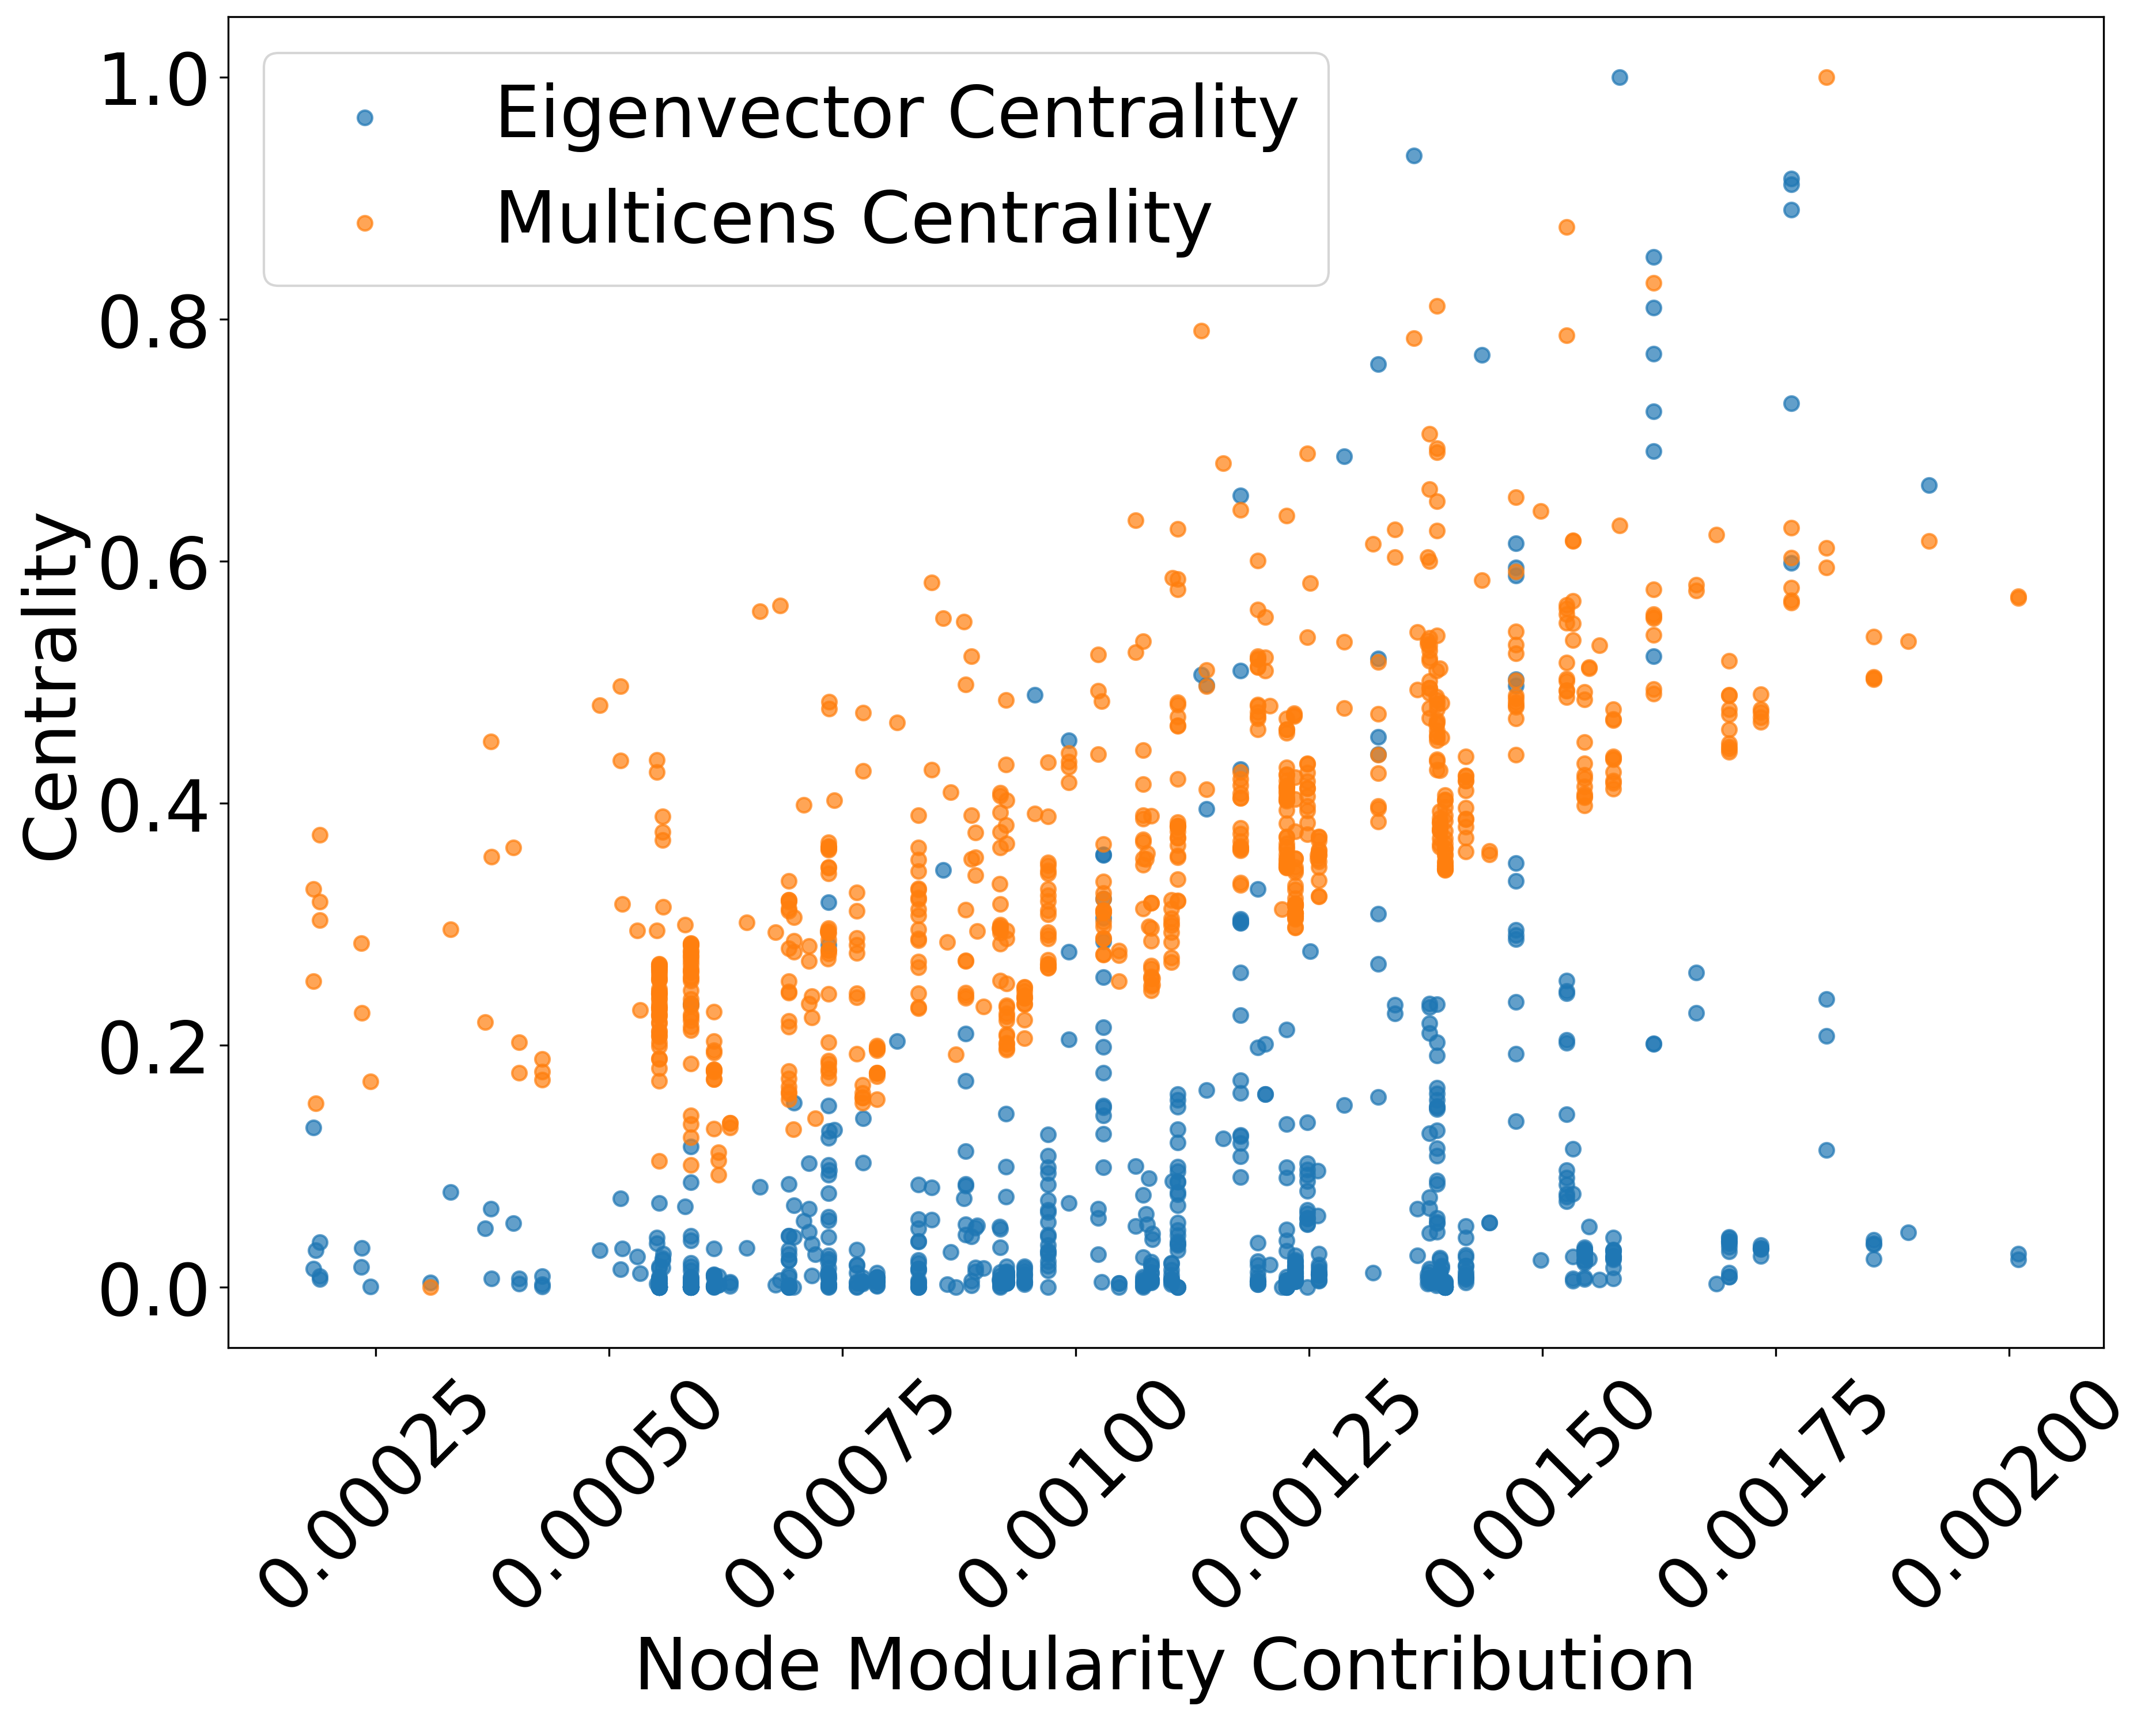
\includegraphics[width=\textwidth]{figs/fig1.png}
		\subcaption{}
	\end{minipage}
	\hspace{0.5cm}
	\begin{minipage}[b]{0.25\linewidth}
		\centering
		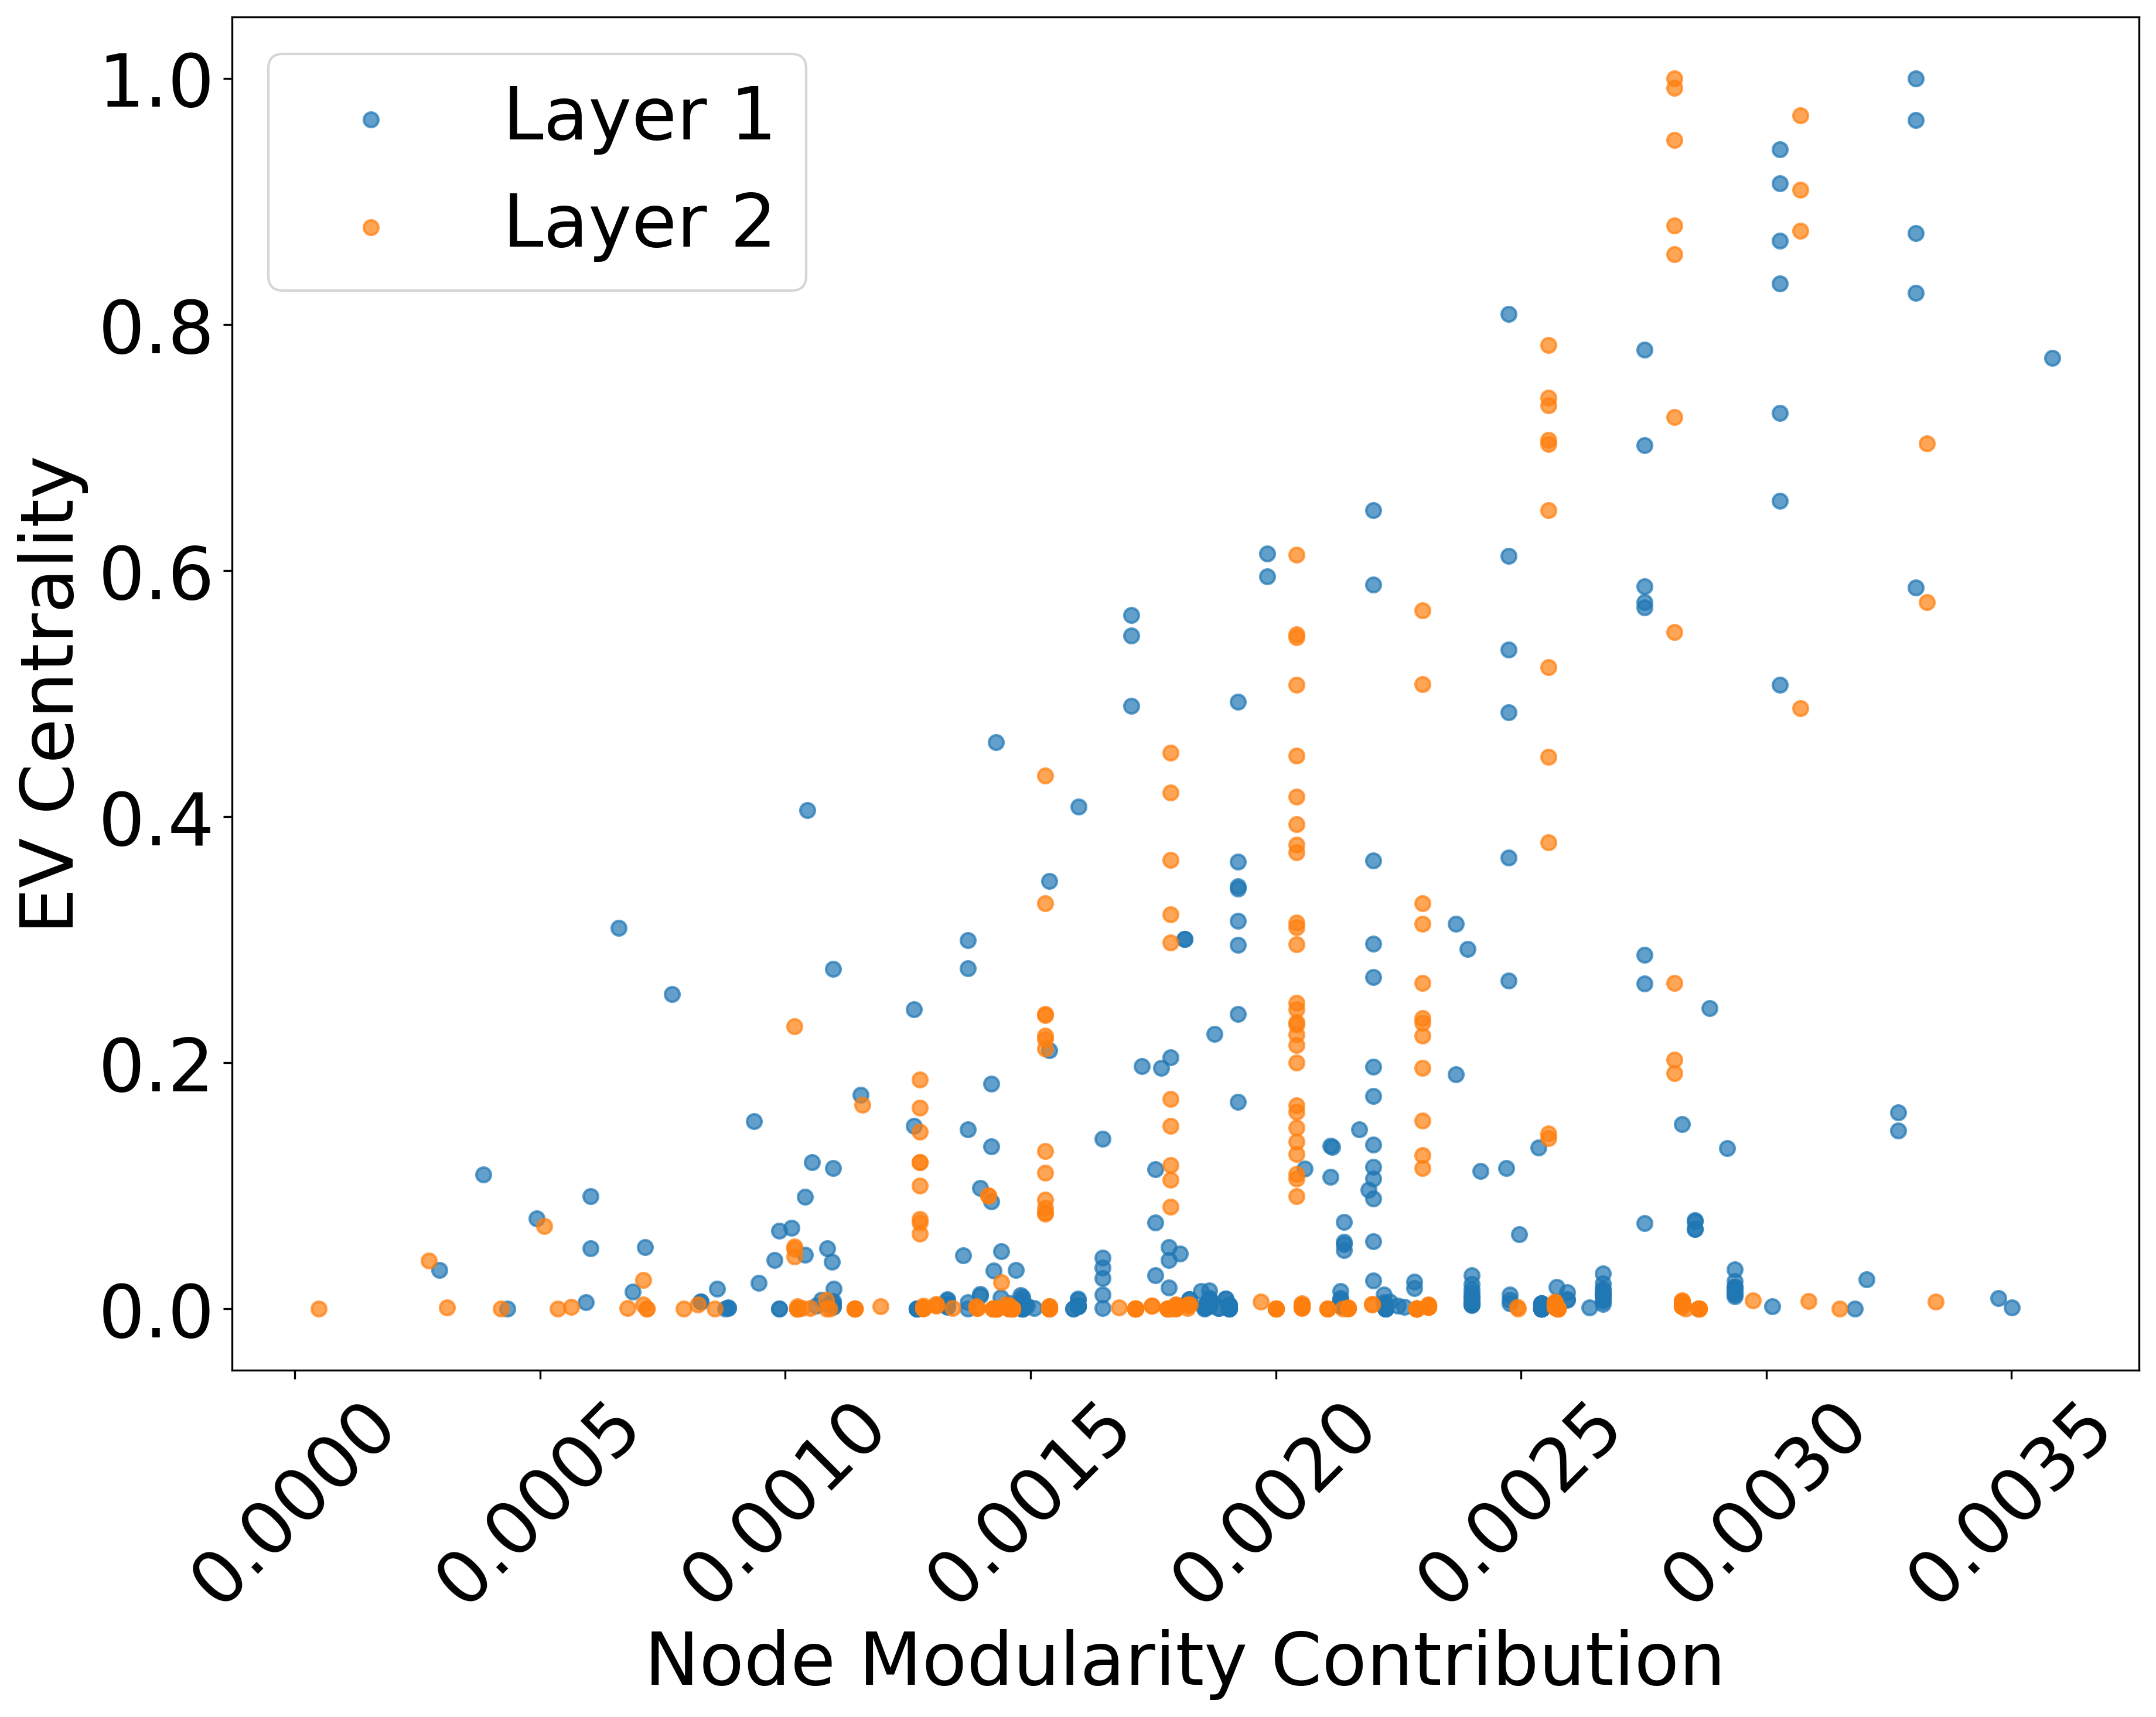
\includegraphics[width=\textwidth]{figs/fig2.png}
		\subcaption{}
	\end{minipage}
	\hspace{0.5cm}
	\begin{minipage}[b]{0.25\linewidth}
		\centering
		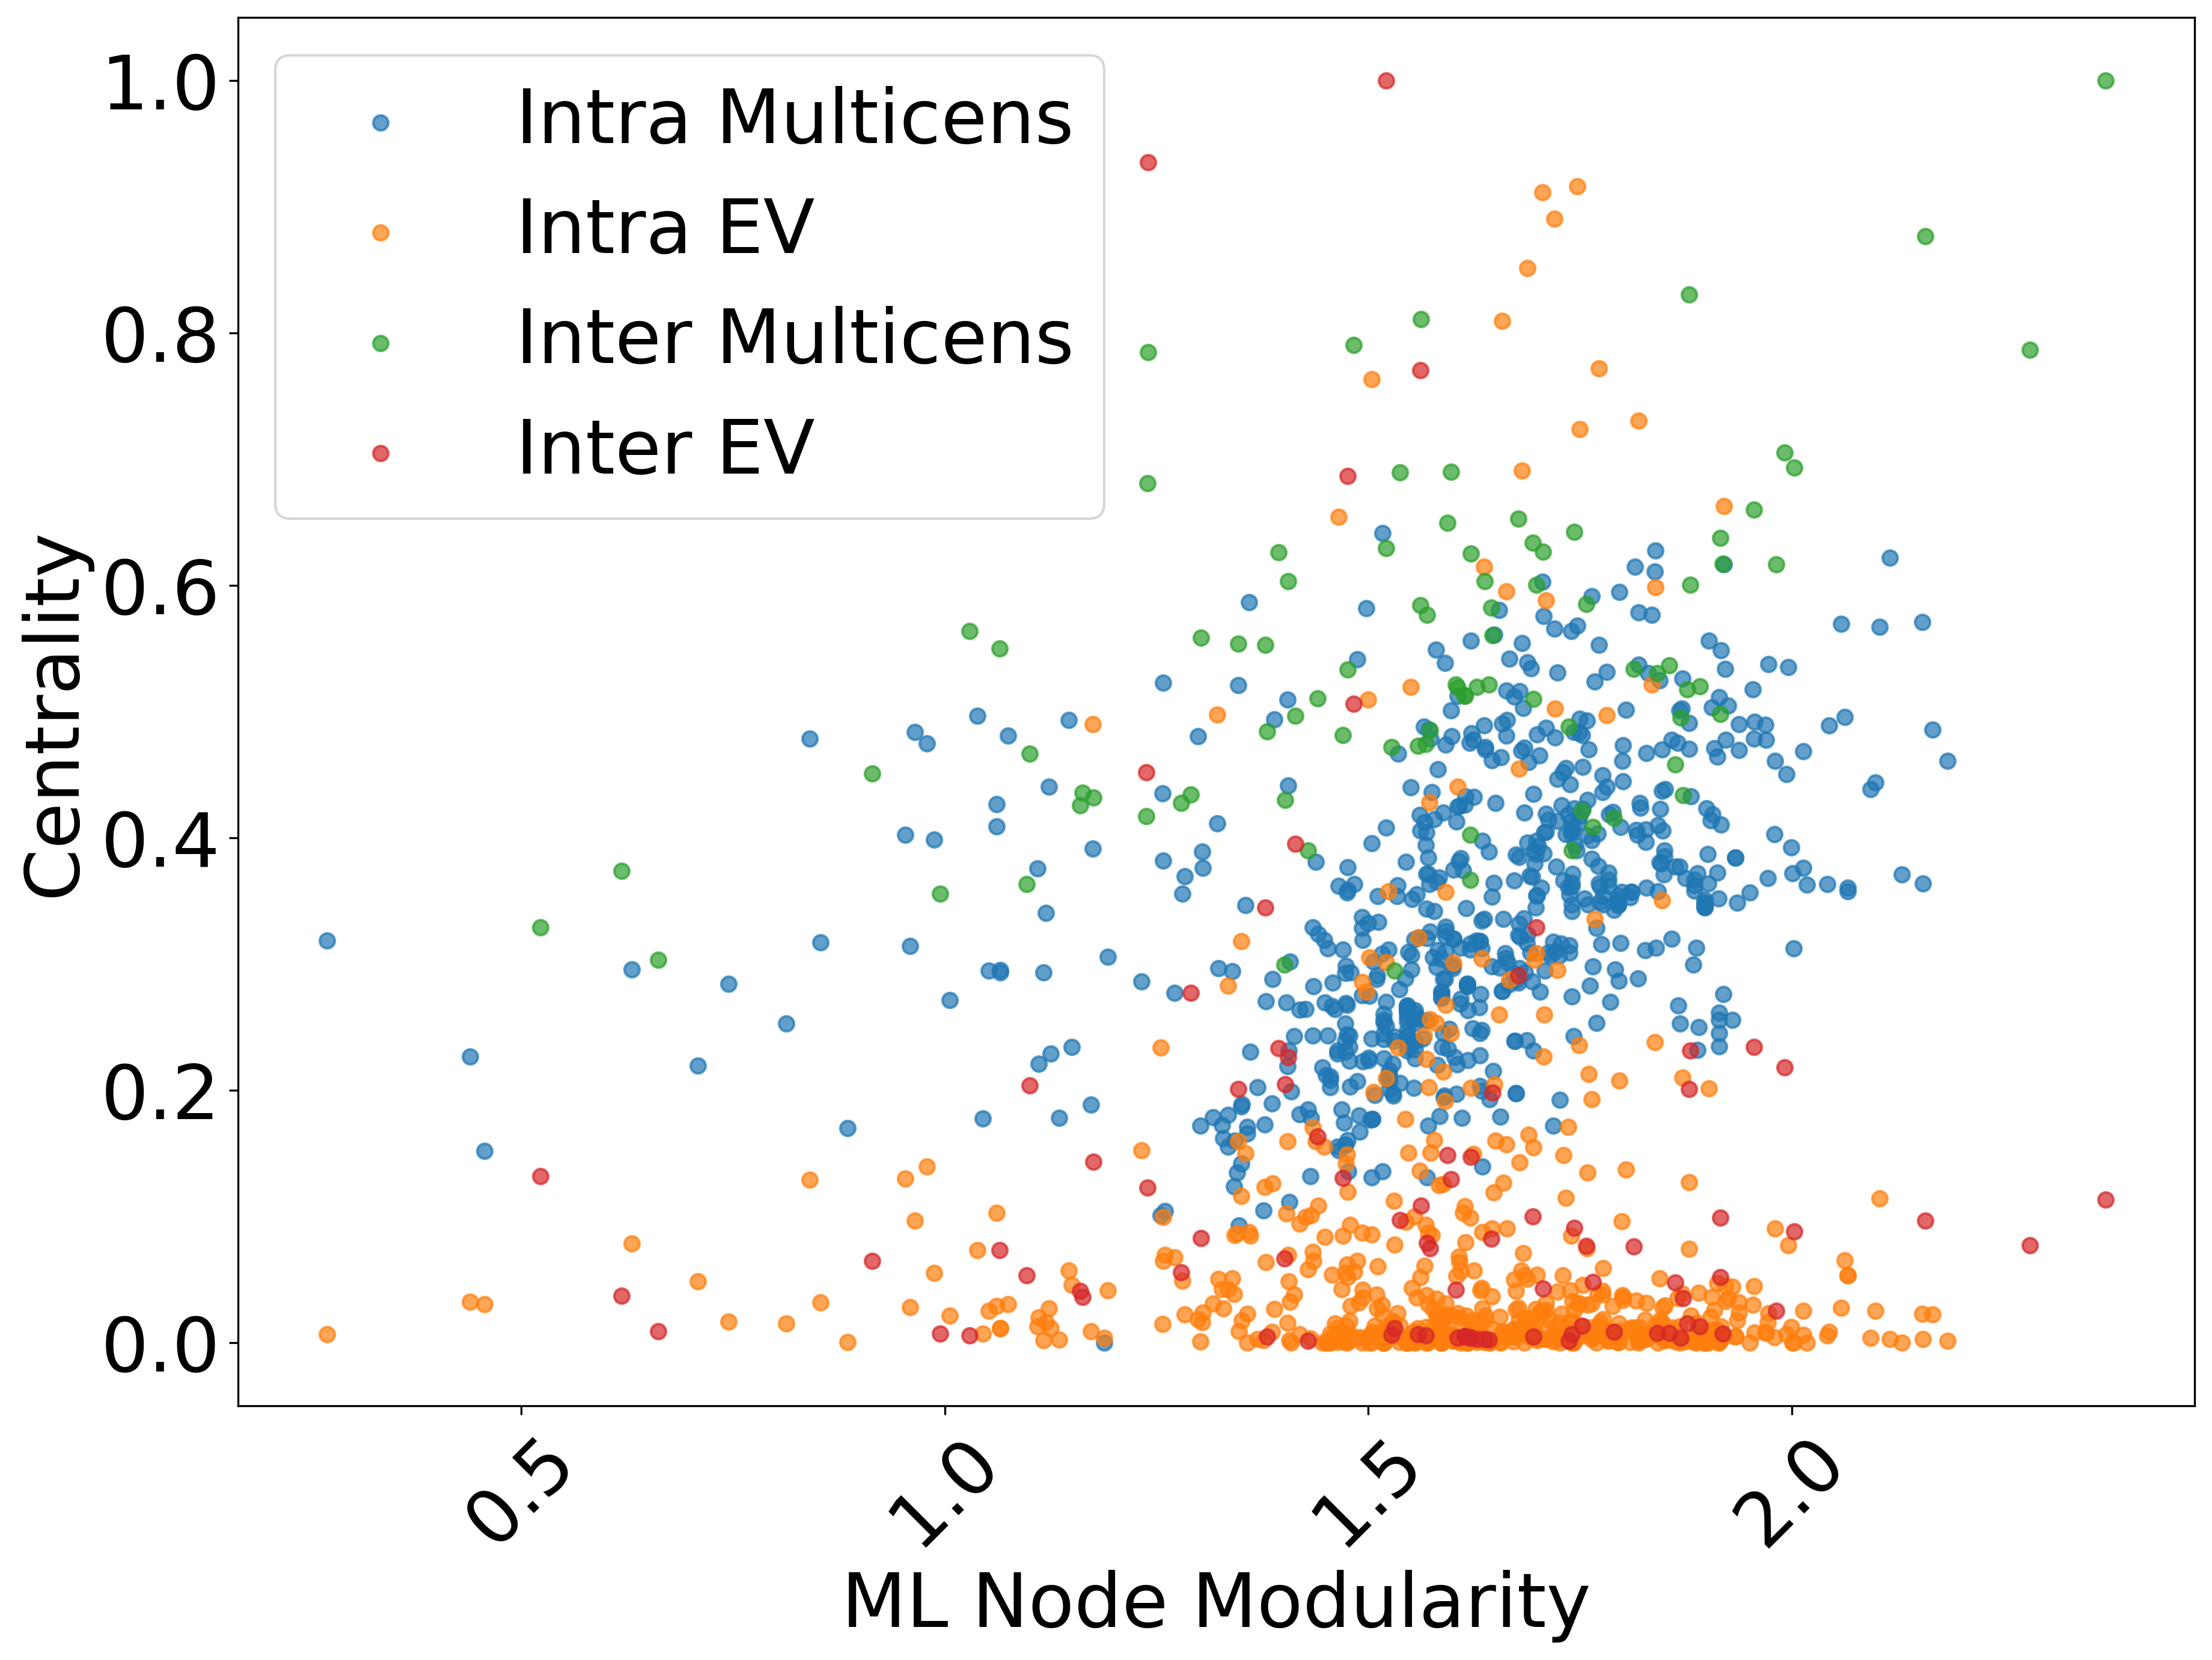
\includegraphics[width=\textwidth]{figs/fig3.png}
		\subcaption{}
	\end{minipage}
	
	\vspace{0.5cm}
	
	\begin{minipage}[b]{0.25\linewidth}
		\centering
		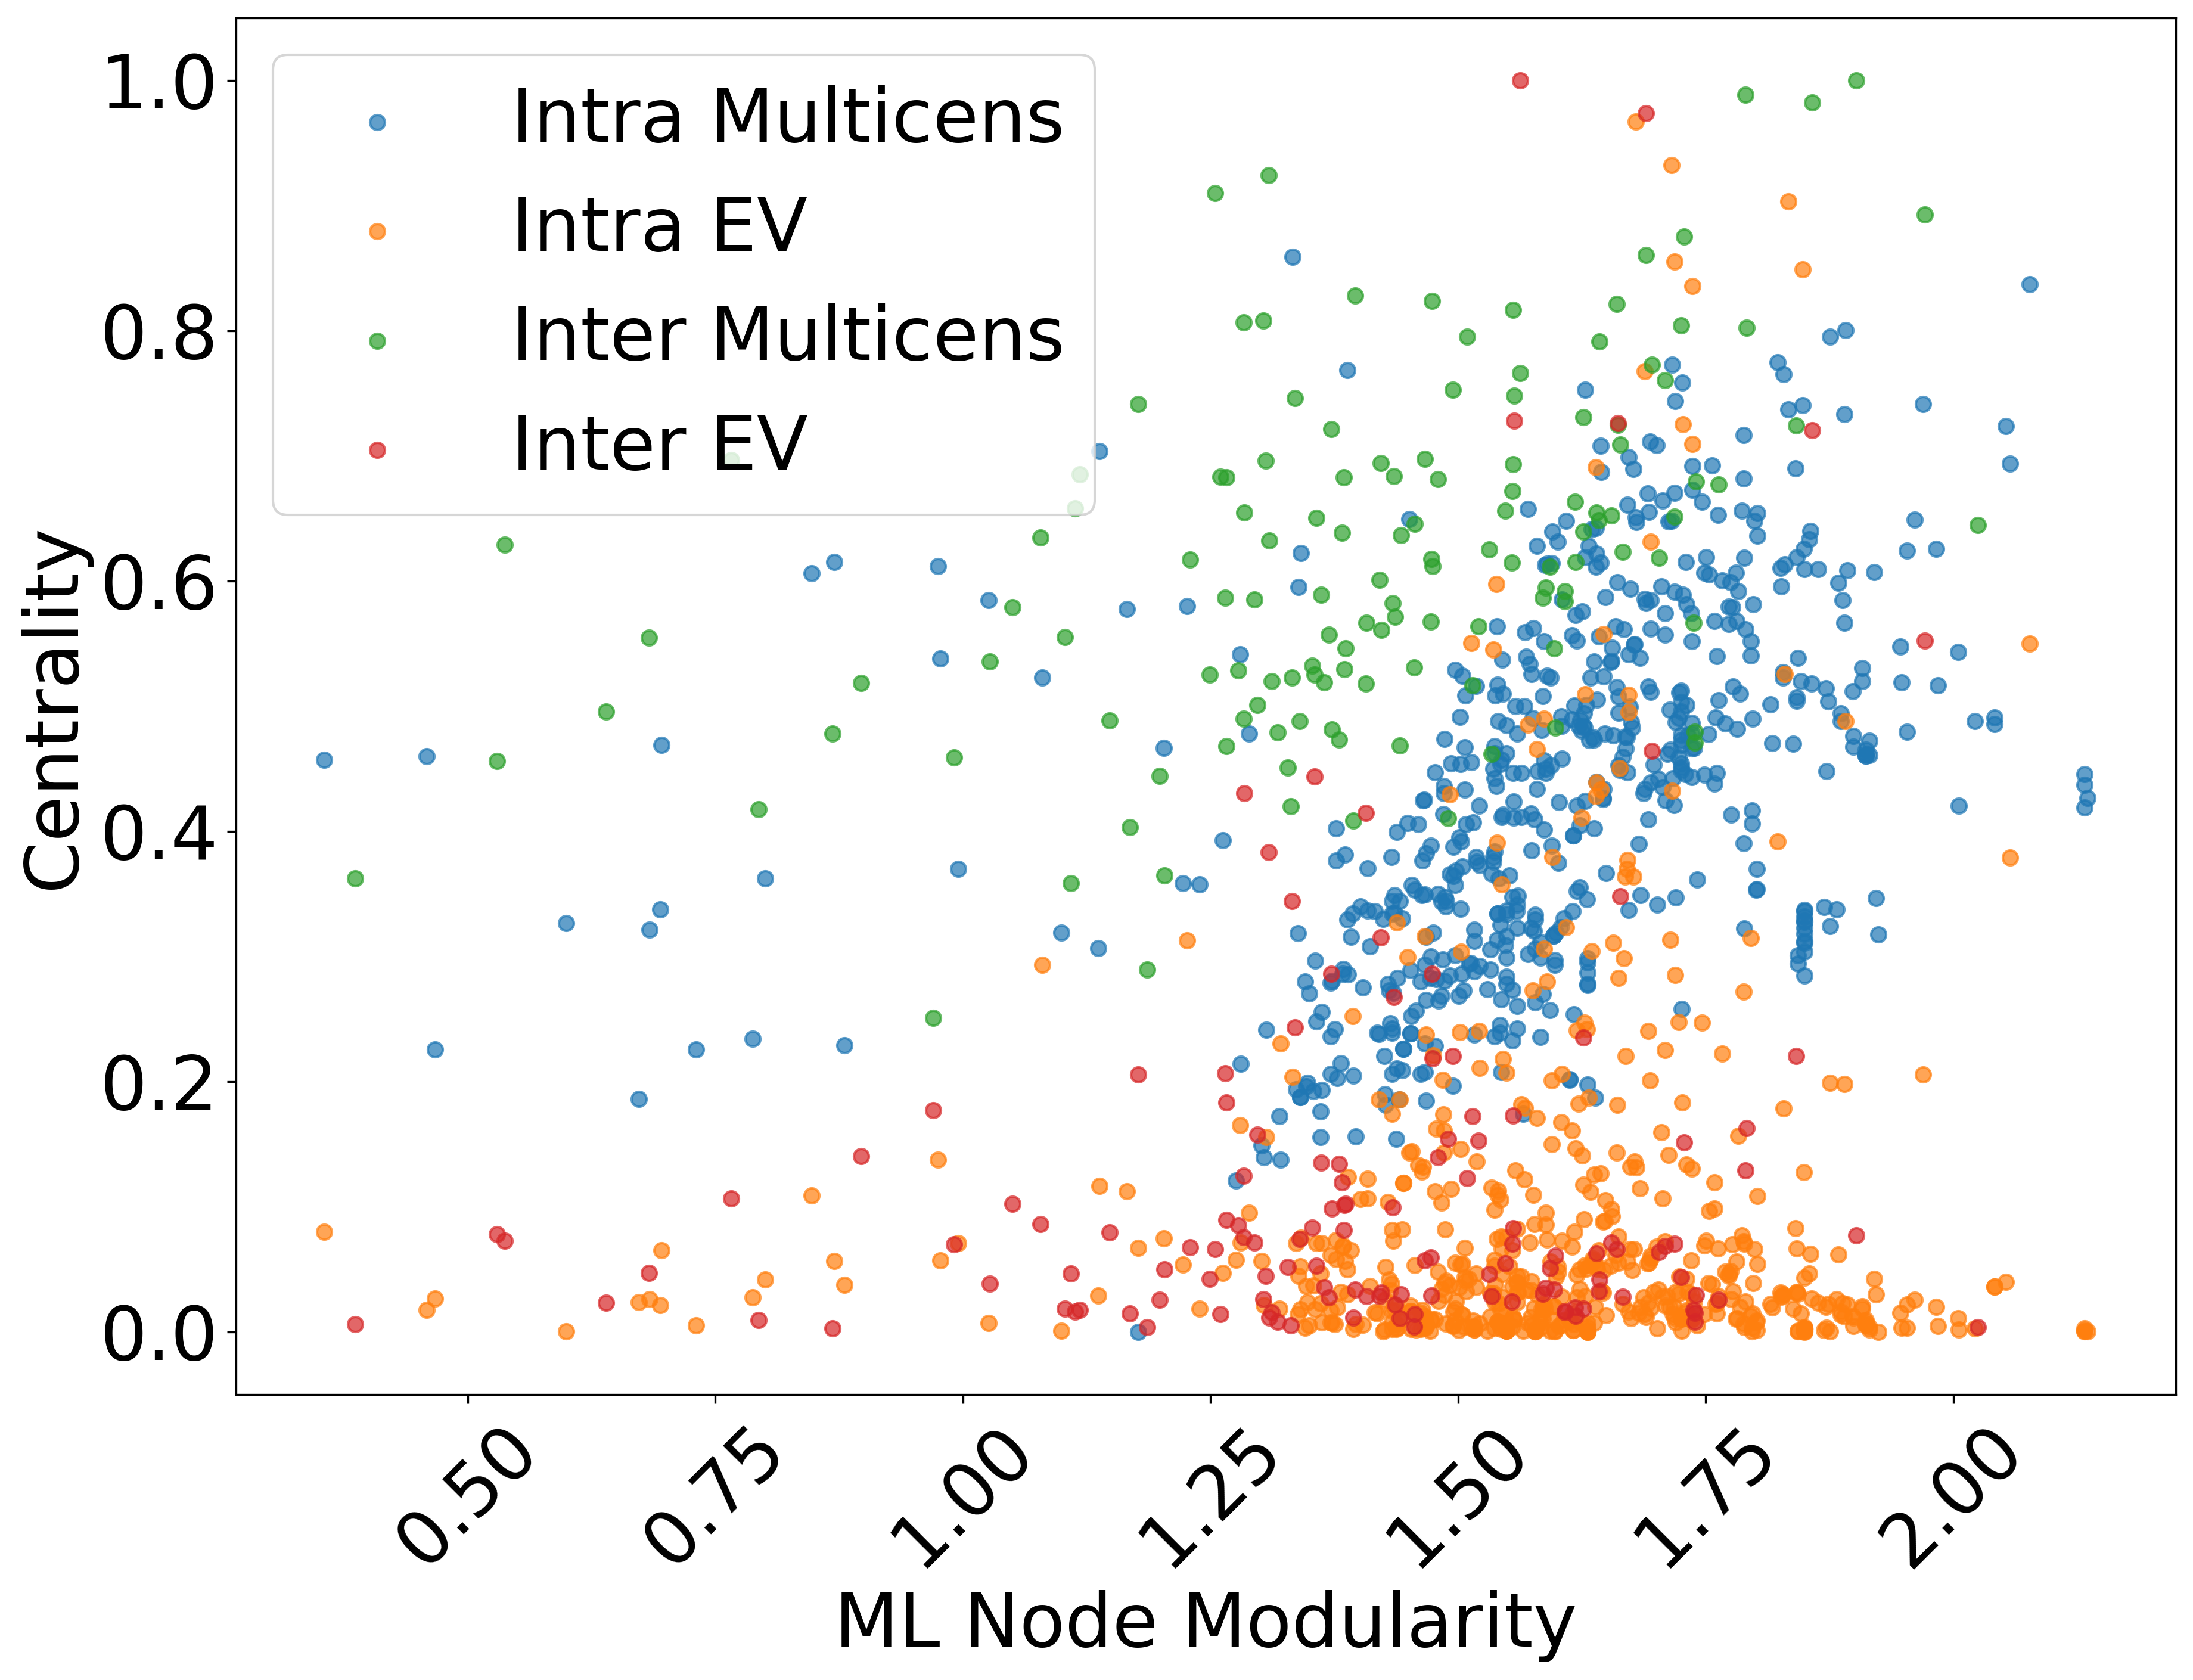
\includegraphics[width=\textwidth]{figs/fig4.png}
		\subcaption{}
		\label{fig4}
	\end{minipage}
	\hspace{0.5cm}
	\begin{minipage}[b]{0.25\linewidth}
		\centering
		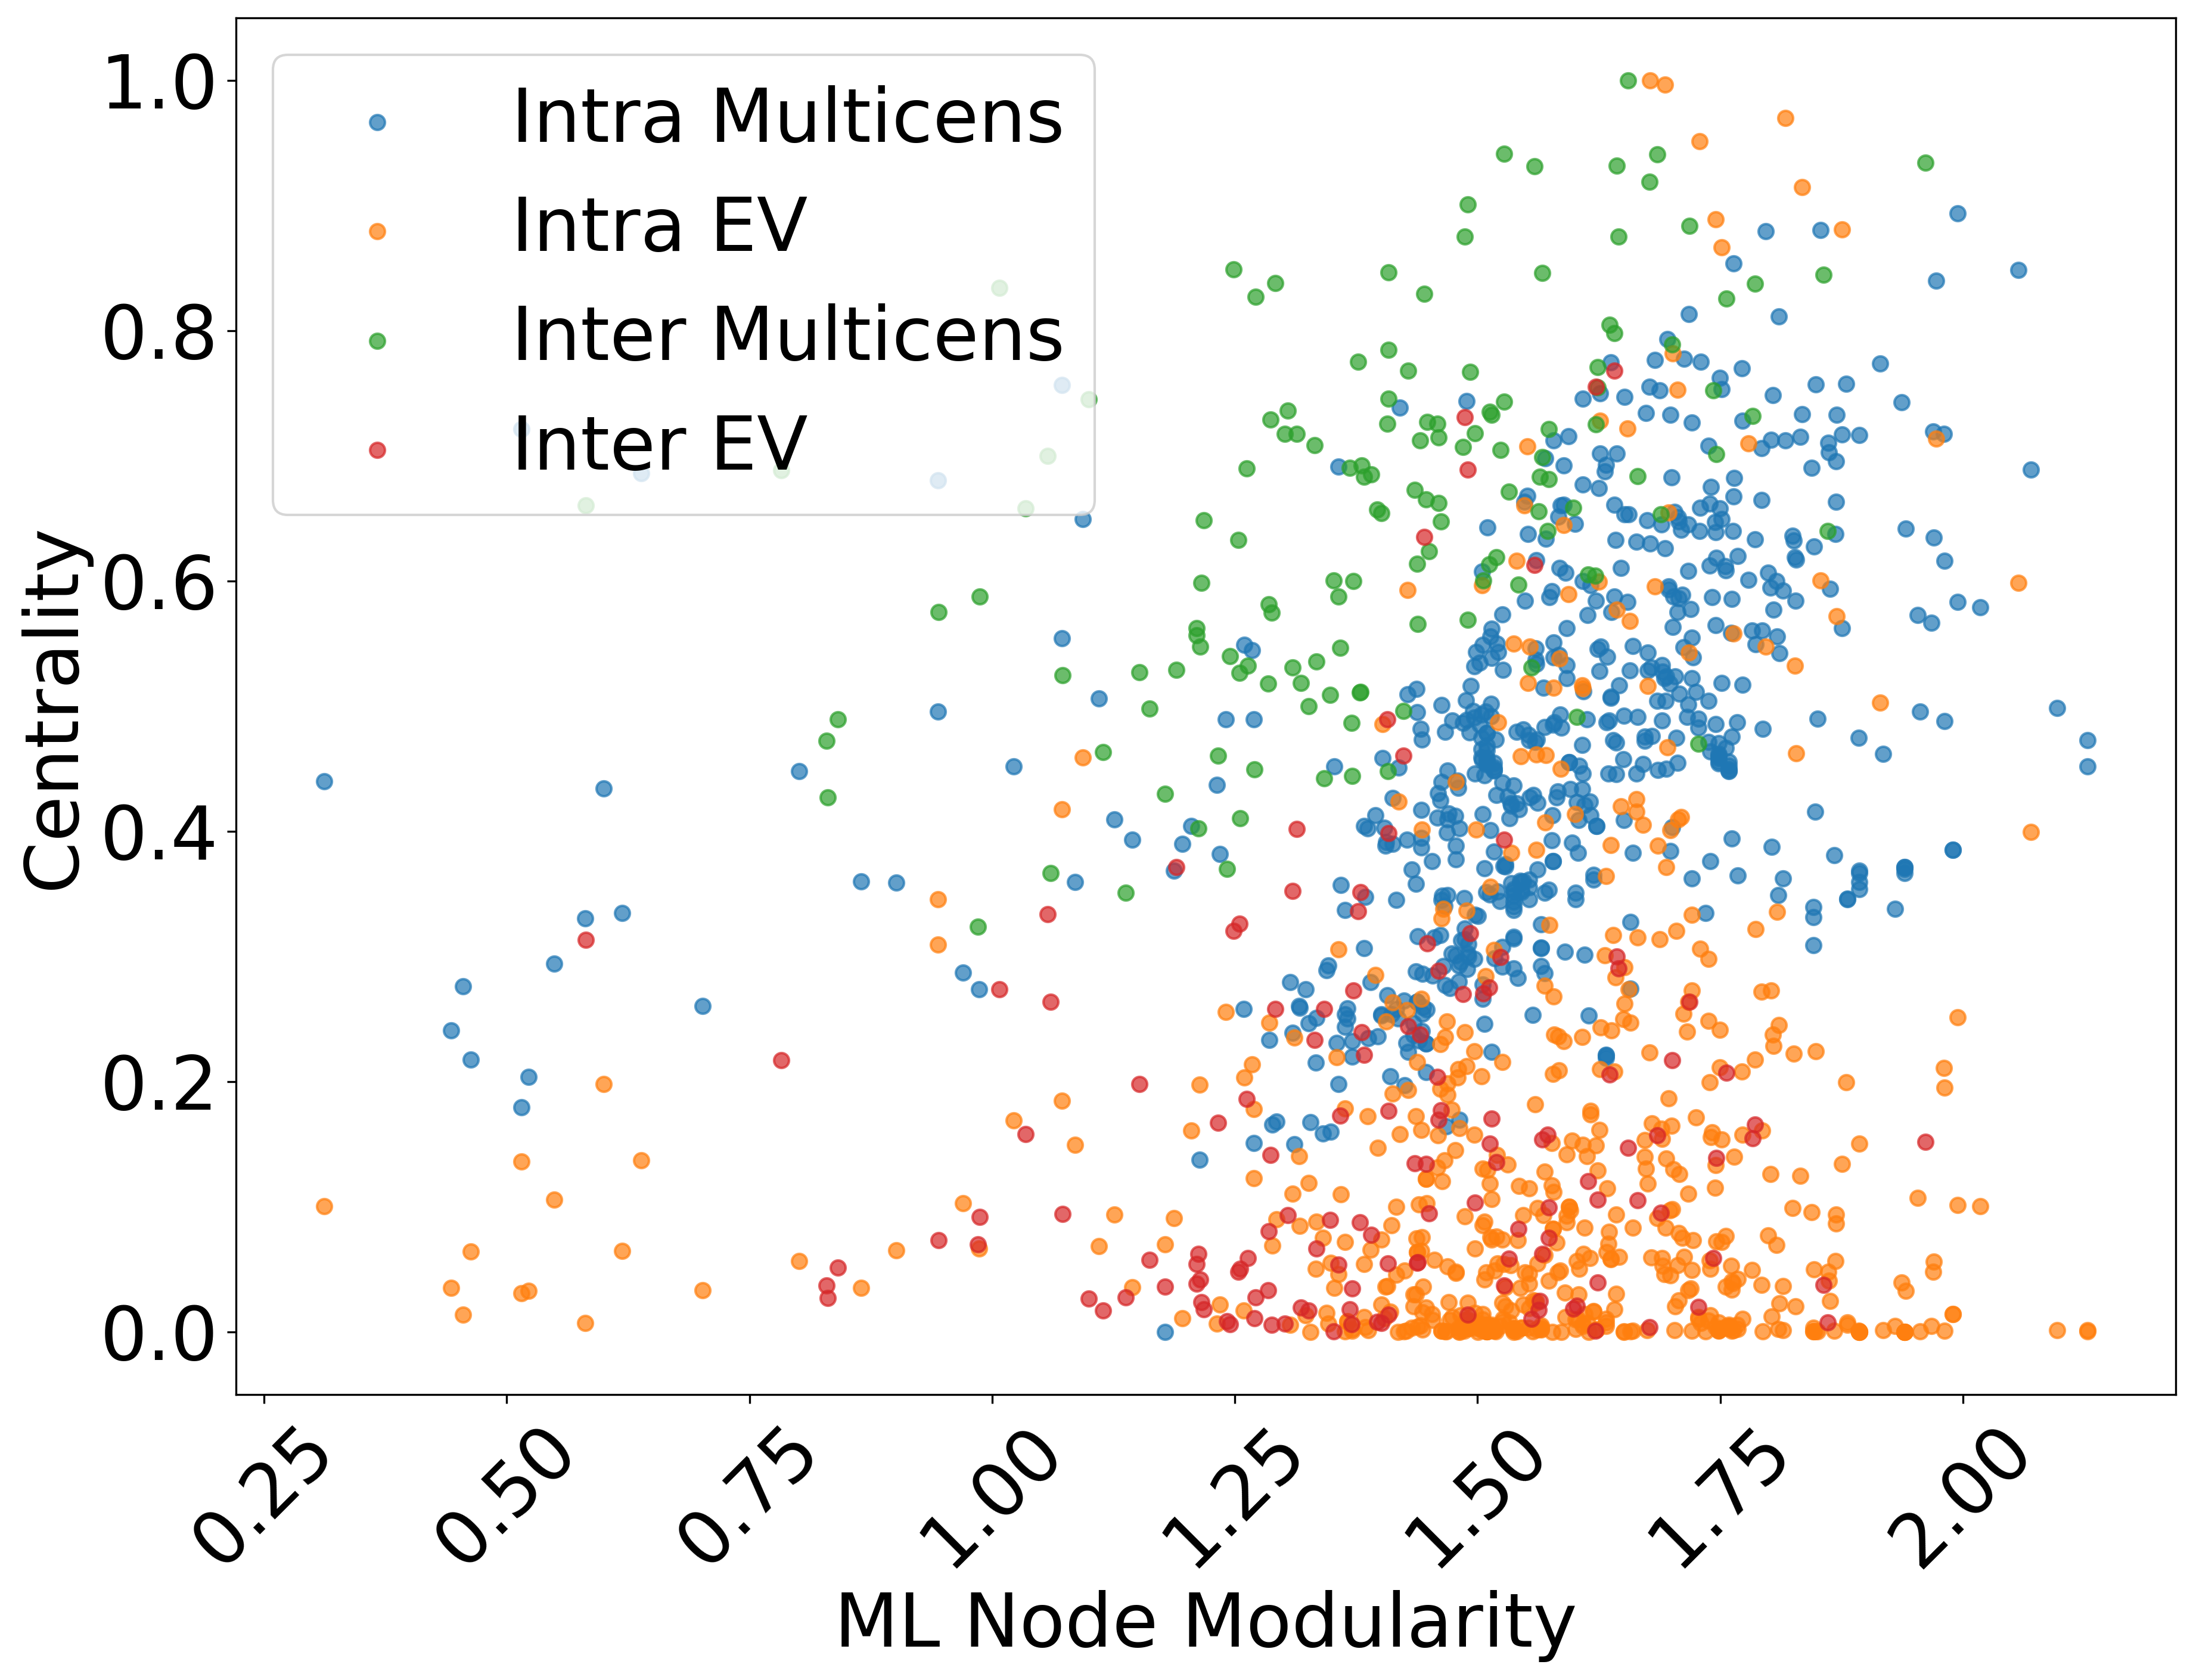
\includegraphics[width=\textwidth]{figs/fig5.png}
		\subcaption{}
	\end{minipage}
	\hspace{0.5cm}
	\begin{minipage}[b]{0.25\linewidth}
		\centering
		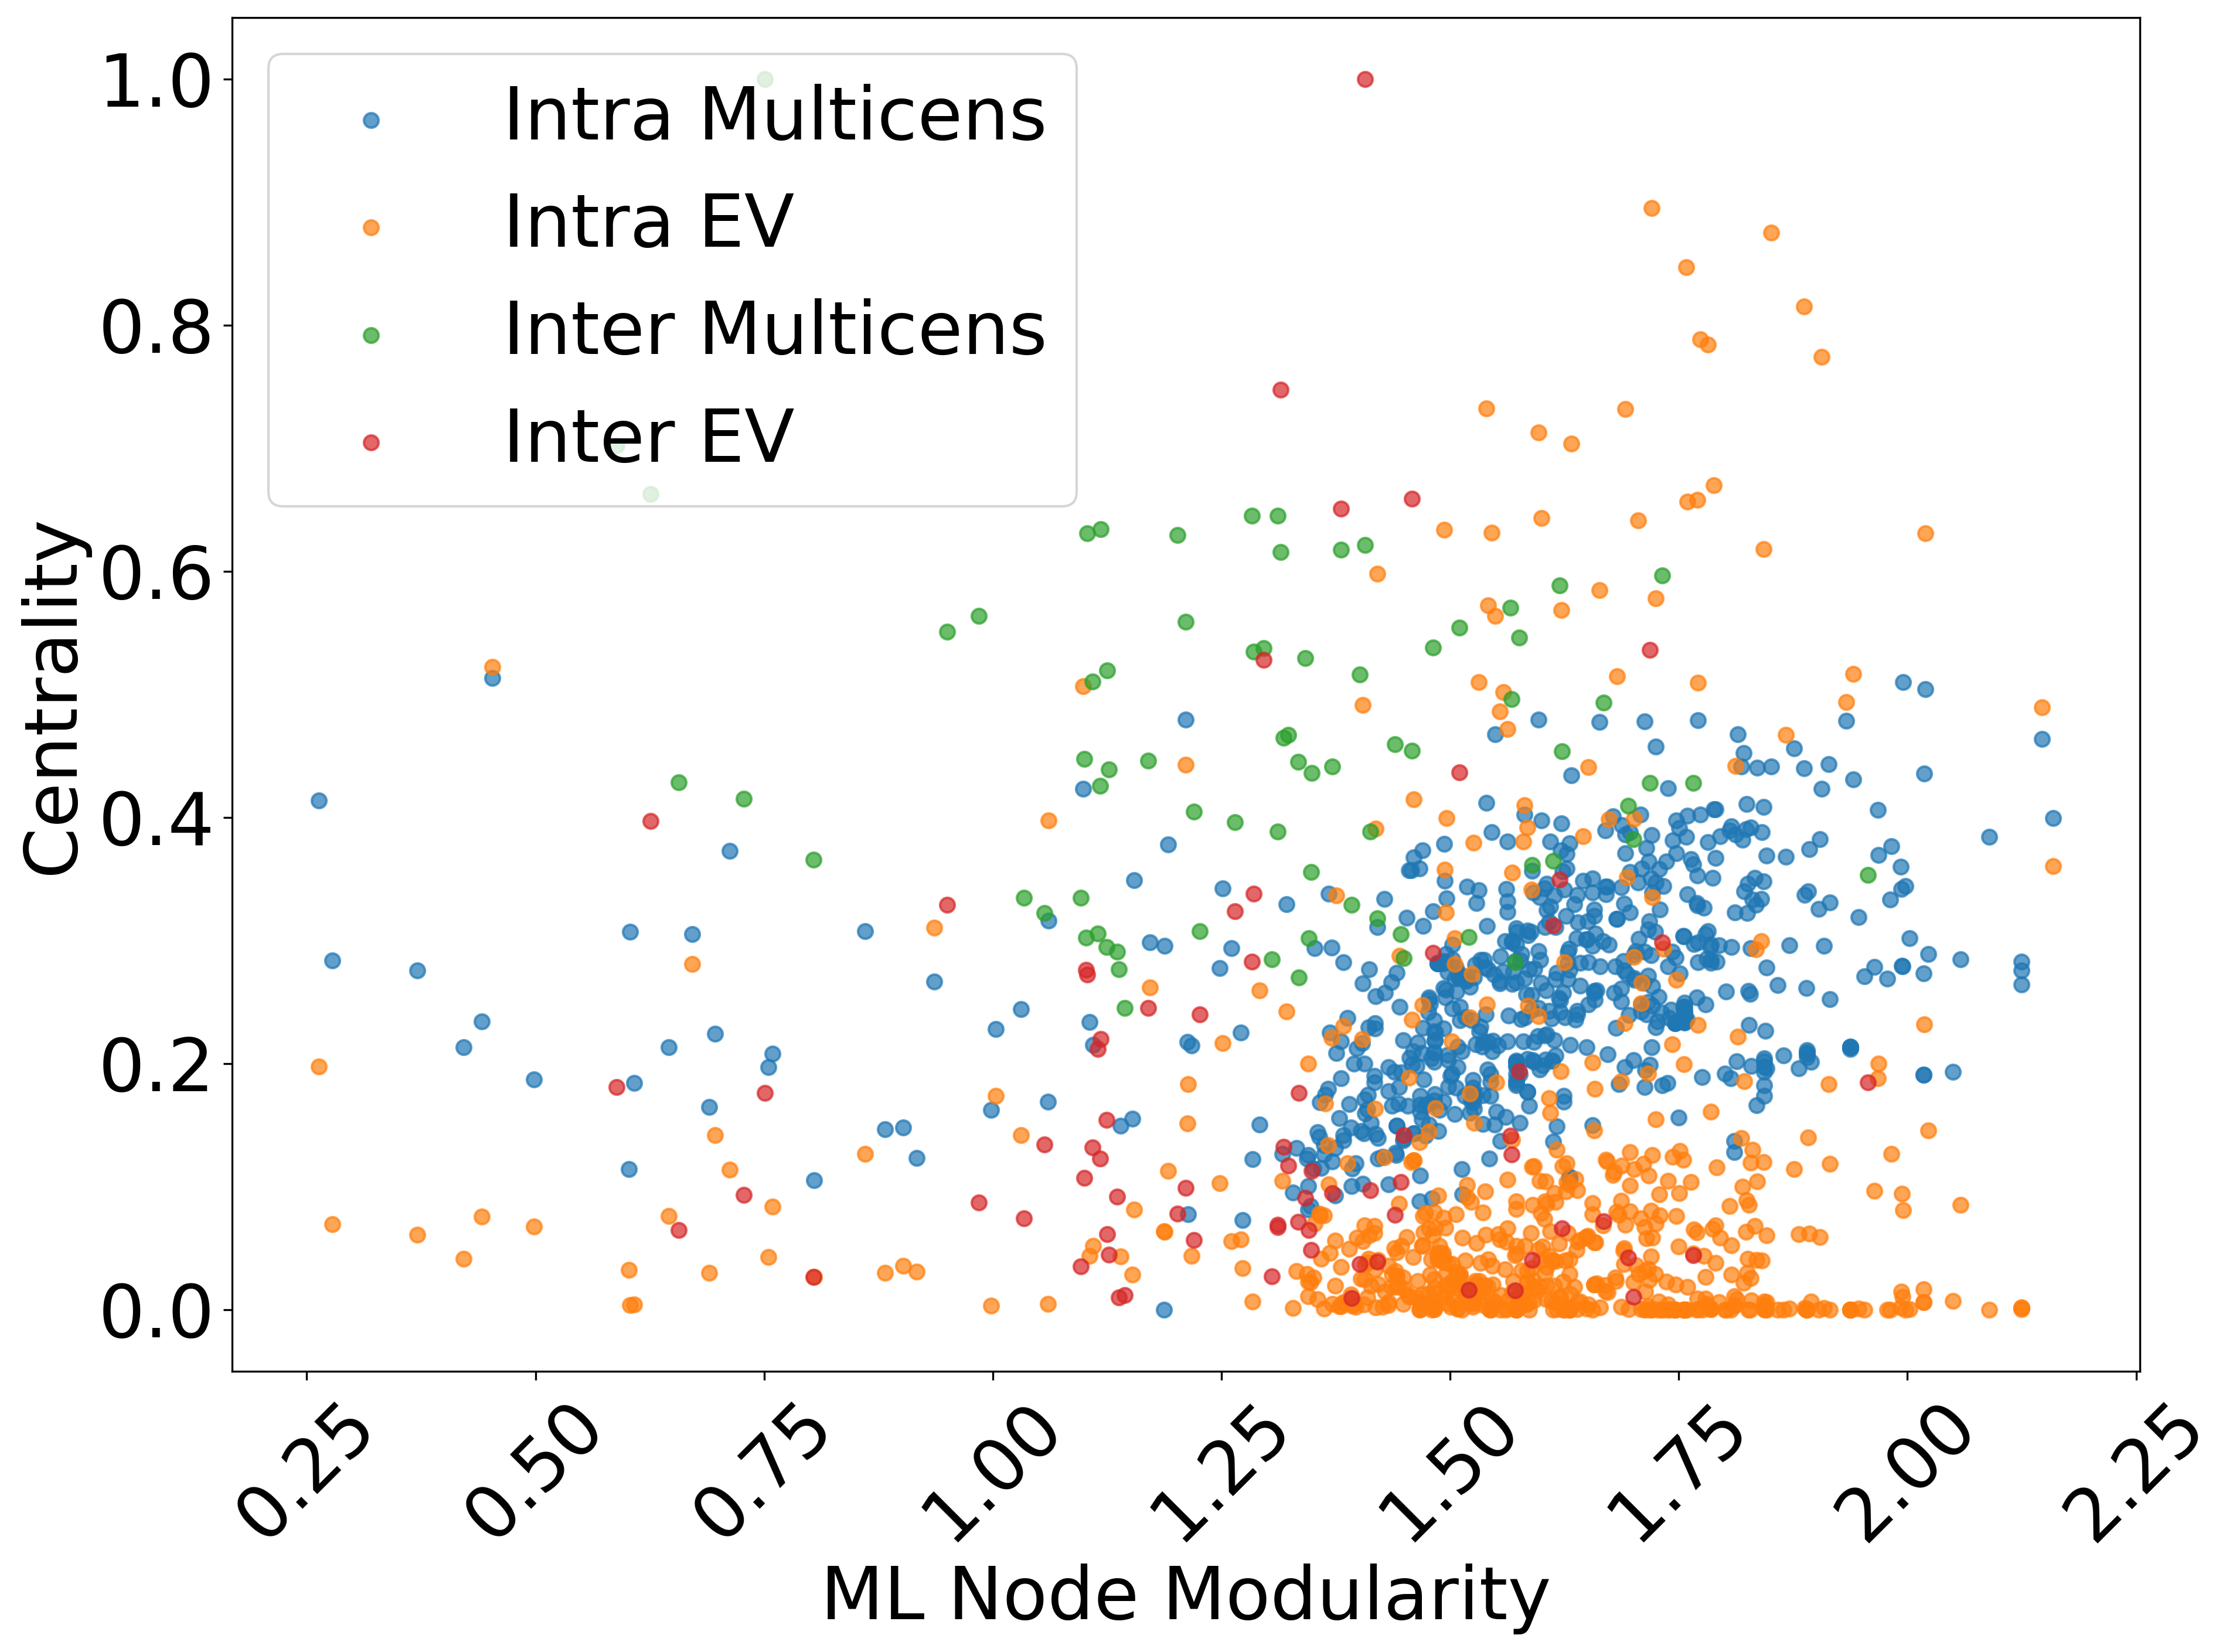
\includegraphics[width=\textwidth]{figs/fig6.png}
		\subcaption{}
	\end{minipage}
	
	\vspace{0.5cm}
	
	\begin{minipage}[b]{0.25\linewidth}
		\centering
		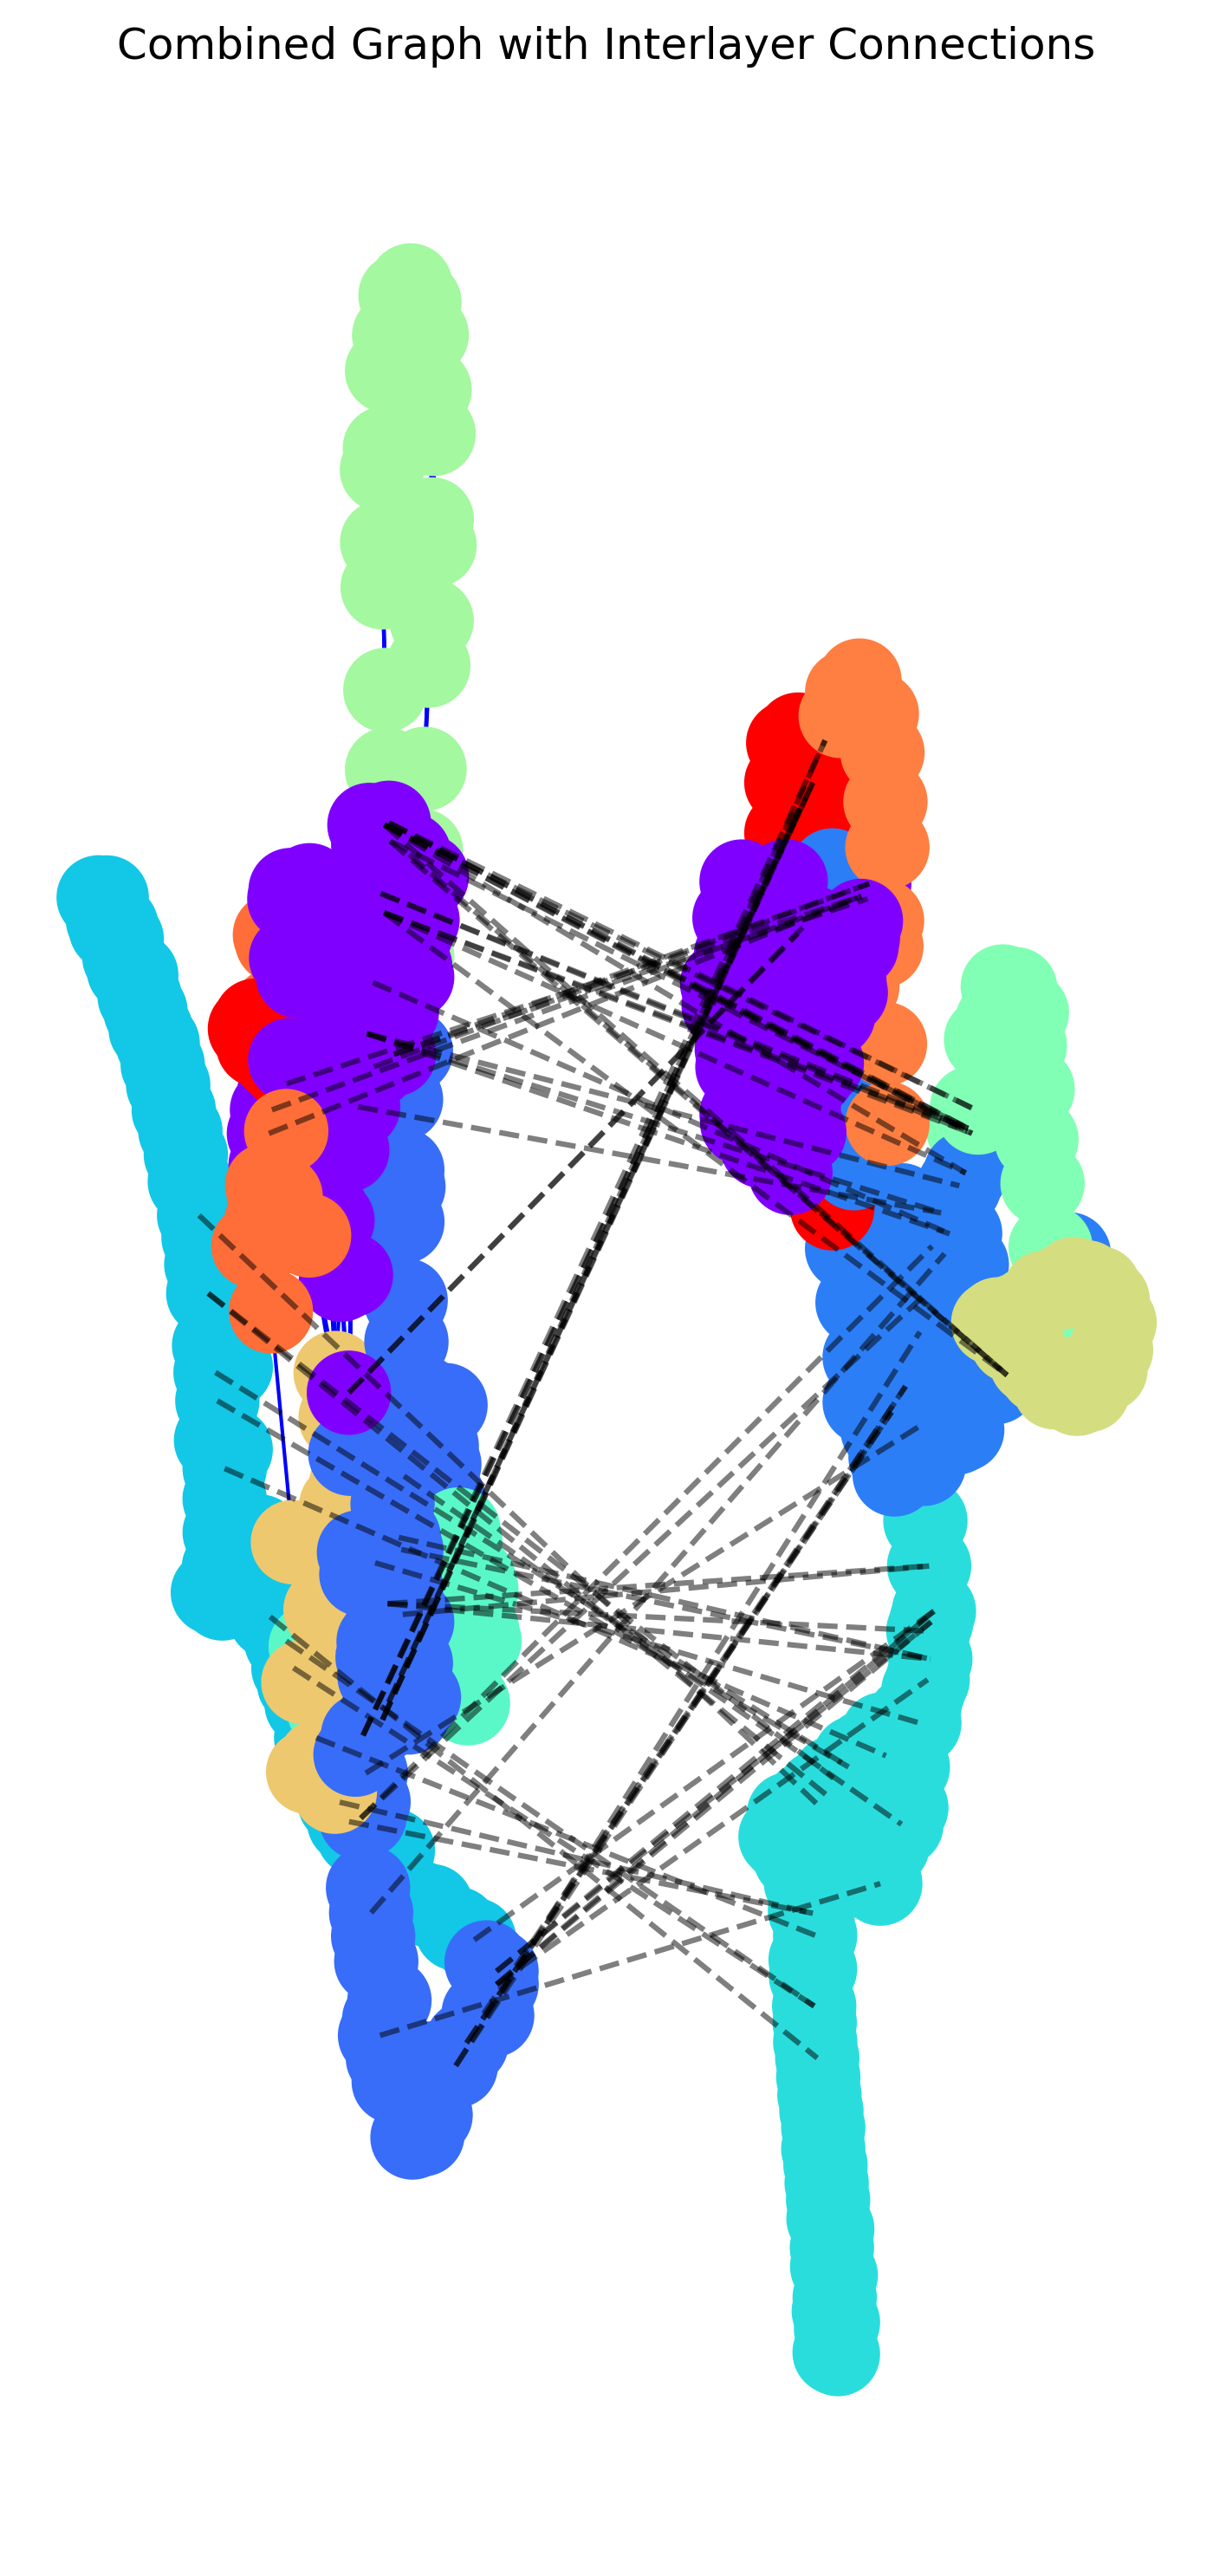
\includegraphics[width=\textwidth]{figs/fig7.png}
		\subcaption{}
	\end{minipage}
	\hspace{0.5cm}
	\begin{minipage}[b]{0.25\linewidth}
		\centering
		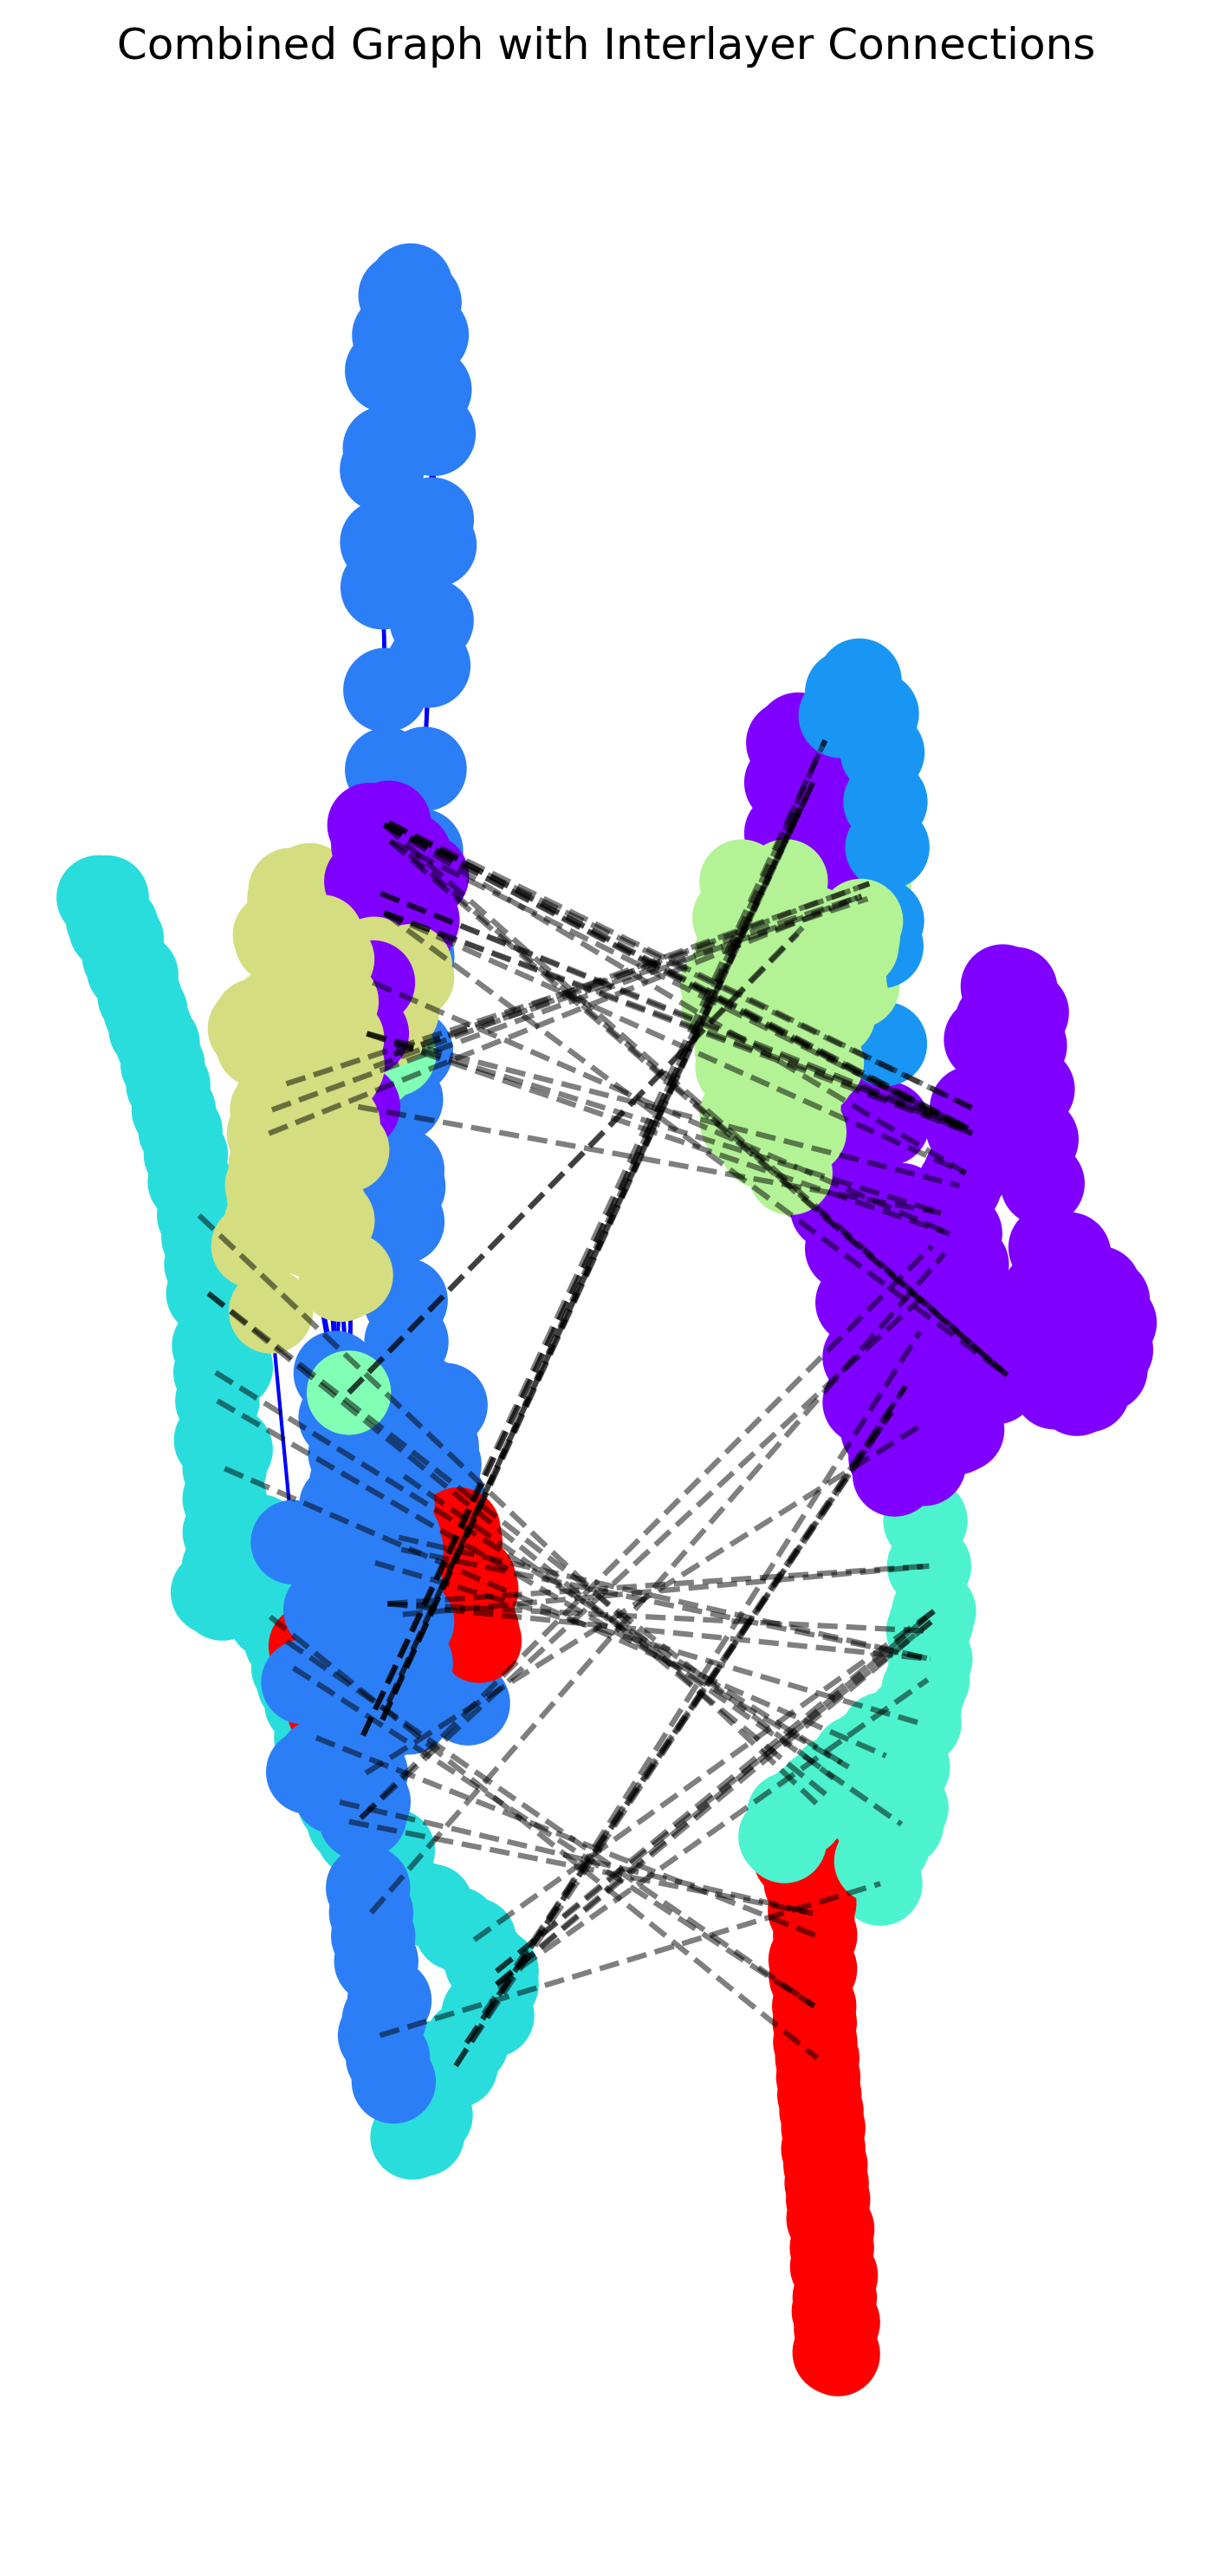
\includegraphics[width=\textwidth]{figs/fig8.png}
		\subcaption{}
	\end{minipage}
	\caption{(a) Node modularity vs. Centrality; (b) Node modularity vs. Eigen-vector centrality; (c) Inter vs intra layer modularity of single and multilayer centralities; Inter vs intra layer modularity of single and multilayer centralities using (d) random interface 1, (e) random interface 2 (all pairs shortest path distribution chosen from the original, (f) random interface 3 (all pairs shortest path distribution as close as possible with the original; (g) Node modularity vs. Centrality. (h) Inter-layer modularity depends on intra-layer structures \label{fig:modvcen}}
\end{figure}

\section*{Motivation}
To demonstrate differences in how single-layer and multi-layer centrality measures capture network characteristics, we begin by using modularity to compare intrachain and interchain dynamics. 

Modularity captures the underlying structure of the network. It measures how strong a network is with respect to being broken down into communities~\cite{newman2006mod} or subsets of nodes. A high value typically indicates dense graph structure within communities and sparse connections between communities.  For an individual node, modularity is not usually computed in isolation but in the context of its community. To understand the presence of dependence of interchain on intrachain structure, we first define node level {\it greedy} modularity $Q_i$ for node $i$ as follows~\cite{newman2006mod,newman2006nw,reichardt2006commu,newman2004commu,newman2012nws,newman2004greedy}:
\begin{equation}
\label{eqn1}
Q_i = \frac{1}{2m} \sum_{i,j} \left[A_{ij}^{Intra} - \frac{k_i k_j}{2m} \right] \delta(c_i, c_j)
\end{equation}
where $m$ is total number of edges in the graph, $A_{i,j}^{Intra}$ is the intra-layer connection between $i$, $j$, $k_i$ is degree of node $i$, $k_j$ is degree of node $j$, $\delta(c_i, c_i)$ is 1 if nodes $i$ and $j$ are in the same community and 0 otherwise. 

Based on the above definition, nodes with low modularity should have low centrality because centrality captures node's local and global properties while modularity reflects a node's involvement in communities. If a node is not involved in strongly knit sub-networks, such a node should not be central (per degree, betweenness, eigen vector, etc.). Additionally, if indeed interchain structures are dependent on intrachain networks, then node level modularity might have some discernable correlation with multilayer centralities as both capture a node's participation in communities. Single layer centrality measures such as Eigen vector centrality, while capturing a node's influence in local and global network properties, do not particularly measure participation in communities--which may be necessary to quantify its role in interlayer structures, as interlayer structures are much sparser than intralayer structures. Figure~\ref{fig:modvcen} (a) shows that node modularity contribution is correlated with MultiCens (a multilayer centrality measure) values, and low centrality values (regardless of whether it is single layer or multi-layer) means low modularity values. 

\begin{figure}[h!]
	\centering
	\begin{minipage}[b]{0.44\linewidth}
		\centering
		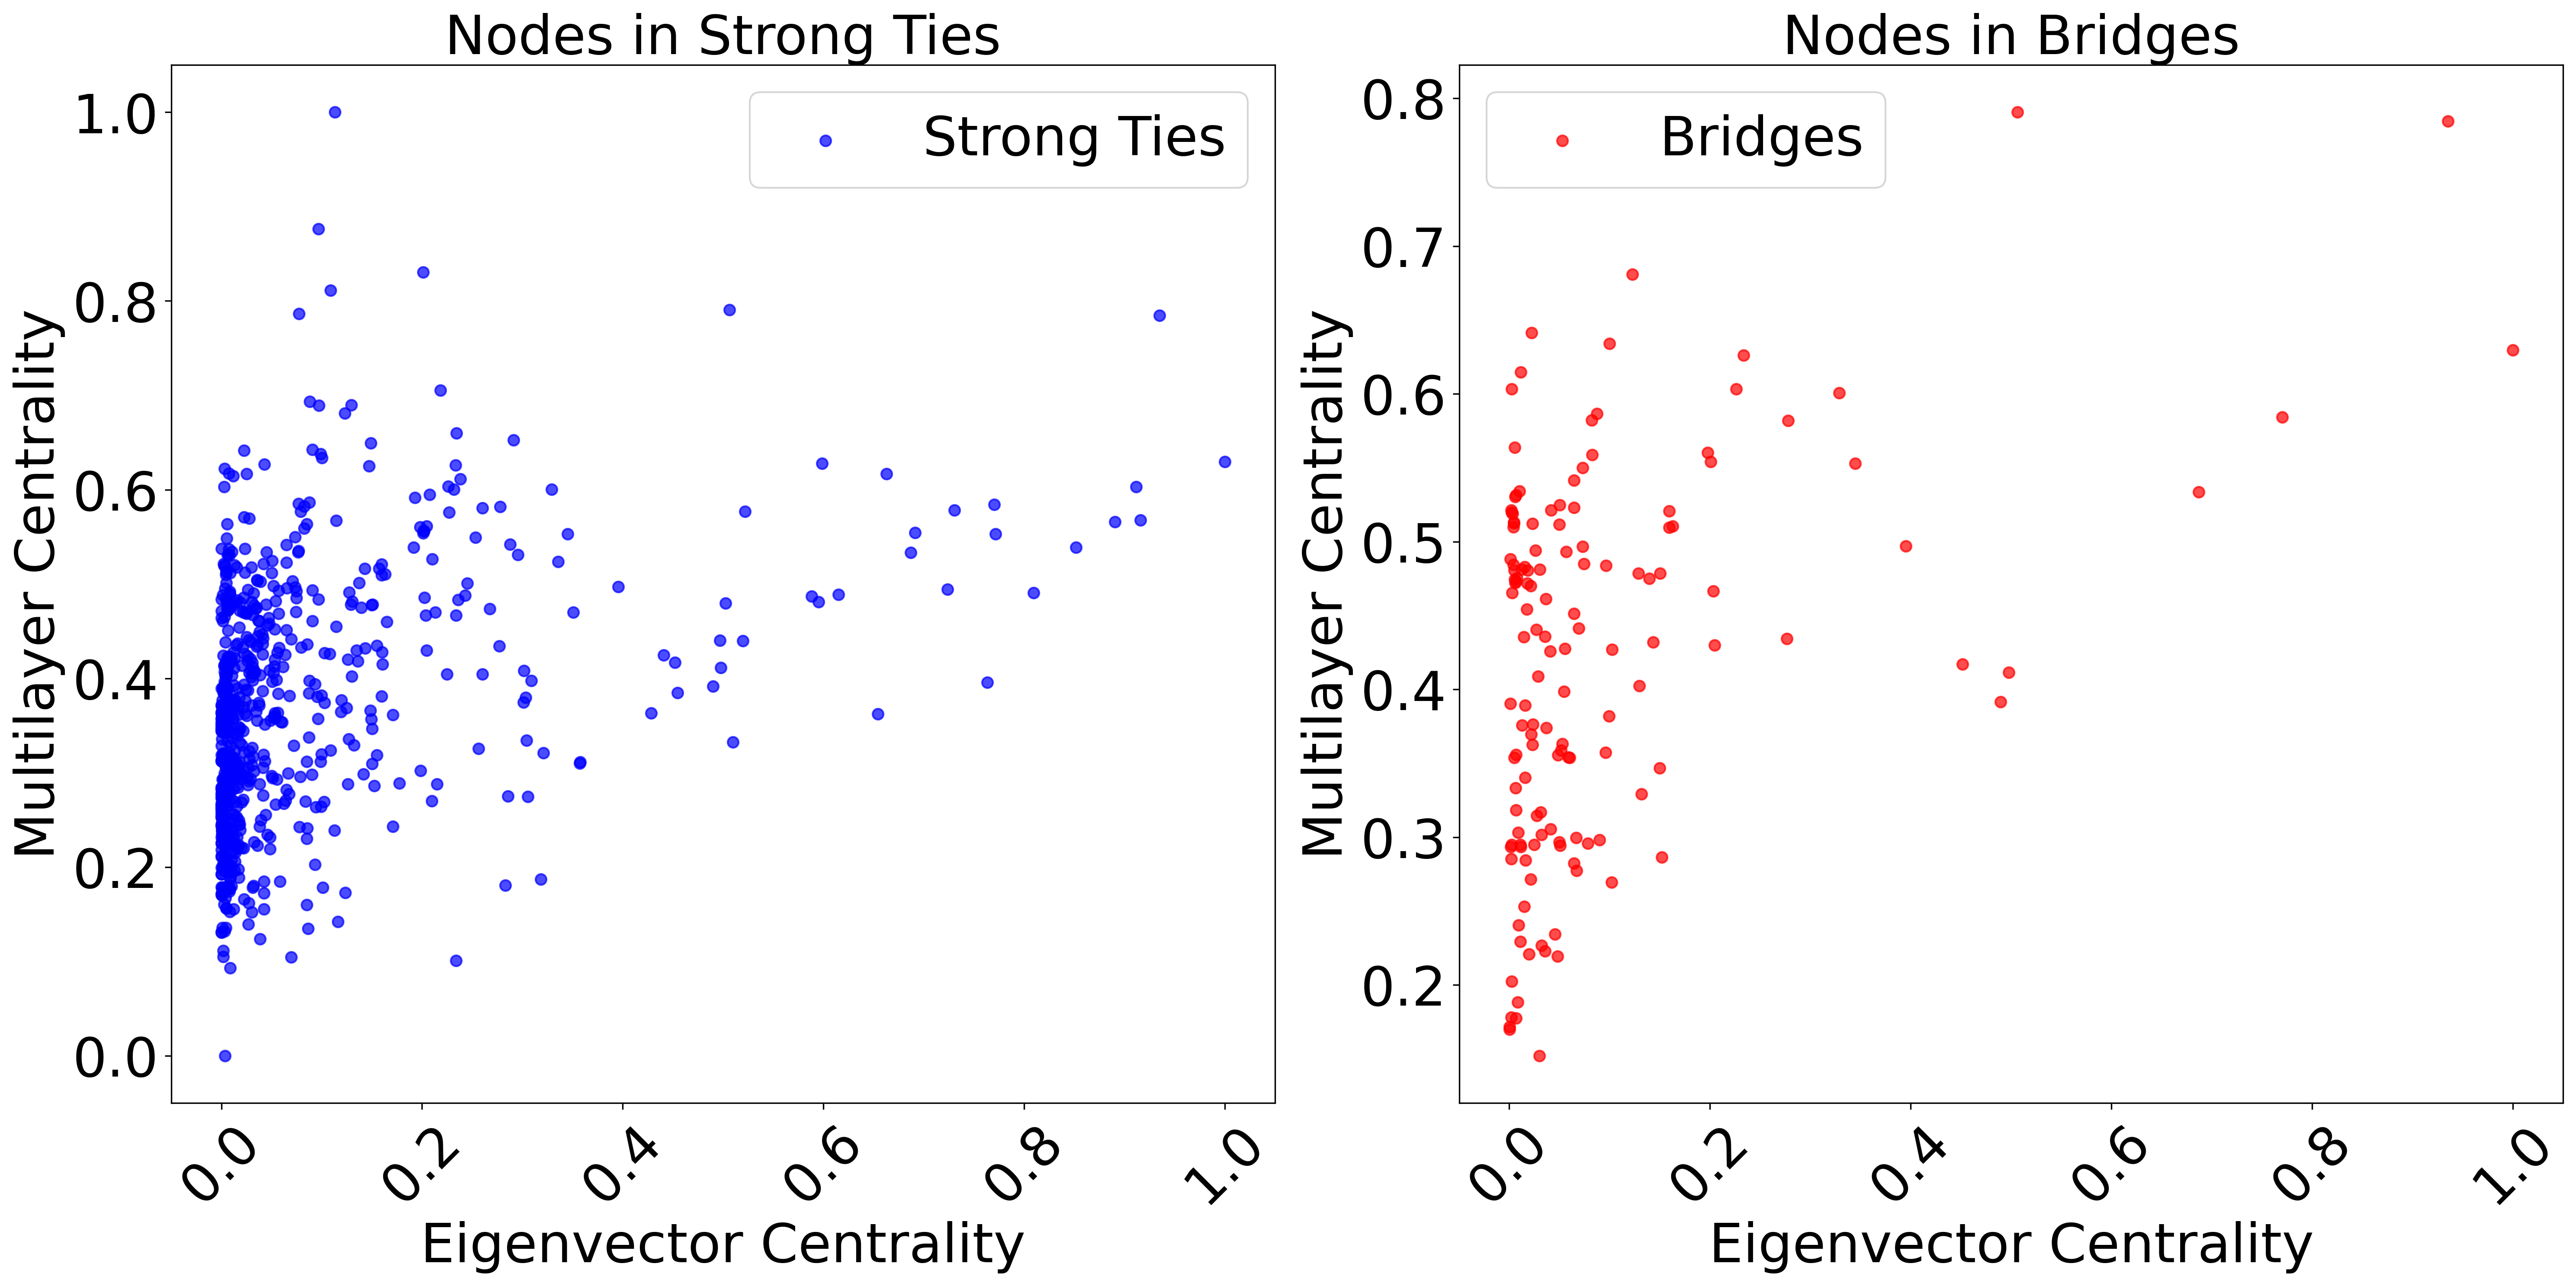
\includegraphics[width=\textwidth]{figs/fig9.png}
		\subcaption{}
	\end{minipage}
	\hspace{0.5cm}
	\begin{minipage}[b]{0.44\linewidth}
		\centering
		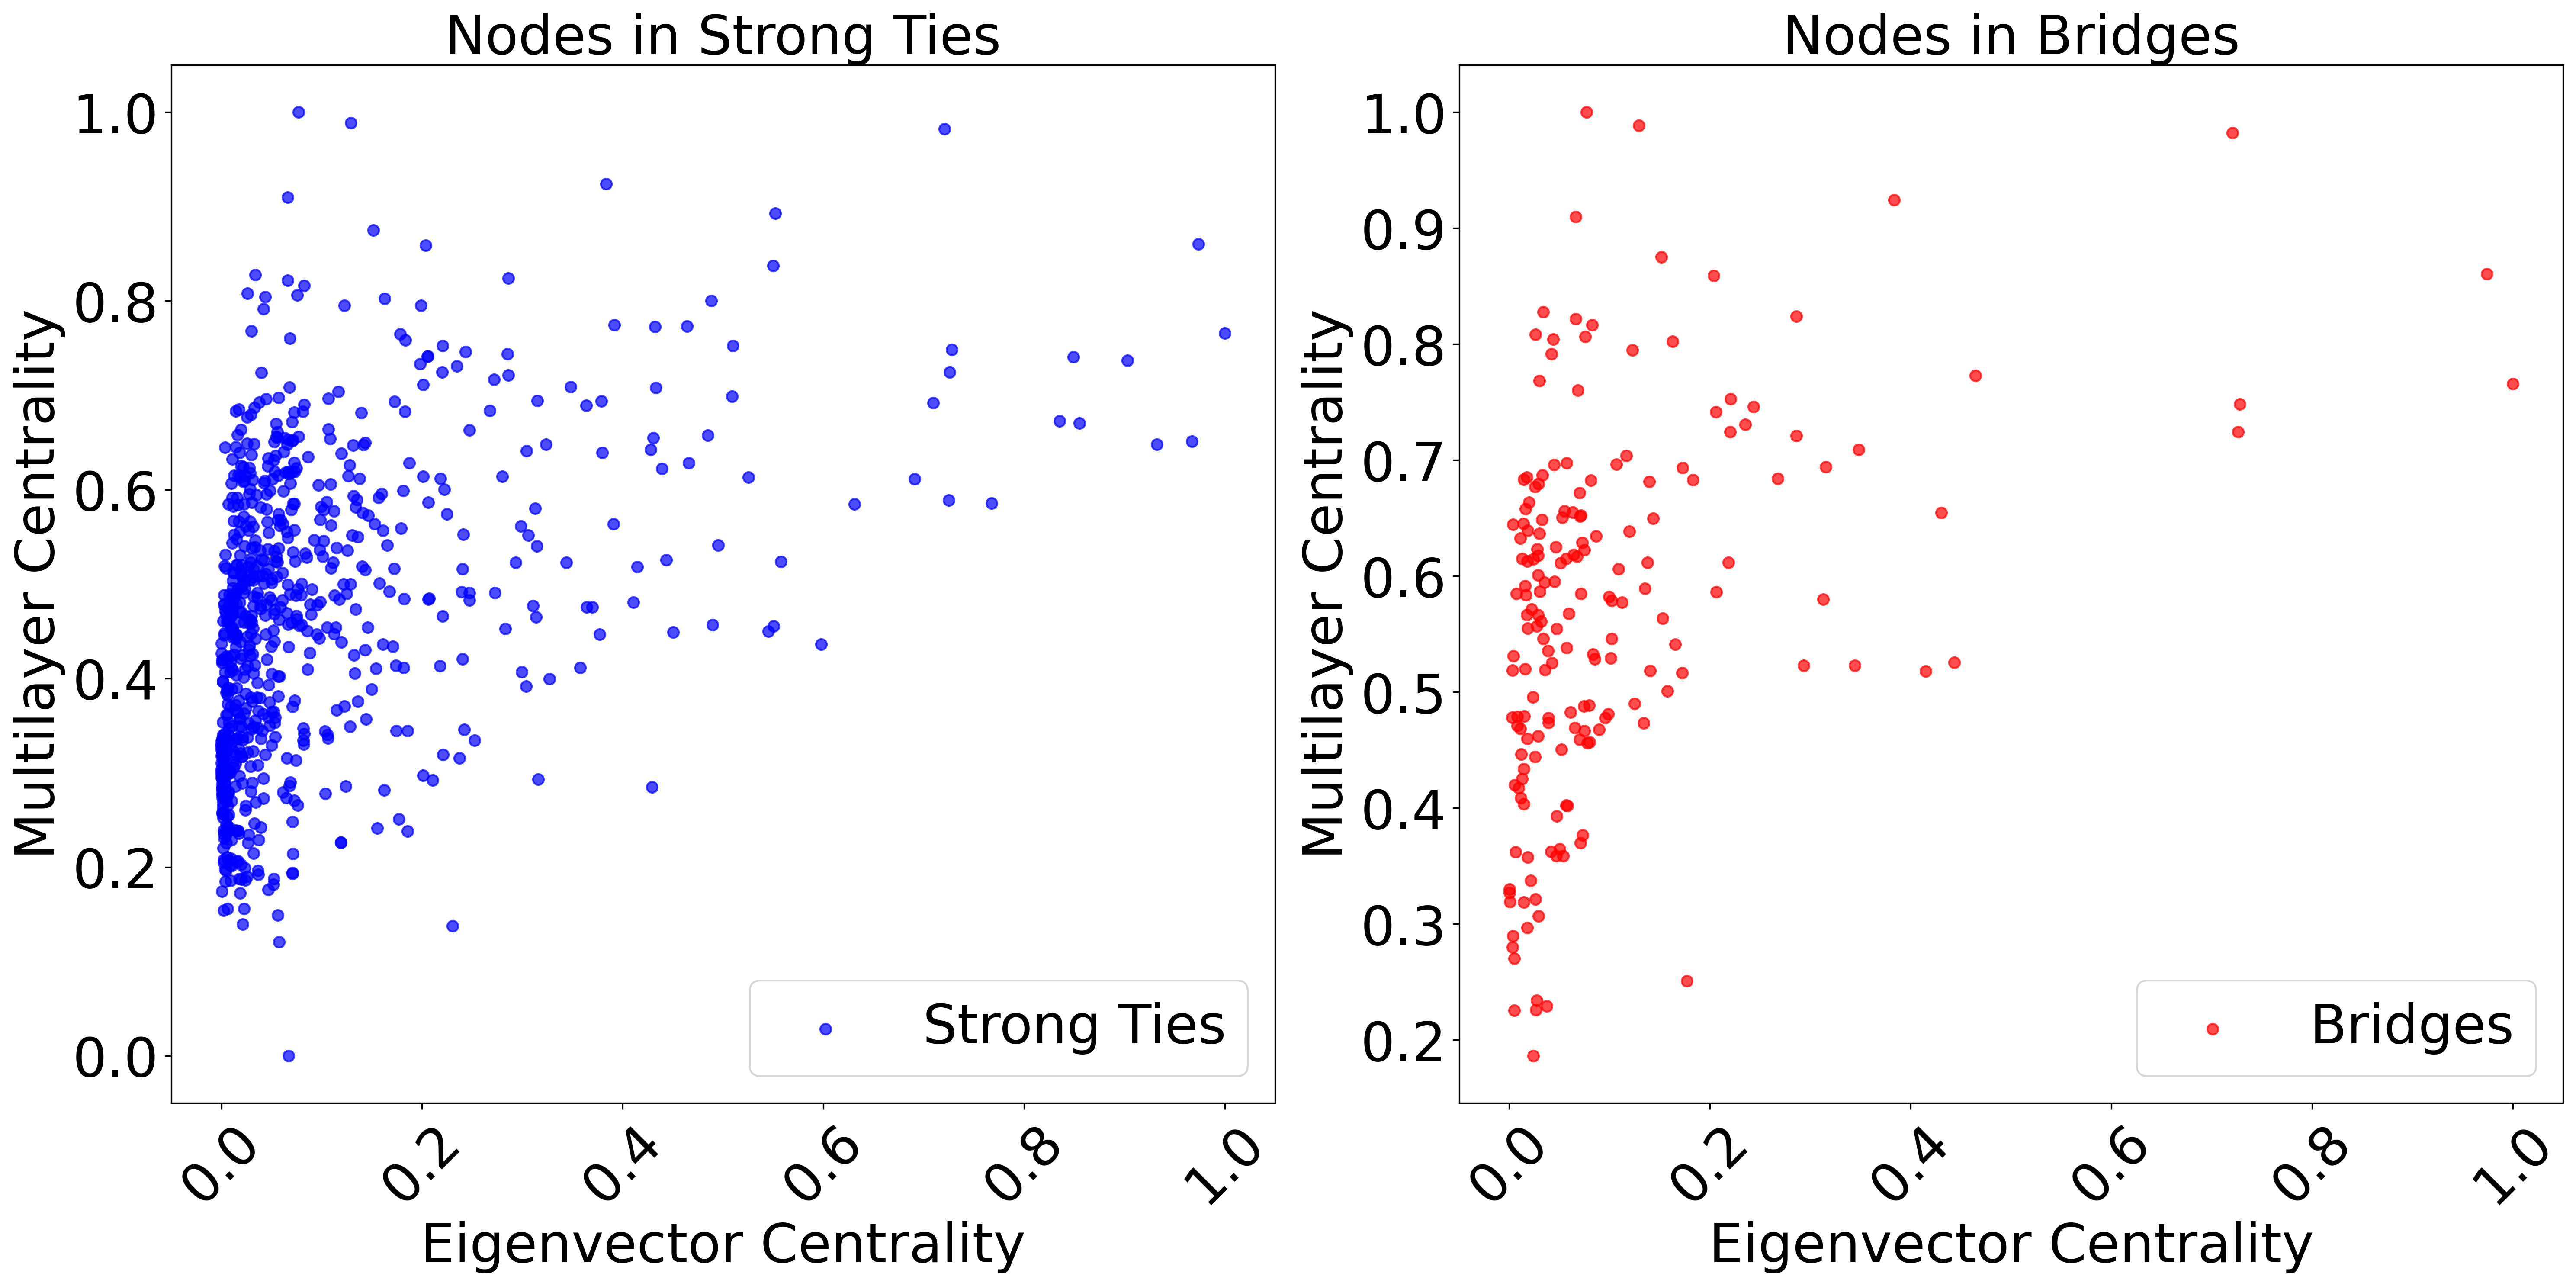
\includegraphics[width=\textwidth]{figs/fig10.png}
		\subcaption{}
	\end{minipage}
	\caption{(a) Eigen vector vs multicens centrality of strong ties (on the left) and bridges (on the right). Eigen vector vs multicens centrality of strong ties (on the left) and bridges (on the right) for random interlayer configurations; (b) Random interface 1. \label{fig:ties1}}
\end{figure}

\begin{figure}[h!]
	\centering
	\begin{minipage}[b]{0.44\linewidth}
		\centering
		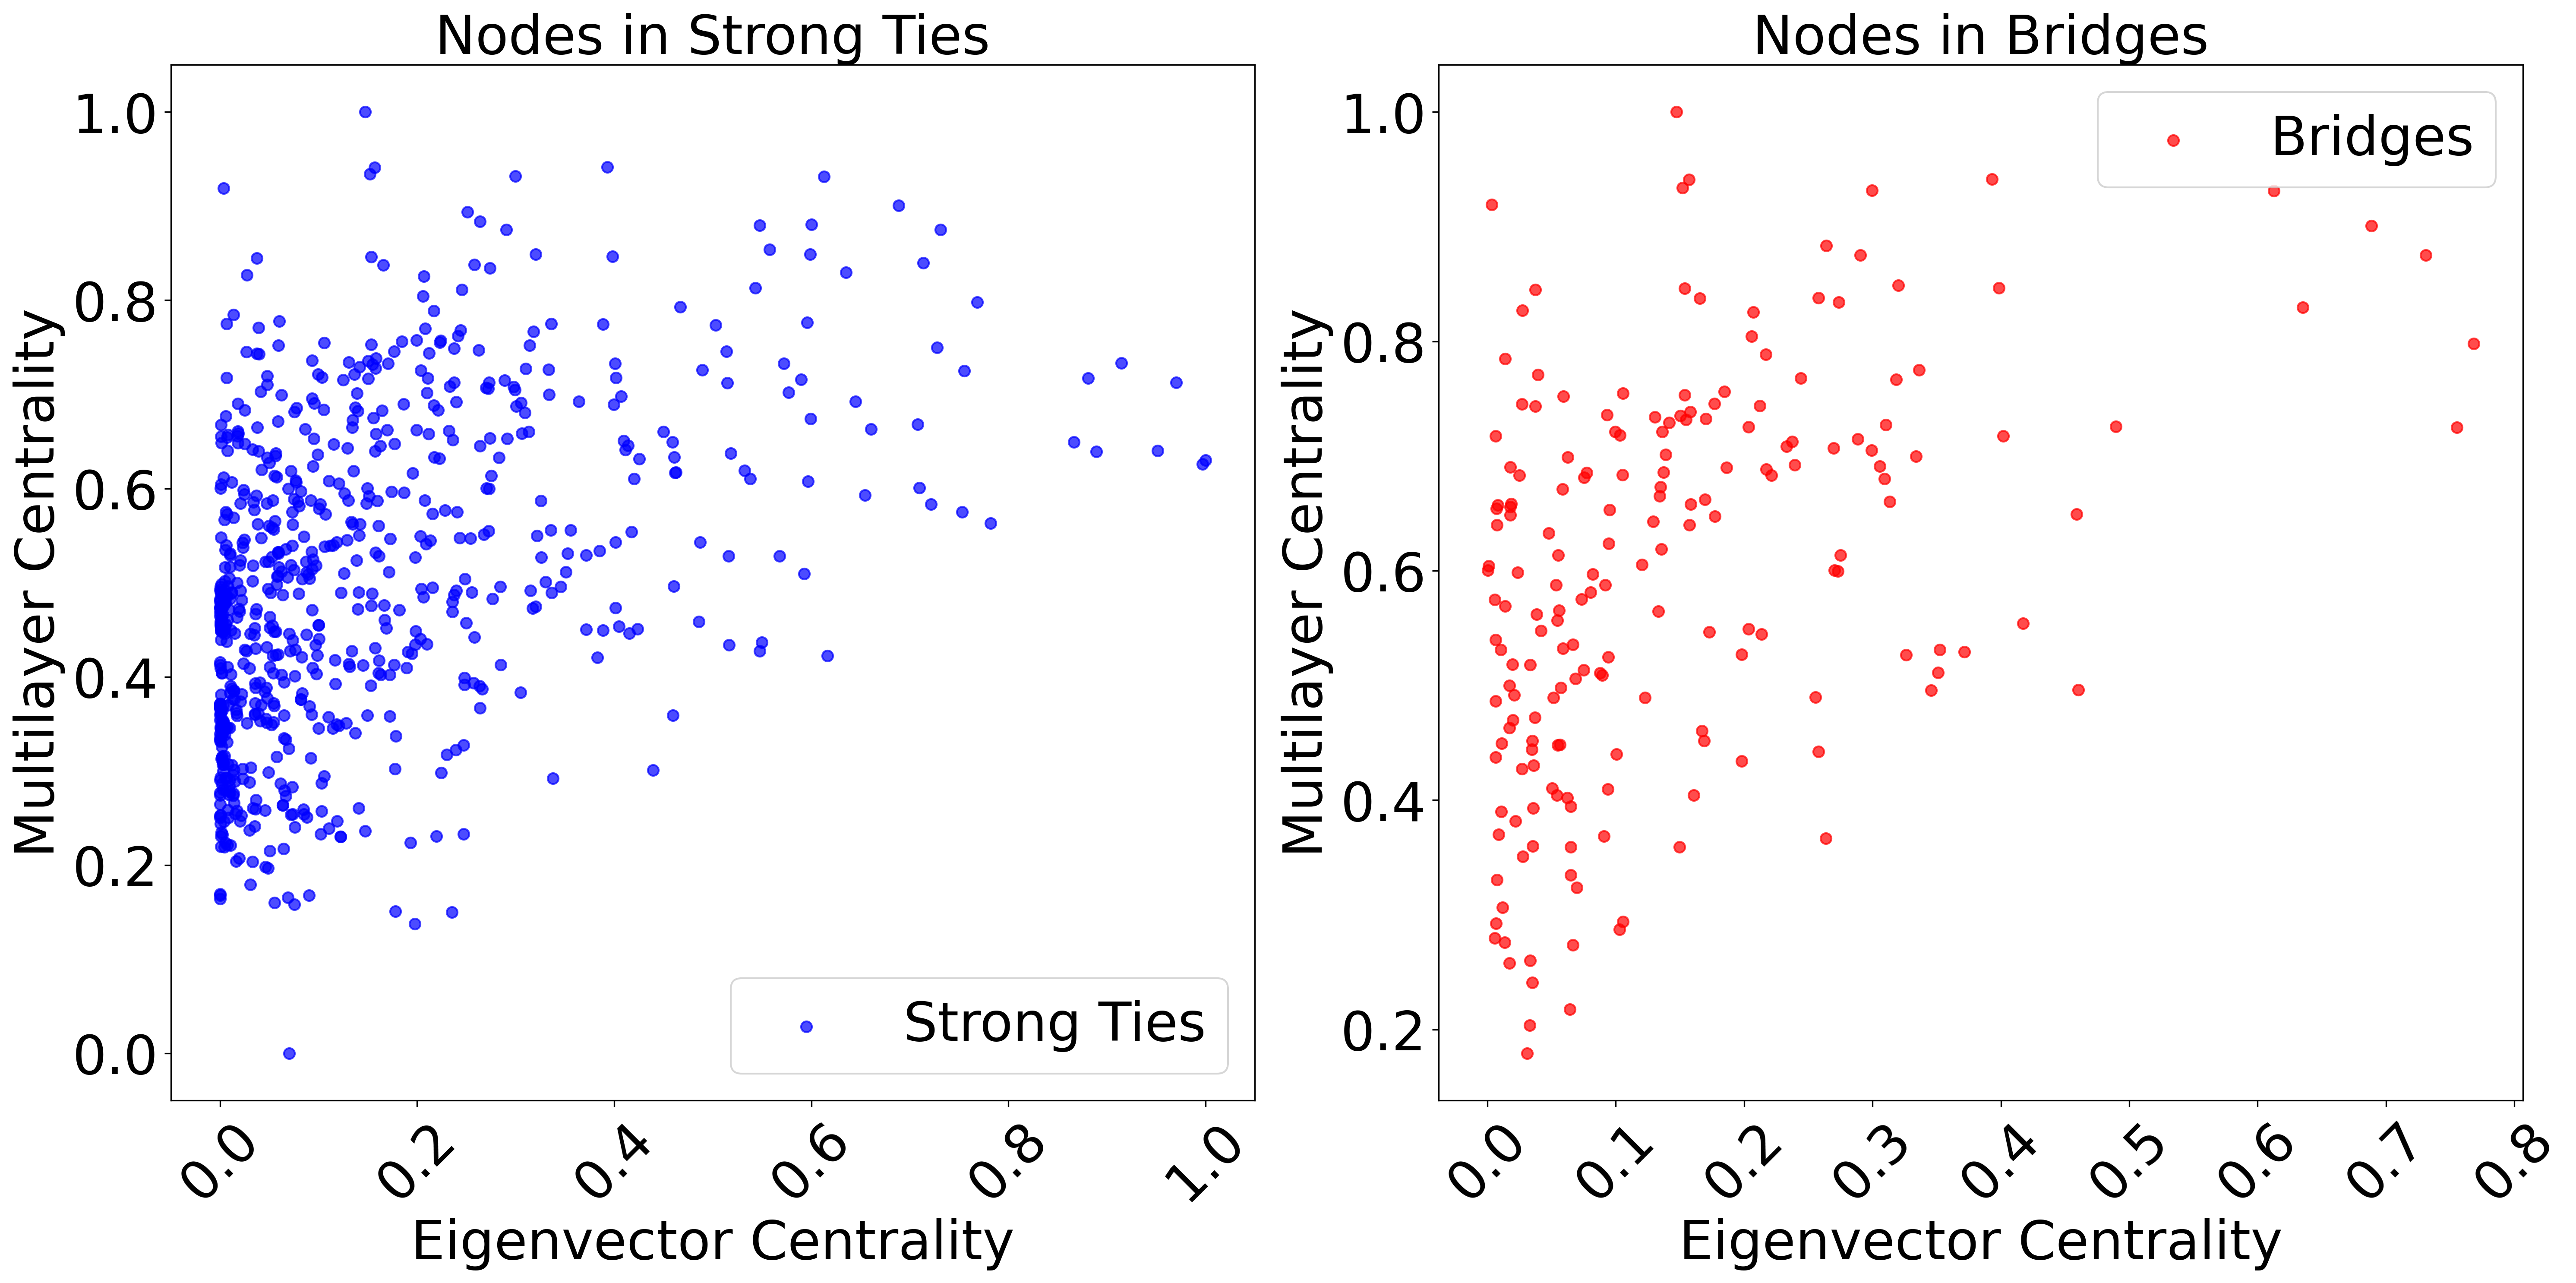
\includegraphics[width=\textwidth]{figs/fig11.png}
		\subcaption{}
	\end{minipage}
	\hspace{0.5cm}
	\begin{minipage}[b]{0.44\linewidth}
		\centering
		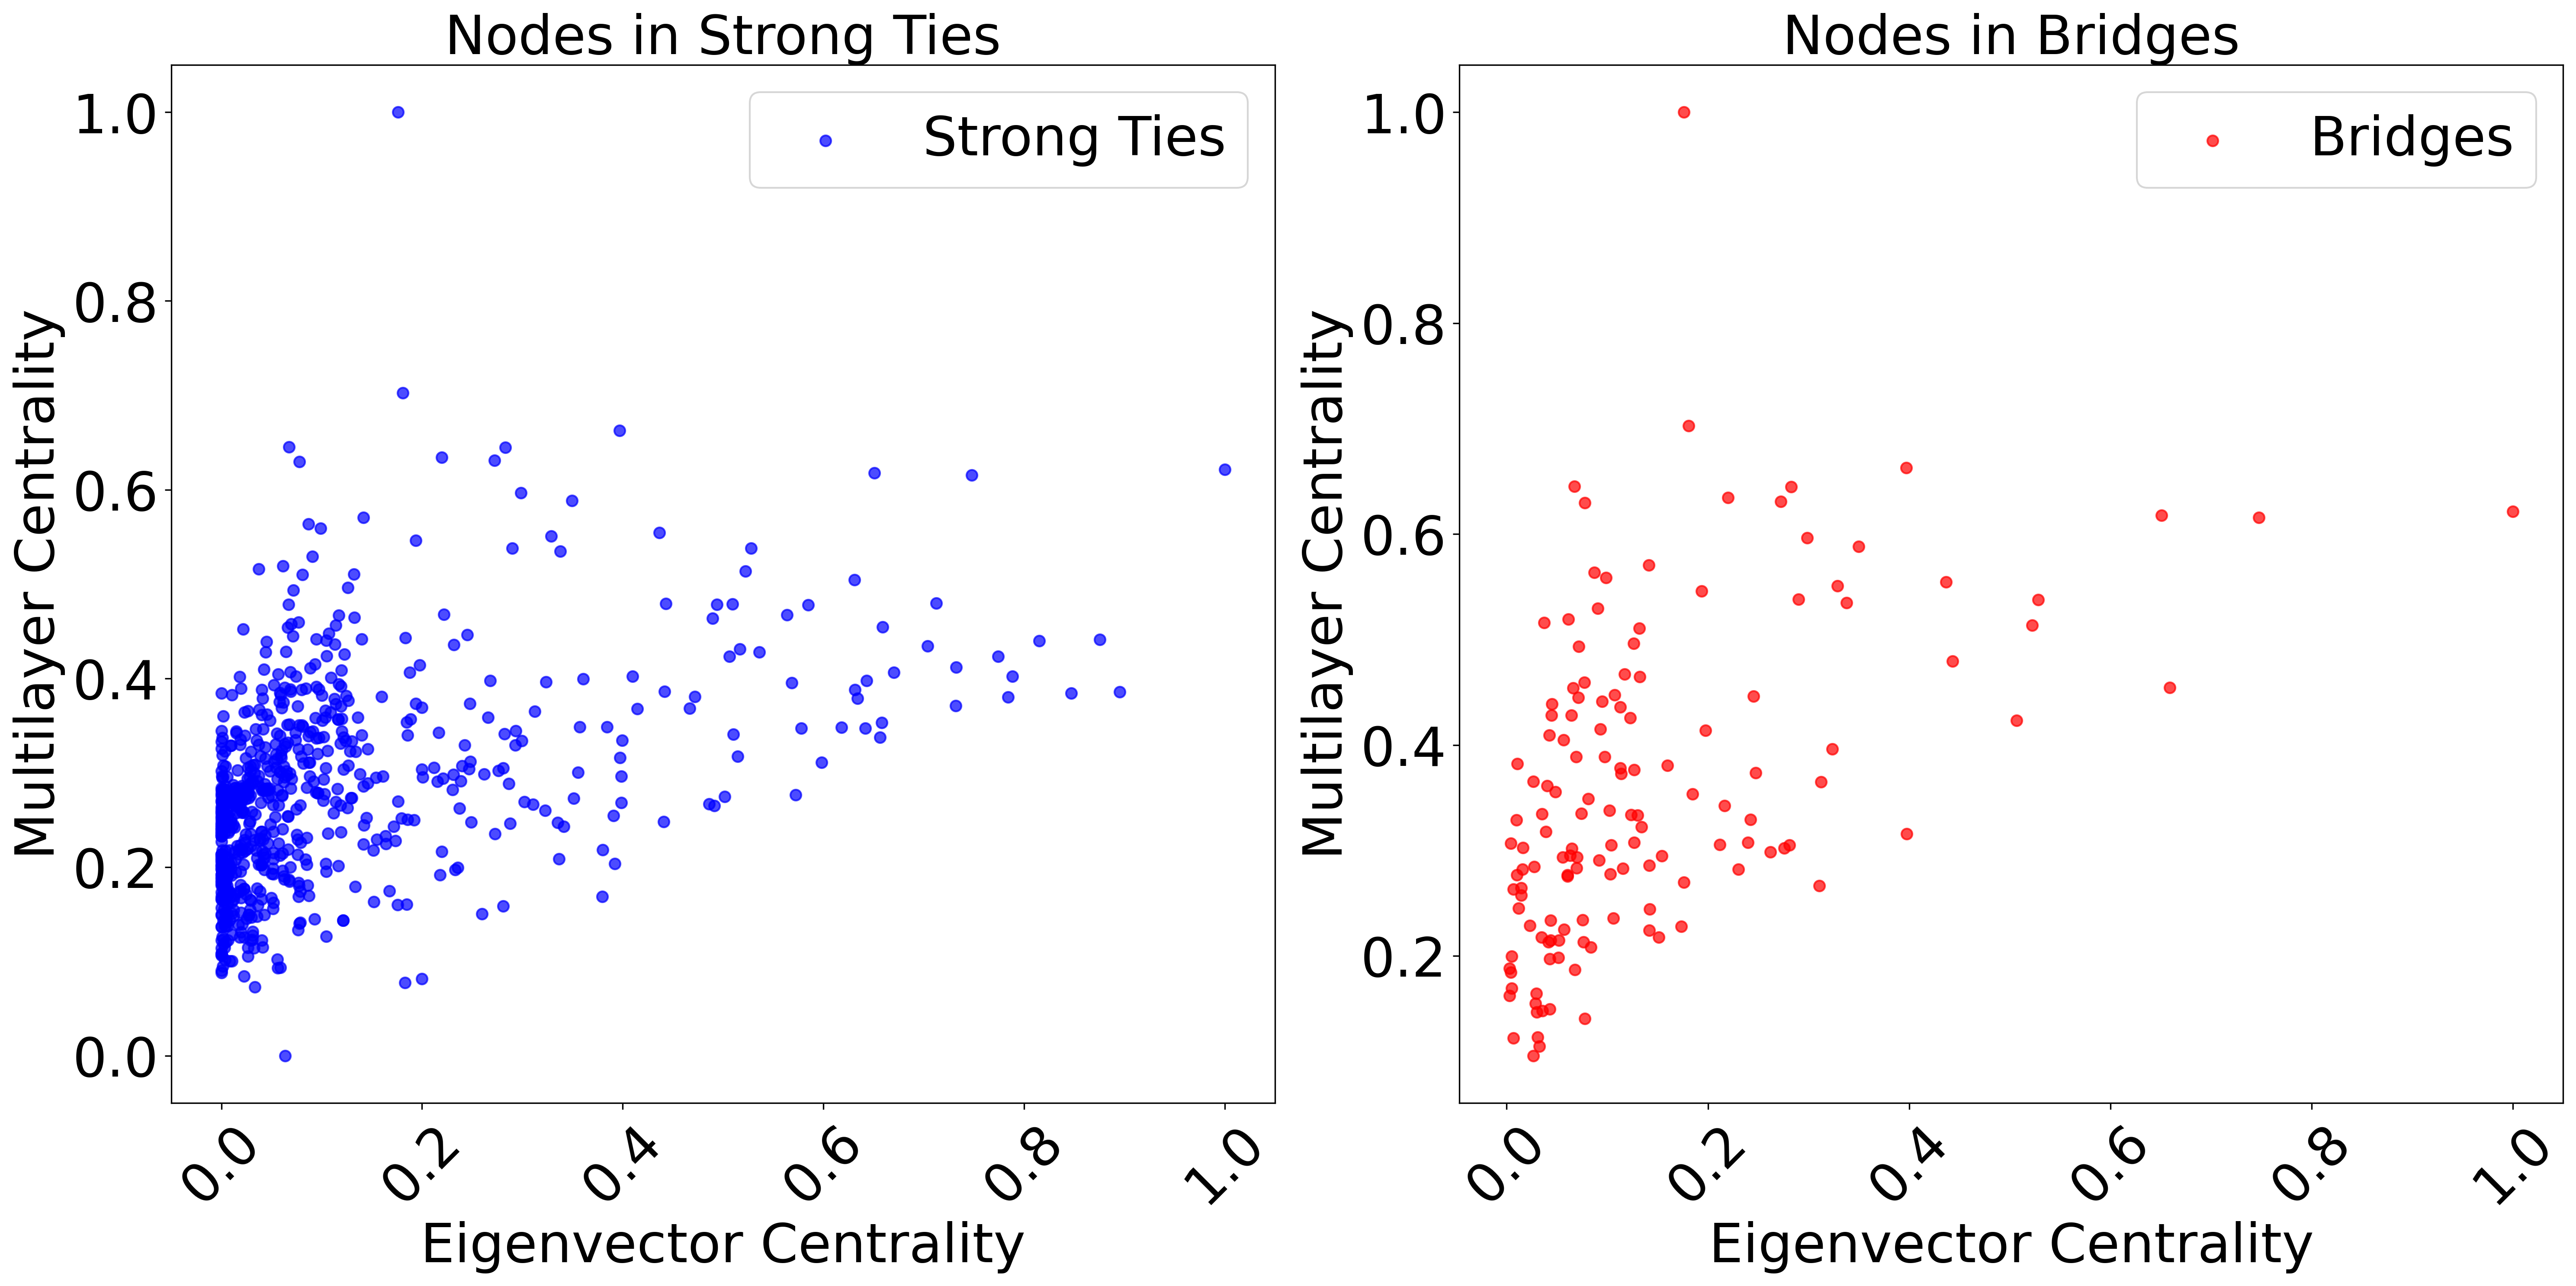
\includegraphics[width=\textwidth]{figs/fig12.png}
		\subcaption{}
	\end{minipage}
	\caption{Eigen vector vs multicens centrality of strong ties (on the left) and bridges (on the right) for random interlayer configurations; (a) Random interface 2; (a) Random interface 3. \label{fig:ties2}}
\end{figure}

\begin{figure}[h!]
	\centering
	\begin{minipage}[b]{0.25\linewidth}
		\centering
		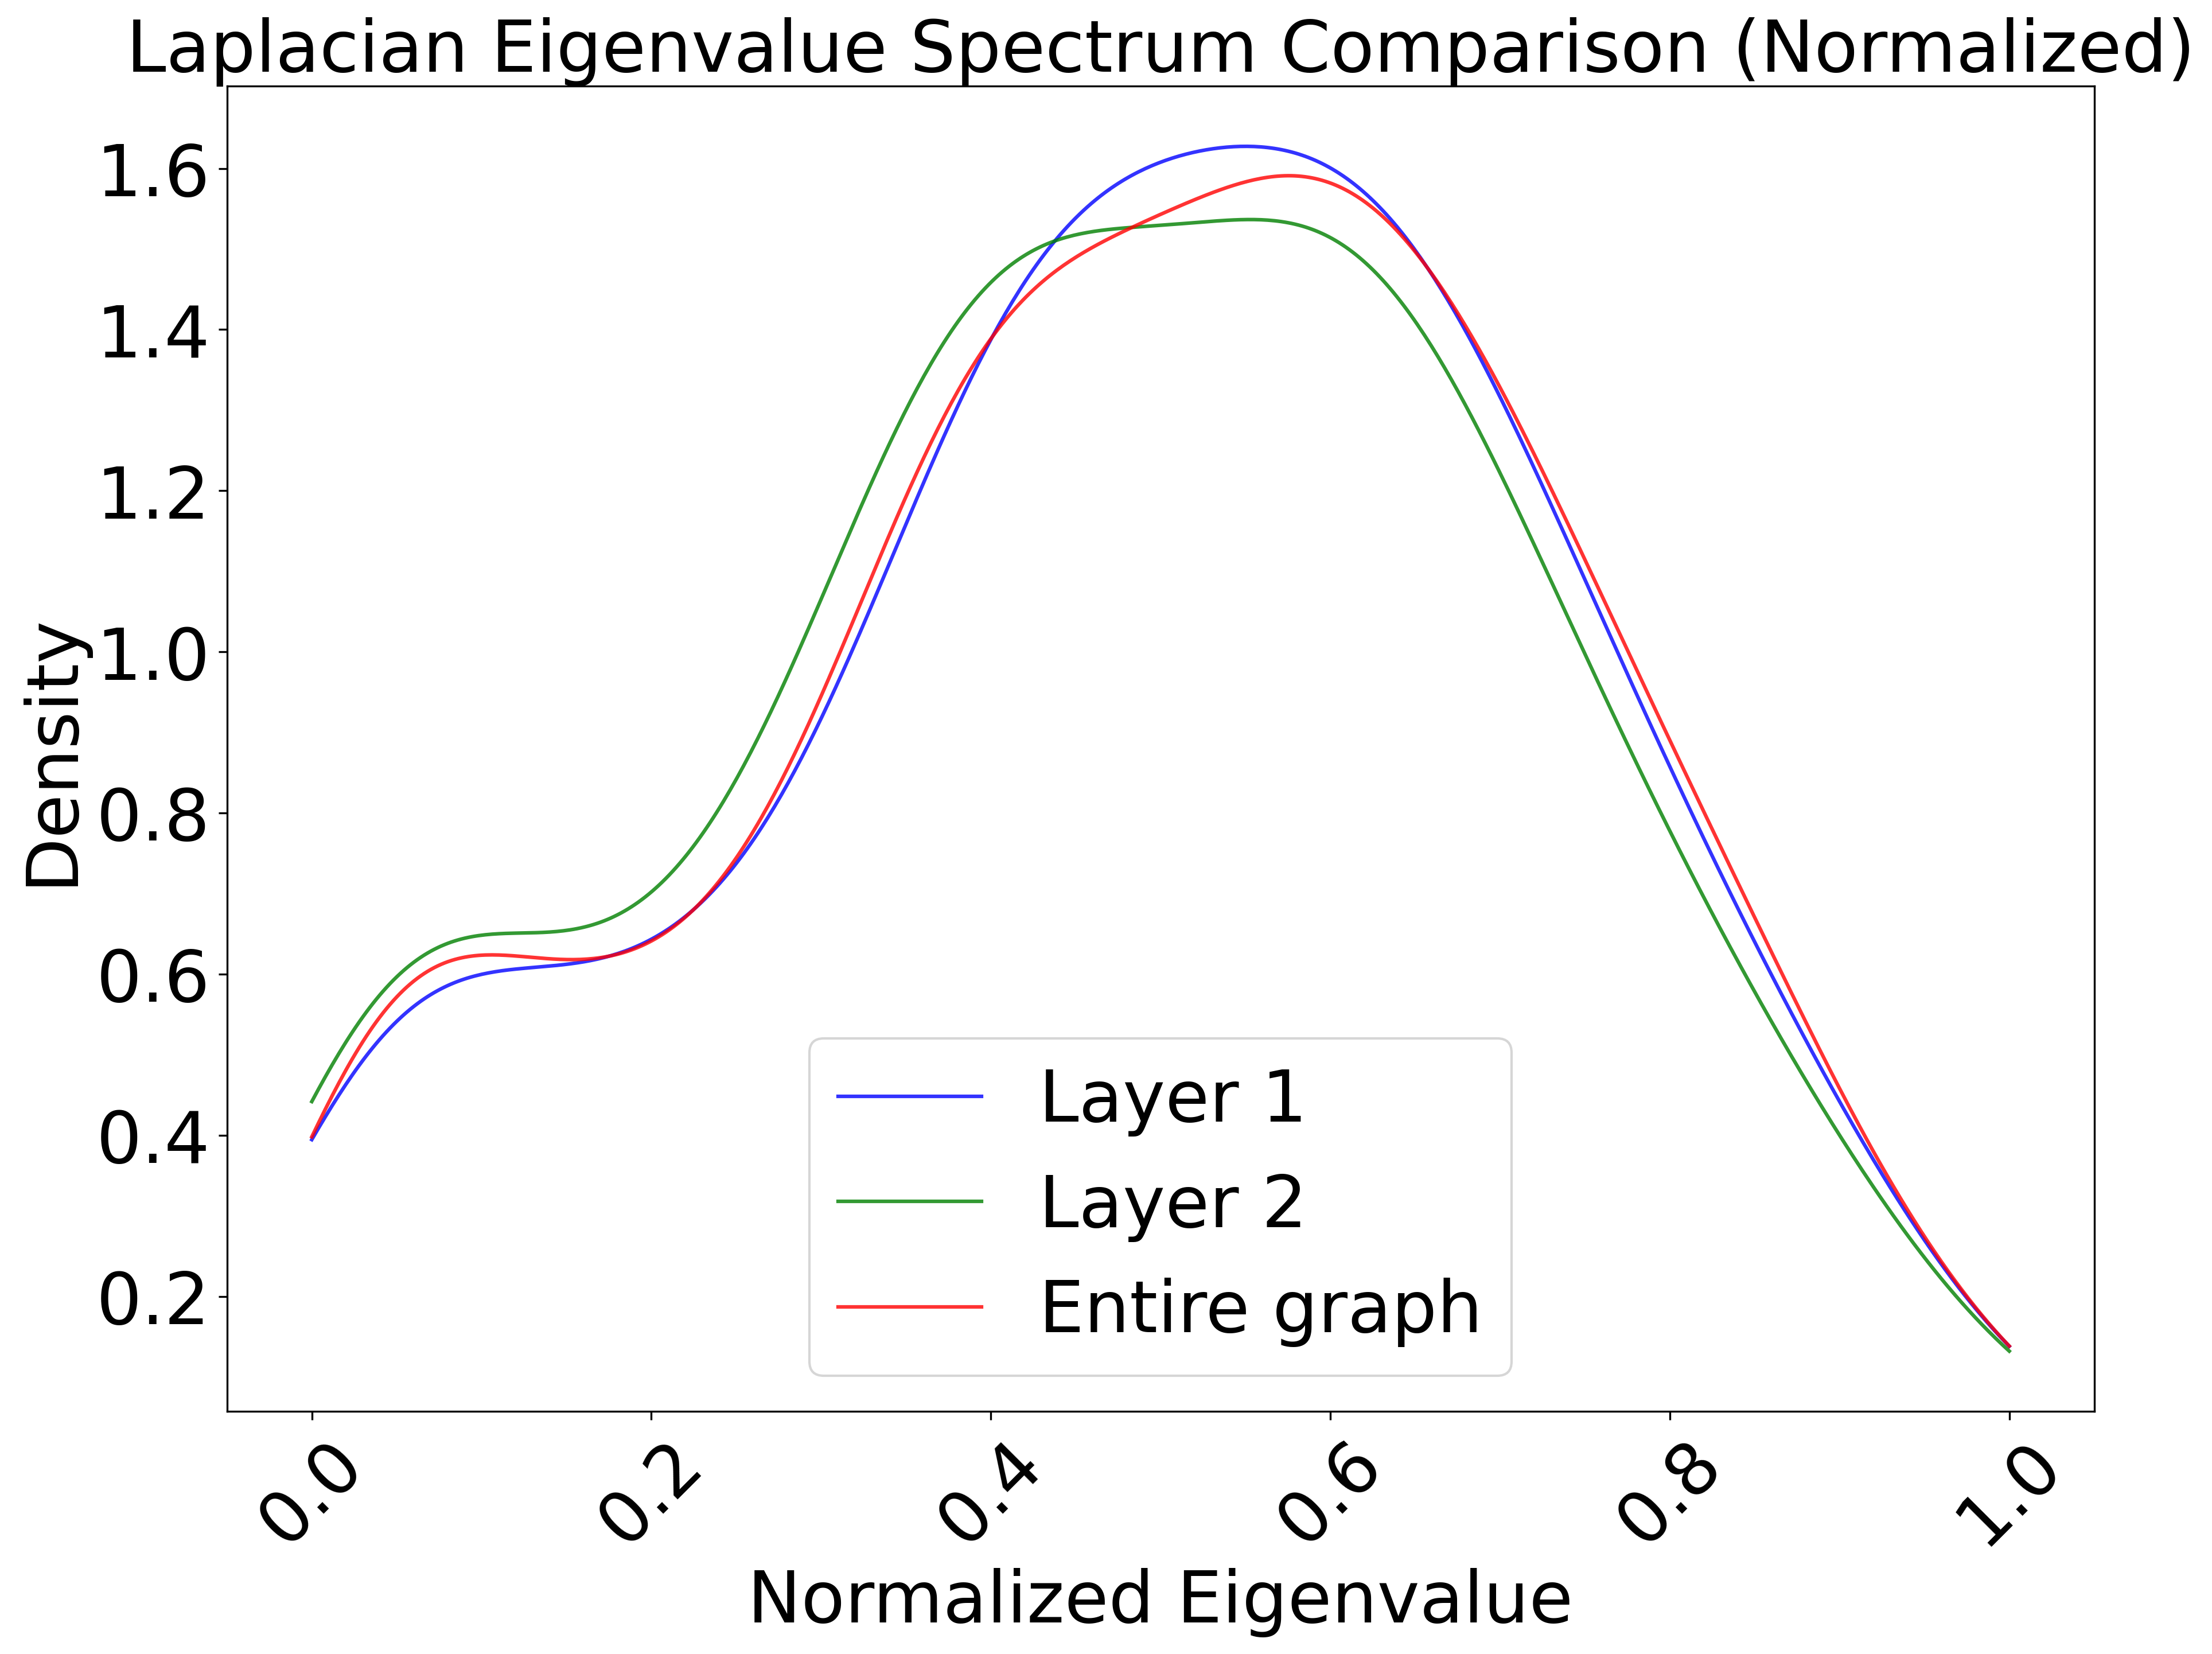
\includegraphics[width=\textwidth]{figs/fig13.png}
		\subcaption{}
	\end{minipage}
	\hspace{0.5cm}
	\begin{minipage}[b]{0.25\linewidth}
		\centering
		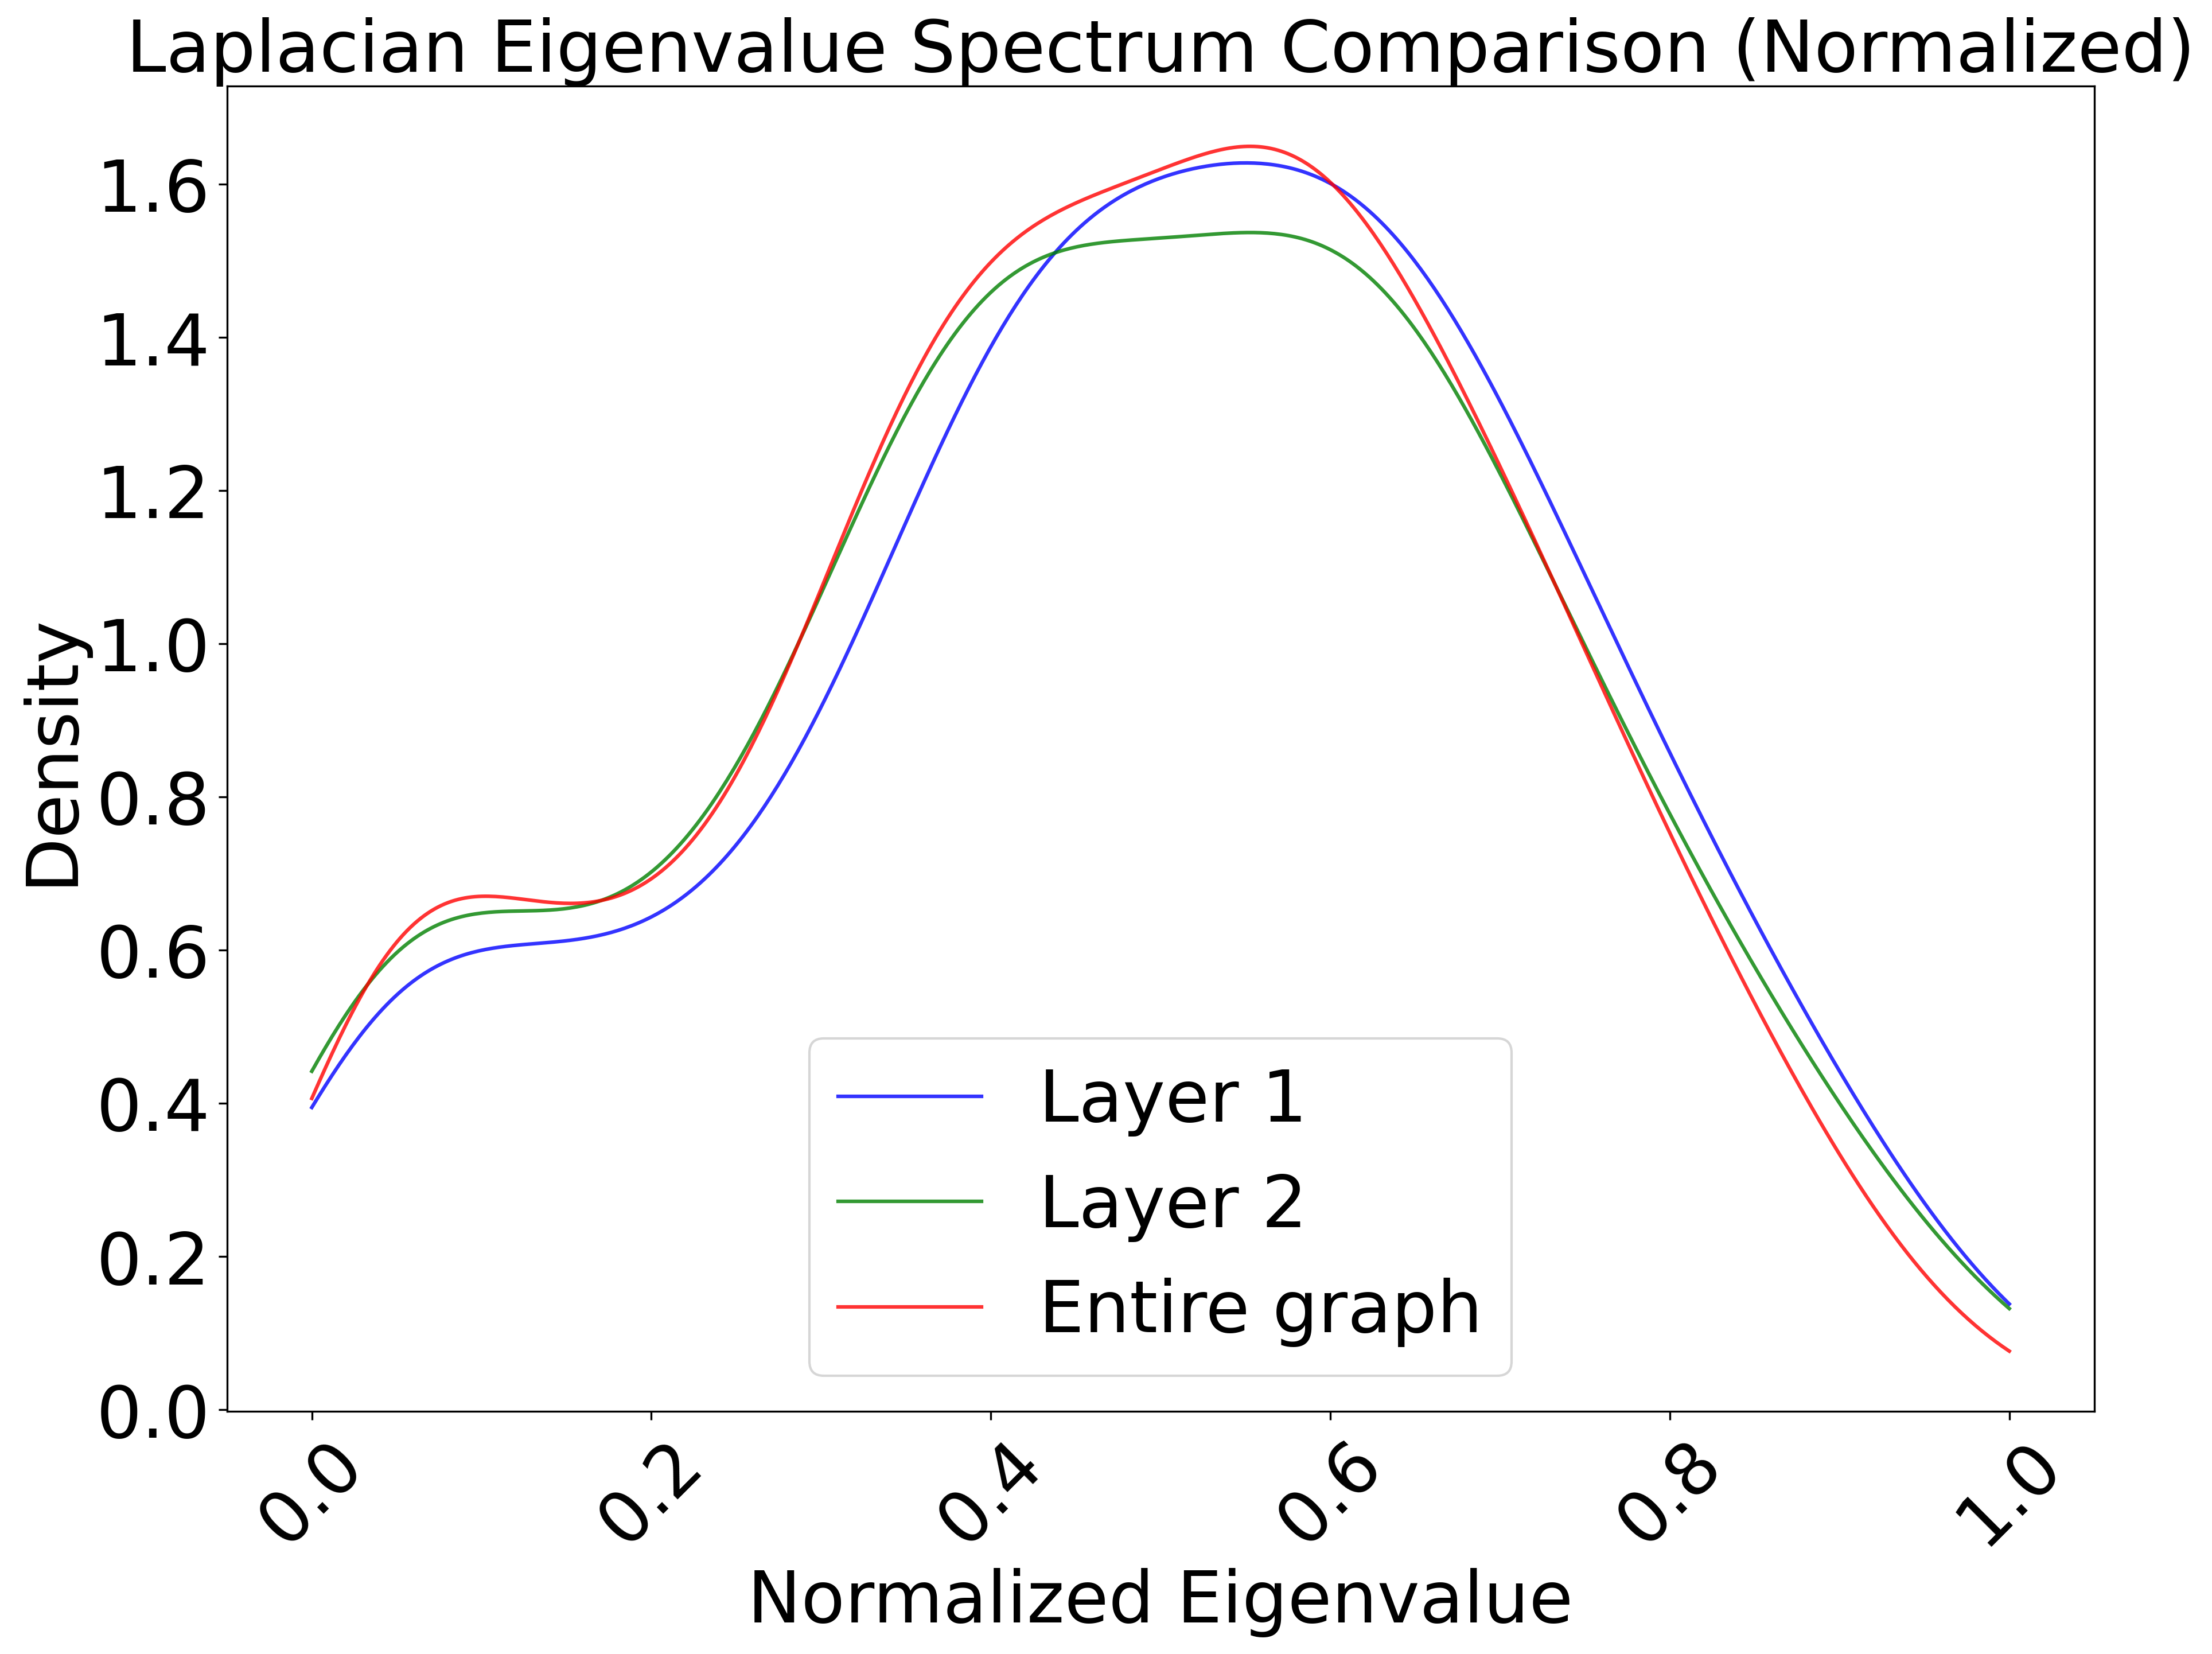
\includegraphics[width=\textwidth]{figs/fig14.png}
		\subcaption{}
	\end{minipage}
	\hspace{0.5cm}
	\begin{minipage}[b]{0.25\linewidth}
		\centering
		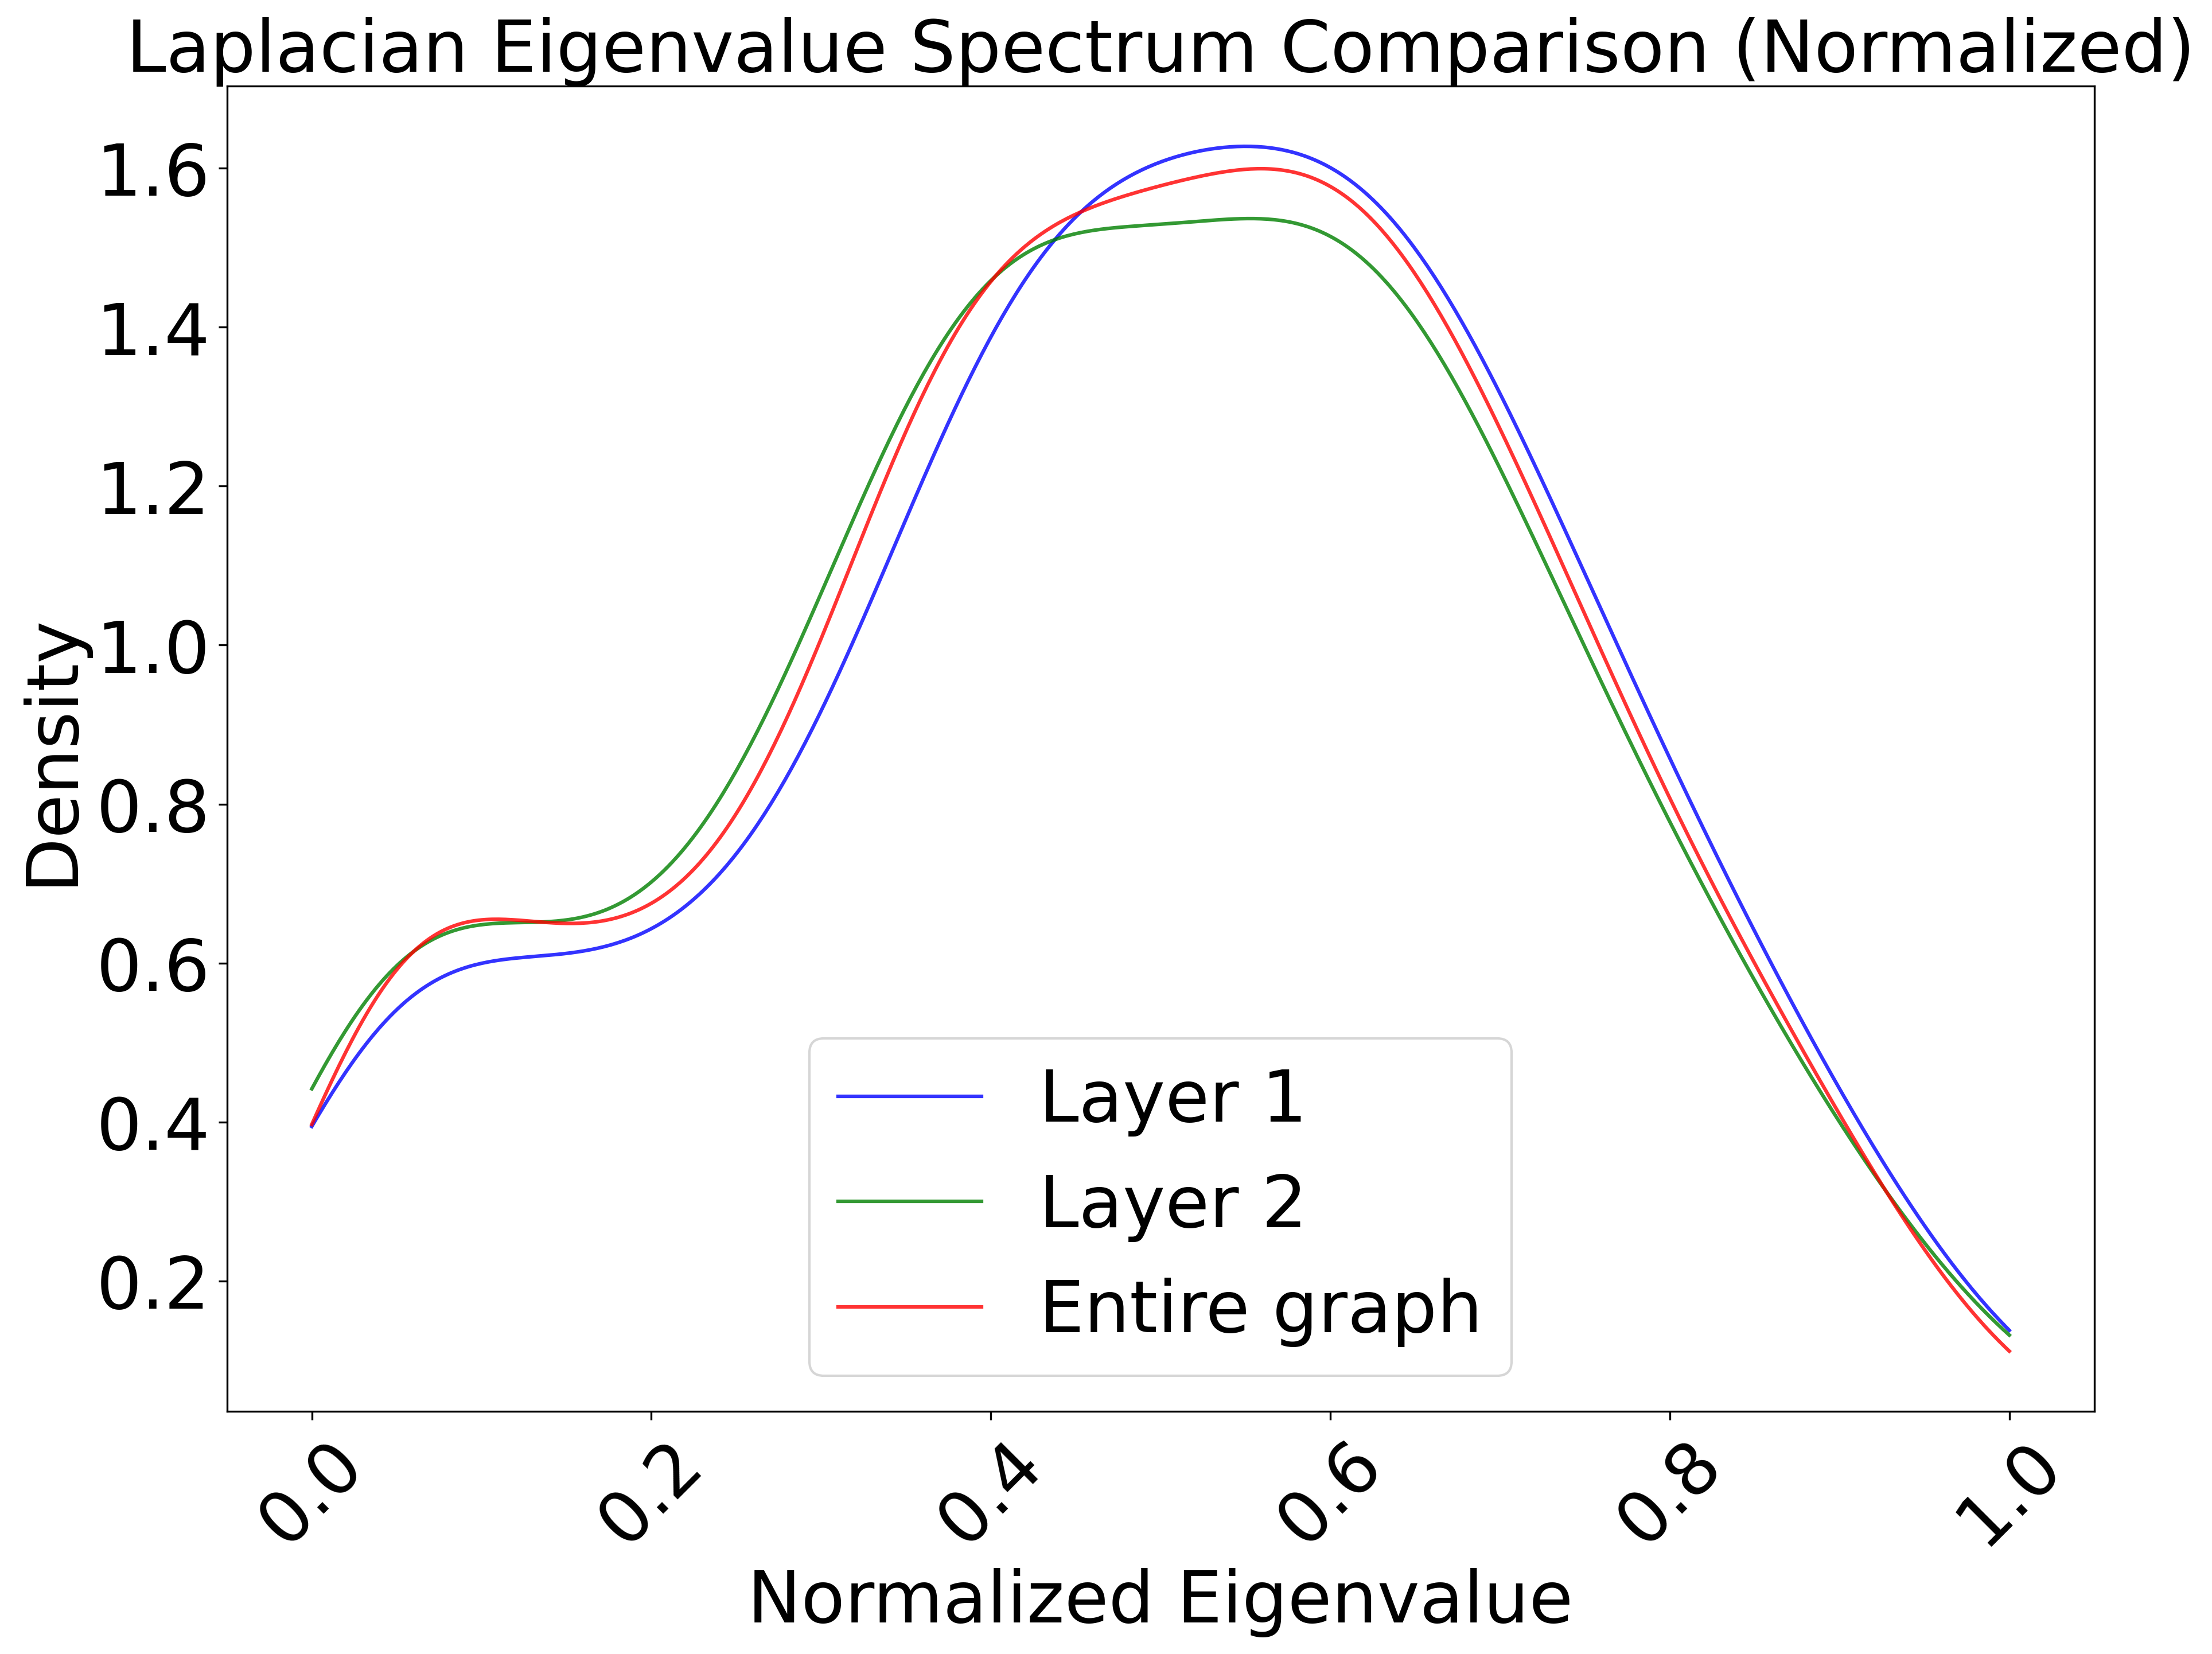
\includegraphics[width=\textwidth]{figs/fig15.png}
		\subcaption{}
	\end{minipage}
	
	\vspace{0.5cm}
	
	\begin{minipage}[b]{0.25\linewidth}
		\centering
		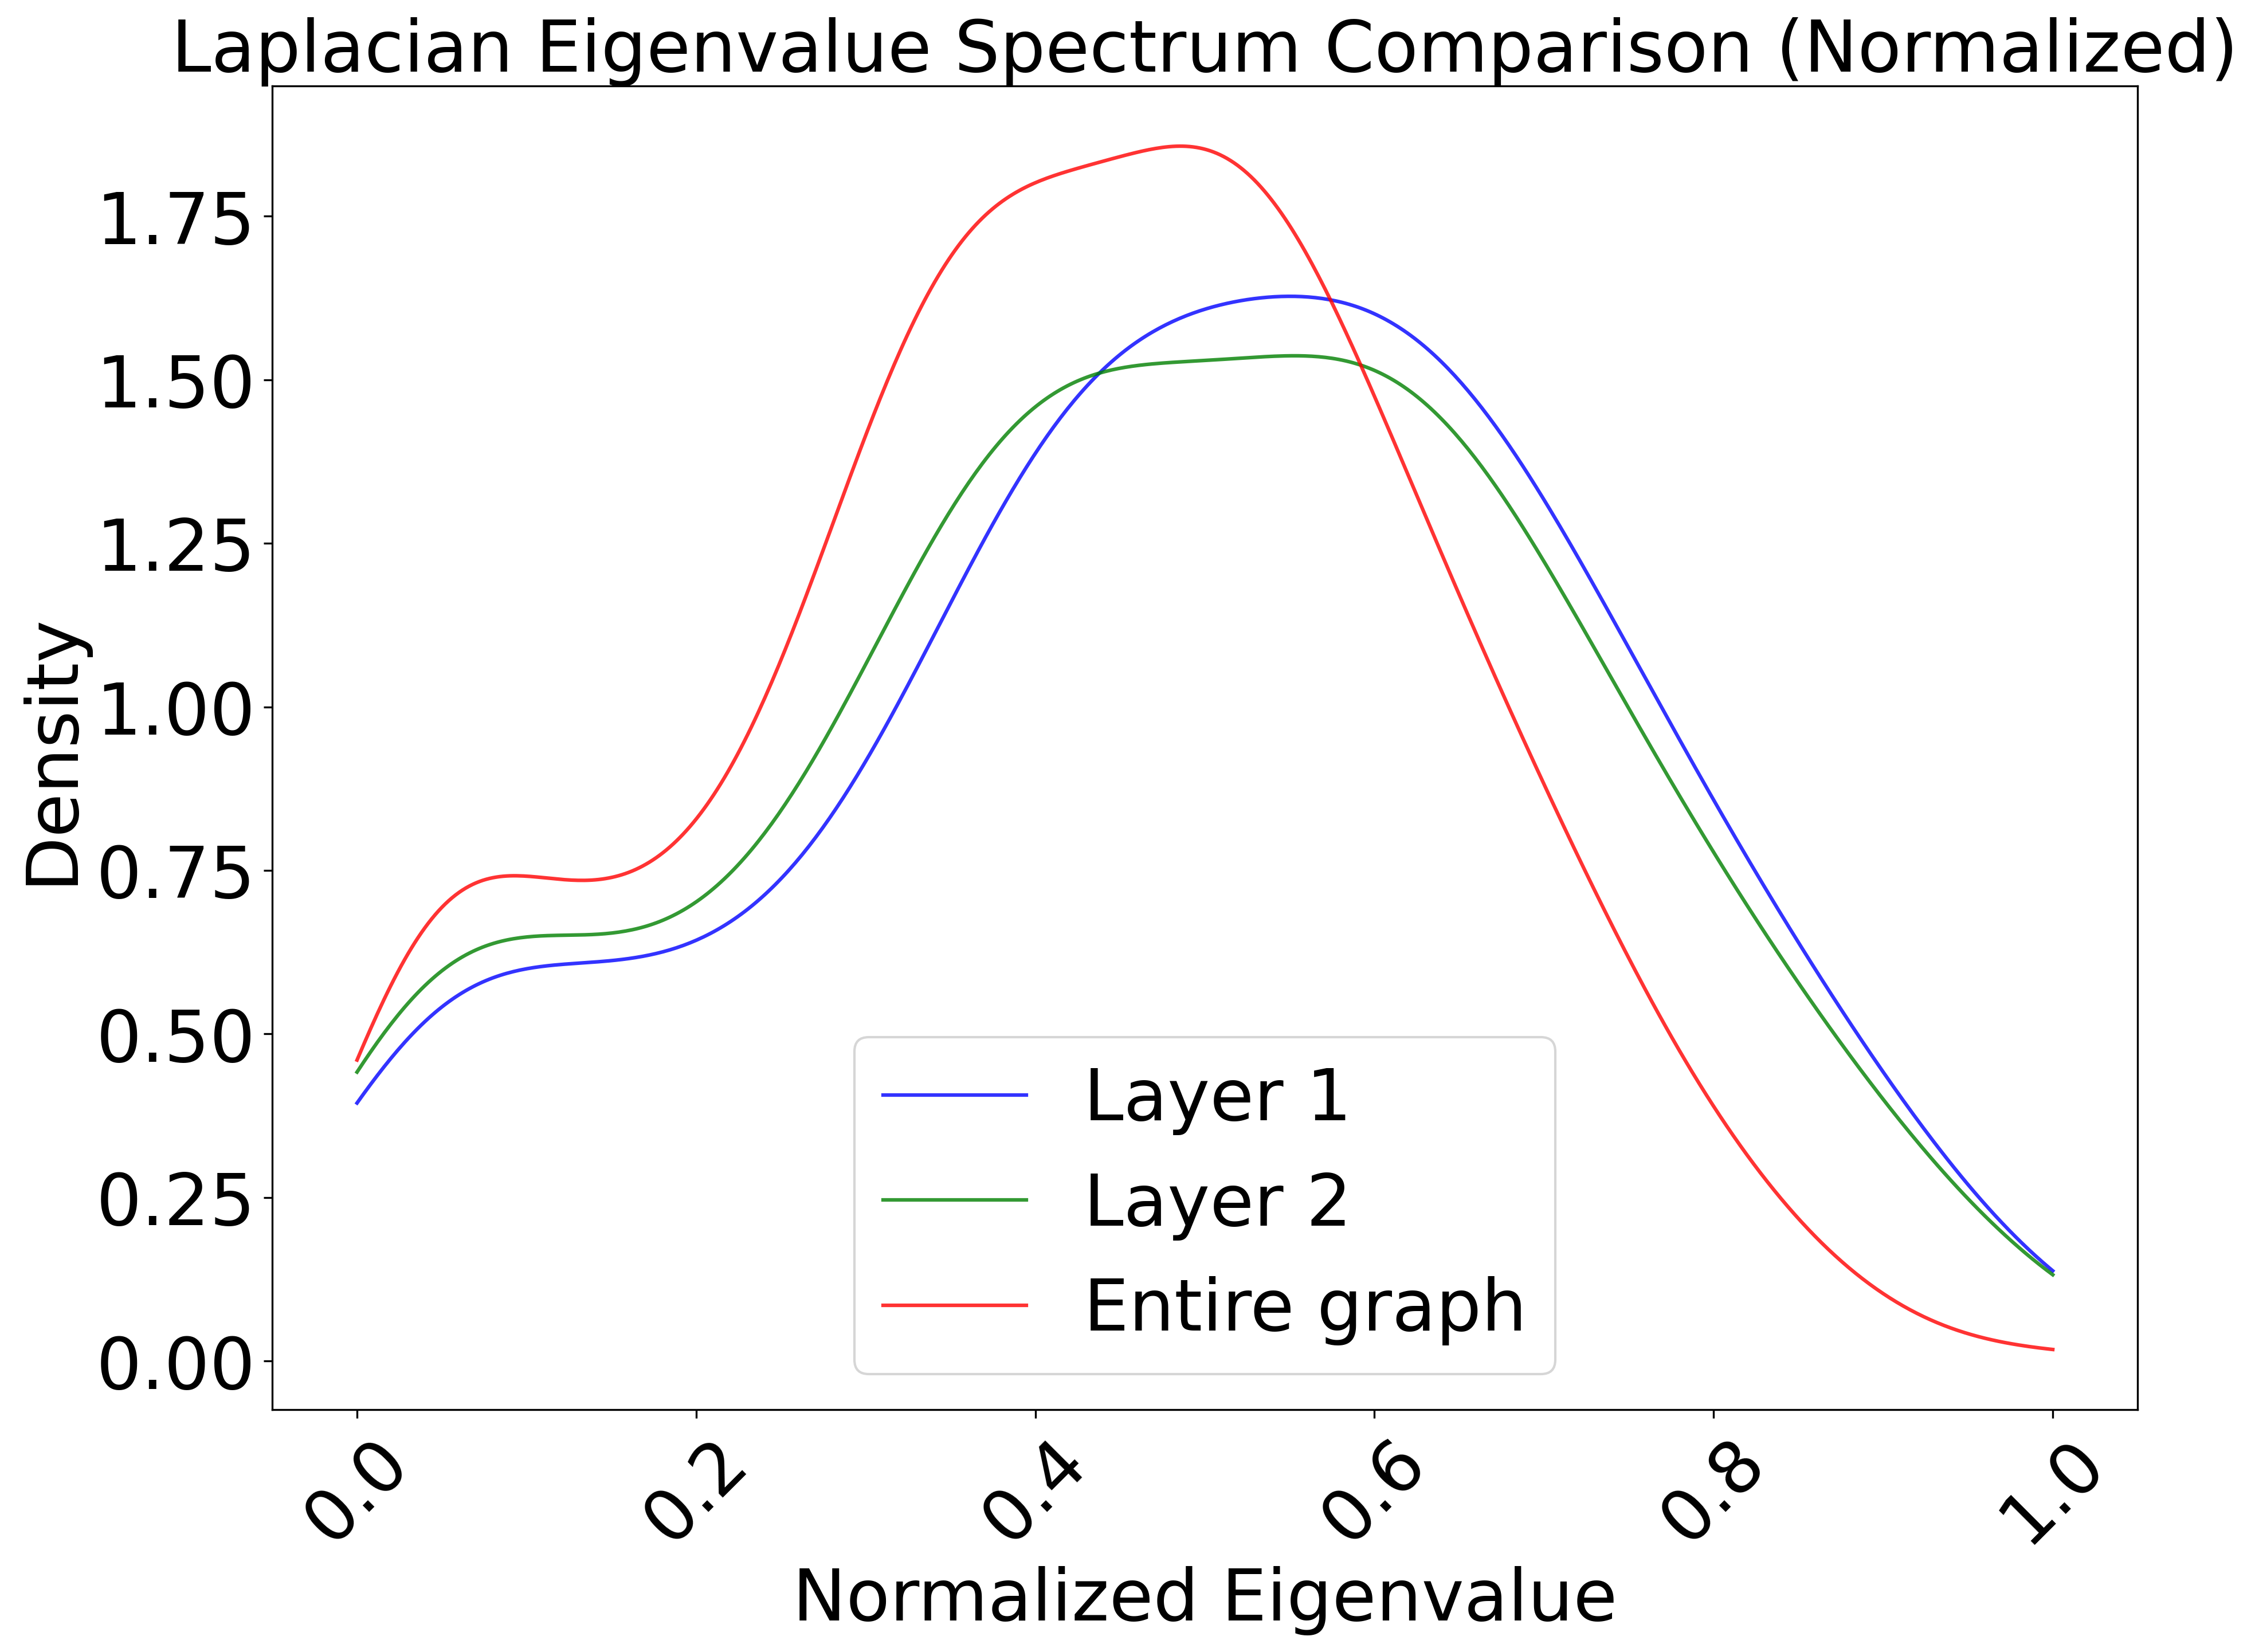
\includegraphics[width=\textwidth]{figs/fig16.png}
		\subcaption{}
	\end{minipage}
	\caption{(a) Spectral distribution of intra layer graphs and the entire graph. Spectral distribution of intra layer graphs and the entire graph using random interface configurations. (b) Random interface 1. (c) Random Interface 2. (d) Random Interface 3. \label{fig:spectral}}
\end{figure}

When single layer centrality such as Eigen vector centrality values of individual interlayer networks are compared with node modularity contribution to underlying communities (as seen in Figure~\ref{fig:modvcen} (b)), we clearly see that as the intralayer centrality and modularity values increase, there is no correlation between them. This shows that there must be some interdependence between the interlayer networks and intralayer structures. 

\subsection*{Intra versus inter layer dynamics}
Sparsity of edges in interlayer connections is strictly more than that in intralayer connections. Exploring this further, modularity of individual CLOCK and Bmal2 networks (0.71 and 0.71) is slightly less than that of the entire complex network (0.77). In addition to restrictive interlayer sparsity, this shows that inter-layer modularity depends on the intra-layer communities. From the view of multilayer formalism, let inter-layer modularity be defined as:
\begin{equation}
\label{eqn2}
Q_{inter} = \omega \sum_{i, j} A_{ij}^{Inter} \delta(c_{i},c_{j})
\end{equation}
where $\omega$ is inter-layer coupling strength and $A_{i,j}^{Inter}$ is the inter-layer connection between $i$, $j$, and as before, $\delta(c_i, c_i)$ is 1 if nodes $i$ and $j$ are in the same community and 0 otherwise. 
%Let $\gamma$ signify the resolution parameter for inter-layer modularity calculated in Equation~\ref{eqn1}. 
Quantifying the inter-layer contribution in the overall modularity based on Equation~\ref{eqn2} gives 0.41. The total modularity thus is 0.71+0.41, which is 1.12. Figure~\ref{fig:modvcen} (a) shows that inter-layer communities depend on the intra-layer structure. Figure~\ref{fig:modvcen} (h) shows the community structure of the entire protein complex graph. In Figure~\ref{fig:modvcen} (g), communities are detected for each intra-layers separately. The inter-layer connections are plotted using dashed lines. The figure (h) shows that inter-layer edges connect to similar communities between layers. 

Figure~\ref{fig:modvcen} (c) shows that Multicens captures inter layer modularity better than eigen-vector centrality. Not all inter layer edges contribute to overall modularity directly as the intra layer structures influence inter layer connections. Multicens, by modeling inter layer transitions based on intra layer rankings, models hierarchical relationship between inter and intra layer edges. It distinguishes modularity of intra and inter layer nodes between than eigen vector centrality. Eigen vector centrality has low values for most intra layer nodes and lacks the granulairty of information capturing dependence between intra and inter layer modularity. Intra and inter layer centrality of multicens are better correlated with multi-layer modularity than that of eigen vector centrality. In the case of eigen vector centrality, most of the nodes have low centrality regardless of their modularity (or contribution to community formation). 

Figures~\ref{fig:modvcen} (d), (e), and (f) show intra and inter layer centrality vs modularity for random inter layer configurations. On the left, inter layer configuration is random. As we move to the right, the topology of the interface gets closer to the original. Relationship between Inter/Intra layer modularity captured by Multicens helps it distinguish random inter layers better than eigen vector centrality. In Multicens, intra layer modularity changes across different random interlayers, whereas in eigen vector centrality, intra layer modularity does not change much across different random inter layer configurations. Furthermore, Multicens places emphasis on the inter layer structures and thus intra layer patterns change across the various random inter layer configuration even though intra layer structures remain unchanged. 

Multicens captures relationship between strong ties and bridges better than eigen vector centrality. A strong tie is an edge whose vertices belong to the same community. A bridge is an edge whose vertices belong to different communities. No strong tie is a bridge; some inter layer edges are strong ties and rest are bridges. By modeling interdepence between intralyer and interlayer structures, Multicens distinguishes strong ties and bridges (as shown in Figure~\ref{fig:ties1} (a)) by scoring bridges in a broader range (i.e. strong ties are central while bridges may or may not be) than strong ties' centrality values. 


Figures~\ref{fig:ties1} (b),~\ref{fig:ties2} (a), (b) show that Multicens has clear grouping patterns for different random inter layers for bridges and strong Ties; eigen vector centrality does not (indicating existence of dependence between intra/inter layer structures). On the other hand, eigen vector centrality captures spectral properties that model local and global properties of the graph structure. Spectral distribution (as shown in Figure~\ref{fig:spectral} (a) for original interface and Figures~\ref{fig:spectral} (b), (c), (d) for random interlayer configurations) clearly distinguishes random from original interfaces. Local and global structural properties captured by the spectral distribution ensures that the overall network's distribution must lie within those of the individual intra layer networks. Thus, a random interface that is topologically similar to the original interface is detected to modify global structure of the network. 

Thus, the hypothesis is that devising a centrality measure that captures both: (a) modularity as a factor of the interdependence of interlayer configuration on intralayer structures, and, (b) properties capturing local and global properties together, can help understand the interlayer and intralayer node properties better in protein complexes. 

\section*{Multilayer Graph Centrality}
% Let sparsity of a layer be $S_{layer} = 1 - \frac{|E_{layer}|}{E_{max,layer}}$ where $|E_{layer}|$ is the number of existing edges and $|E_{max,layer}|$ is the maximum possible edges. Sparsity for Clock is $\sim$

Centrality measures such as degree, betweenness~\cite{newman12012networks}, and closeness centrality~\cite{newman12012networks} are based on static, single-layer networks. However, in complex systems such as protein complexes, connectivity is often multilayered. 
Here, we introduce a new node scoring metric derived from k-hop Jaccard similarity and matrix factorization. The goal of this metric is to quantify node importance by leveraging localized graph overlap patterns while incorporating a learned latent structure.
The metric integrates multilayered structural information using k-hop Jaccard similarity across different layers, followed by a matrix factorization approach to refine the node importance score.

\subsection*{Methodology}
For a protein complex network composed of two chains or layers, $G_{l1}$ and $G_{l2}$ (for simplicity, we consider complexes of two chains, however, the formulation can easily be extended to model complexes with many chains), and the entire graph $G$, we compute the $k$-hop Jaccard similarity for every pair of nodes $A$ and $B$ separately for each layer ($L_1$ and $L_2$) and for the entire graph:
\[
J(A,B) = \frac{|N_k(A) \cap N_k(B)|}{|N_k(A) \cup N_k(B)|}
\]
where $N_k(A)$ represents the $k$-hop neighborhood of node $A$ and $N_k(B)$ represents the $k$-hop neighborhoood of node $B$. The $k$-hop Jaccard similarity matrix captures local node connectivity by measuring the fraction of shared neighbors within a $k$-hop neighborhood.
The self-similarity matrices for $l1$ and $l2$ are scaled and placed into respective blocks of a larger matrix $W$, capturing intra-layer relationships.
We construct the following overlap matrices:
\[W = 
\begin{bmatrix}
scale(W_{L1}) & 0 \\
0 & scale(W_{L2})
\end{bmatrix}
\]
where $W_{L1}$ is similarity matrix for Layer 1, $W_{L2}$ is similarity matrix for Layer 2, and scaling ensures comparable magnitudes across layers. 

An initial random matrix $A$ is generated, which serves as the latent structure to be learned. 
The optimization objective minimizes the difference between $WA$ and $X$, incorporating an $L_2$-regularization term:
\[
min_A ||WA-X||^{2}_{F} + \lambda||A||^{2}_{F}.
\]
To refine node scores, we perform an iterative learning process using gradient-based optimization~\cite{ruder2016graddes}:
\[
A^{(t+1)} = A^{(t)} - \eta[2W^T (WA - X) + 2\lambda A]
\]
where $\eta$ is the learning rate, $\lambda$ is a regularization term, $A$ is the learned weight matrix, randomly initialized, and $X$ is the similarity matrix for the entire network ($G$). 
Finally, the multilayer centrality (MLC) score for each node is obtained by summing the row-wise product of $W$ and $A$:
\[
Node Score = \sum (WA)_{row}.
\]
This approach integrates local and global structural properties while leveraging the multilayer structure. This effectively learns a transformation matrix that aligns local structures (as captured by $W$) with global node relationships (encoded in $X$).
This aggregation captures how much each node contributes to the learned latent structure, effectively ranking nodes based on their structural significance in the graph.

Unlike degree centrality, which considers only local edges, our metric integrates layer-wise connectivity and global network structure. The use of $k$-hop Jaccard similarity ensures that node importance reflects not just immediate neighbors but also higher-order neighborhood overlap. Instead of treating all edges equally, the matrix factorization learns node importance, improving robustness over static measures. 

\subsection*{Multicens~\cite{kumar2023multicens}}
Multicens addresses the challenge of modeling interlayer influence in complex networks by separating intralayer influence of nodes with their interlayer influences. Local centrality isolates a node’s influence within its layer using a modified PageRank algorithm applied to intralayer adjacency matrices ($A[i]$s). By nullifying interlayer connections, it identifies nodes that coordinate localized influences for a particular layer, $i$. The iterative equation:
\[
l_{layer_{i}}^{(k+1)}=pA^{[i]}l_{layer_{i}}^{(k)}+\frac{(1-p)}{n}1^{i}
\]
prioritizes the node influence within each layer. Here, $l_{layer_{i}}^{(k)}$ represents layer $i$'th node scores in iteration $k$, $1^{i}$ is a vector with entries for nodes in layer $i$ set to 1 and 0 otherwise, $n$ is the number of nodes, and $1-p$ being the probability that a random walk restarts from any node in the network. 

The global centrality captures the remaining effect of a random walk continuing to any node regardless of layer and is given by:
\[
g^{(k+1)}=p[(A+C)g^{k} + Cl]+\frac{(1-p)}{N}1
\]
Here $g^{k}$ represents the overall node scores in iteration $k$, $1$, as previously, is a vector with entries for nodes in the network set to 1 and 0 otherwise, $N$ is the total number of nodes in the network, and $p$ being the probability that the random walk continues either within the same layer or jumps to another layer, $A$ represents the adjacency matrix with intralayer connections, and $C$ represents the adjacency matrix with interlayer connections. 

%~\cite{bailey1977theory,wang2011epidemics,feng2009networks}

\begin{figure}[h!]
\centering
\begin{minipage}[b]{0.25\linewidth}
\centering
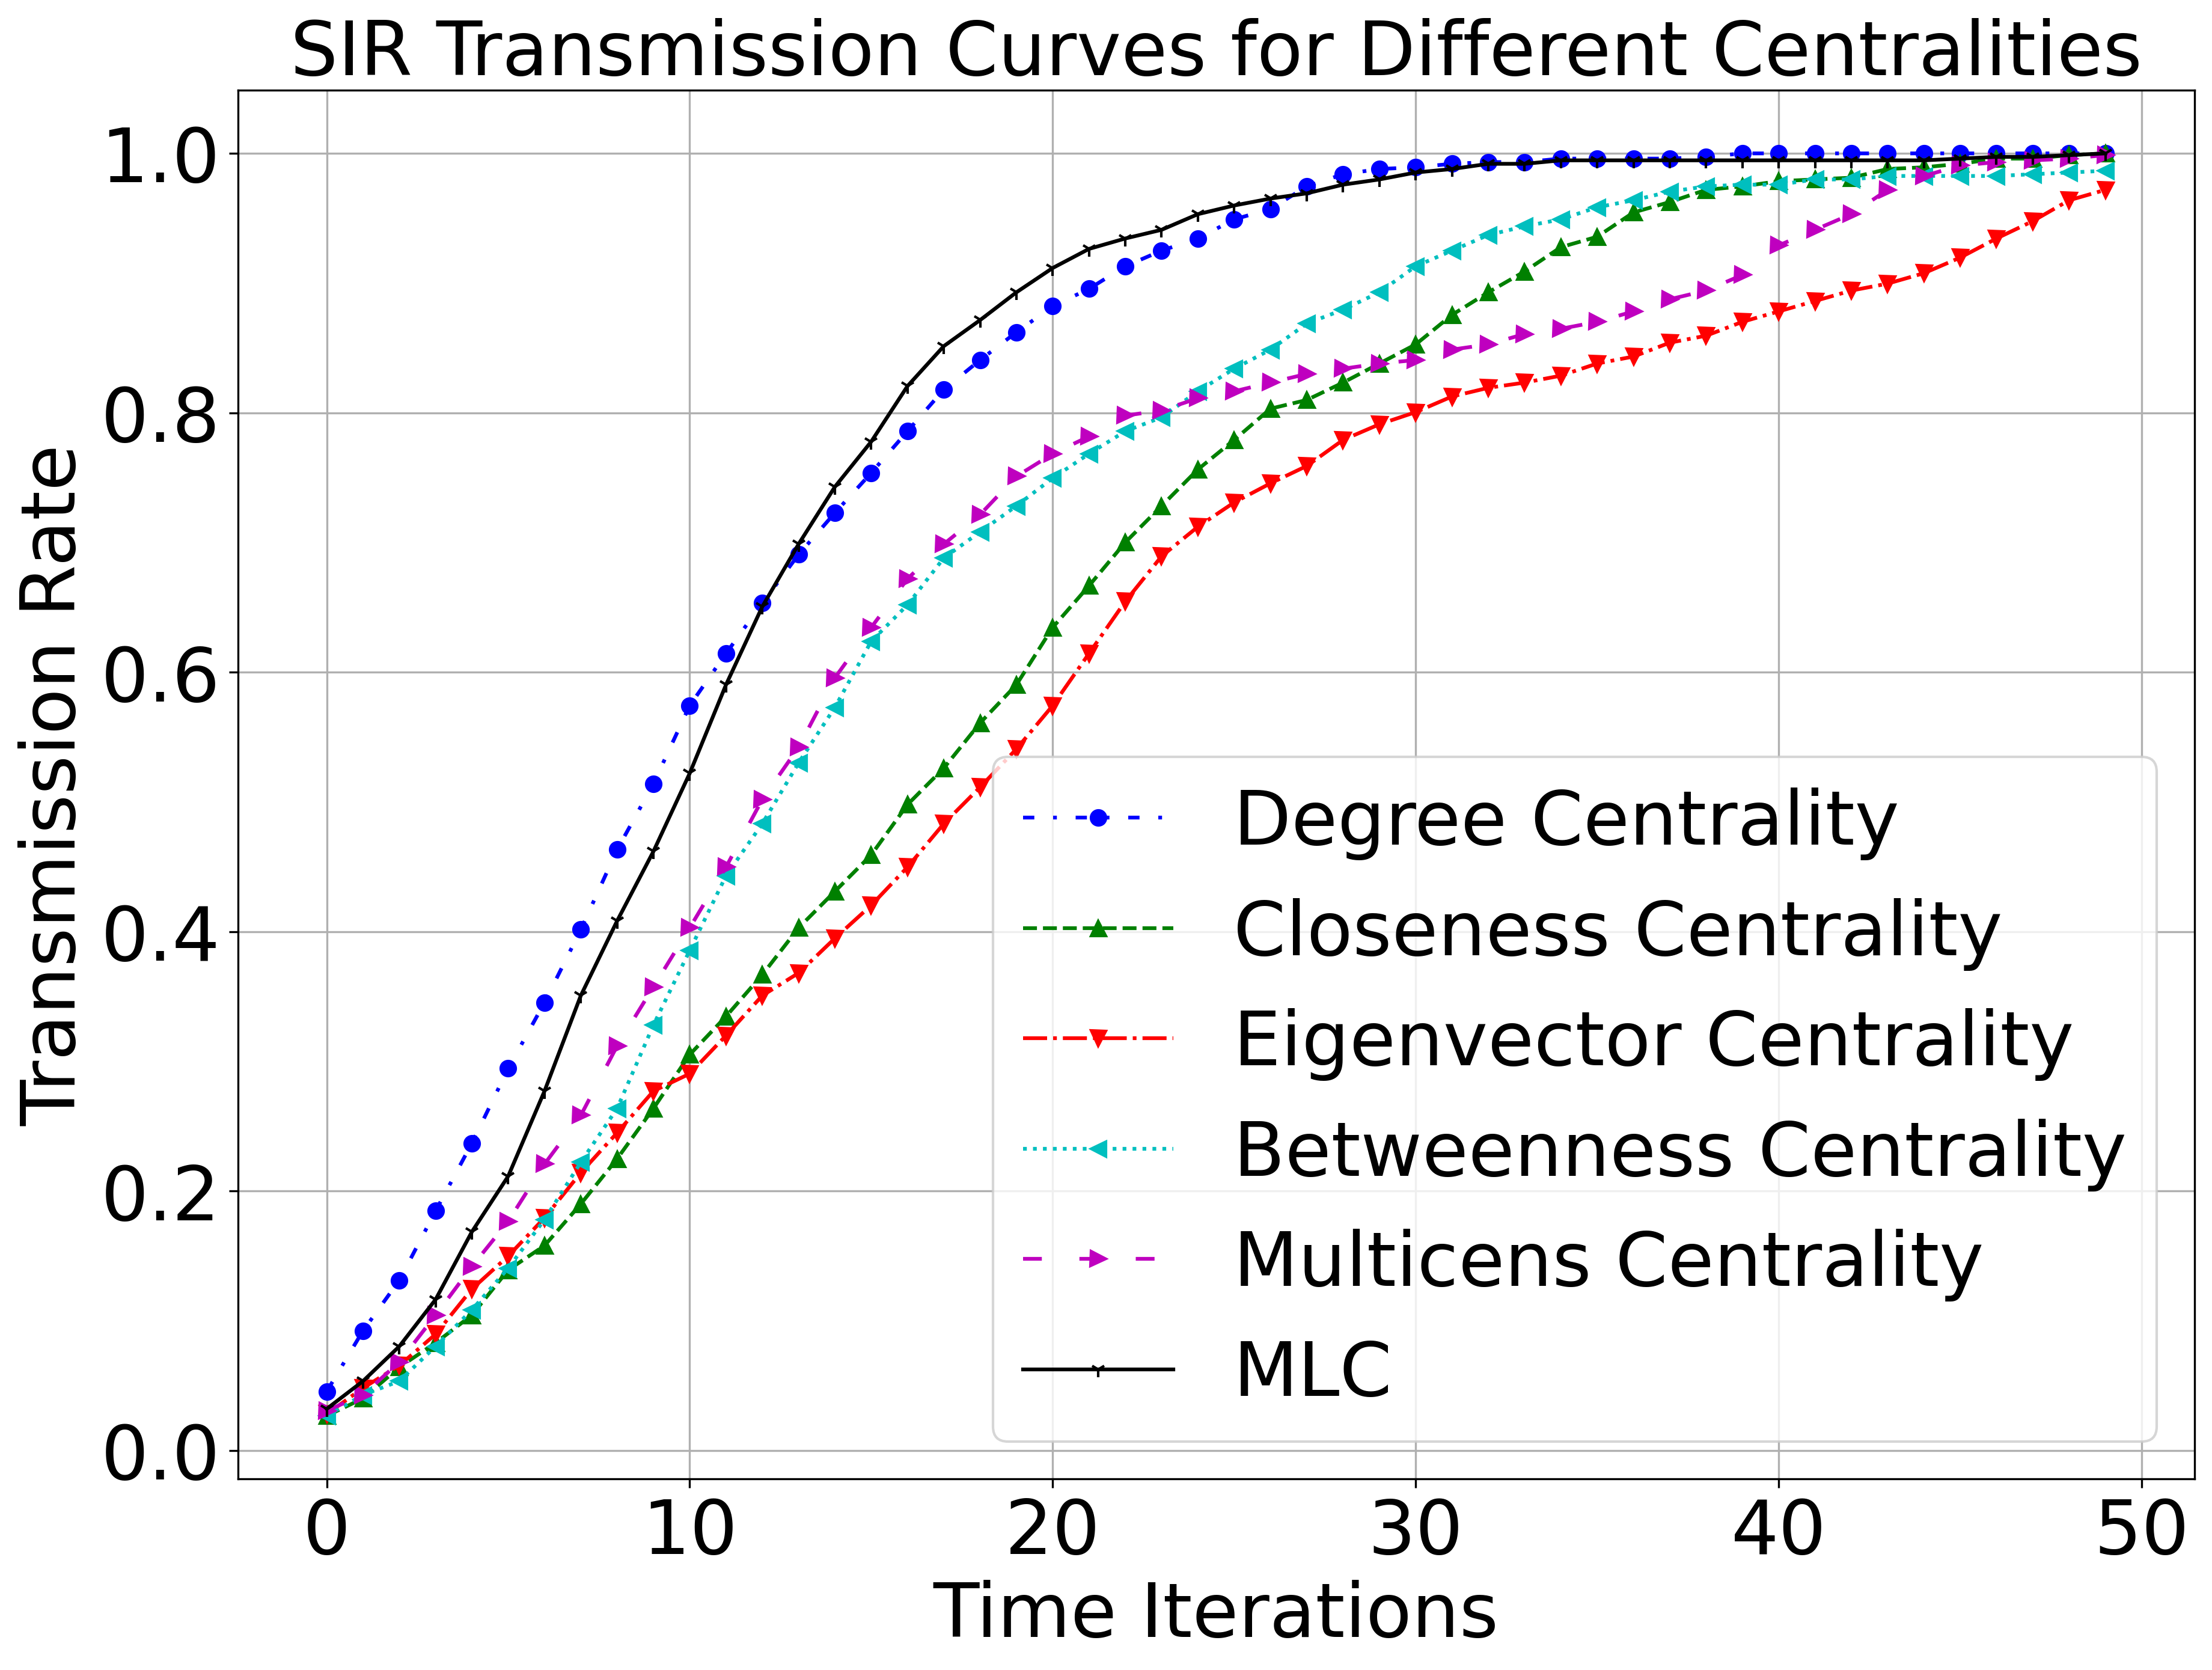
\includegraphics[width=\textwidth]{figs/fig17-ahr_arnt-k1top2.png}
\subcaption{}
\end{minipage}
\hspace{0.5cm}
\begin{minipage}[b]{0.25\linewidth}
\centering
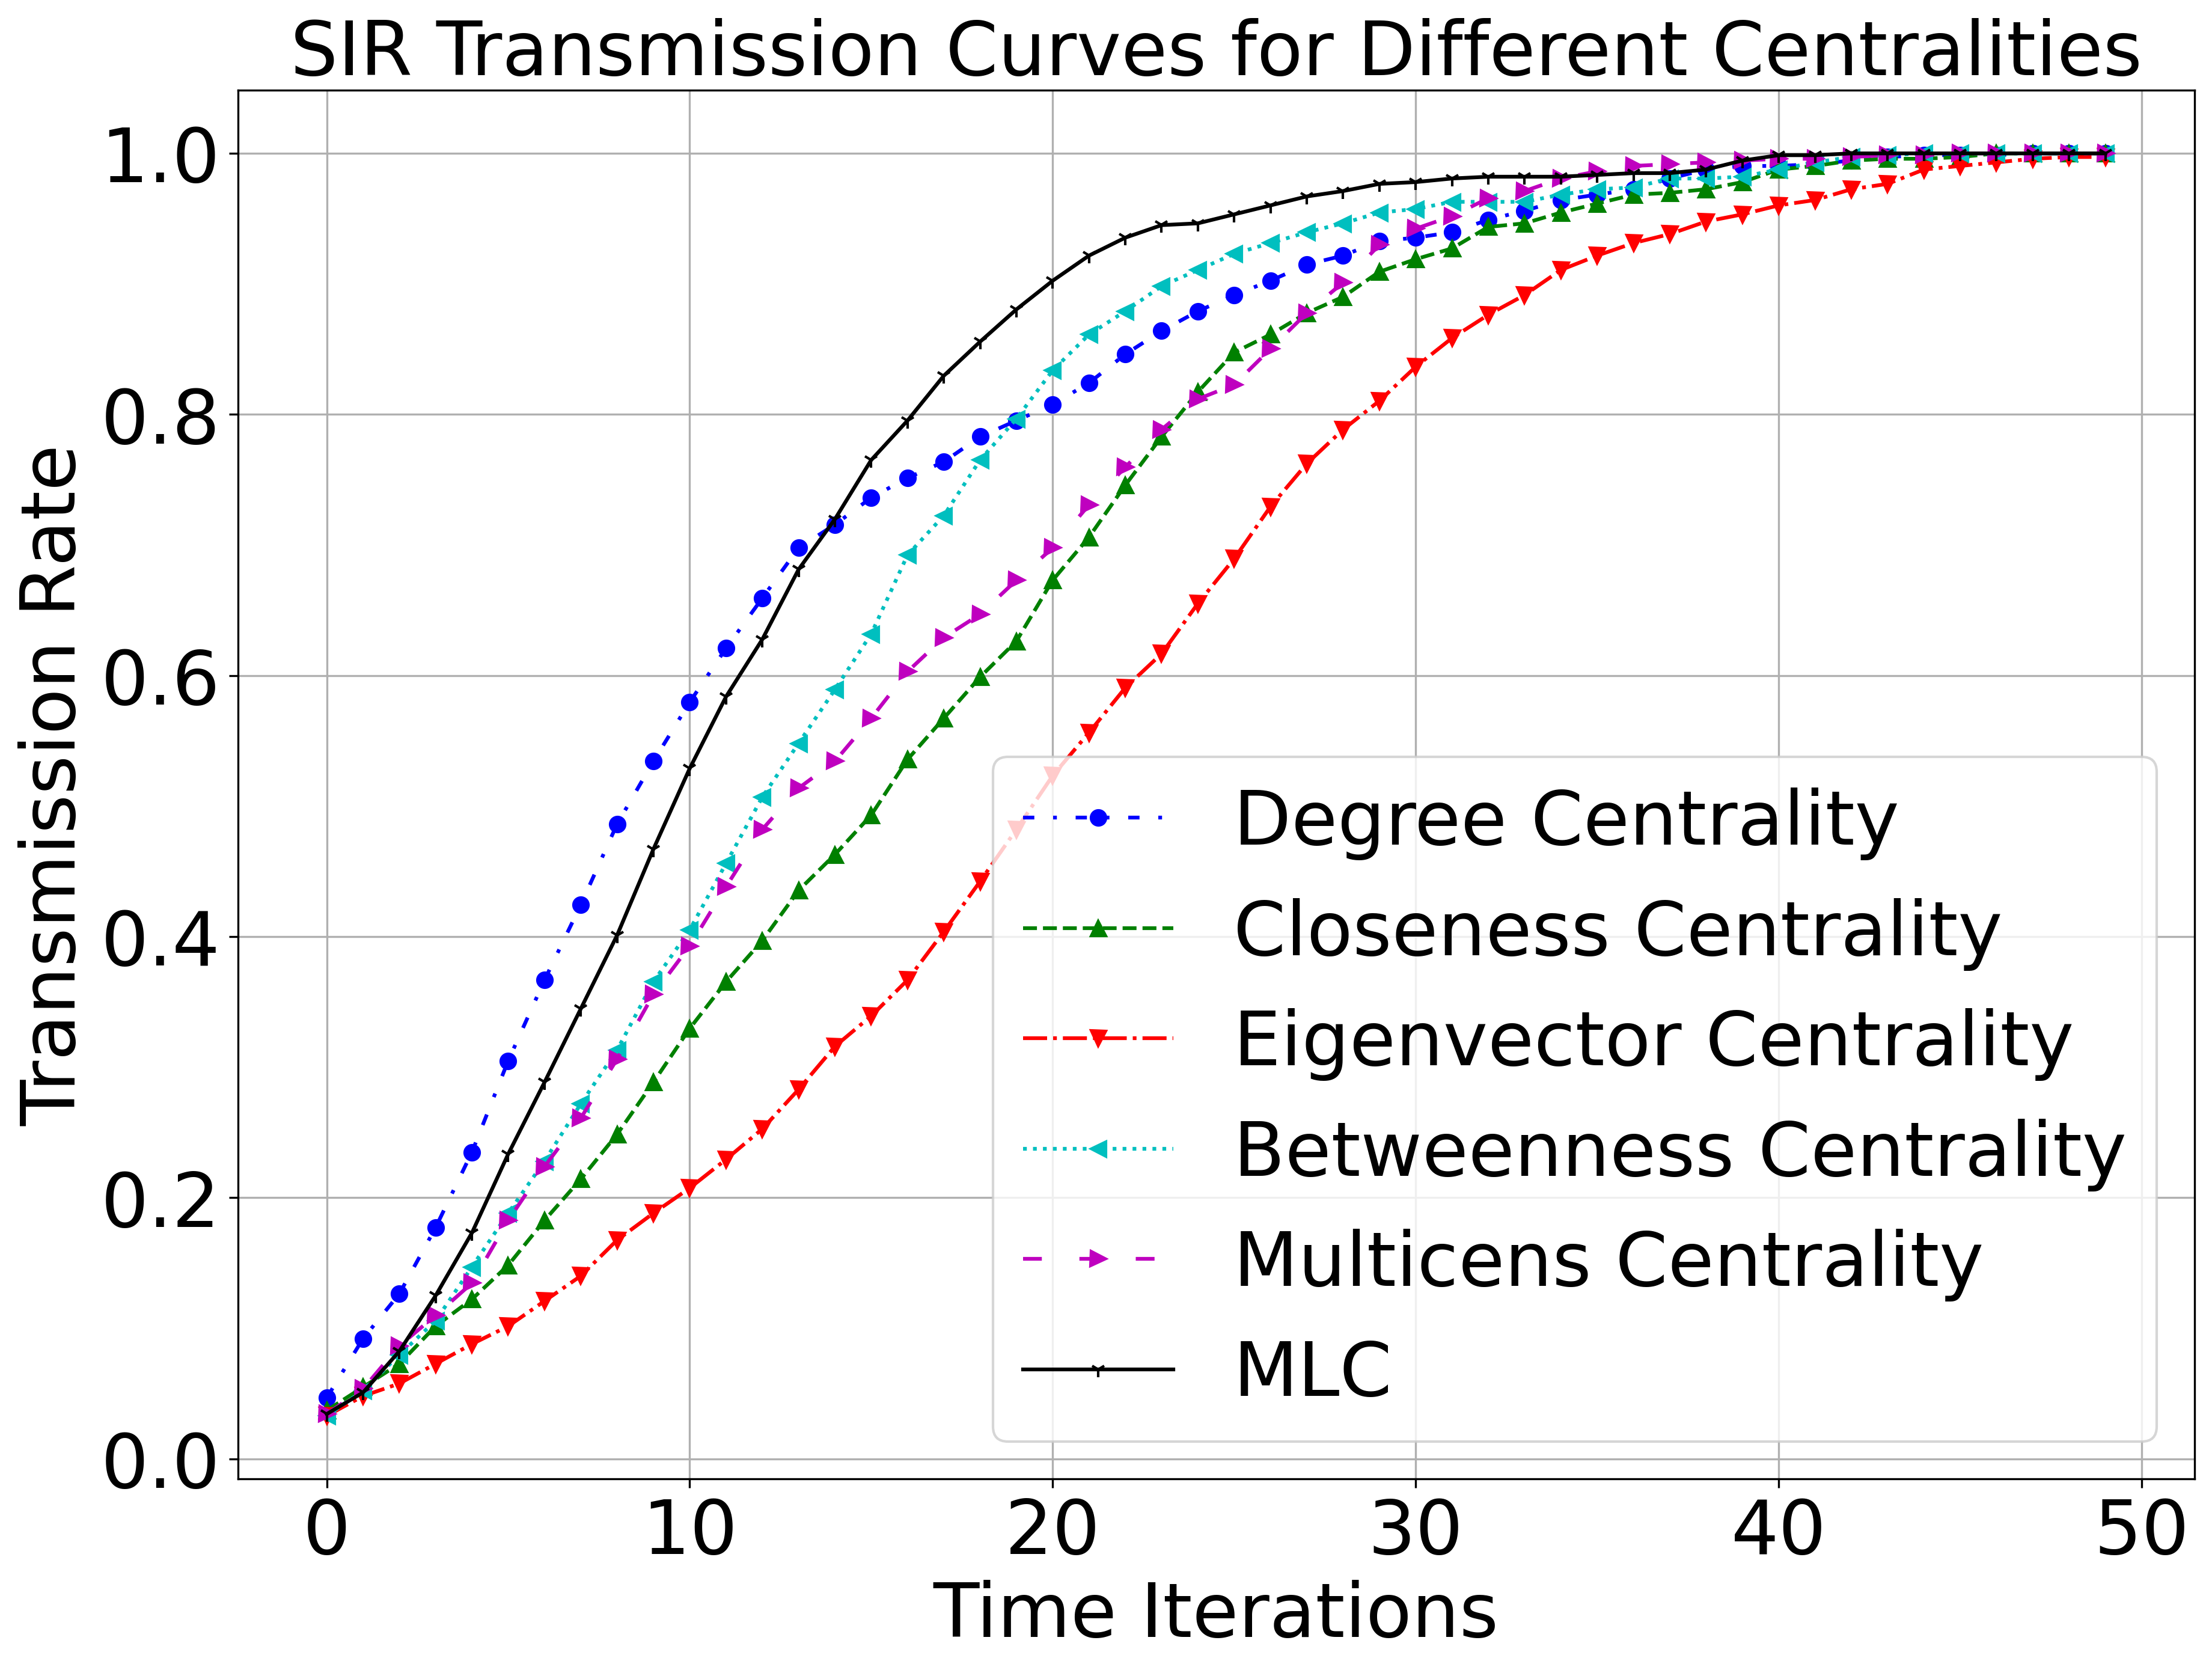
\includegraphics[width=\textwidth]{figs/fig18-clock_bmal1-k2top2.png}
\subcaption{}
\end{minipage}
\hspace{0.5cm}
\begin{minipage}[b]{0.25\linewidth}
\centering
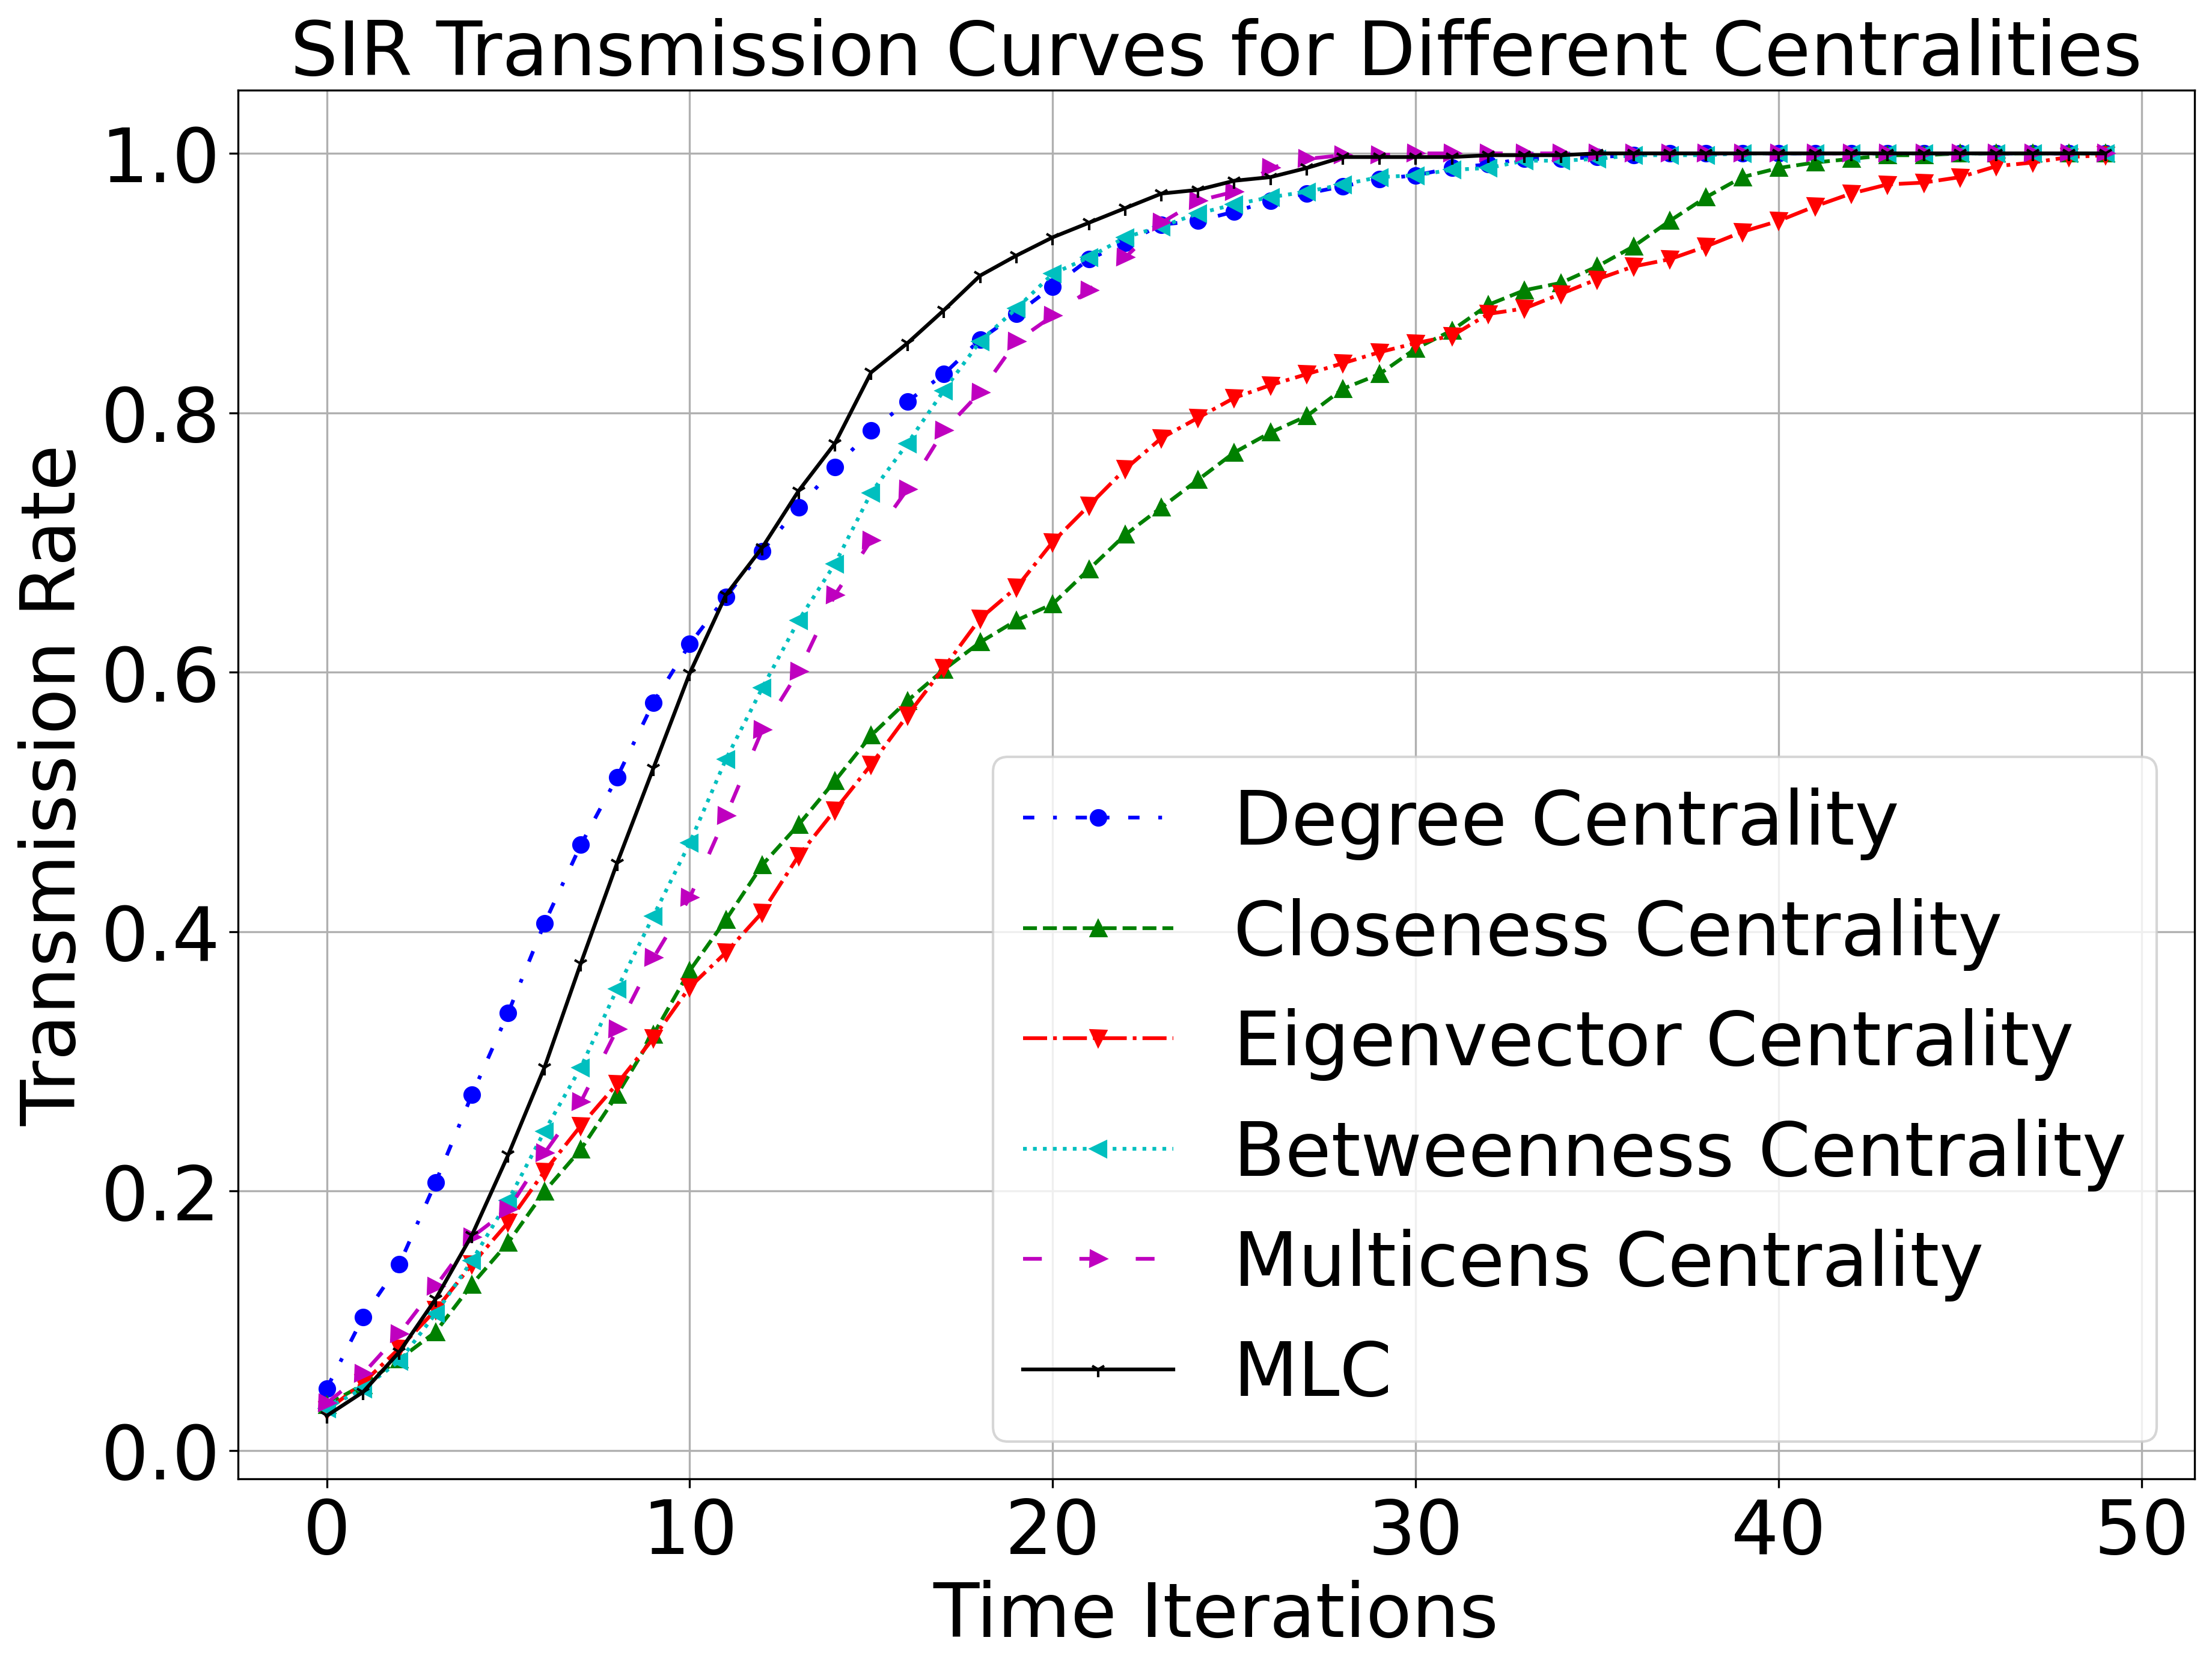
\includegraphics[width=\textwidth]{figs/fig19-hif1a_arnt-k2top2.png}
\subcaption{}
\end{minipage}

\vspace{0.5cm}

\begin{minipage}[b]{0.25\linewidth}
	\centering
	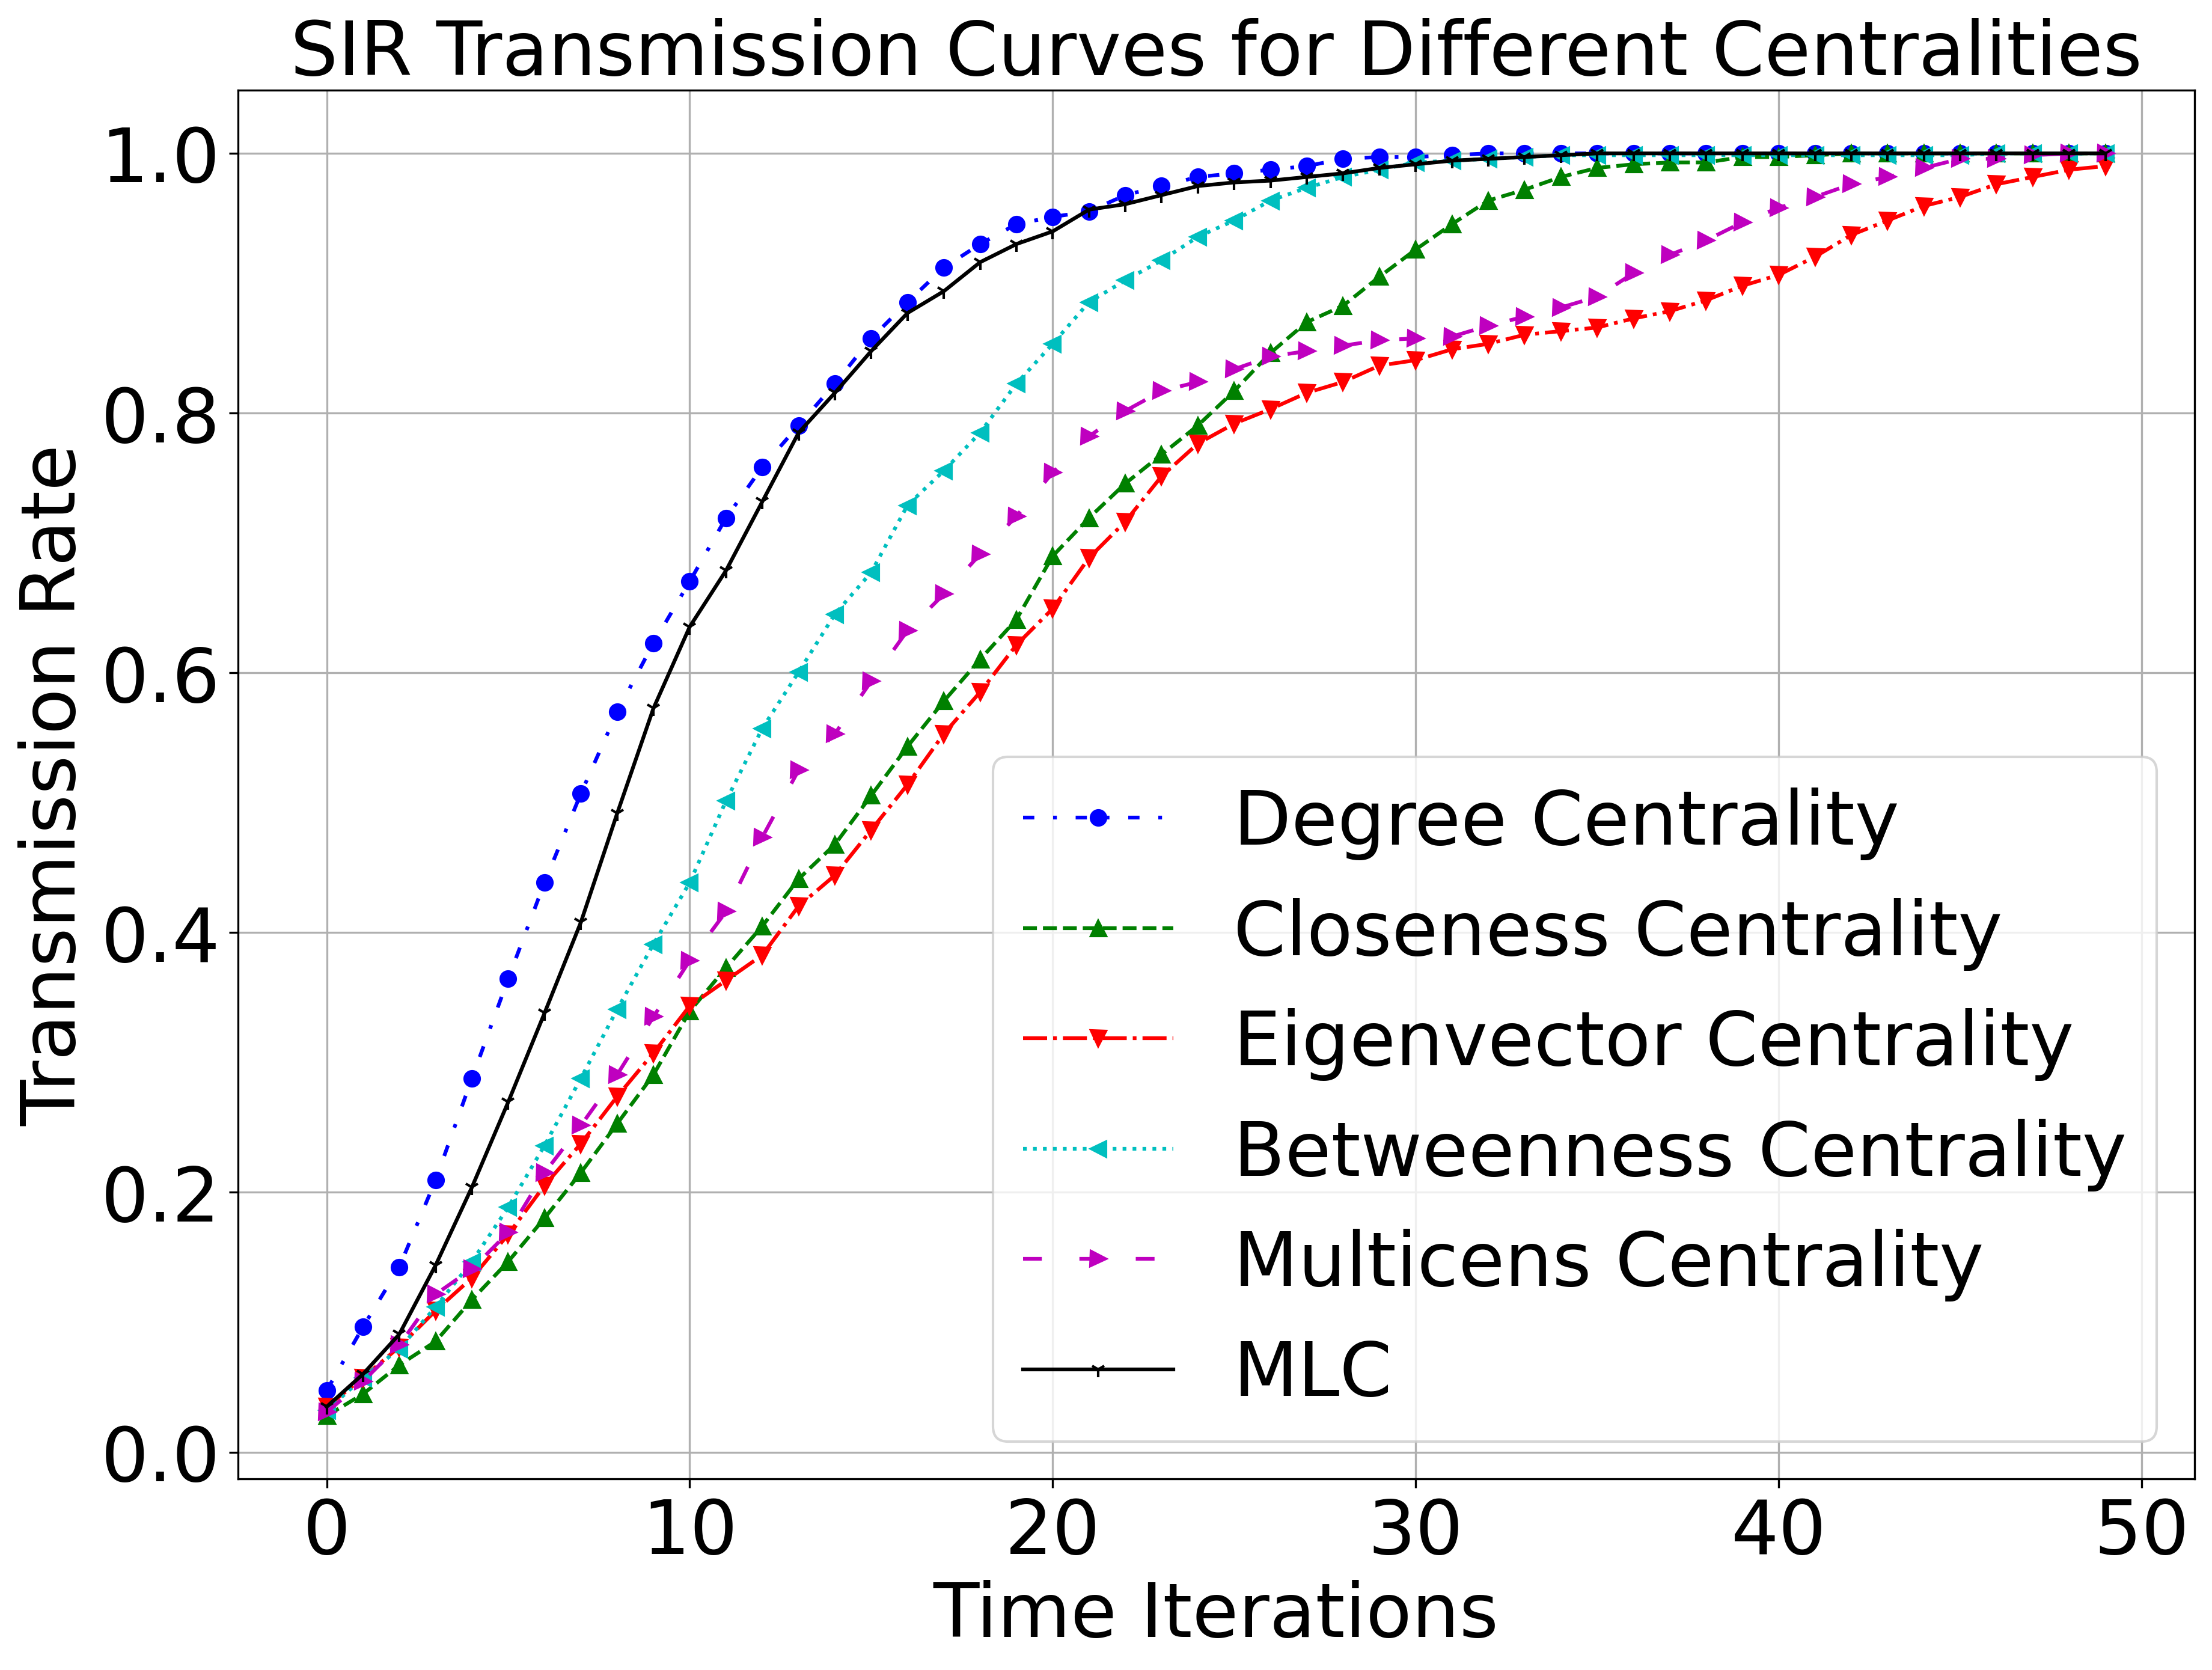
\includegraphics[width=\textwidth]{figs/fig20-hif2a_arnt-k1top2.png}
	\subcaption{}
\end{minipage}
\hspace{0.5cm}
\begin{minipage}[b]{0.25\linewidth}
	\centering
	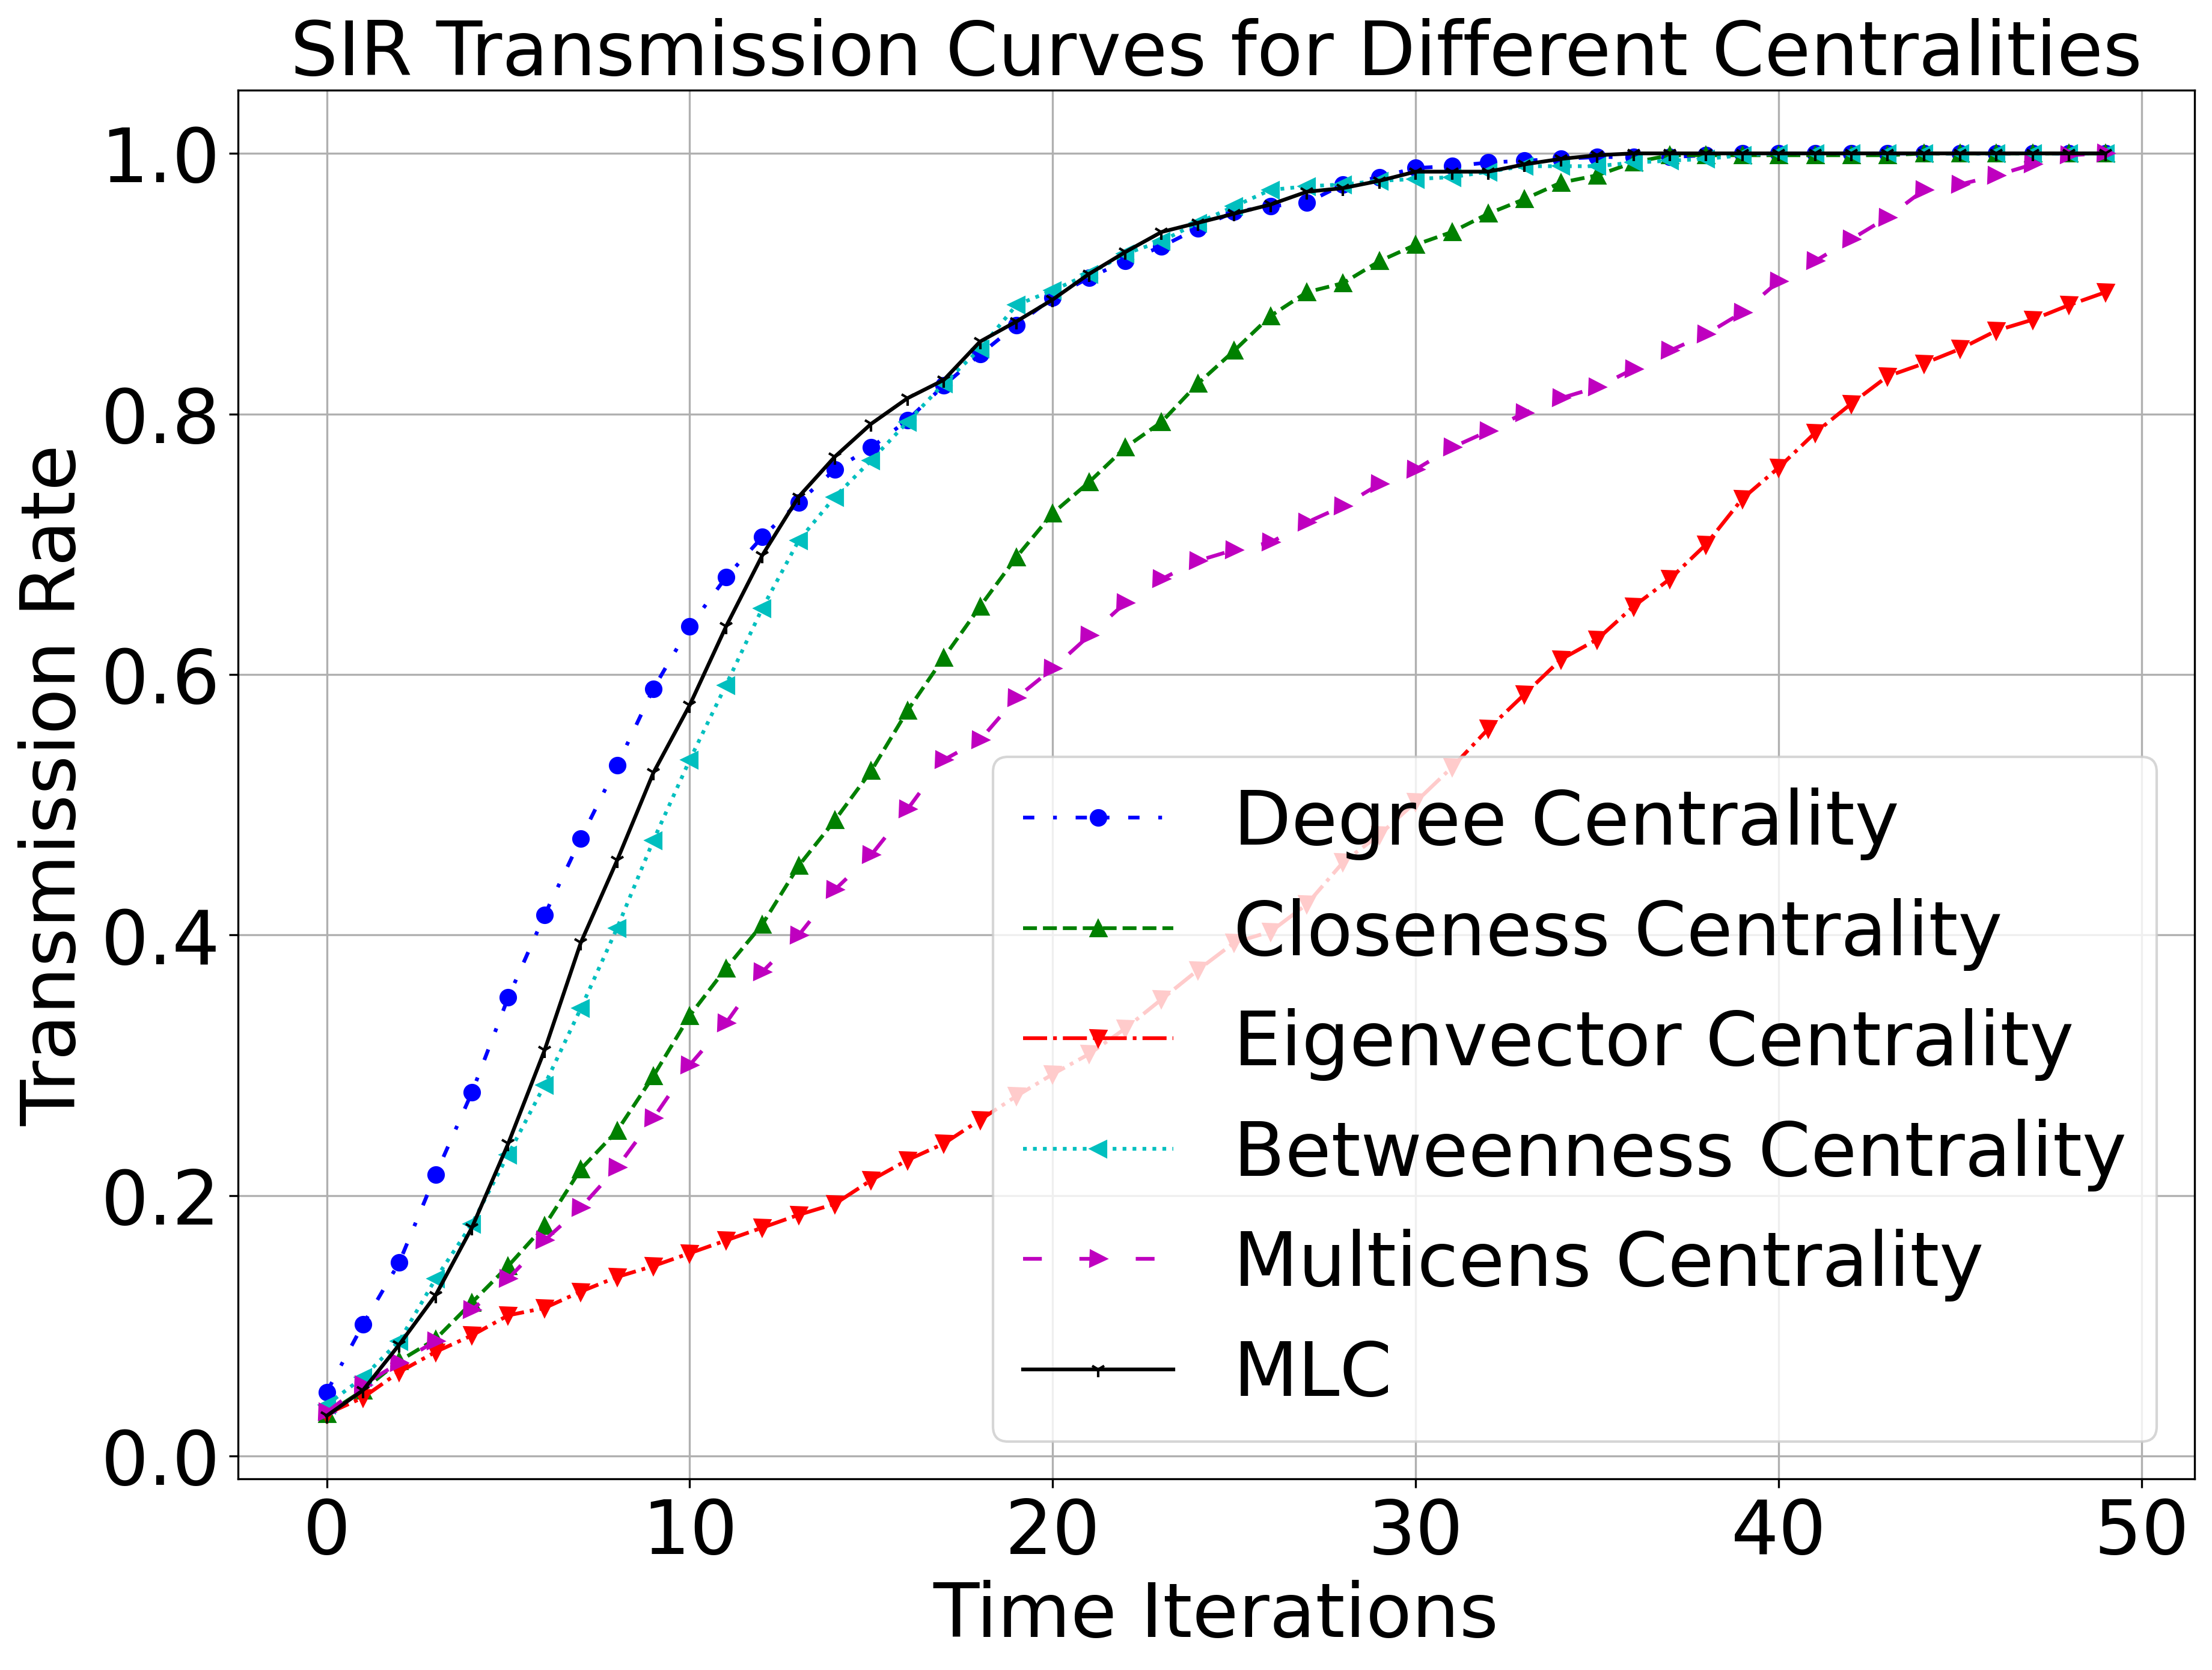
\includegraphics[width=\textwidth]{figs/fig21-hif3a_arnt-k2top2.png}
	\subcaption{}
\end{minipage}
\hspace{0.5cm}
\begin{minipage}[b]{0.25\linewidth}
	\centering
	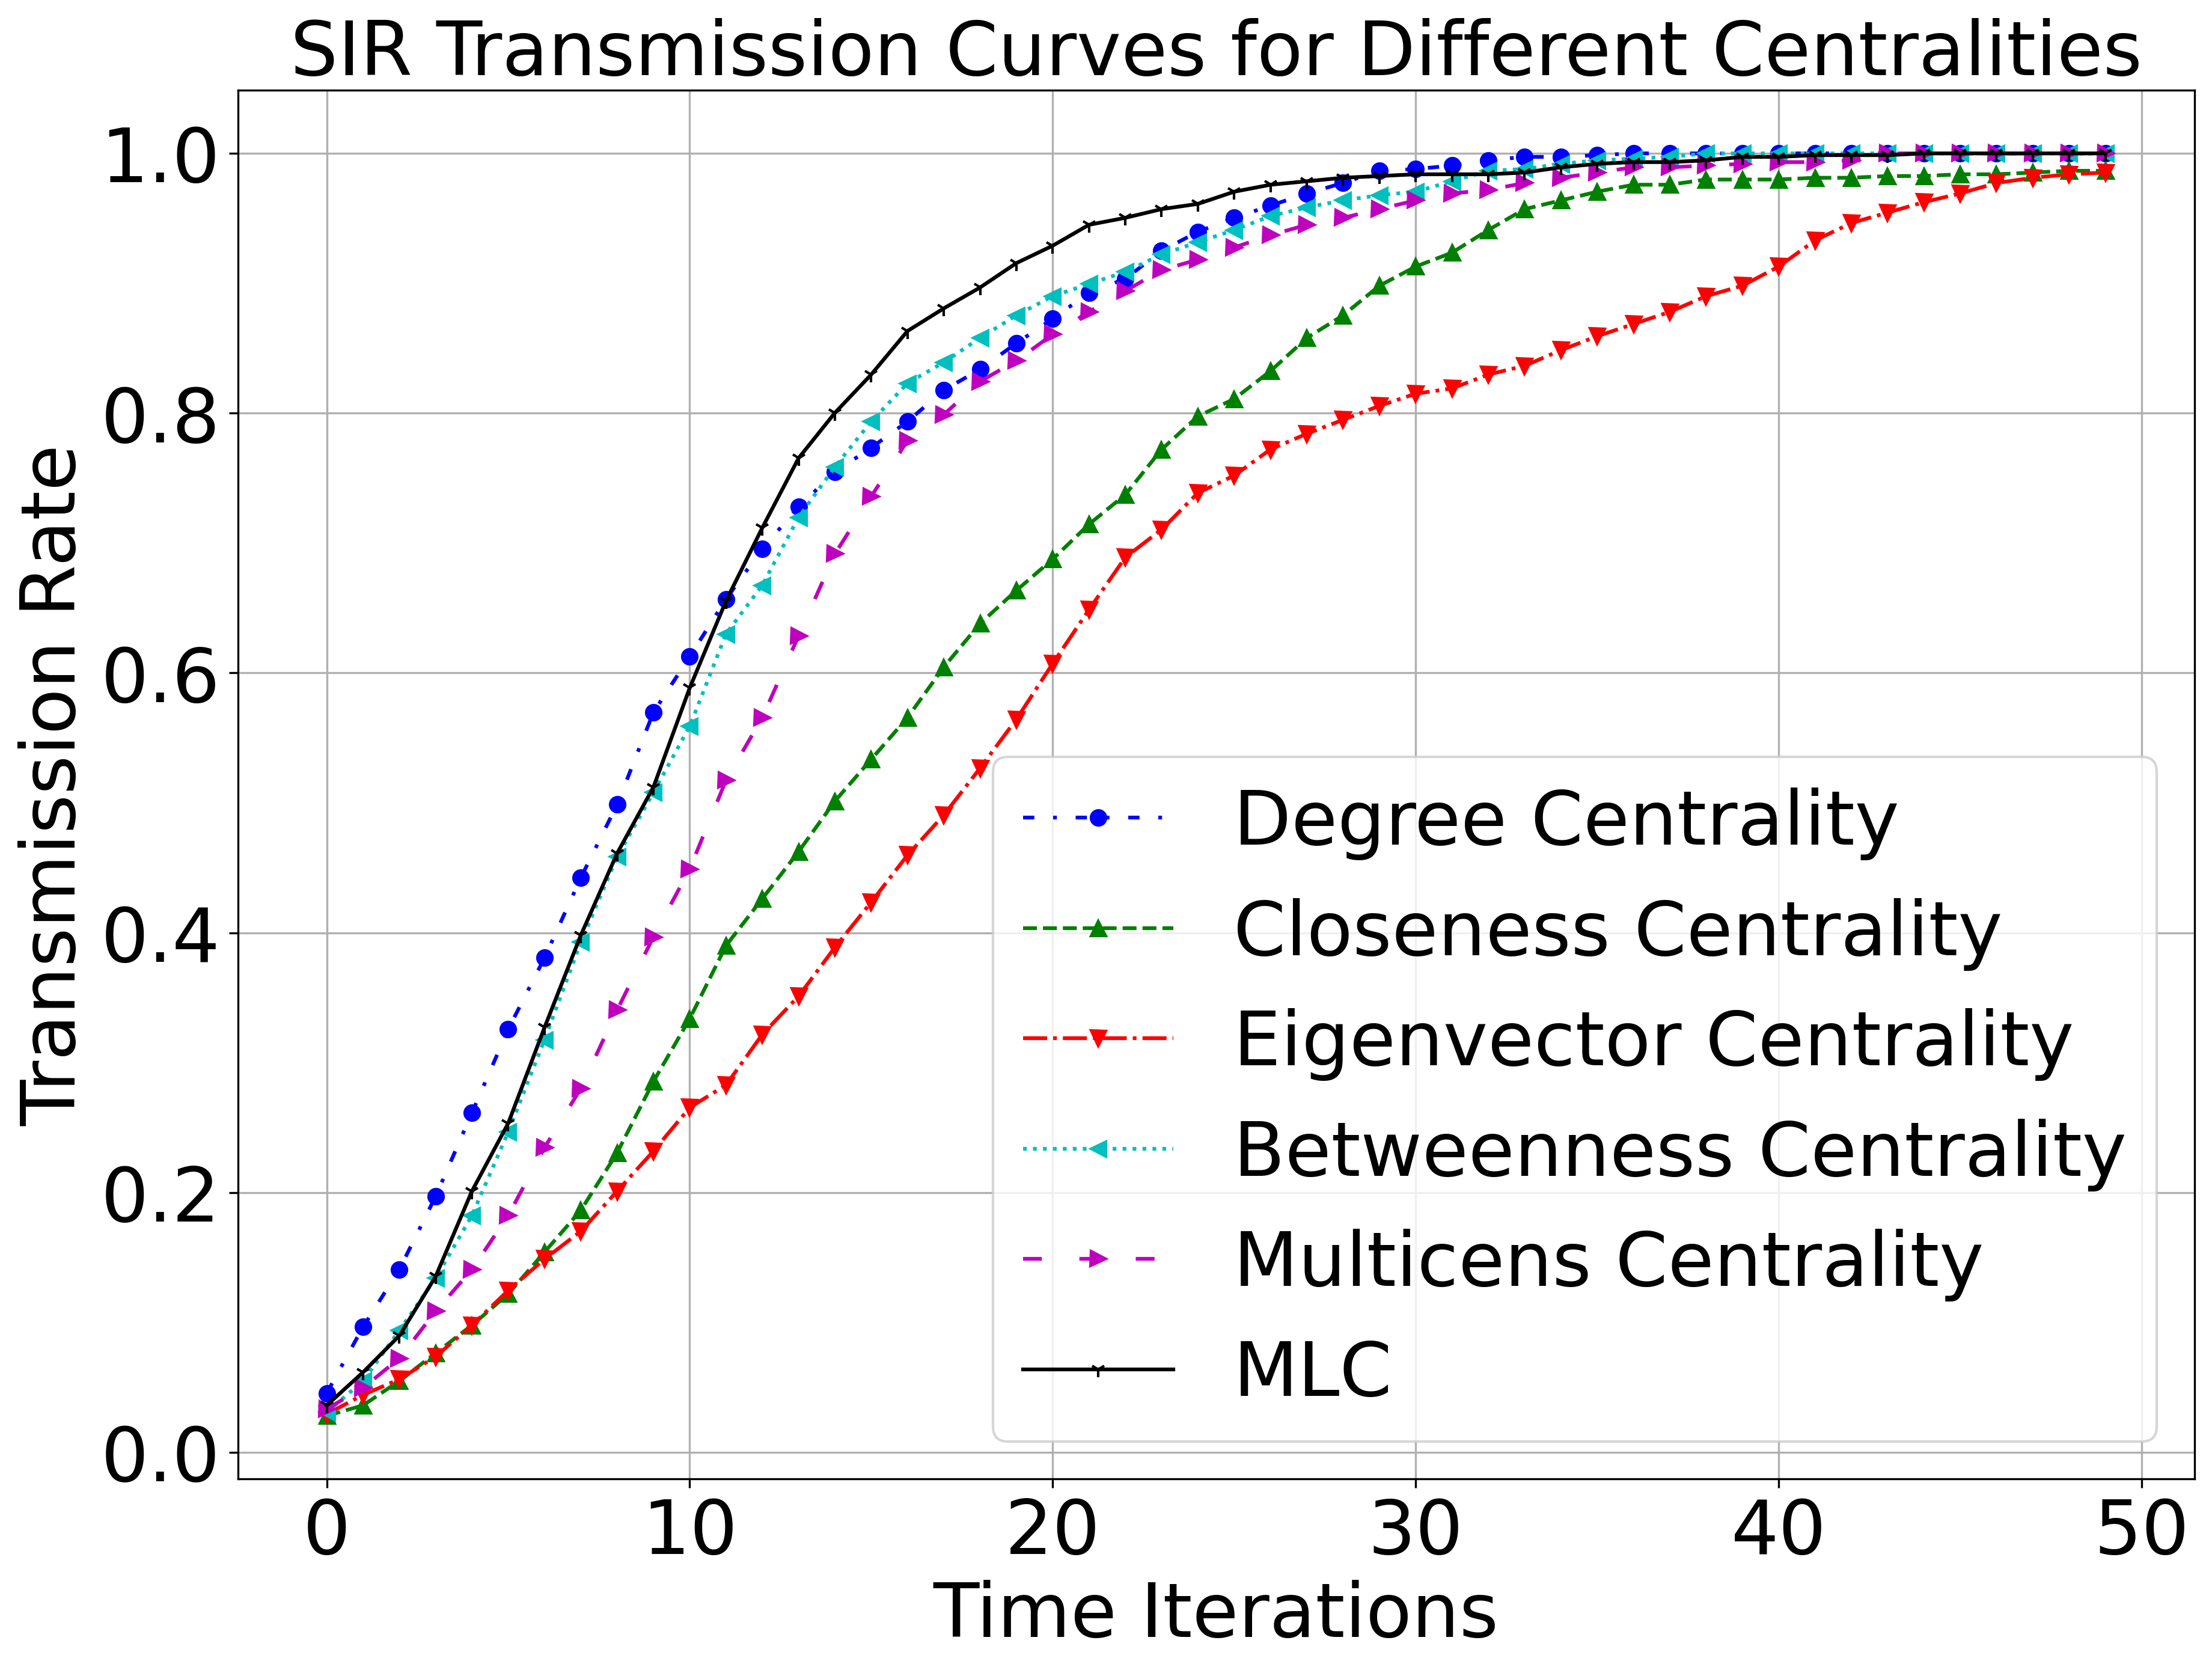
\includegraphics[width=\textwidth]{figs/fig22-npas1_arnt-k2top2.png}
	\subcaption{}
\end{minipage}

\vspace{0.5cm}

\begin{minipage}[b]{0.25\linewidth}
	\centering
	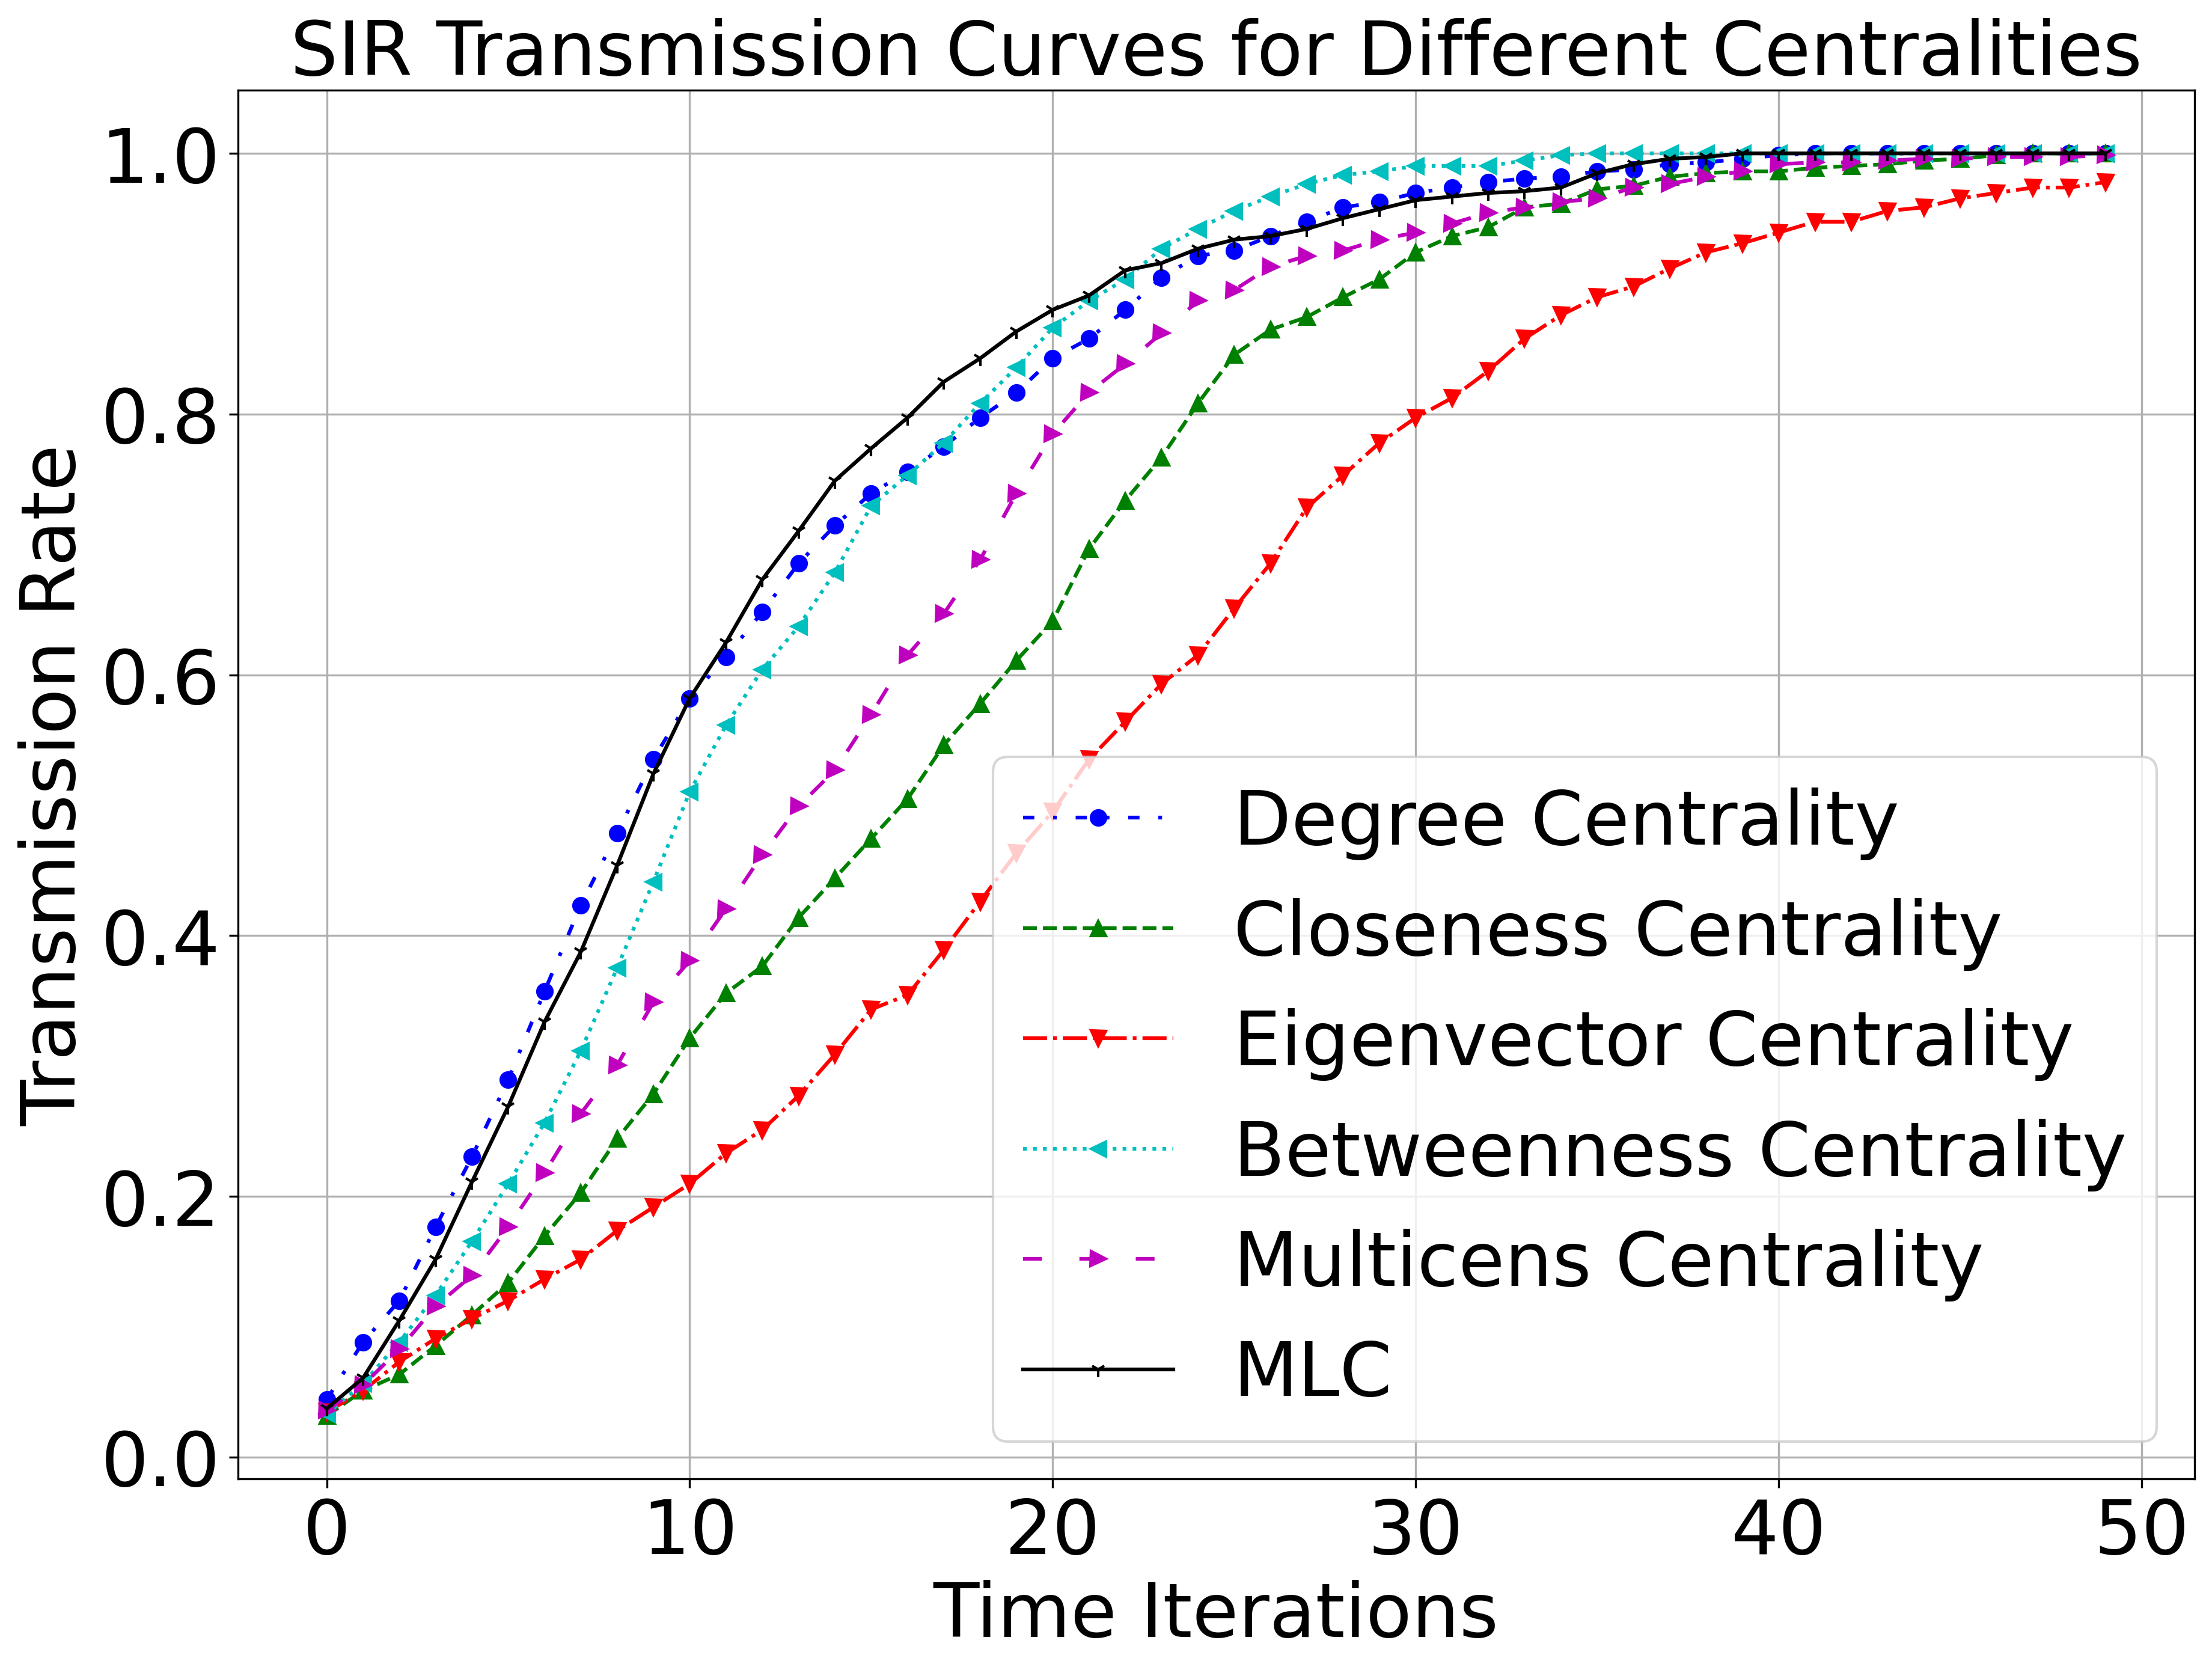
\includegraphics[width=\textwidth]{figs/fig23-npas2_bmal1-k2top2.png}
	\subcaption{}
\end{minipage}
\hspace{0.5cm}
\begin{minipage}[b]{0.25\linewidth}
	\centering
	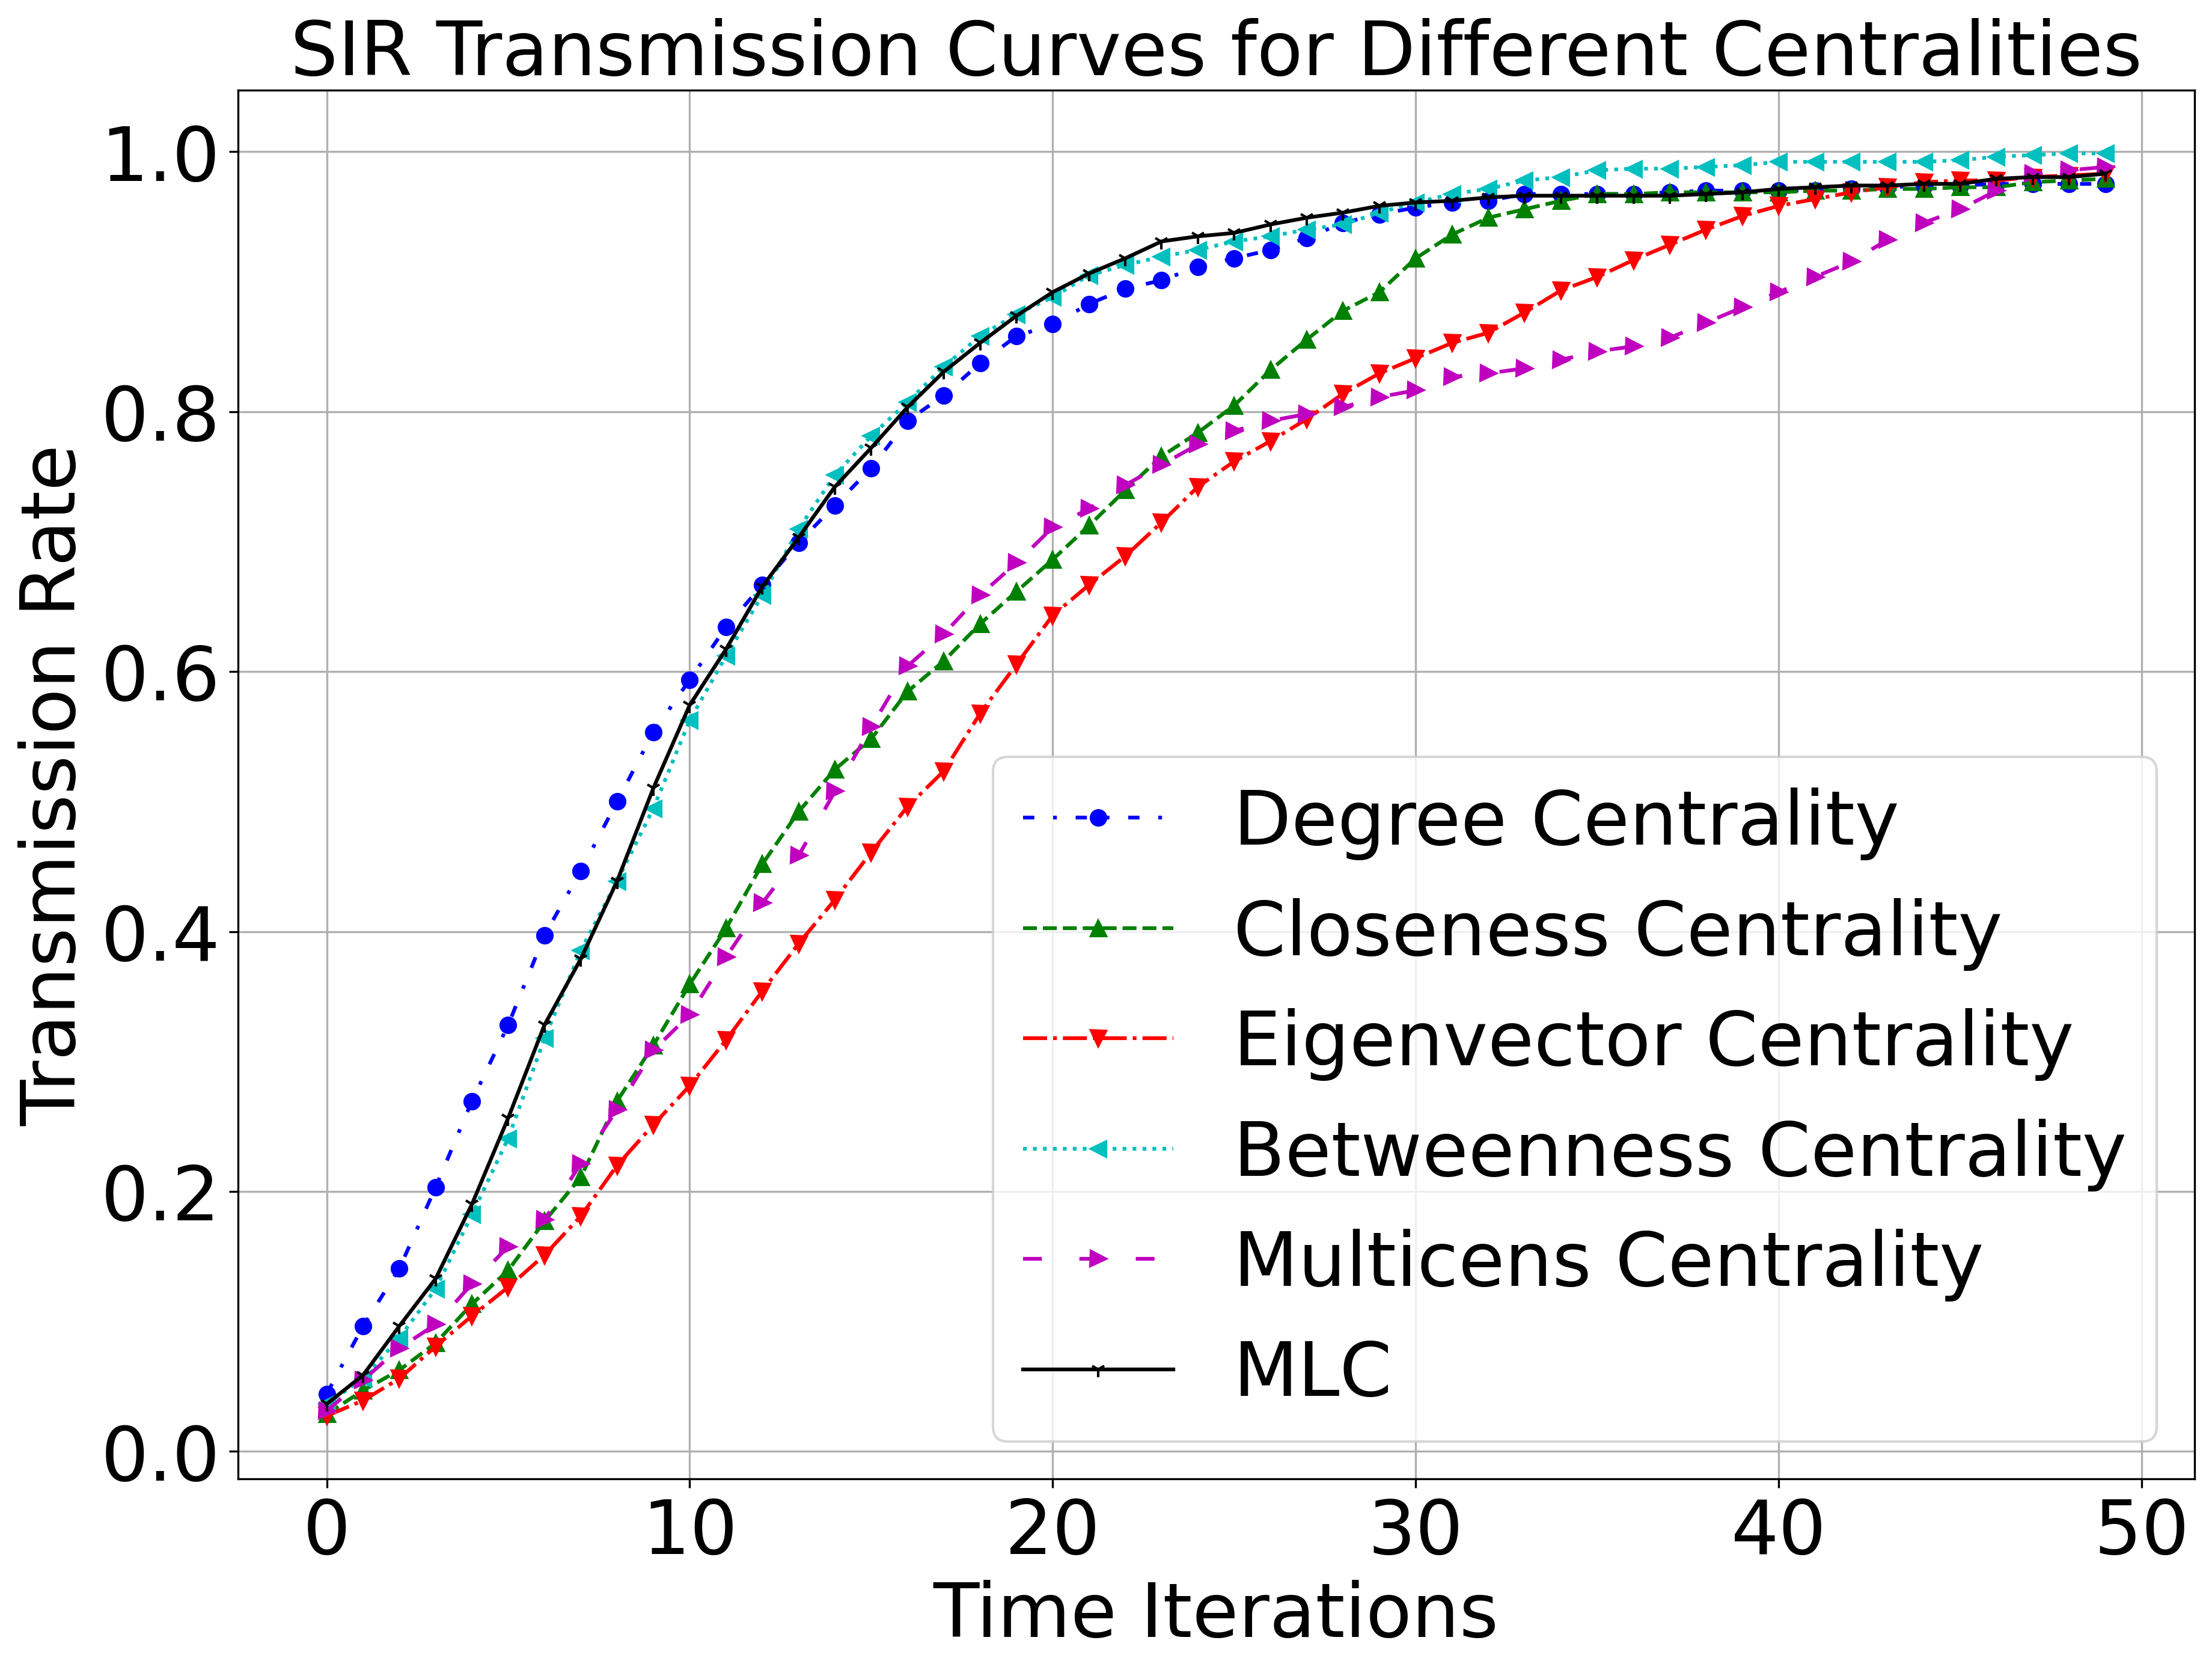
\includegraphics[width=\textwidth]{figs/fig24-npas3_arnt-k1top2.png}
	\subcaption{}
\end{minipage}
\hspace{0.5cm}
\begin{minipage}[b]{0.25\linewidth}
	\centering
	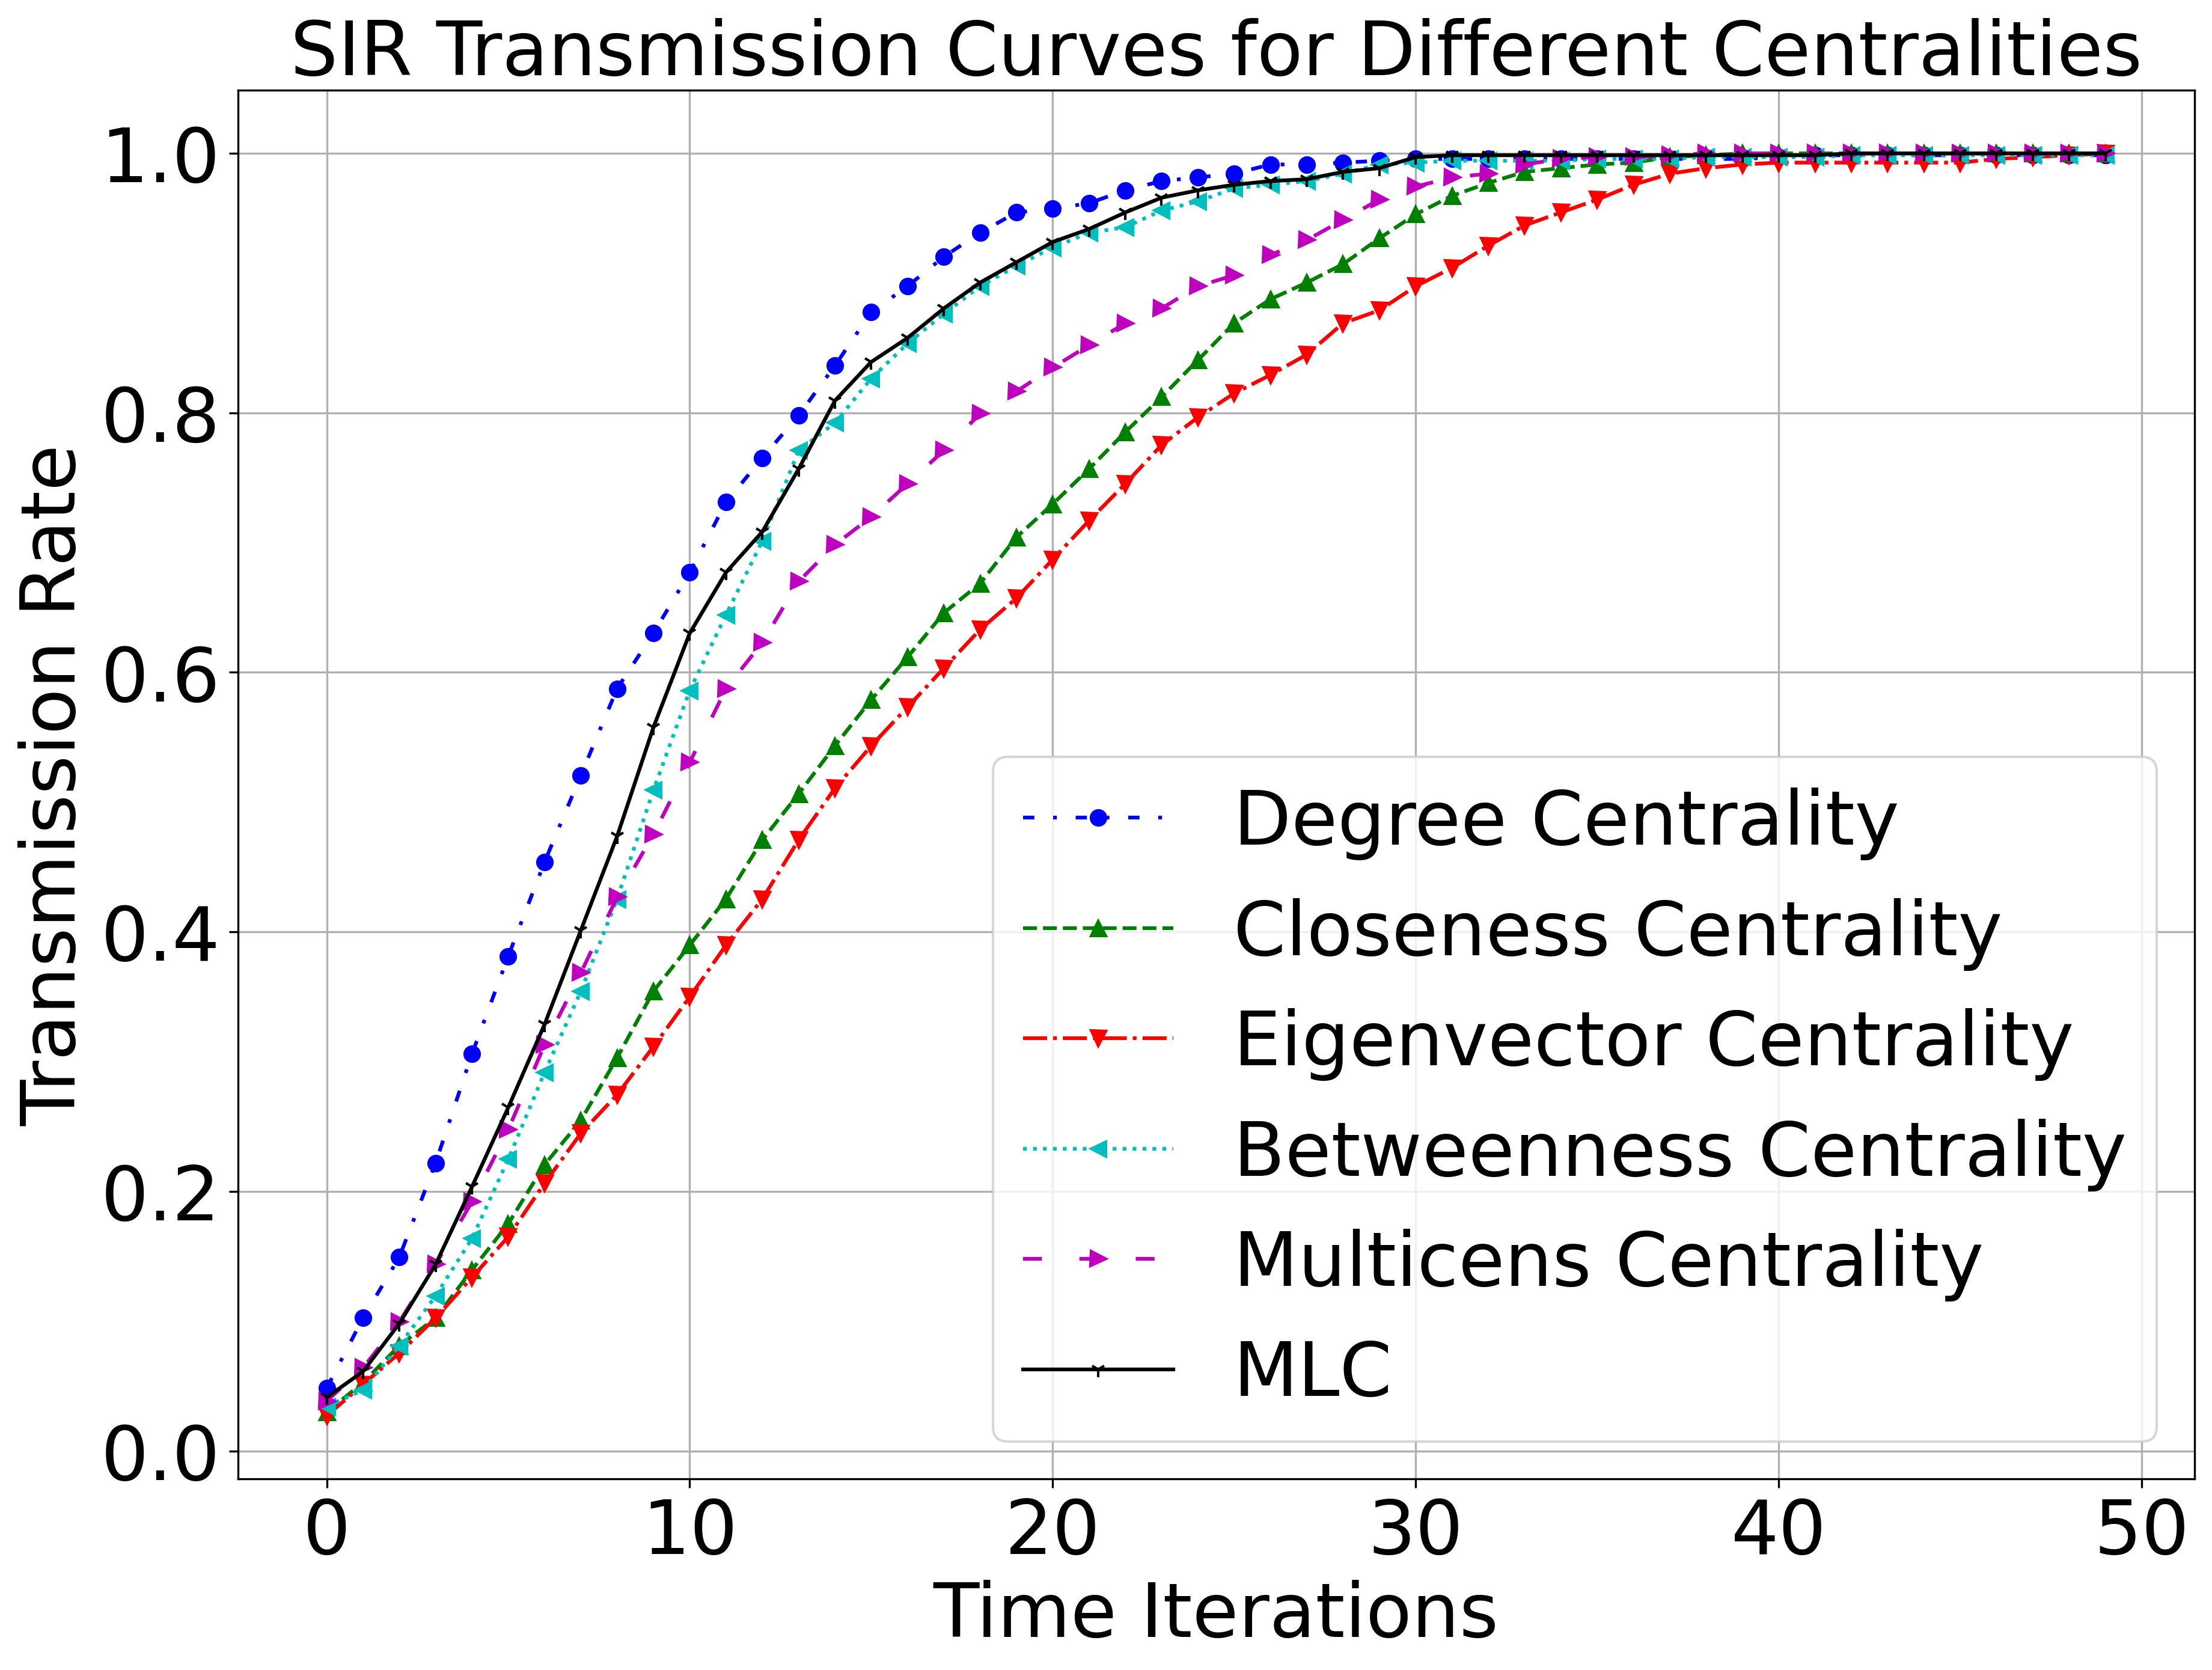
\includegraphics[width=\textwidth]{figs/fig25-npas4_arnt-k1top2.png}
	\subcaption{}
\end{minipage}

\vspace{0.5cm}

\begin{minipage}[b]{0.25\linewidth}
	\centering
	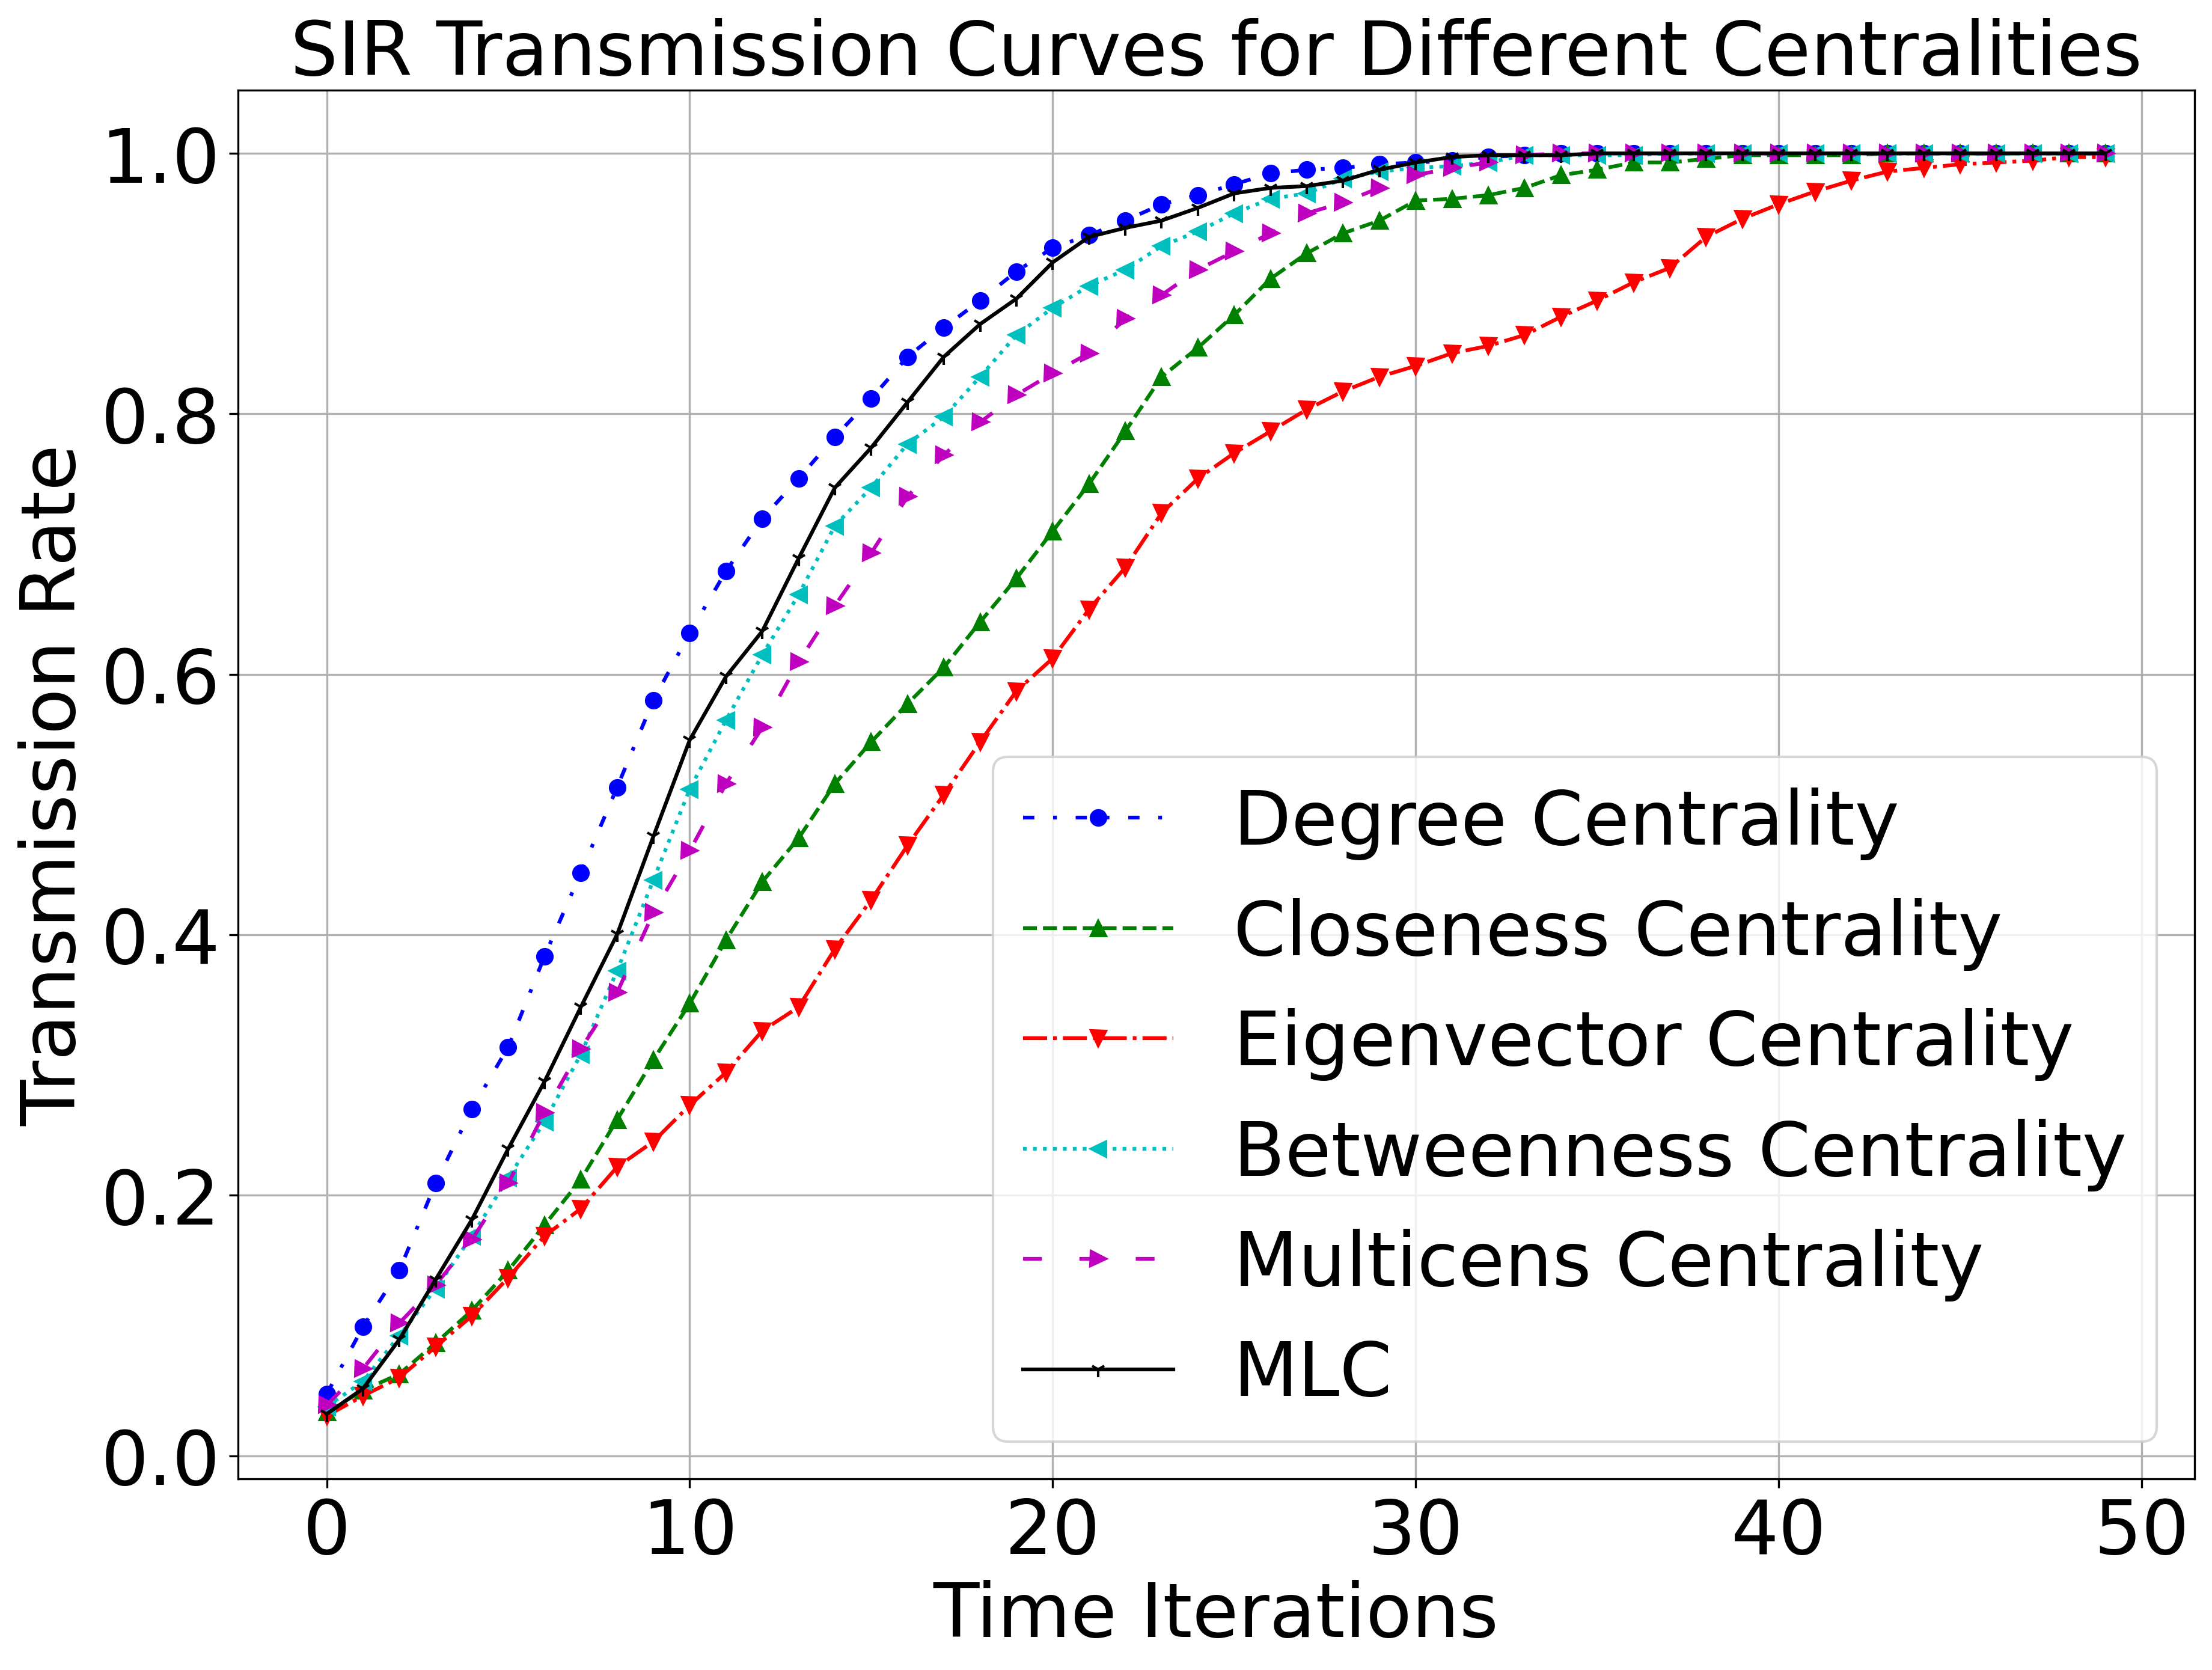
\includegraphics[width=\textwidth]{figs/fig26-sim1_arnt-k2top2.png}
	\subcaption{}
\end{minipage}
\hspace{0.5cm}
\begin{minipage}[b]{0.25\linewidth}
	\centering
	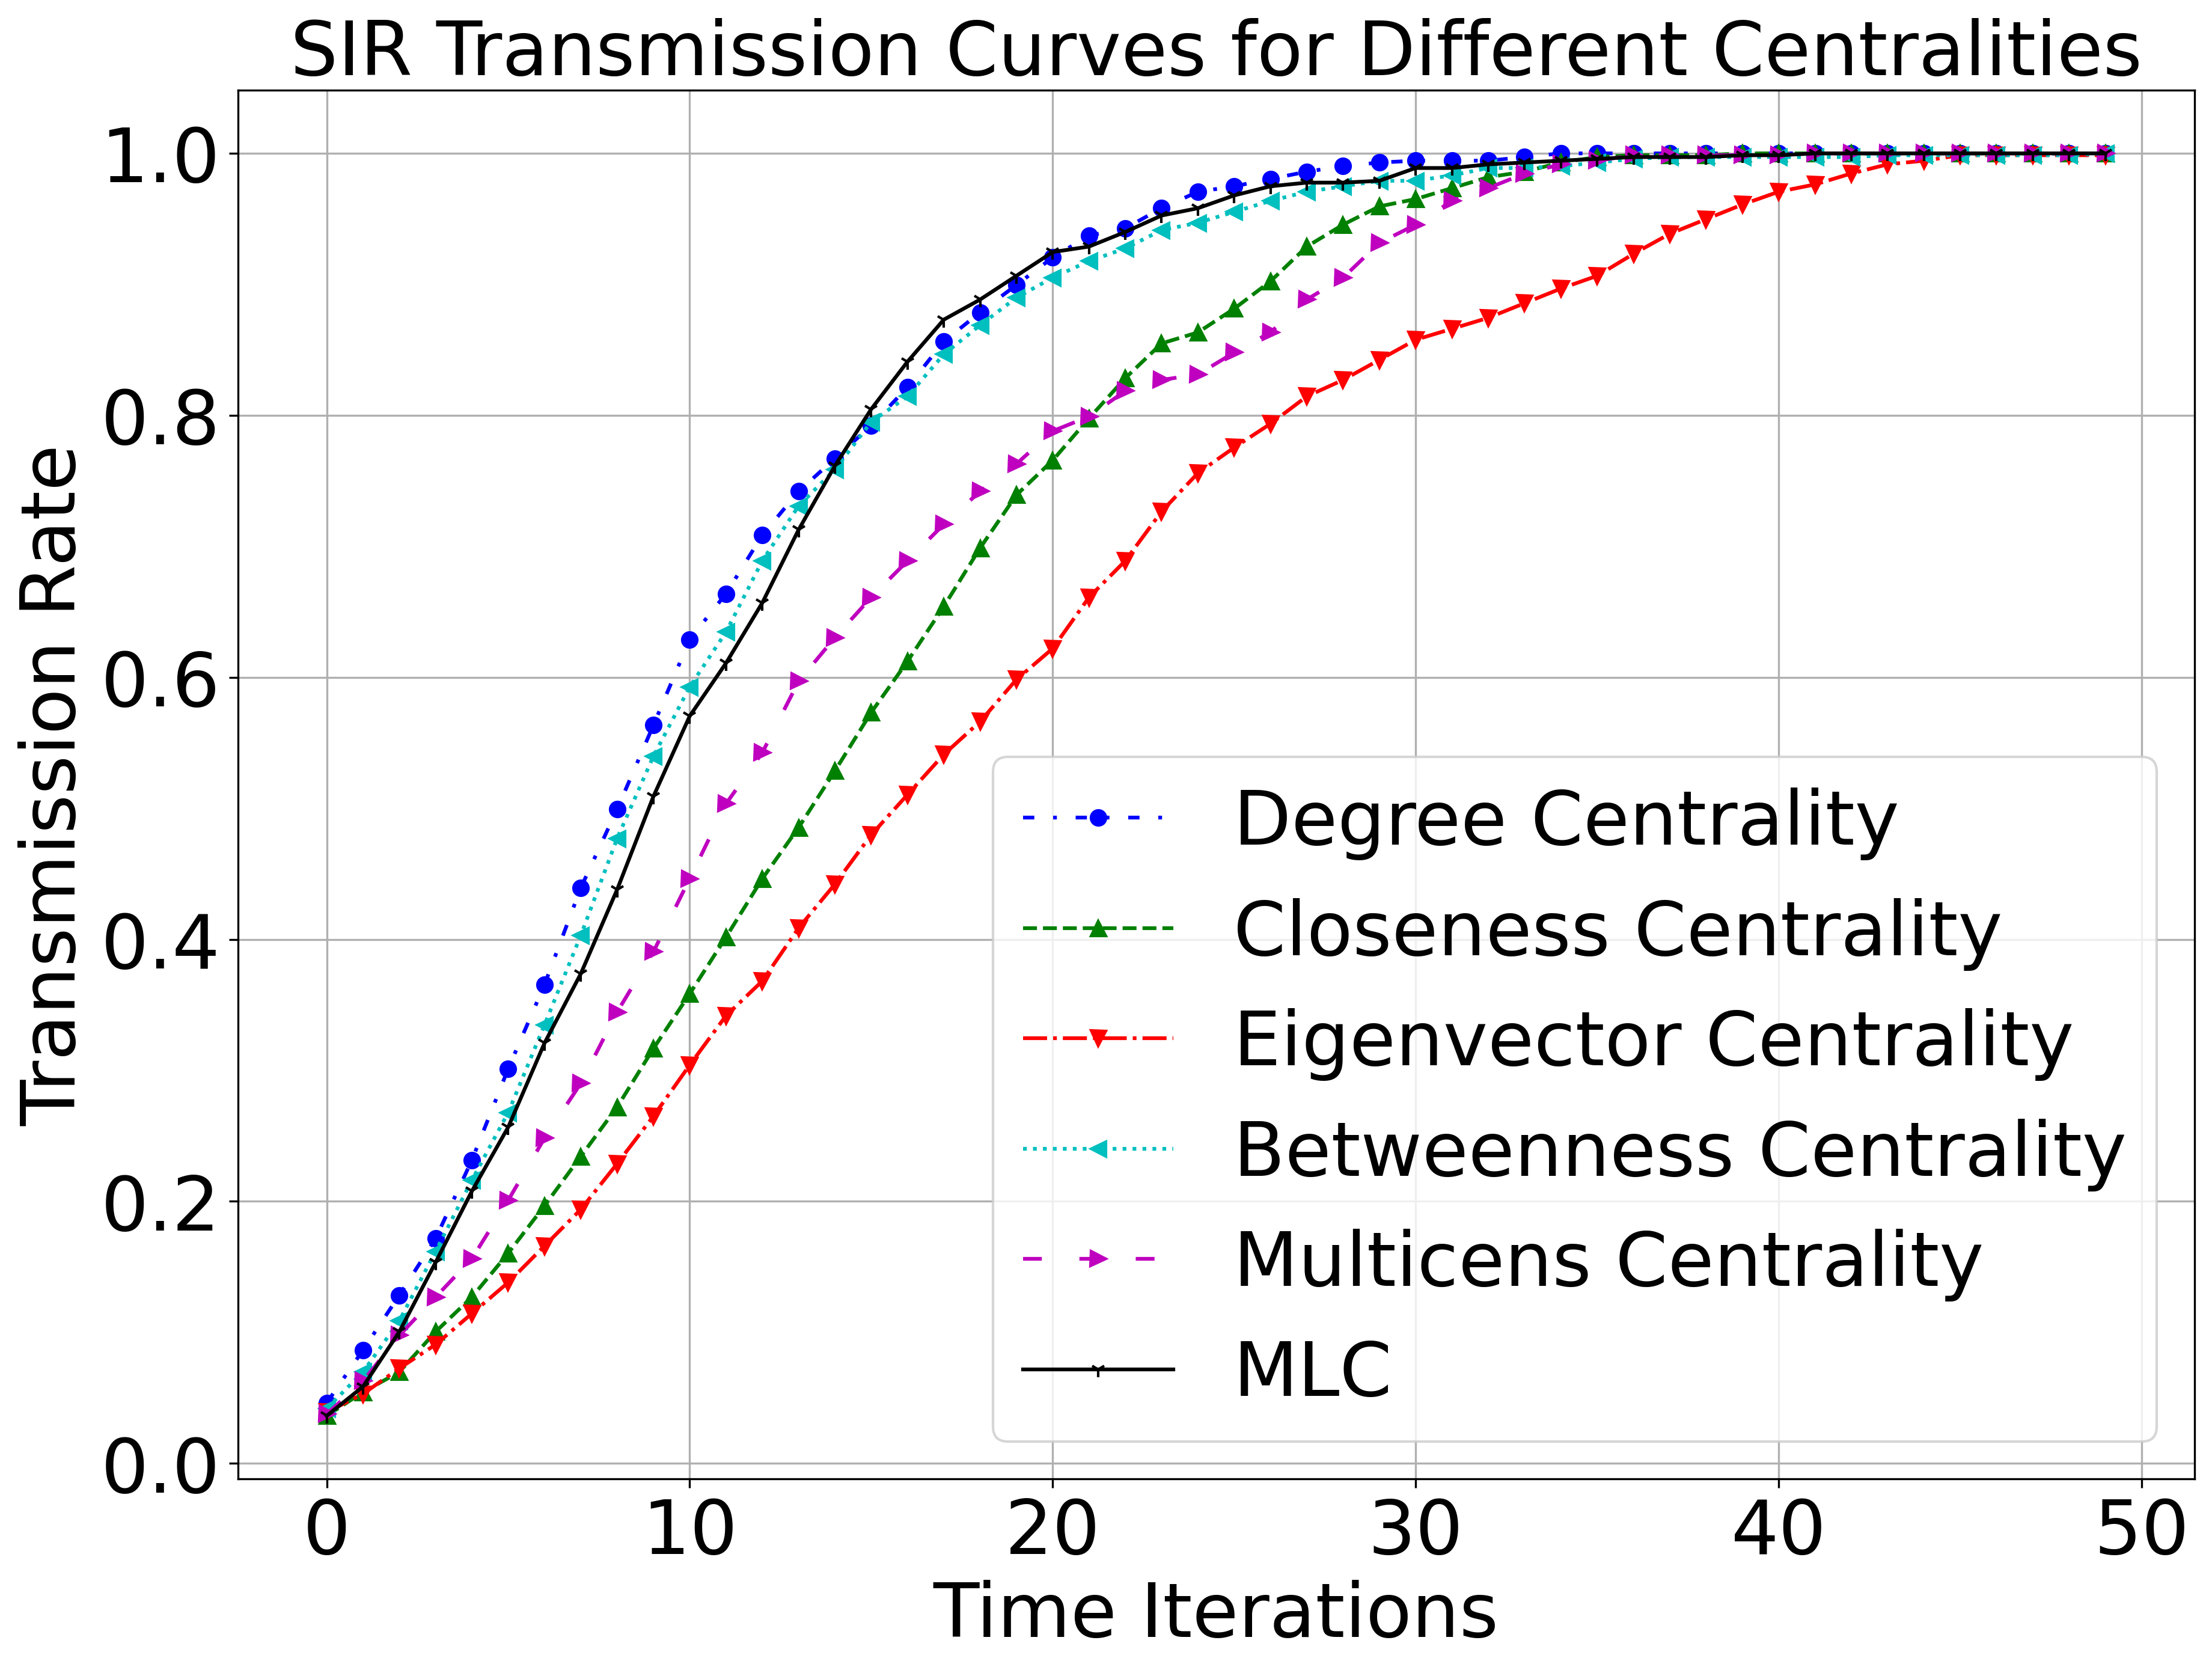
\includegraphics[width=\textwidth]{figs/fig27-sim2_arnt-k2top2.png}
	\subcaption{}
\end{minipage}

\caption{SIR transmission curves for degree, closeness, eigenvector, betweenness, multicens, and MLC centralities for proteins: (a) AHR-ARNT; (b) CLOCK-BMAL1; (c) HIF1A-ARNT; (d) HIF2A-ARNT; (e) HIF3A-ARNT; (f) NPAS1-ARNT; (g) NPAS2-BMAL1; (h) NPAS3-ARNT; (i) NPAS4-ARNT; (j) SIM1-ARNT; (k) SIM2-ARNT \label{fig:sir}}
\end{figure}

\section*{Discussion}
To evaluate the effectiveness of different centrality measures in determining the spread of an infectious disease, we utilize the Susceptible-Infected-Recovered (SIR) model~\cite{bailey1977theory,wang2011epidemics,feng2009networks}. The model operates on a network where nodes interact via edges, and disease transmission occurs probabilistically based on the network structure. Each node in the network can exist in one of three states: susceptible (S), not yet infected but vulnerable to infection; infected (I), currently infected and capable of spreading the disease; recovered (R), no longer infectious and immune to reinfection. The probability of infection is governed by the transmission rate $\beta$, while the probability of recovery is determined by $\gamma$. The infection propagates through the network over discrete time steps. 

To assess the role of centrality in transmission dynamics, we compare the impact of initializing infections in nodes ranked highest by various centrality measures: degree centrality, nodes with the highest number of direct connections; closeness centrality, nodes that have the shortest average path length to all others; eigenvector centrality, nodes that are well-connected to other influential nodes; betweenness centrality, nodes that frequently serve as intermediaries in shortest paths; multicens centrality, a composite measure incorporating multilayer centrality scores; multilayer centrality, centrality derived from interactions across multiple network layers.

For each centrality measure, the simulation follows these steps: {\it selecting initial infected nodes}, the top 2\% of nodes based on each centrality measure are chosen as the initial infected group; {\it disease transmission}, at each time step, infected nodes attempt to transmit the disease to their susceptible neighbors with probability $\beta = 0.1$; {\it recovery}, infected nodes recover with probability $\gamma = 0.1$ and can no longer transmit the disease; {\it tracking epidemic spread}, the fraction of infected nodes over time is recorded. The simulation is run for 50 time steps for each centrality measure to analyze how the infection propagates across the network.

Figure~\ref{fig:sir} presents the infection curves corresponding to different centrality measures for proteins: (a) AHR-ARNT; (b) CLOCK-BMAL1; (c) HIF1A-ARNT; (d) HIF2A-ARNT; (e) HIF3A-ARNT; (f) NPAS1-ARNT; (g) NPAS2-BMAL1; (h) NPAS3-ARNT; (i) NPAS4-ARNT; (j) SIM1-ARNT; (k) SIM2-ARNT. The key observations include: degree centrality results in rapid early-stage infection due to high connectivity of initially infected nodes resulting in high overall transmission rate; closeness centrality facilitates rapid disease spread across the entire network resulting in average transmission rate; eigenvector centrality causes sustained transmission as high-scoring nodes reinforce long-term infection spread which in the protein networks leads to poor transmission rate; betweenness centrality delays the initial infection peak but leads to widespread outbreaks due to its control over network pathways, leadings to relatively high transmission rate; multicens centrality exhibits a balanced spread pattern, combining aspects of individual centrality measures leading to average transmission rate; multilayer centrality (MLC) captures complex inter-layer interactions, altering the disease spread trajectory compared to single-layer measures leading to competitive transmission rates, higher than that achieved by most of the other centrality measures. 

Figure~\ref{fig:corr1} 

\begin{figure}[h!]
\centering
\begin{minipage}[b]{0.28\linewidth}
\centering
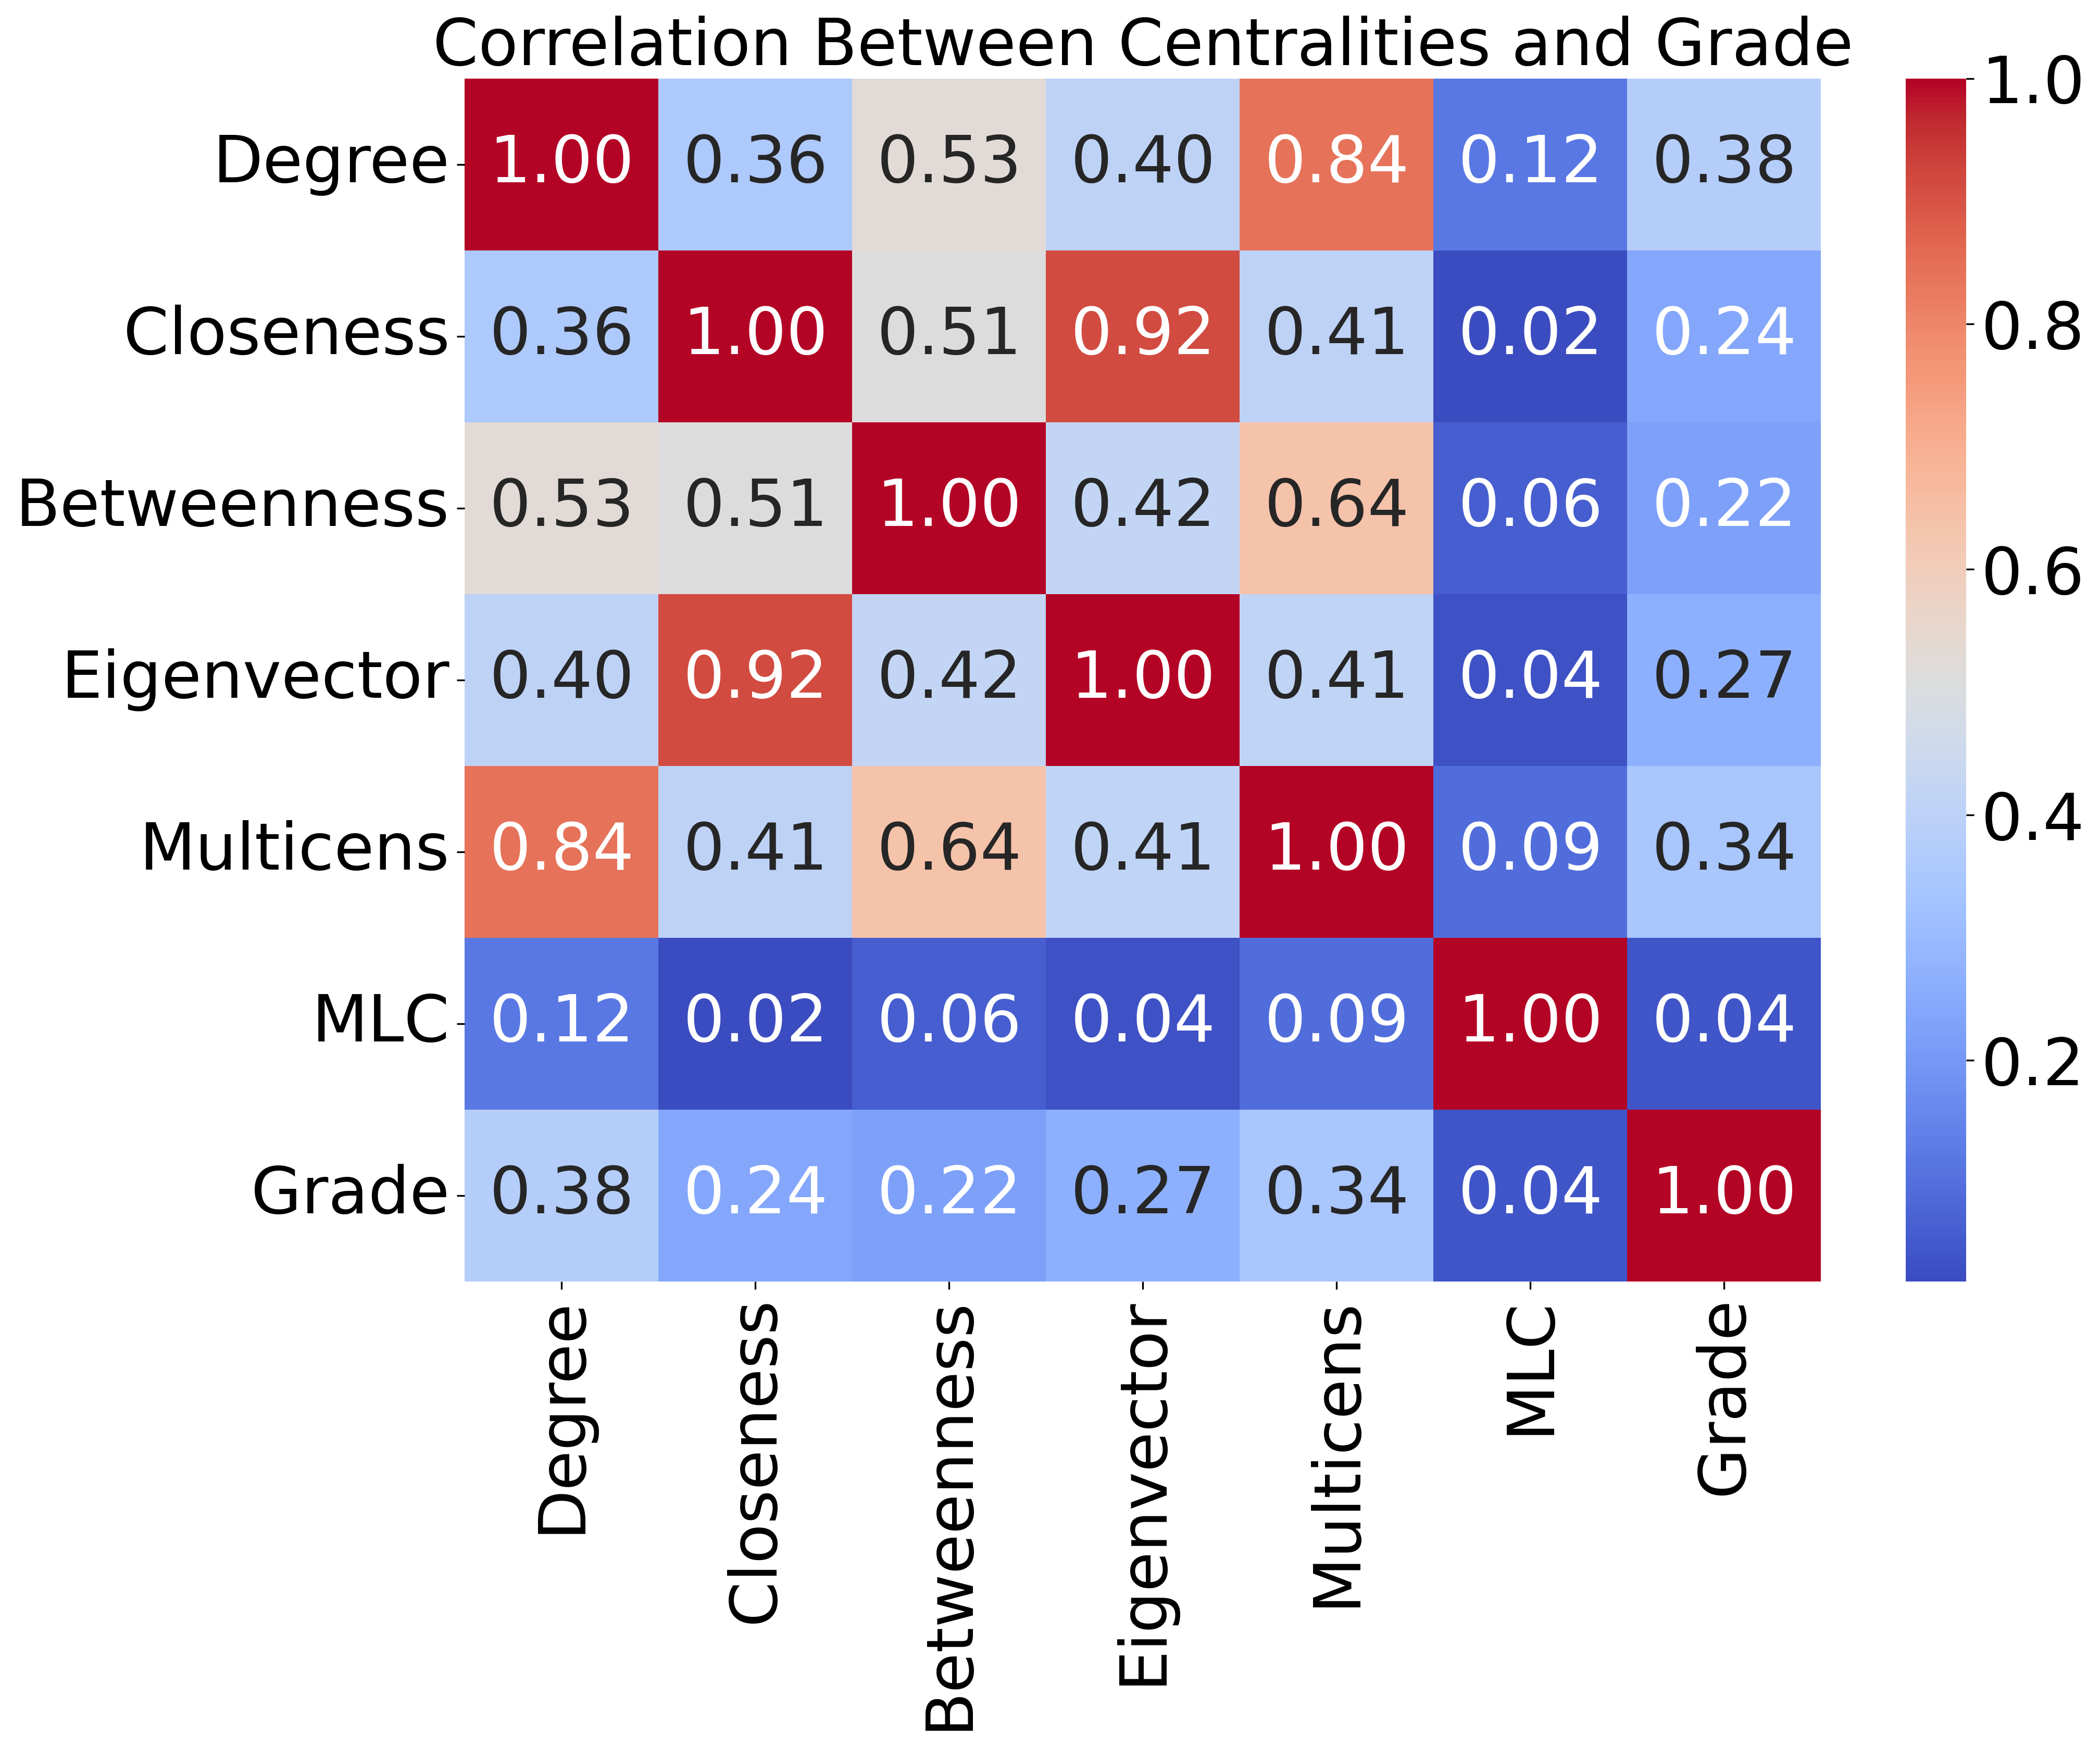
\includegraphics[width=\textwidth]{figs/fig28-ahr_arnt-corr.png}
\subcaption{}
\end{minipage}
\hspace{0.5cm}
\begin{minipage}[b]{0.28\linewidth}
\centering
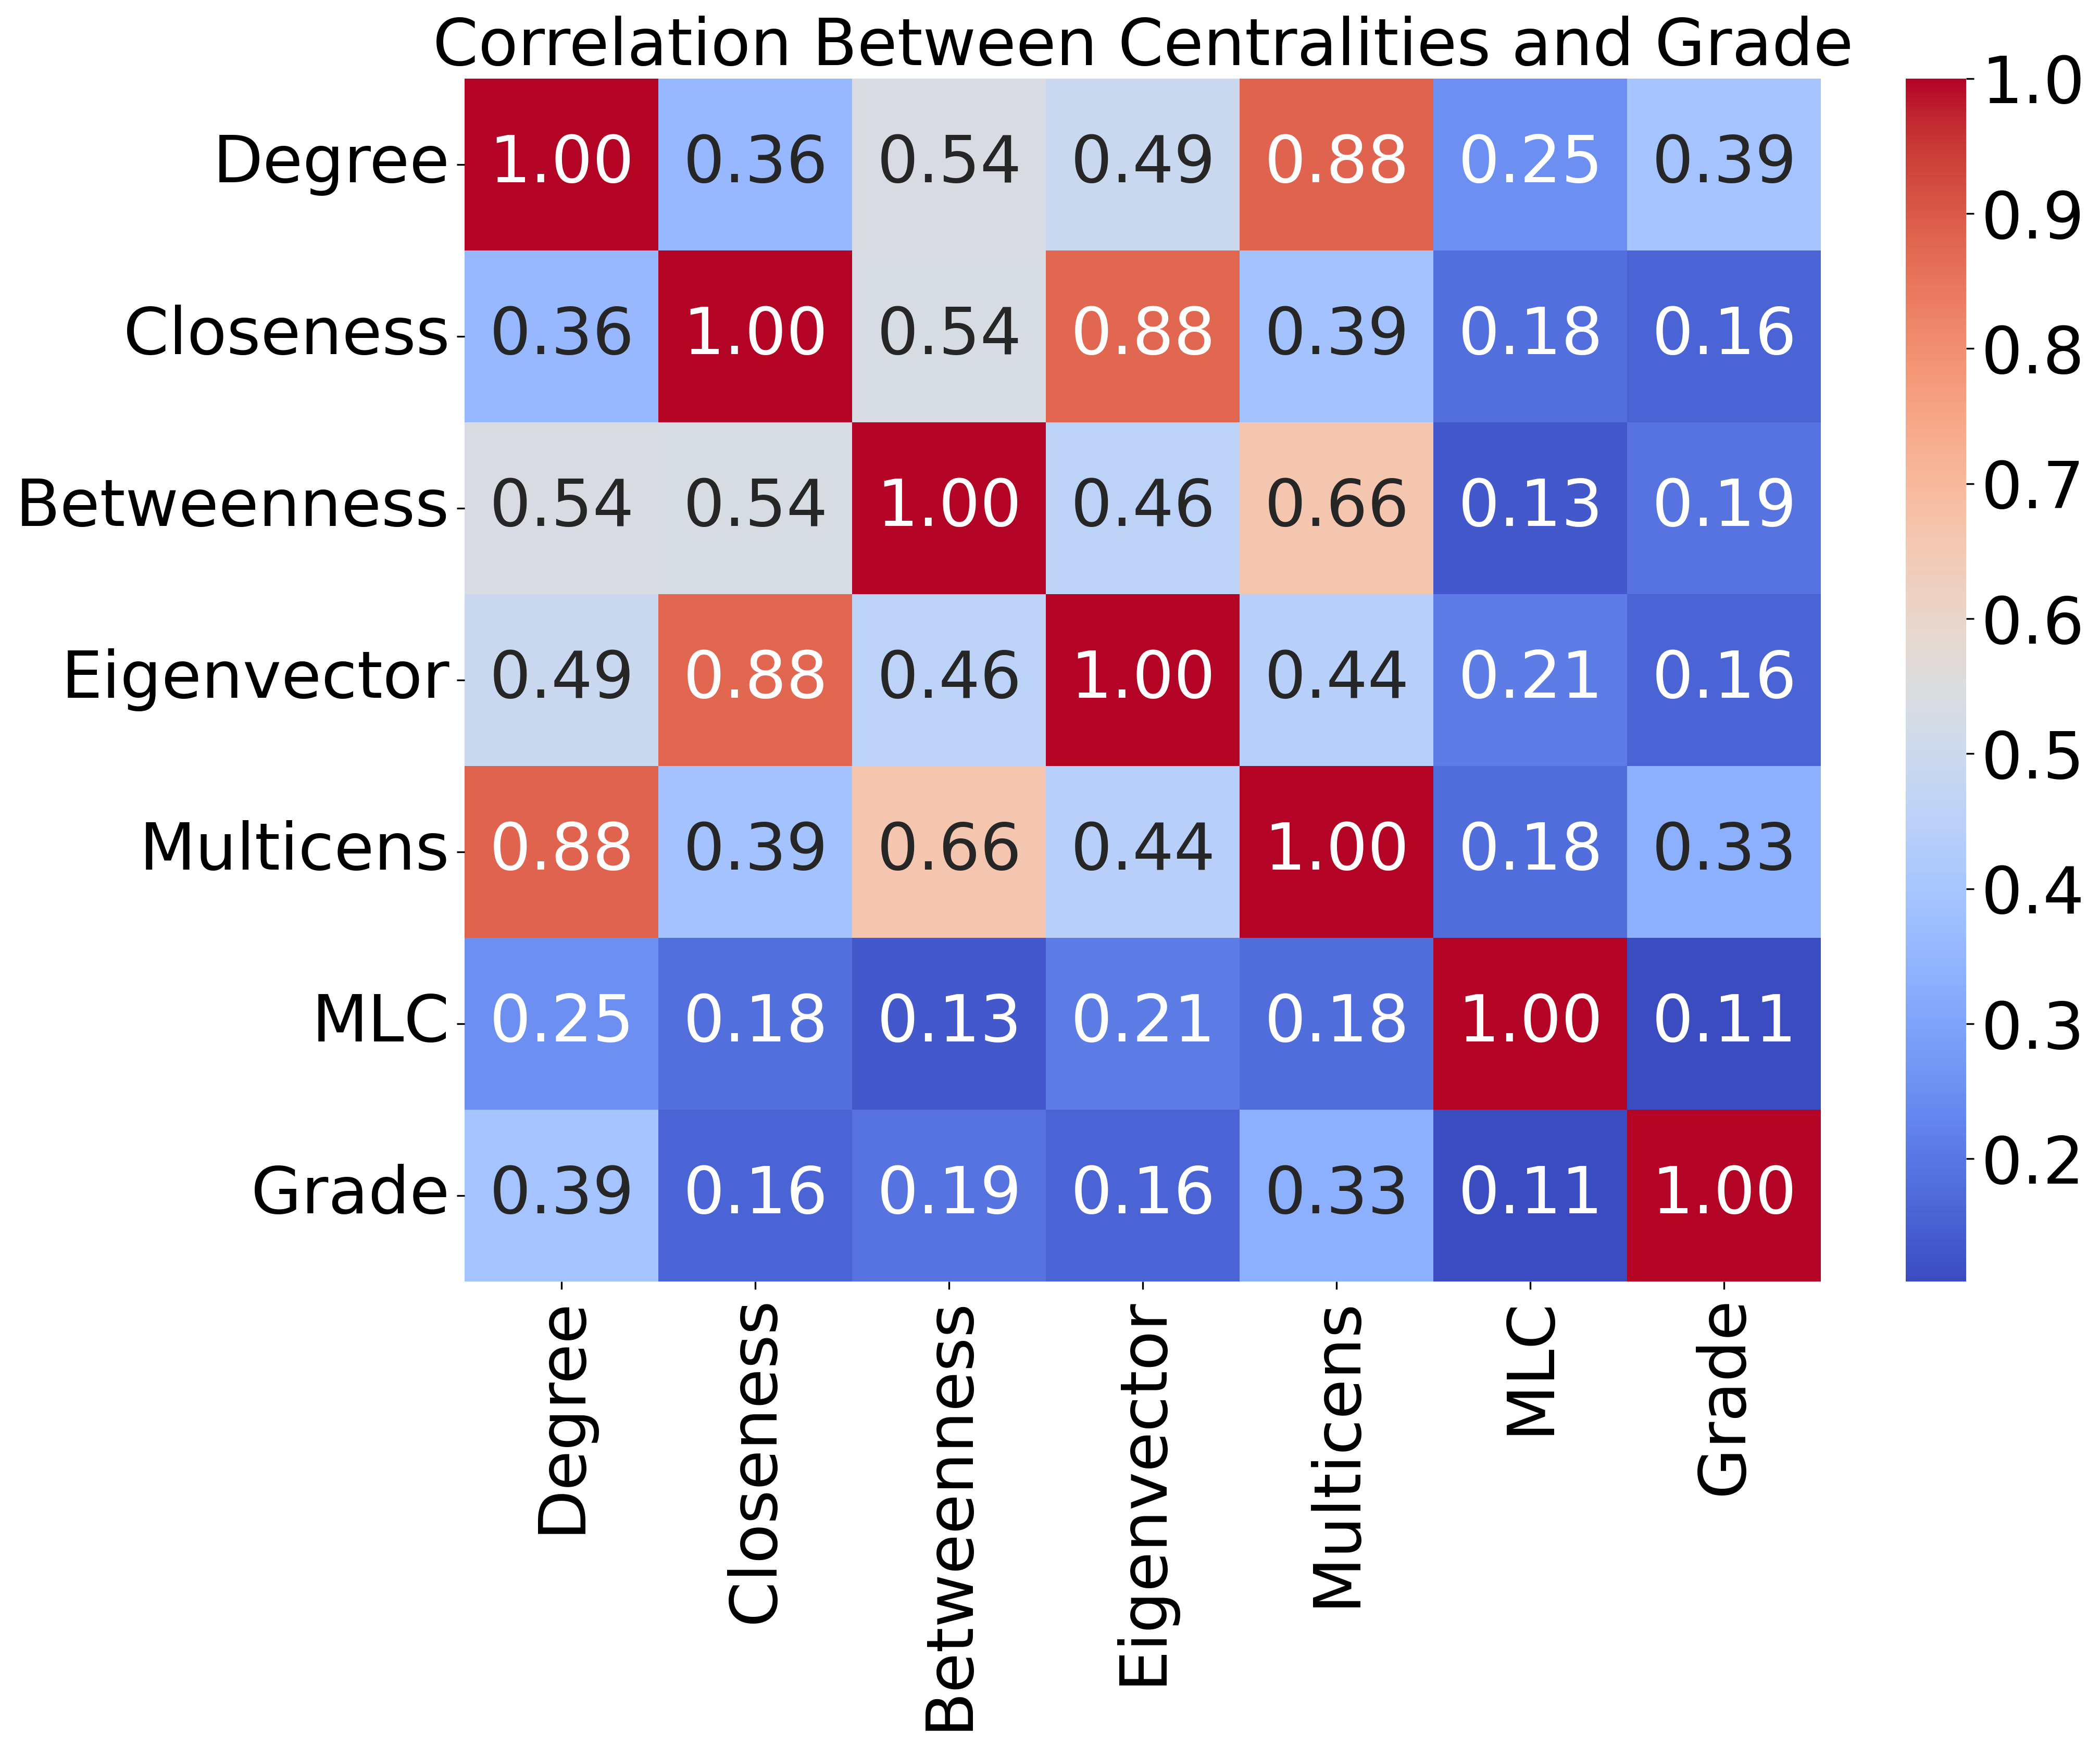
\includegraphics[width=\textwidth]{figs/fig29-clock_bmal1-corr.png}
\subcaption{}
\end{minipage}
\hspace{0.5cm}
\begin{minipage}[b]{0.28\linewidth}
\centering
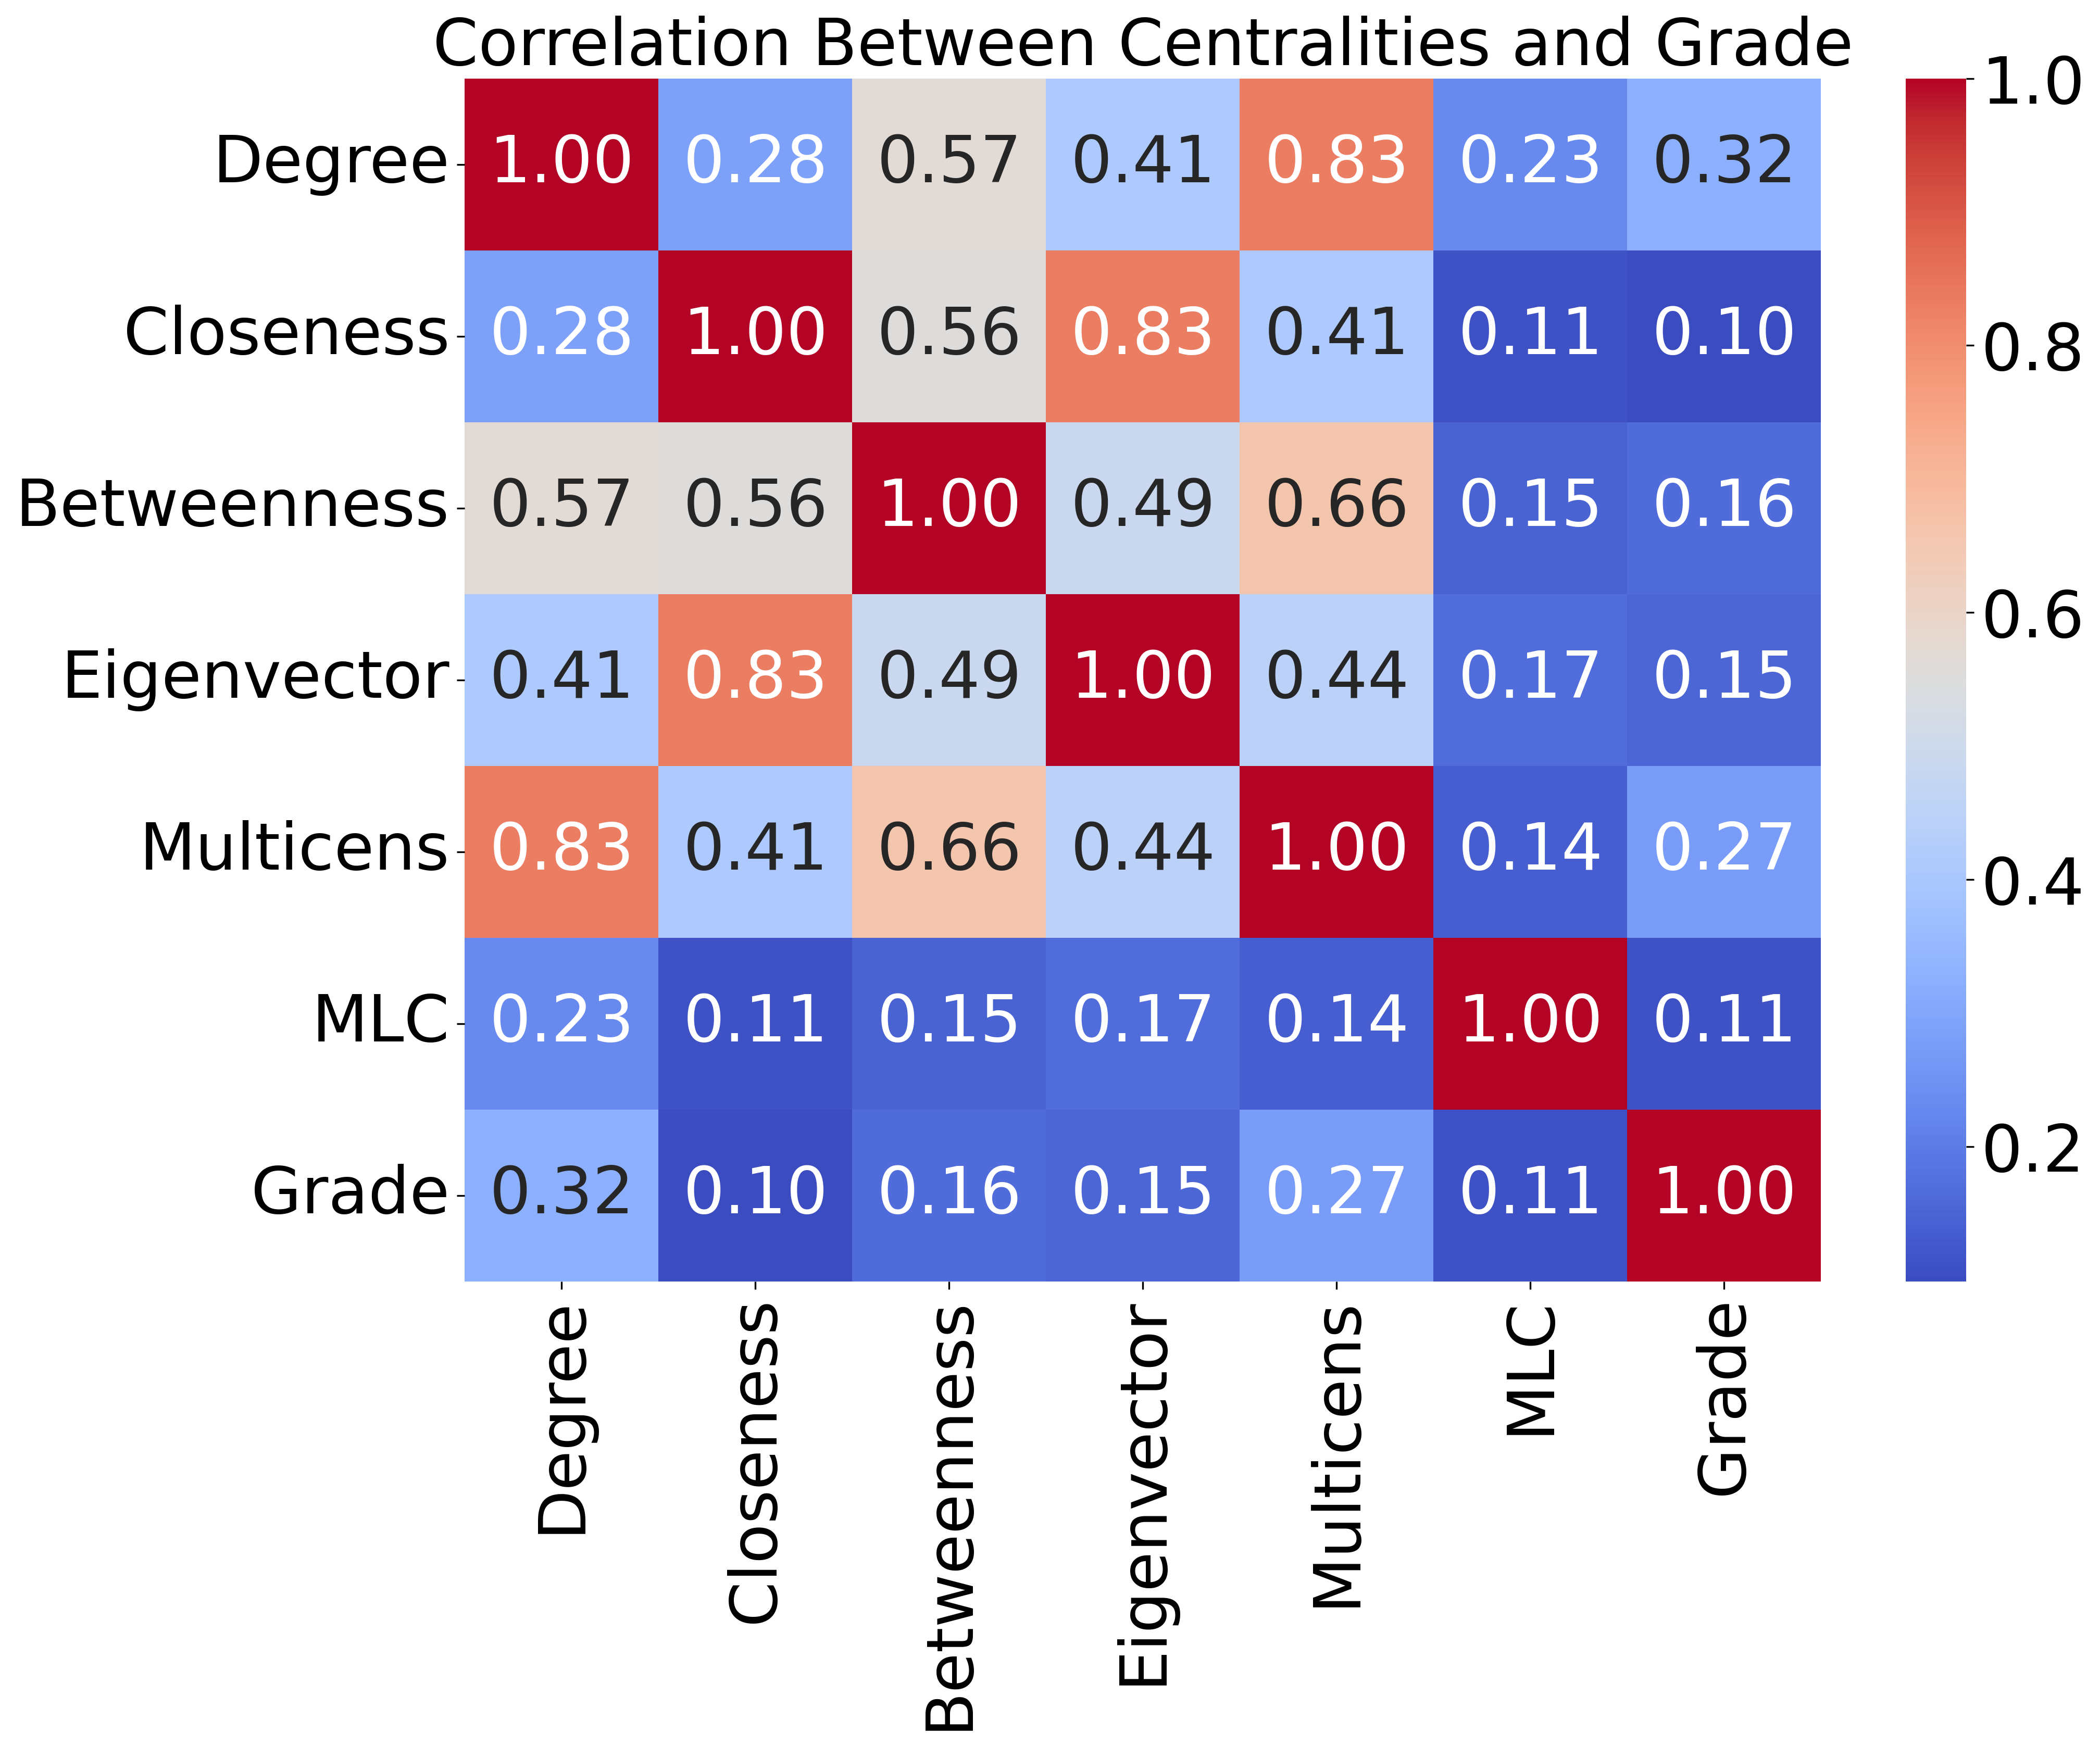
\includegraphics[width=\textwidth]{figs/fig30-hif1a_arnt-corr.png}
\subcaption{}
\end{minipage}


\vspace{0.5cm}

\begin{minipage}[b]{0.28\linewidth}
	\centering
	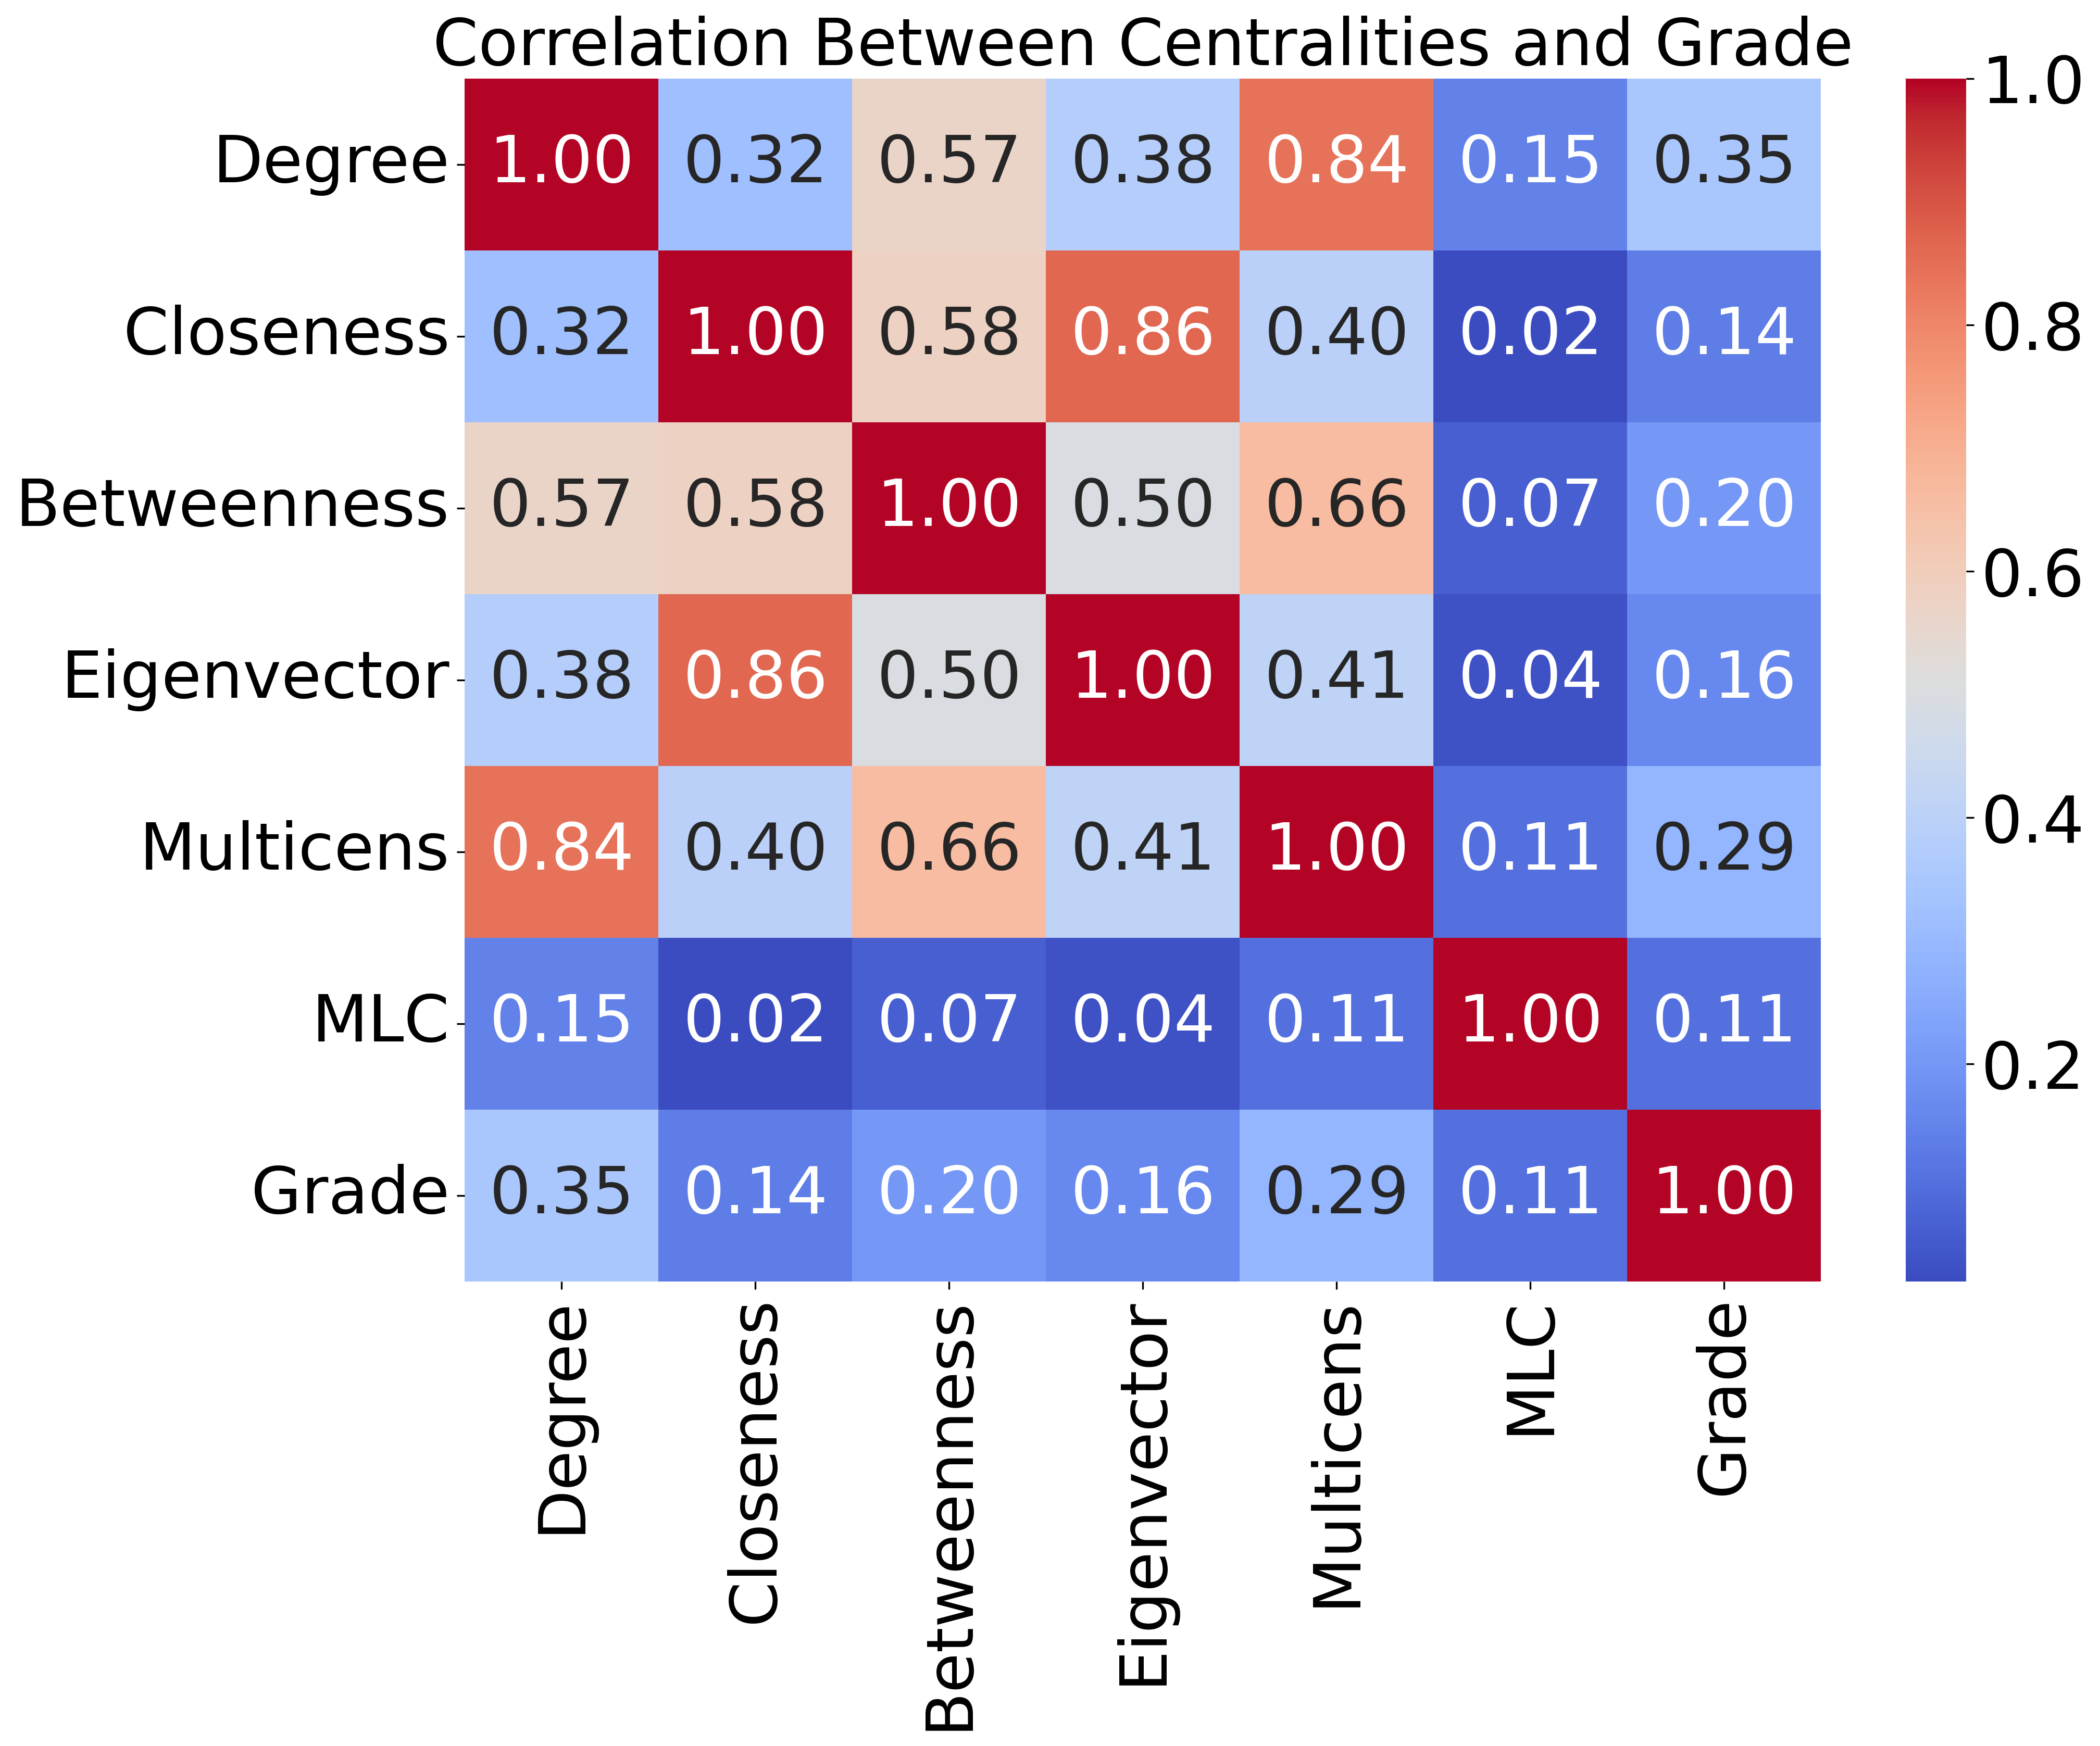
\includegraphics[width=\textwidth]{figs/fig31-hif2a_arnt-corr.png}
	\subcaption{}
\end{minipage}
\hspace{0.5cm}
\begin{minipage}[b]{0.28\linewidth}
	\centering
	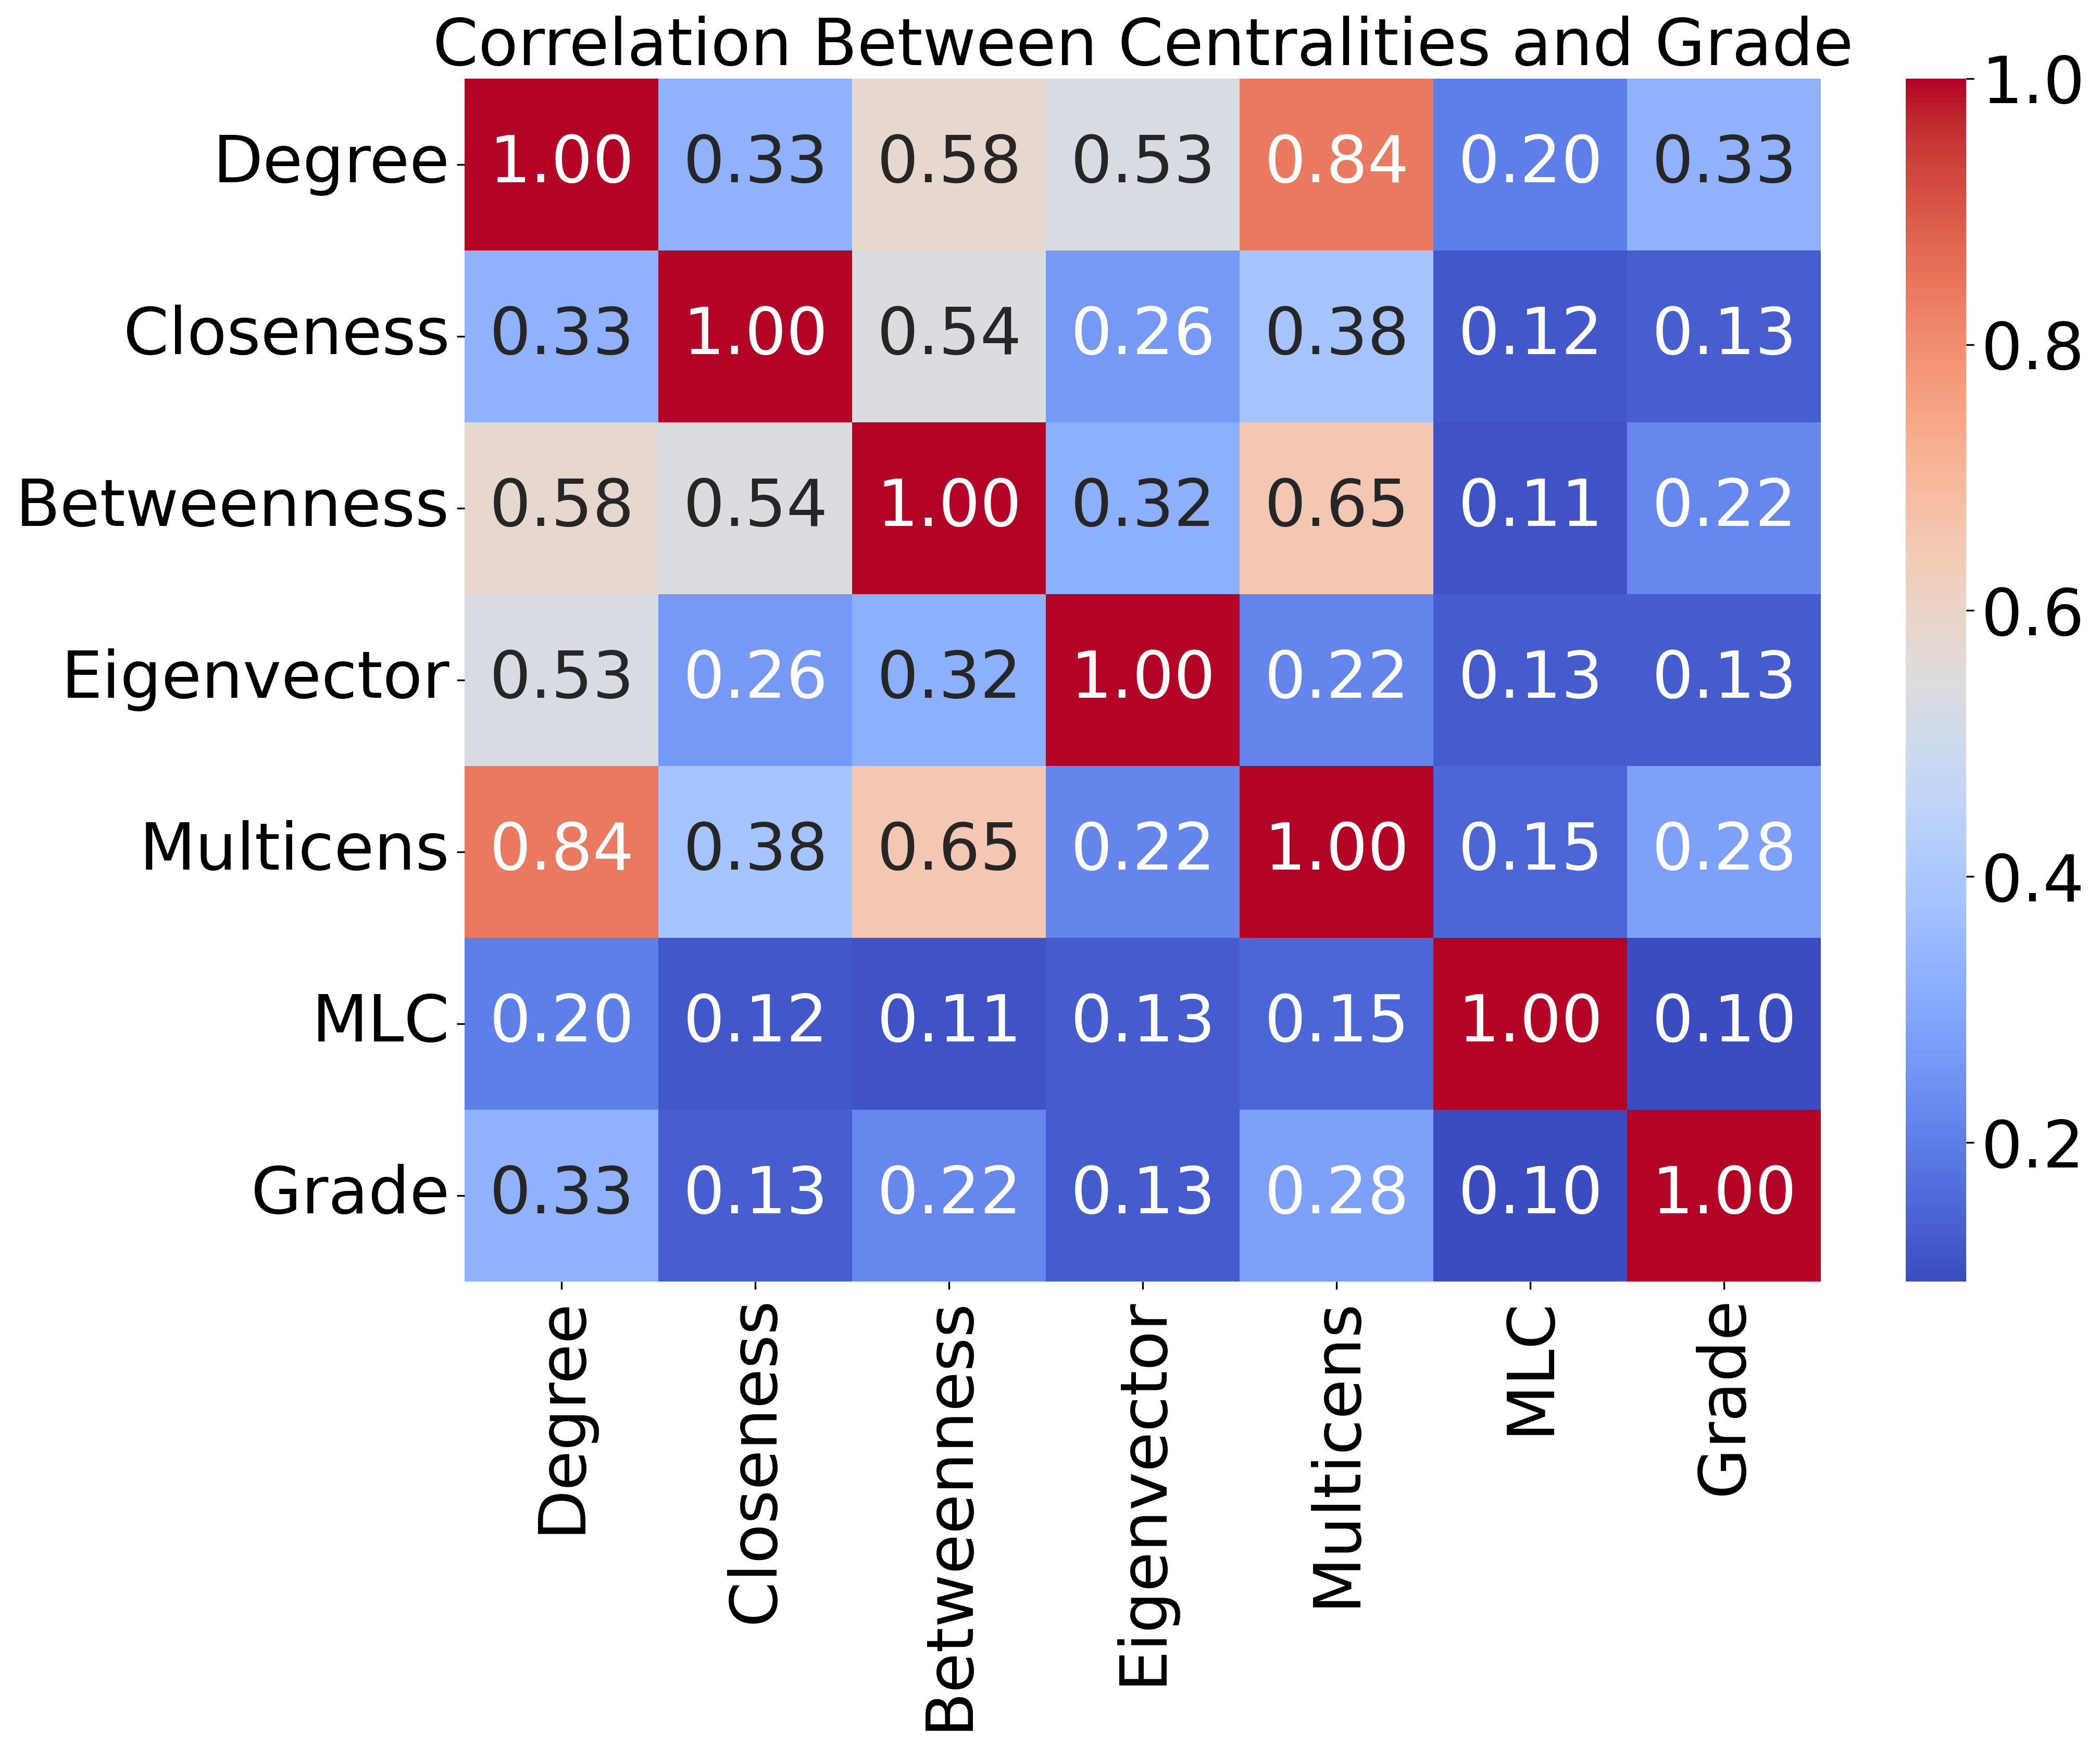
\includegraphics[width=\textwidth]{figs/fig32-hif3a_arnt-corr.png}
	\subcaption{}
\end{minipage}
\hspace{0.5cm}
\begin{minipage}[b]{0.28\linewidth}
	\centering
	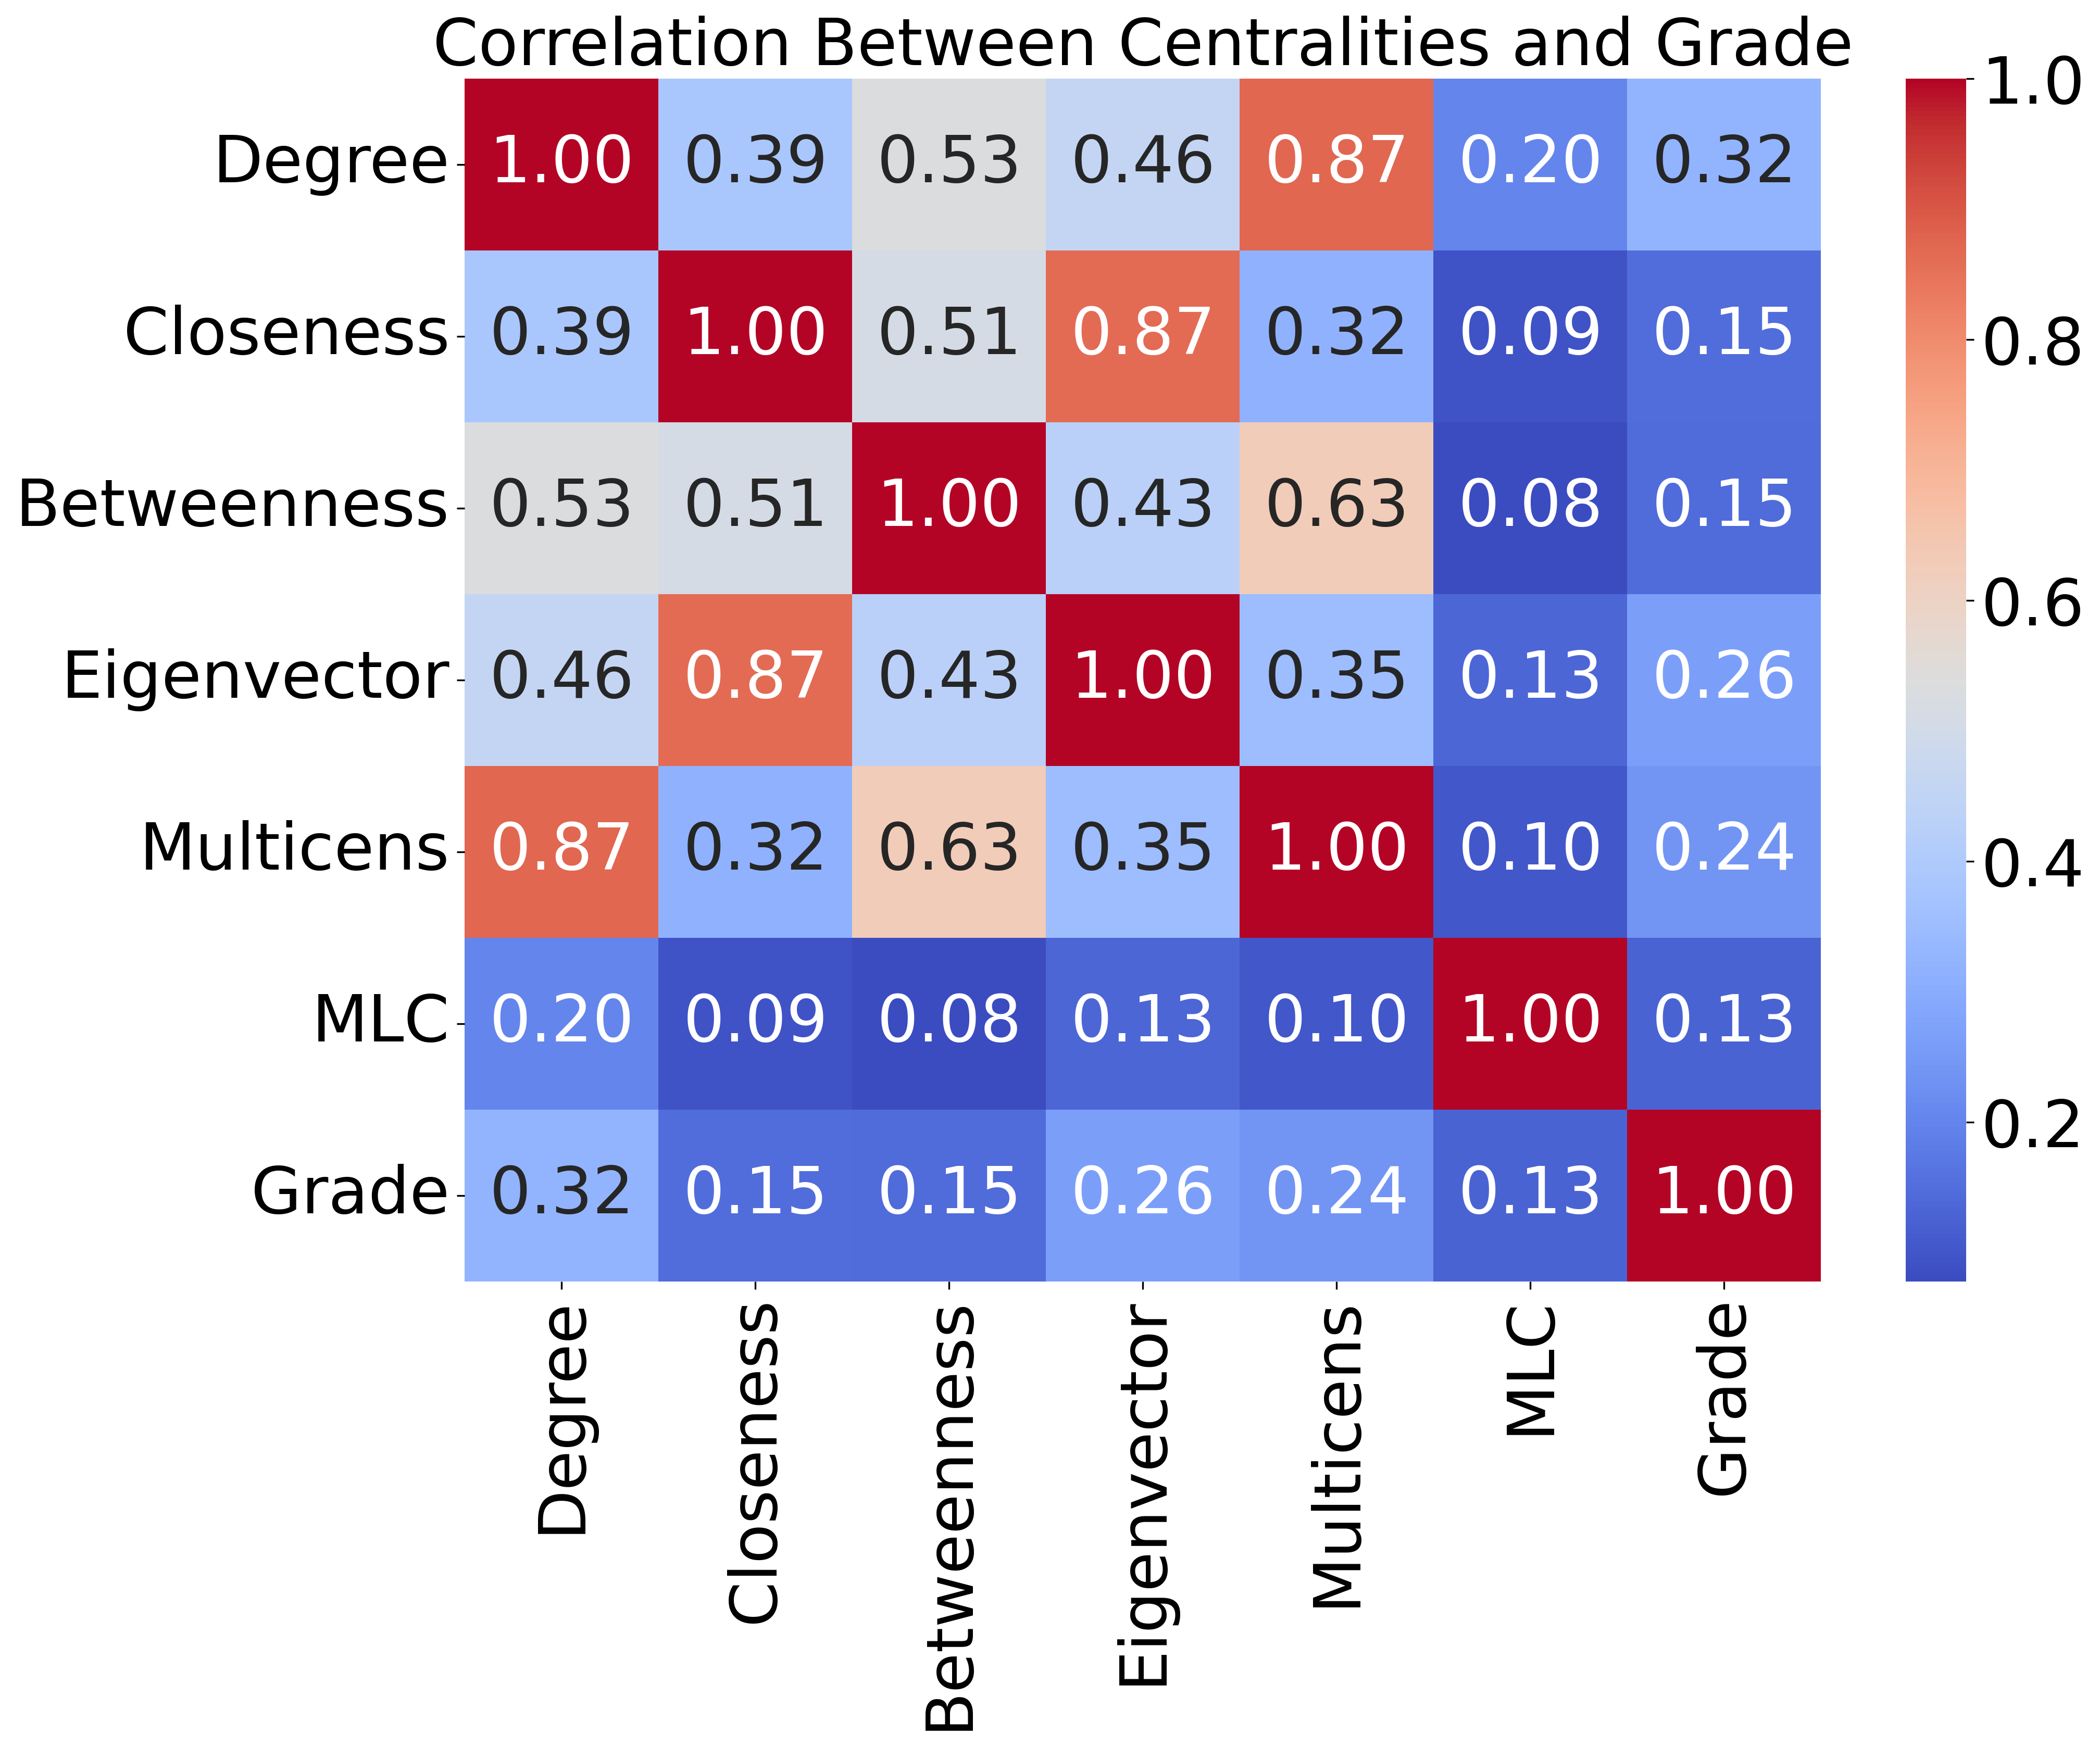
\includegraphics[width=\textwidth]{figs/fig33-npas1_arnt-corr.png}
	\subcaption{}
\end{minipage}

\vspace{0.5cm}

\begin{minipage}[b]{0.28\linewidth}
	\centering
	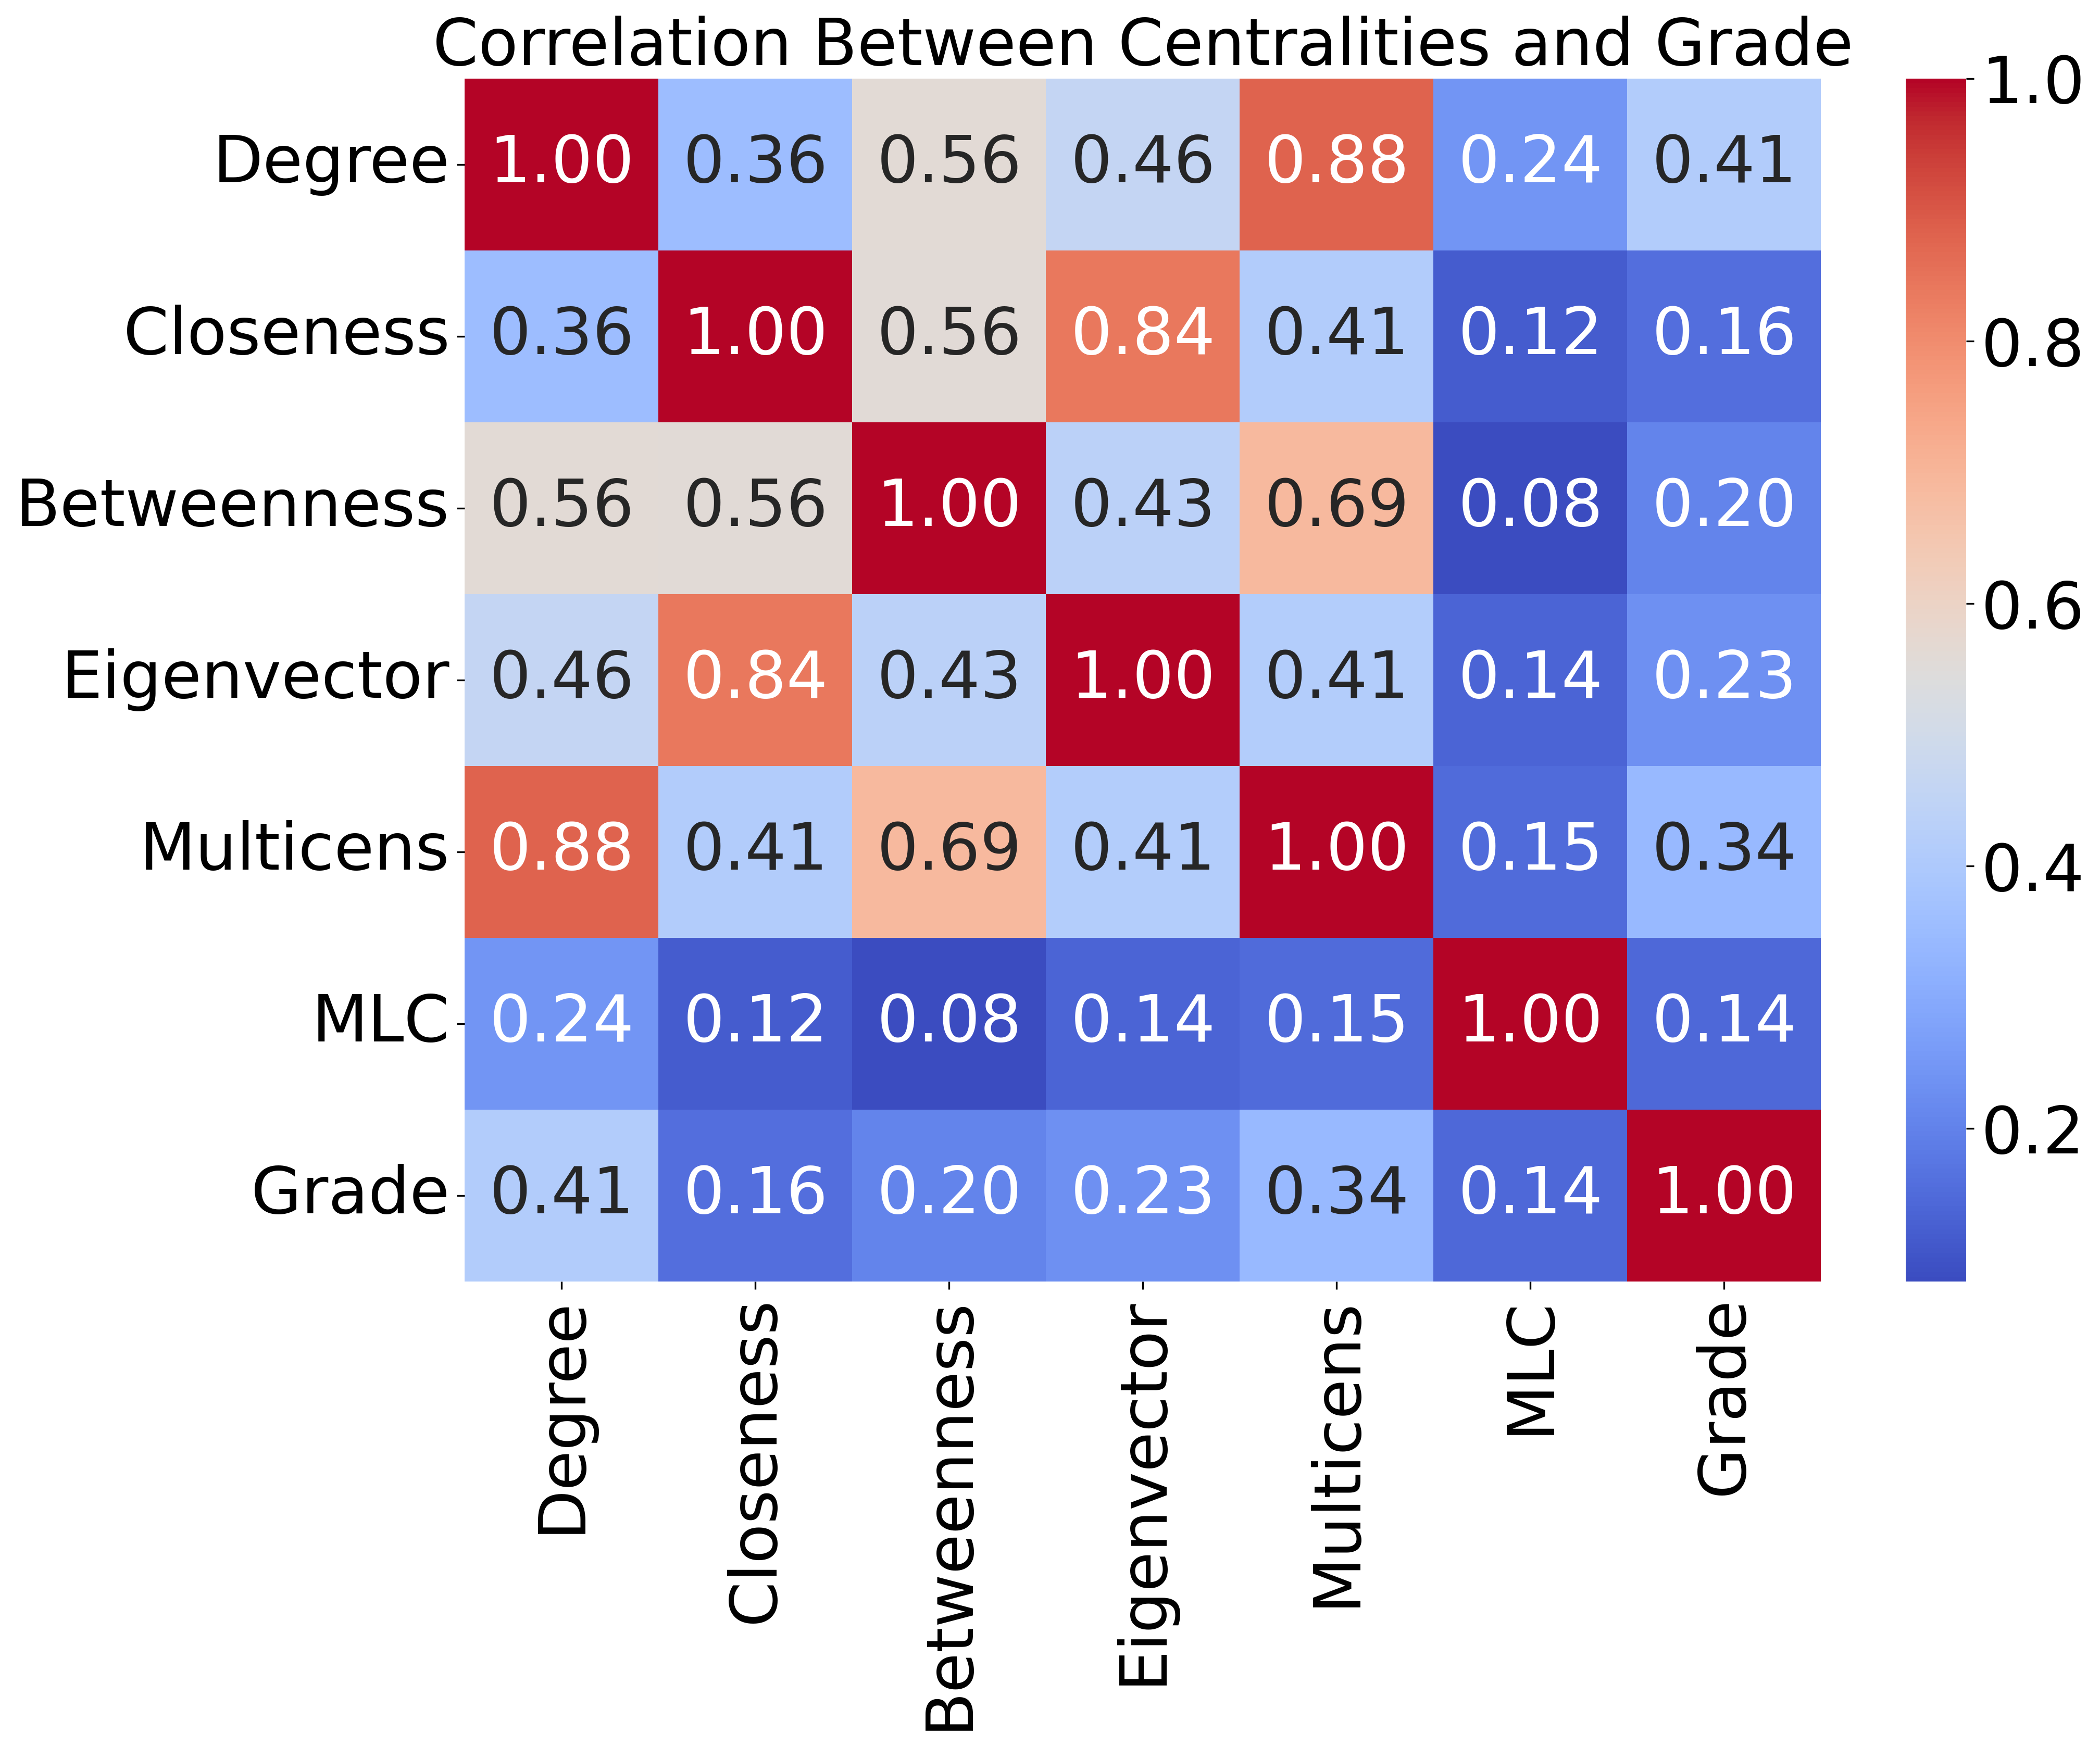
\includegraphics[width=\textwidth]{figs/fig34-npas2_bmal1-corr.png}
	\subcaption{}
\end{minipage}
\hspace{0.5cm}
\begin{minipage}[b]{0.28\linewidth}
	\centering
	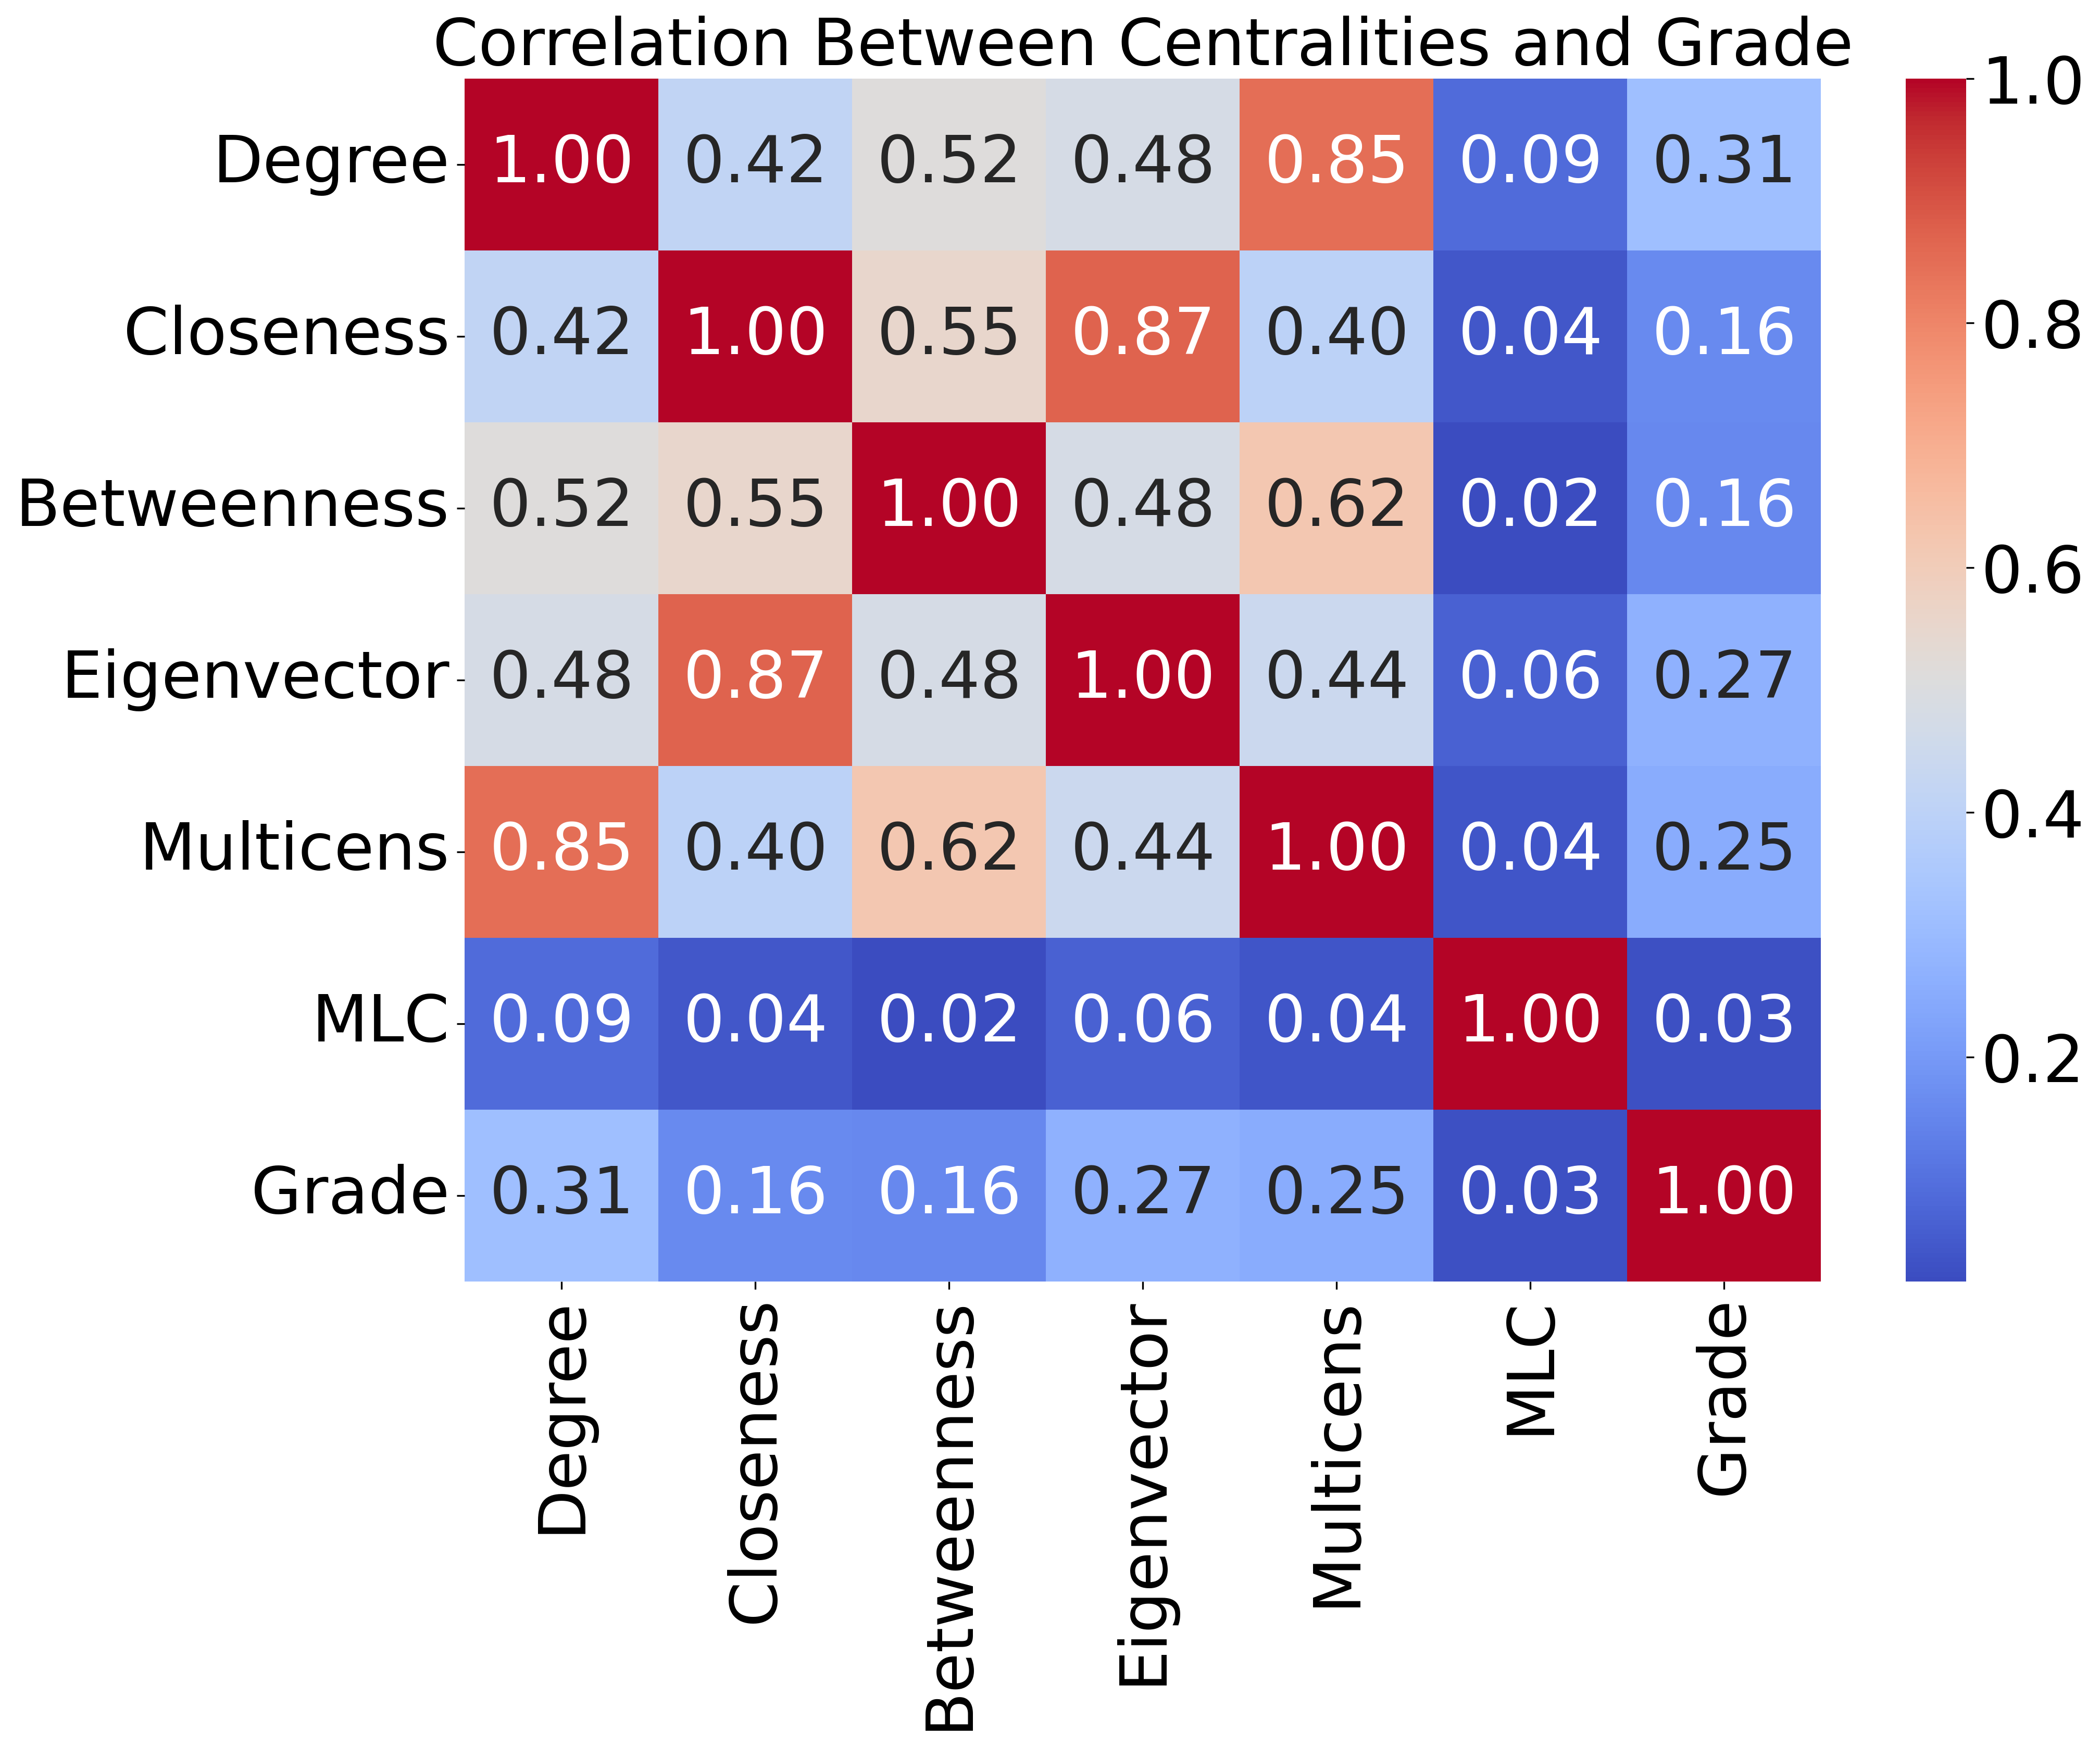
\includegraphics[width=\textwidth]{figs/fig35-npas3_arnt-corr.png}
	\subcaption{}
\end{minipage}
\hspace{0.5cm}
\begin{minipage}[b]{0.28\linewidth}
	\centering
	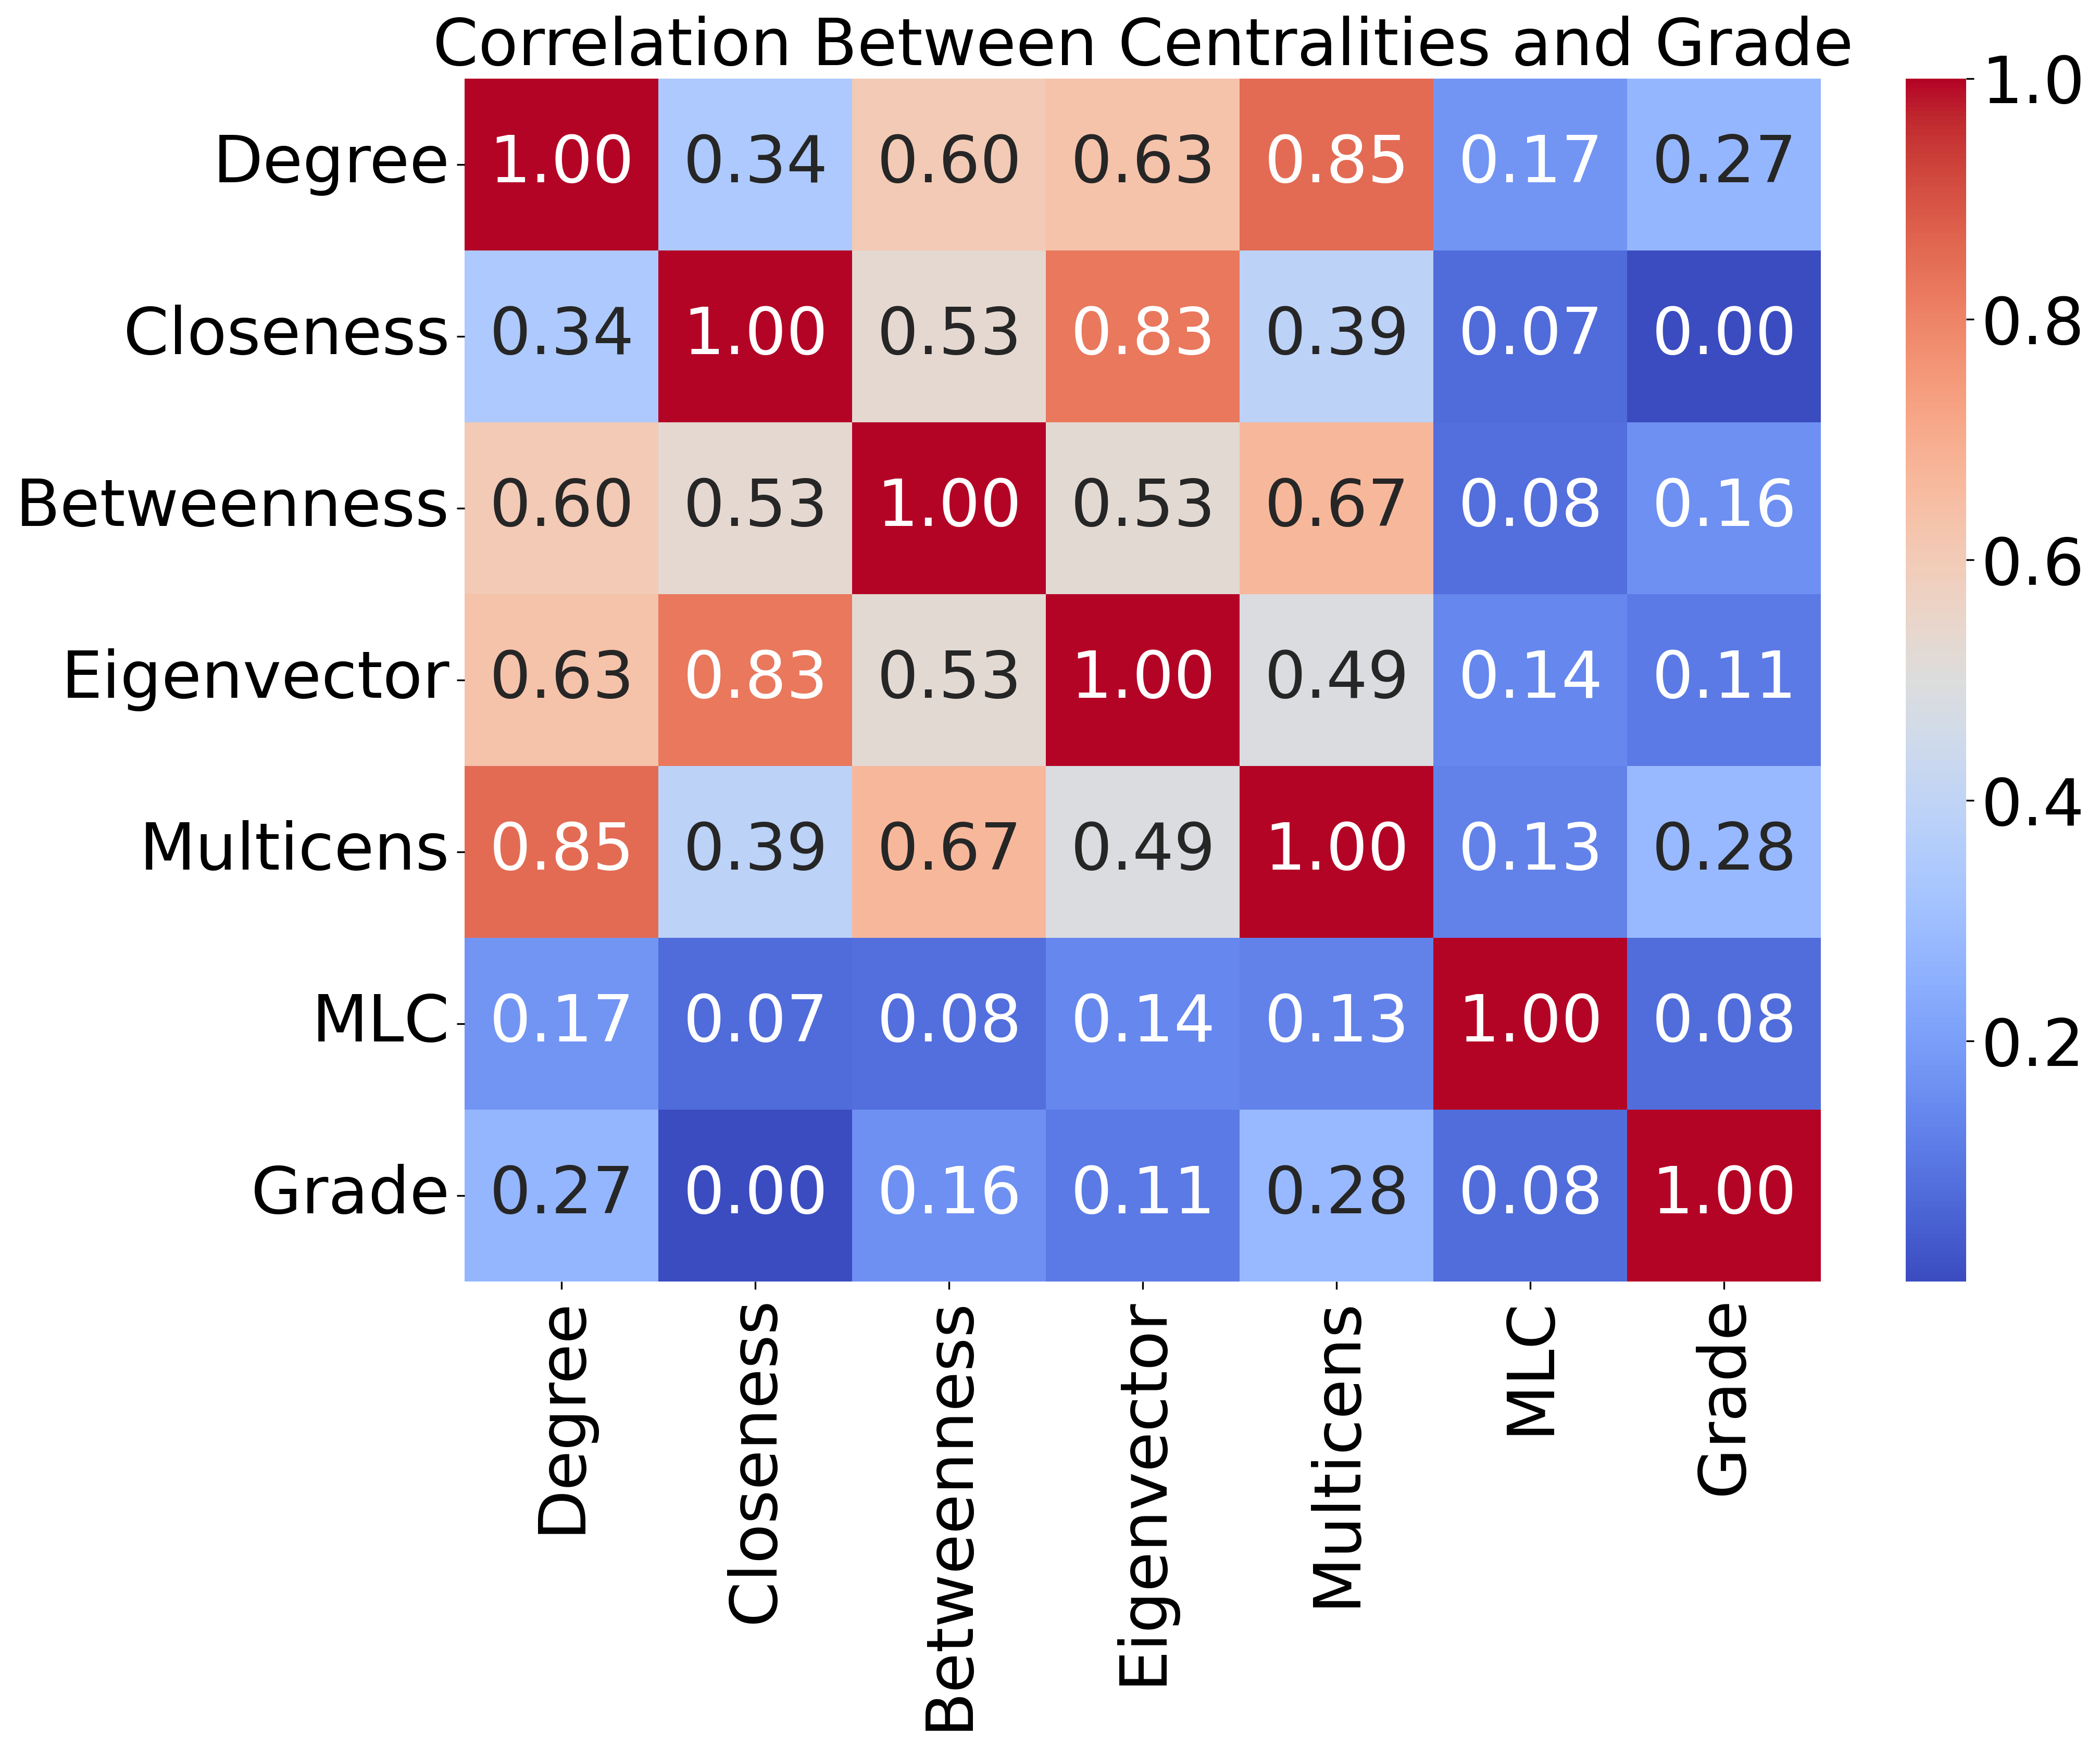
\includegraphics[width=\textwidth]{figs/fig36-npas4_arnt-corr.png}
	\subcaption{}
\end{minipage}

\vspace{0.5cm}

\begin{minipage}[b]{0.28\linewidth}
	\centering
	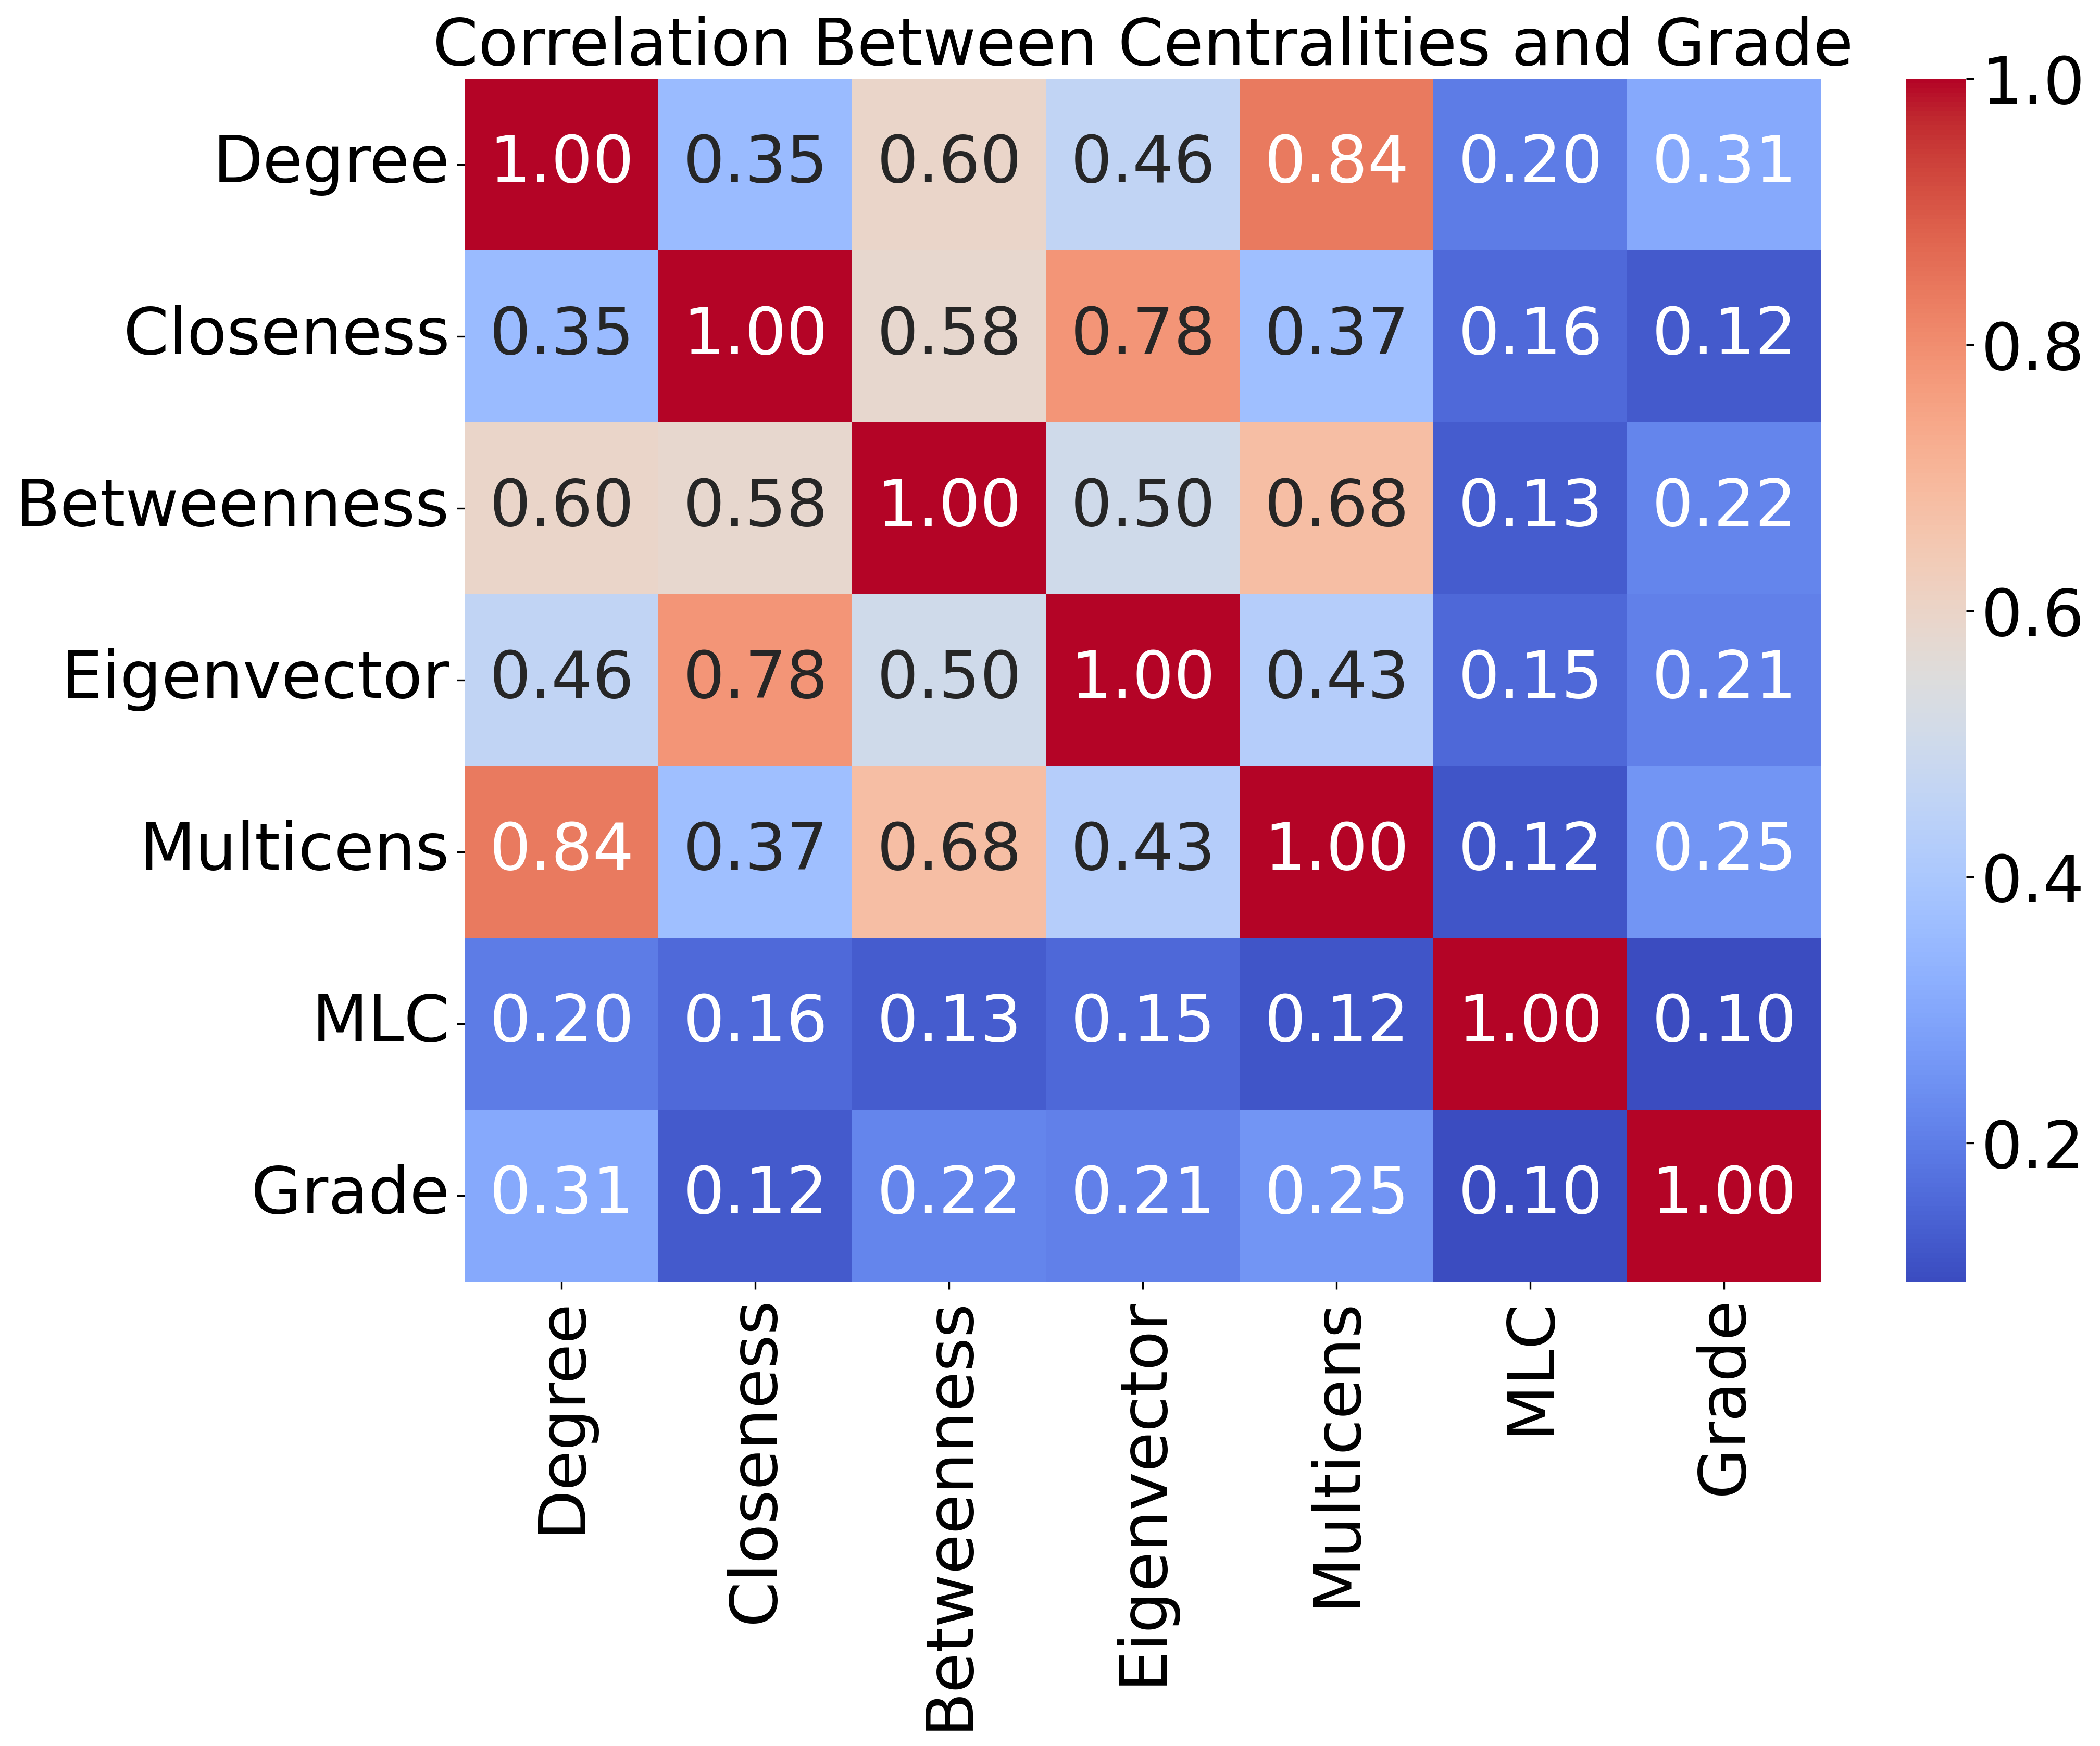
\includegraphics[width=\textwidth]{figs/fig37-sim1_arnt-corr.png}
	\subcaption{}
\end{minipage}
\hspace{0.5cm}
\begin{minipage}[b]{0.28\linewidth}
	\centering
	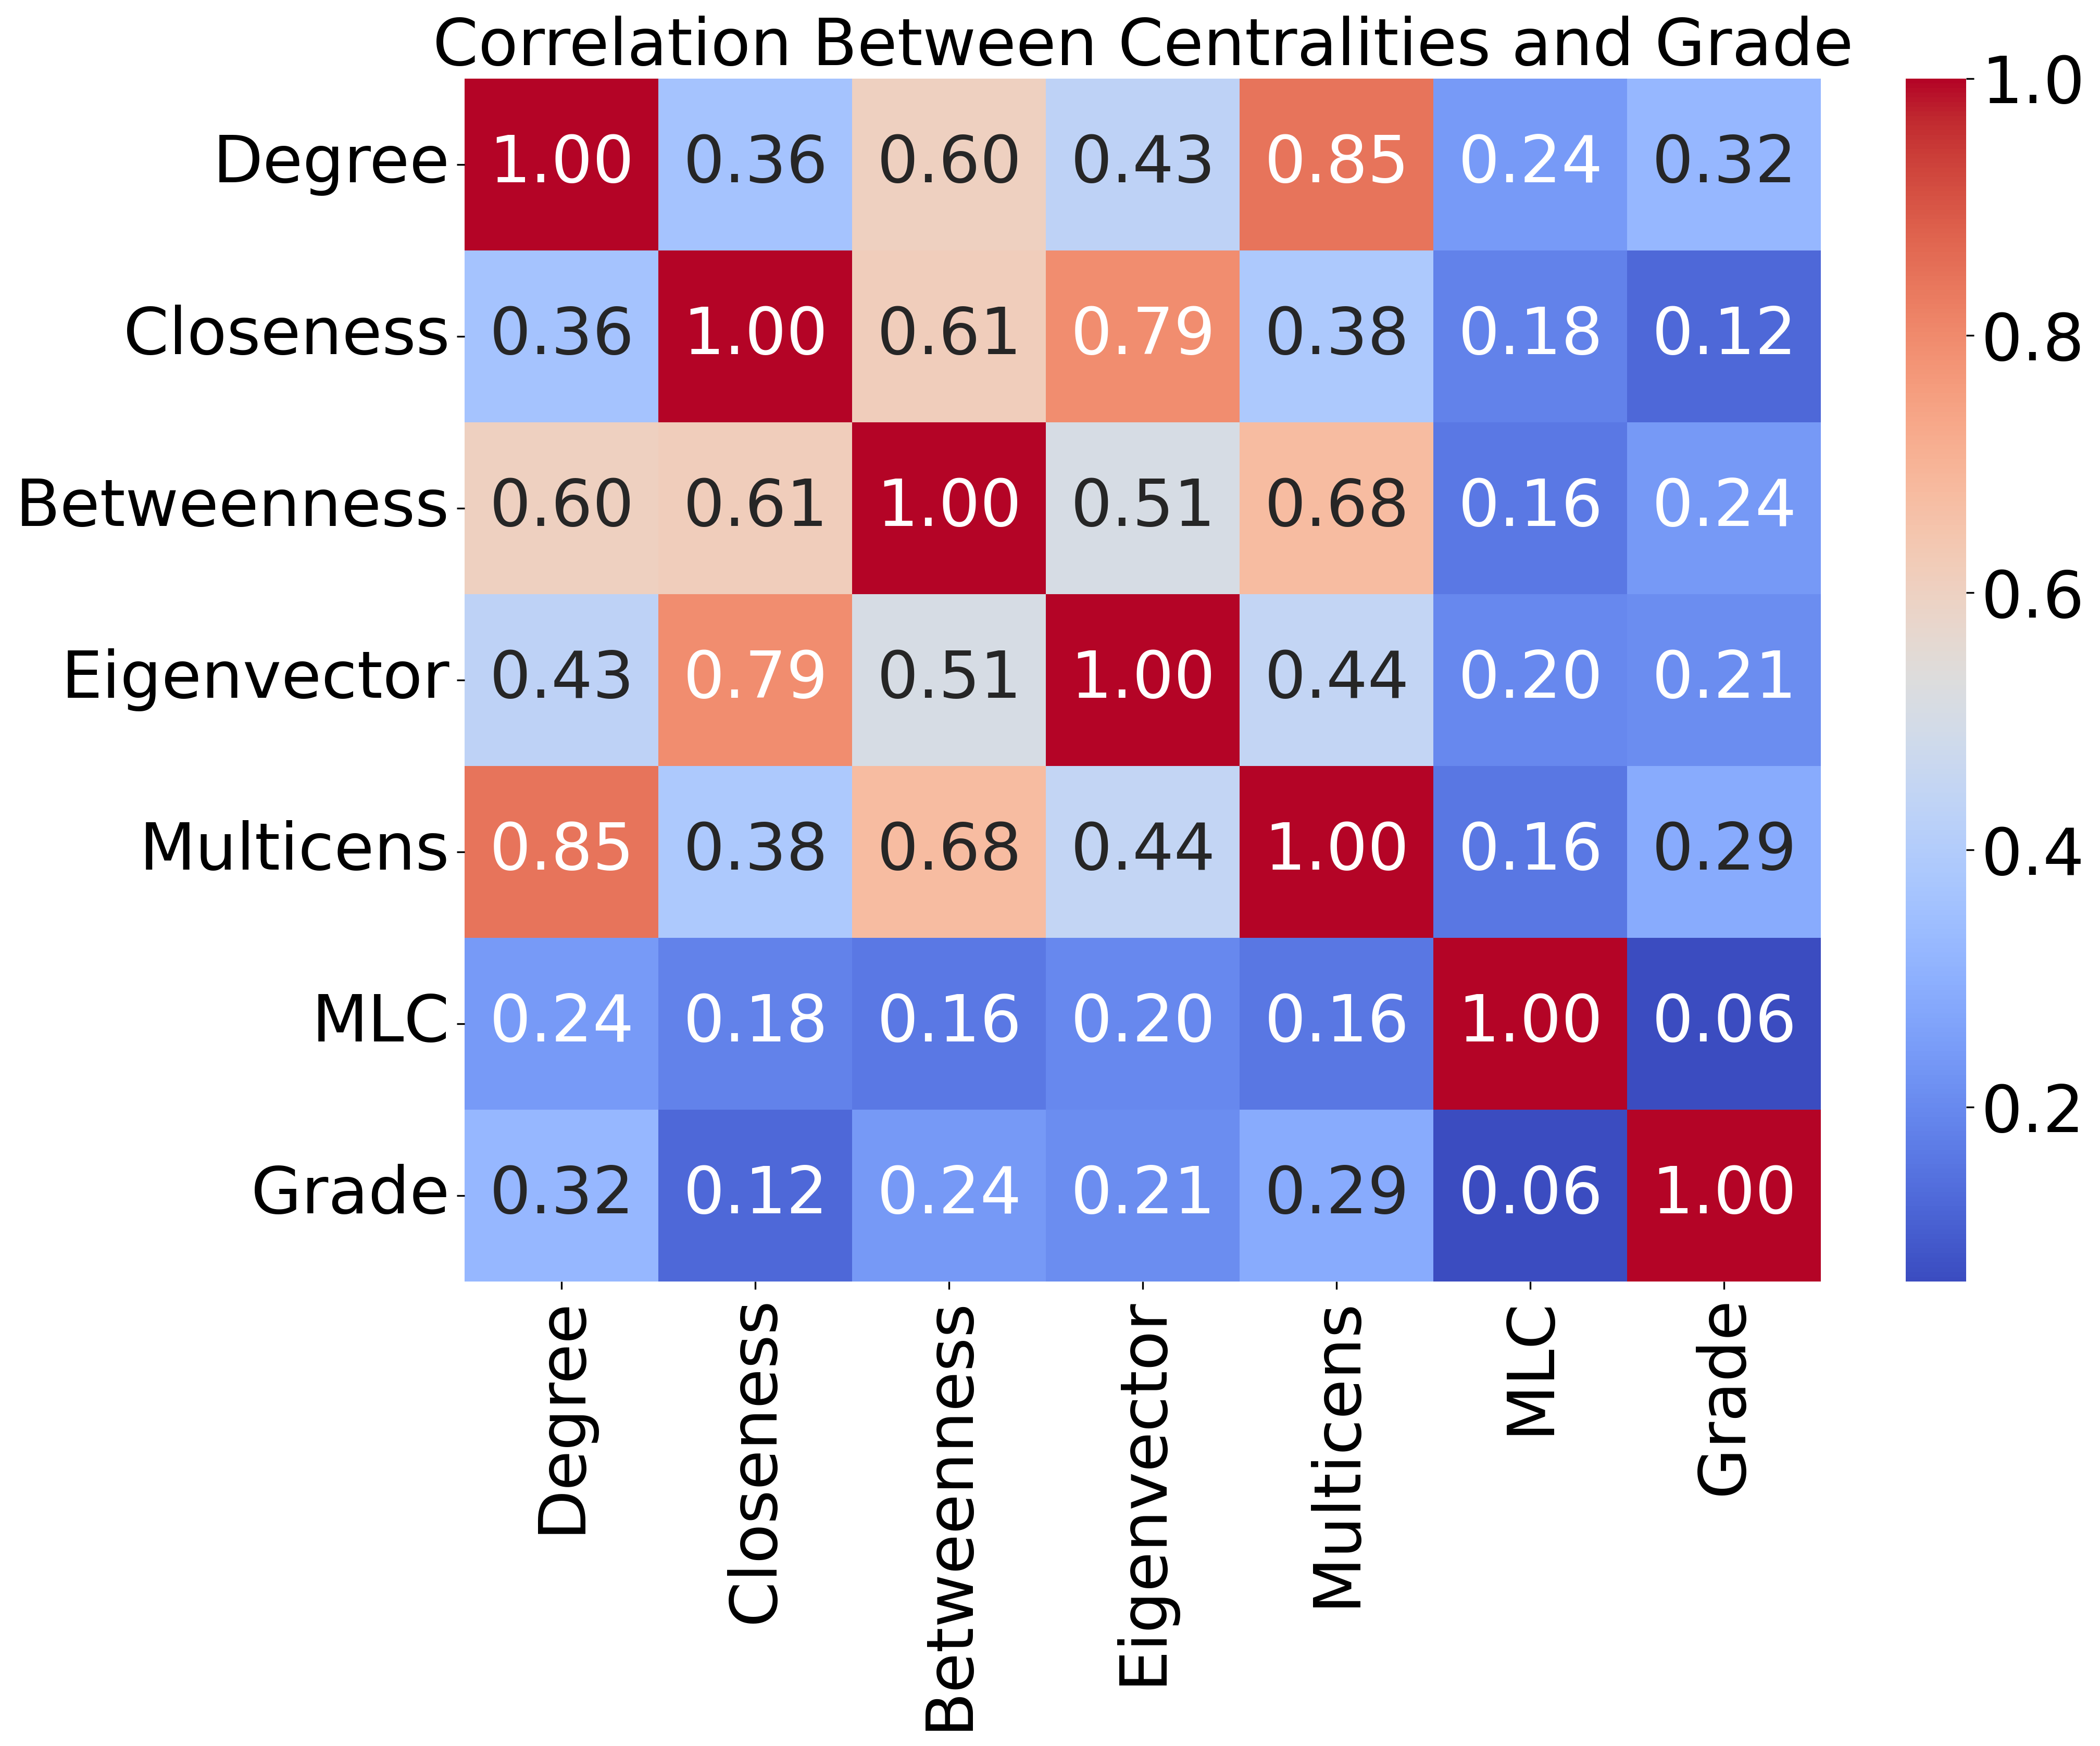
\includegraphics[width=\textwidth]{figs/fig38-sim2_arnt-corr.png}
	\subcaption{}
\end{minipage}

\caption{Correlation between degree, closeness, betweenness, eigenvector, multicens, and MLC centralities and conserved grade scores for proteins: (a) AHR-ARNT; (b) CLOCK-BMAL1; (c) HIF1A-ARNT; (d) HIF2A-ARNT; (e) HIF3A-ARNT; (f) NPAS1-ARNT; (g) NPAS2-BMAL1; (h) NPAS3-ARNT; (i) NPAS4-ARNT; (j) SIM1-ARNT; (k) SIM2-ARNT\label{fig:corr1}}
\end{figure}




\section*{Conclusion}




\section*{Acknowledgments}
Cras egestas velit mauris, eu mollis turpis pellentesque sit amet. Interdum et malesuada fames ac ante ipsum primis in faucibus. Nam id pretium nisi. Sed ac quam id nisi malesuada congue. Sed interdum aliquet augue, at pellentesque quam rhoncus vitae.

\nolinenumbers

\bibliographystyle{plain}
\bibliography{reference}

% Either type in your references using
% \begin{thebibliography}{}
% \bibitem{}
% Text
% \end{thebibliography}
%
% or
%
% Compile your BiBTeX database using our plos2015.bst
% style file and paste the contents of your .bbl file
% here. See http://journals.plos.org/plosone/s/latex for 
% step-by-step instructions.
% 
% \begin{thebibliography}{10}

% \bibitem{bib1}
% Conant GC, Wolfe KH.
% \newblock {{T}urning a hobby into a job: how duplicated genes find new
%   functions}.
% \newblock Nat Rev Genet. 2008 Dec;9(12):938--950.

% \bibitem{bib2}
% Ohno S.
% \newblock Evolution by gene duplication.
% \newblock London: George Alien \& Unwin Ltd. Berlin, Heidelberg and New York:
%   Springer-Verlag.; 1970.

% \bibitem{bib3}
% Magwire MM, Bayer F, Webster CL, Cao C, Jiggins FM.
% \newblock {{S}uccessive increases in the resistance of {D}rosophila to viral
%   infection through a transposon insertion followed by a {D}uplication}.
% \newblock PLoS Genet. 2011 Oct;7(10):e1002337.

% \end{thebibliography}



\end{document}

